\documentclass[11pt,letterpaper]{article}
\usepackage[utf8]{inputenc}
\usepackage[T1]{fontenc}
\usepackage[spanish,es-noshorthands,es-tabla]{babel}
\usepackage{lmodern}
\usepackage[margin=2.2cm]{geometry}
\usepackage{amsmath,amssymb}
\usepackage{graphicx}
\usepackage{booktabs,longtable}
\usepackage{float}
\usepackage{adjustbox}
\usepackage{pdflscape}
\usepackage[font=small,labelfont=bf]{caption}
\usepackage[hidelinks]{hyperref}
\setlength{\parskip}{0.45em}
\setlength{\parindent}{0pt}

\title{\textbf{Minority game de tres decisiones}\\[0.3em]
\large Reporte de resultados de las fases 9, 11 y 12}
\author{Héctor Quijano Munguía\\[0.2em]
\small Ingeniería Física, UADY\\
\small Asesores: Ricardo Mansilla Corona (UNAM) y Saul J. Díaz Ceballos (UADY)}
\date{18 de noviembre de 2026}

\begin{document}
\maketitle

\begin{abstract}
Este reporte reúne tres etapas. La fase~9 registra cuántos agentes eligen cada opción en cada turno, construye tres precios con esos conteos y calcula sobre ellos lo que pide el apartado~6.7 del protocolo: rendimientos, colas anchas, agrupamiento de la volatilidad, fracción de abstención y medidas informacionales de los precios codificados en símbolos. Con puntaje y $m=3$, 4 y 5 aparecen colas anchas y agrupamiento de la volatilidad; sin puntaje y con $m=6$, no. La fase~11 buscó la fase gaseosa del juego con $m=2$, $s=2$, aumentando $N$ hasta un millón de agentes, y no la encontró: los picos de $M(d)$ en $d=27$, 54 y 81 siguen en todos los valores de $N$. La fase~12 ajustó la función de Hill a $\log_{10}M(d)$ para cinco combinaciones de $m$ y $s$. La función describe la caída de $M(d)$ en los dos casos donde $M(d)$ decae ($m=1,s=1$ y $m=2,s=2$ desde $d=3$), y no describe nada en los otros tres, donde $M(d)$ es plana u oscila.
\end{abstract}

\tableofcontents
\newpage

\section{Modelo y método común}

\subsection{Reglas del juego}
Hay $N$ agentes y $K=3$ opciones: 0 (comprar), 1 (vender) y 2 (abstenerse). Cada agente tiene $s$ estrategias que leen los últimos $m$ resultados y prescriben una opción. ``Con puntaje'' significa que cada estrategia suma un punto virtual cuando habría elegido la opción ganadora y el agente juega con la de mayor puntaje; ``sin puntaje'' significa que el agente no califica sus estrategias. Las semillas son las 100 que se derivan de la semilla maestra 1907443528, iguales en todas las fases.

En estas fases se usaron dos reglas para decidir el ganador:
\begin{itemize}
\item \textbf{Regla vieja} (la de \texttt{reglas\_del\_modelo.md} y de las fases 2 a 8): gana la opción menos elegida, contando también una opción con cero agentes.
\item \textbf{Regla nueva}: una opción sin agentes no cuenta. Gana la menos elegida entre las que tienen al menos un agente, y si todos eligen la misma opción, gana esa y ganan todos.
\end{itemize}
En las dos, un empate entre las menos elegidas se decide con una moneda. Las fases 9 y 11 usan la regla nueva y la fase 12 la vieja, para poder compararla con las fases 7 y 8. \textbf{En ninguna corrida de estas tres fases hubo un solo turno con una opción vacía}, así que con estos parámetros las dos reglas dan exactamente el mismo juego.

\subsection{Medidas}
Información mutua en bits, $M(d)=\sum_{a,b}P_{ab}(d)\log_2[P_{ab}(d)/(P_aP_b)]$, con $d=1,\dots,100$, donde $P_a$ es la frecuencia de cada símbolo en toda la cadena. Complejidad física $C(l)=l\log_2 K-H(l)$, con $H(l)$ la entropía de las subcadenas de longitud $l$. Las medidas se calculan por cadena y se promedian sobre las 100 cadenas; los intervalos son del 95\,\%. $\gamma=K^m/N$ va en las tablas, no en los títulos de las gráficas.

\subsection{Corridas}
\begin{table}[H]
\centering\small
\caption{Corridas de este reporte. Todas con 100 cadenas y la semilla maestra 1907443528.}
\begin{tabular}{lllllll}
\toprule
Fase & Regla & $N$ & $m$ & $s$ & Puntaje & $T$\\
\midrule
9, precios & nueva & 101 & 2, 3 & 2 & con y sin & 6000\\
9, apartado 6.7 & nueva & 10000 & 2 a 6 & 2 & con y sin & 6000 (burn-in 1000)\\
11 & nueva & 101 a 1\,000\,000 (9 valores) & 2 & 2 & con & 6000\\
12 & vieja & 101 & 1, 2 & 0, 1, 2 & con & 60000\\
\bottomrule
\end{tabular}
\end{table}

\section{Fase 9: precios y series de tiempo}

\subsection{Precios con $N=101$}
Se agregó al juego el registro de $N_0$, $N_1$ y $N_2$ (cuántos agentes eligen cada opción) en cada turno, sin consumir números aleatorios, y con esos conteos se calcularon tres precios:
\begin{align*}
\text{Mansilla:}&\quad p_t=\arctan(N_0/N_1),\\
\text{Exceso de demanda:}&\quad \ln p_{t+1}=\ln p_t+(N_0-N_1)/\lambda_E,\qquad \lambda_E=N,\\
\text{Cociente:}&\quad \ln p_{t+1}=\ln p_t+\ln[(N_0+1)/(N_1+1)]/\lambda_C,\qquad \lambda_C=\ln(N+1),
\end{align*}
con $\ln p_0=0$ en los dos acumulados.

\textbf{Decisiones tomadas:} en Mansilla, si nadie vende $p=\pi/2$, si nadie compra $p=0$, y si nadie compra ni vende se repite el precio anterior ($\pi/4$ en el primer turno); ninguno de estos casos ocurrió. Las gráficas se hicieron sin burn-in (turnos 0 a 5999) y con burn-in de 1000 turnos (los acumulados vuelven a empezar en $\ln p=0$ en el turno 1000). La ``cadena destacada'' de cada caso es la de mayor recorrido (máximo menos mínimo) de $\ln p$ con exceso de demanda después del burn-in; se usa en todas las gráficas del caso.

\begin{table}[H]
\centering
\scriptsize
\setlength{\tabcolsep}{3.5pt}
\caption{Fase 9, $N=101$, $s=2$, $T=6000$, 100 cadenas (600\,000 turnos por caso). ``Vacías'' suma los turnos con una opción vacía, con $N_0=N_1=0$ y con todos en la misma opción. El recorrido es el de $\ln p$ con exceso de demanda después del burn-in. Las dos últimas columnas dan el rango, entre las 100 cadenas, del valor final de $\ln p$ (sin burn-in).}\label{tab:f9n101}
\begin{adjustbox}{max width=\textwidth}
\begin{tabular}{rrlrrlrrrrr}
\toprule
Caso & $m$ & Puntaje & $\gamma$ & Vacías & Moneda & Semilla destacada & Recorrido dest. & Recorrido mediano & $\ln p$ final, exceso & $\ln p$ final, cociente \\
\midrule
A & 2 & sin & 0.0891 & 0 & 40435 (6.7\,\%) & 2658800735 & 675.2 & 68.0 & $-$390.2 a 816.0 & $-$253.4 a 545.0 \\
B & 2 & con & 0.0891 & 0 & 35344 (5.9\,\%) & 4143265232 & 42.3 & 12.8 & $-$42.9 a 46.5 & $-$29.8 a 28.7 \\
C & 3 & sin & 0.2673 & 0 & 41404 (6.9\,\%) & 3939606599 & 215.4 & 40.7 & $-$258.3 a 133.3 & $-$162.2 a 85.1 \\
D & 3 & con & 0.2673 & 0 & 84085 (14.0\,\%) & 826721091 & 64.5 & 9.6 & $-$79.9 a 46.7 & $-$50.1 a 29.2 \\
\bottomrule
\end{tabular}
\end{adjustbox}
\end{table}


\subsubsection*{Observaciones}
\begin{itemize}
\item \textbf{Nunca hubo una opción vacía}, ni turnos con $N_0=N_1=0$ o con todos en la misma opción, así que la regla nueva no llegó a aplicarse y el precio de Mansilla nunca se repitió.
\item \textbf{Los precios acumulados se van casi en línea recta.} Cada cadena tiene un sesgo casi fijo entre compradores y vendedores, y al sumarlo 6000 veces el precio sube o baja sin parar. Sin puntaje el efecto es mayor (la cadena destacada del caso A llega a $\ln p\approx 816$); con puntaje es mucho menor, pero sigue ahí.
\item \textbf{El precio de Mansilla es una banda de ruido alrededor de $\pi/4$}, porque depende solo de los conteos del turno y no acumula nada. En el acercamiento de 200 turnos sí se distinguen sus variaciones.
\item \textbf{No se ven burbujas.} El precio de Mansilla no puede formar una subida sostenida, y en los acumulados se ve una tendencia fija, no una subida acelerada seguida de una caída. Esto es a ojo; no se aplicó ninguna prueba.
\end{itemize}
Las 16 gráficas están en el apéndice~\ref{ap:f9n101}.

\subsection{Complejidad de los precios codificados en binario ($N=101$)}
Como en Mansilla (Physica A 301, 2001), cada precio se convirtió en una serie binaria: 1 si subió respecto al turno anterior y 0 si bajó; los turnos sin cambio se omiten. Los precios de exceso de demanda y de cociente suben en los mismos turnos (cuando $N_0>N_1$), así que dan la misma serie (``acumulado''); el código lo verifica en las 400 cadenas. A cada serie se le calculó $C(l)$ con $l=1,\dots,8$ y se ajustó $C(l)=\beta\,l^{\alpha}$ en log-log con $l\ge 2$.

\begin{table}[H]
\centering
\footnotesize
\setlength{\tabcolsep}{3.5pt}
\caption{Fase 9, $N=101$: $C(l)$ de los precios codificados en binario, promedio de 100 cadenas. ``Omitidos'' es el promedio de turnos sin cambio de precio por cadena. Ajuste $C(l)=\beta l^\alpha$ con $l=2,\dots,8$.}\label{tab:f9ck}
\begin{adjustbox}{max width=\textwidth}
\begin{tabular}{rrllrrrrrrrr}
\toprule
Caso & $m$ & Puntaje & Serie & Burn-in & Omitidos & Frac. subidas & $C(2)$ & $C(8)$ & $\alpha$ & $\beta$ & $R^2$ \\
\midrule
A & 2 & sin & Mansilla & 0 & 42.5 & 0.502 & 0.104 & 0.917 & 1.541 & $3.96\times10^{-2}$ & 0.9923 \\
A & 2 & sin & Acumulado & 0 & 288.6 & 0.487 & 0.132 & 0.879 & 1.358 & $5.34\times10^{-2}$ & 0.9985 \\
A & 2 & sin & Mansilla & 1000 & 35.6 & 0.501 & 0.104 & 0.921 & 1.546 & $3.93\times10^{-2}$ & 0.9925 \\
A & 2 & sin & Acumulado & 1000 & 240.0 & 0.488 & 0.132 & 0.886 & 1.362 & $5.33\times10^{-2}$ & 0.9987 \\
B & 2 & con & Mansilla & 0 & 28.9 & 0.500 & $7.48\times10^{-2}$ & 0.653 & 1.542 & $2.77\times10^{-2}$ & 0.9955 \\
B & 2 & con & Acumulado & 0 & 238.8 & 0.500 & $1.60\times10^{-3}$ & 0.134 & 3.372 & $1.32\times10^{-4}$ & 0.9846 \\
B & 2 & con & Mansilla & 1000 & 24.2 & 0.500 & $7.48\times10^{-2}$ & 0.659 & 1.547 & $2.75\times10^{-2}$ & 0.9957 \\
B & 2 & con & Acumulado & 1000 & 199.1 & 0.500 & $1.64\times10^{-3}$ & 0.141 & 3.376 & $1.35\times10^{-4}$ & 0.9853 \\
C & 3 & sin & Mansilla & 0 & 38.5 & 0.499 & $8.90\times10^{-2}$ & 0.827 & 1.584 & $3.25\times10^{-2}$ & 0.9936 \\
C & 3 & sin & Acumulado & 0 & 282.7 & 0.484 & $3.99\times10^{-2}$ & 0.494 & 1.831 & $1.14\times10^{-2}$ & 0.9986 \\
C & 3 & sin & Mansilla & 1000 & 32.3 & 0.499 & $8.87\times10^{-2}$ & 0.830 & 1.589 & $3.23\times10^{-2}$ & 0.9938 \\
C & 3 & sin & Acumulado & 1000 & 235.5 & 0.484 & $3.99\times10^{-2}$ & 0.500 & 1.840 & $1.13\times10^{-2}$ & 0.9988 \\
D & 3 & con & Mansilla & 0 & 163.4 & 0.498 & $8.18\times10^{-2}$ & 0.715 & 1.538 & $3.09\times10^{-2}$ & 0.9932 \\
D & 3 & con & Acumulado & 0 & 623.9 & 0.494 & $1.06\times10^{-2}$ & 0.135 & 1.832 & $2.88\times10^{-3}$ & 0.9992 \\
D & 3 & con & Mansilla & 1000 & 145.1 & 0.498 & $8.24\times10^{-2}$ & 0.727 & 1.543 & $3.10\times10^{-2}$ & 0.9935 \\
D & 3 & con & Acumulado & 1000 & 538.7 & 0.494 & $1.10\times10^{-2}$ & 0.145 & 1.853 & $2.92\times10^{-3}$ & 0.9987 \\
\bottomrule
\end{tabular}
\end{adjustbox}
\end{table}


\begin{figure}[H]
\centering
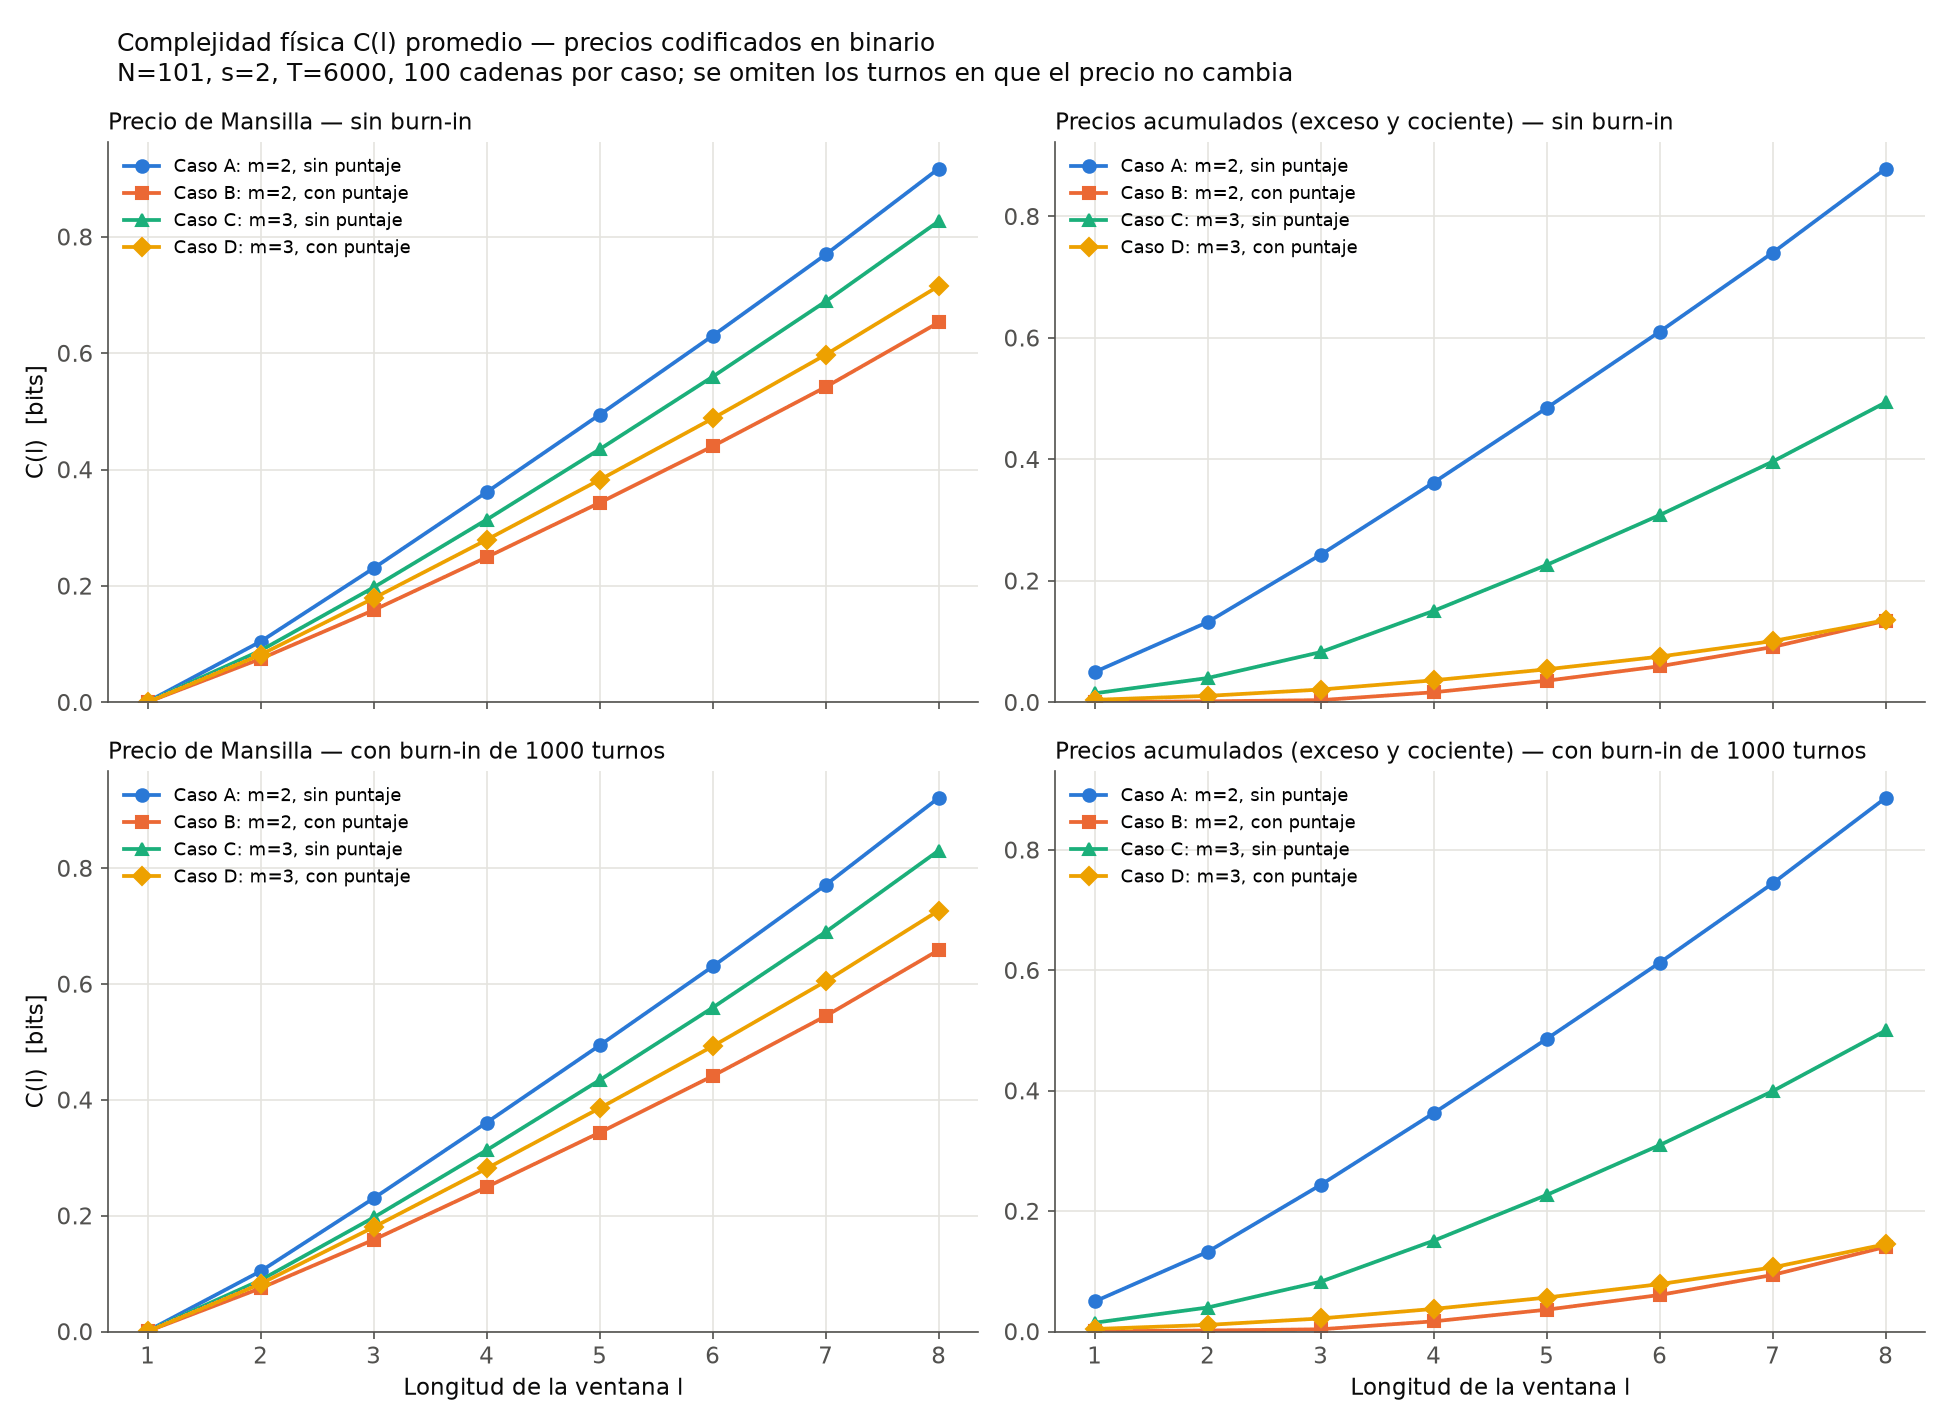
\includegraphics[width=0.85\textwidth]{figuras/Fase9_CK_contra_l_precios_binarios_N101_s2_T6000_regla_nueva.png}\\[0.5em]
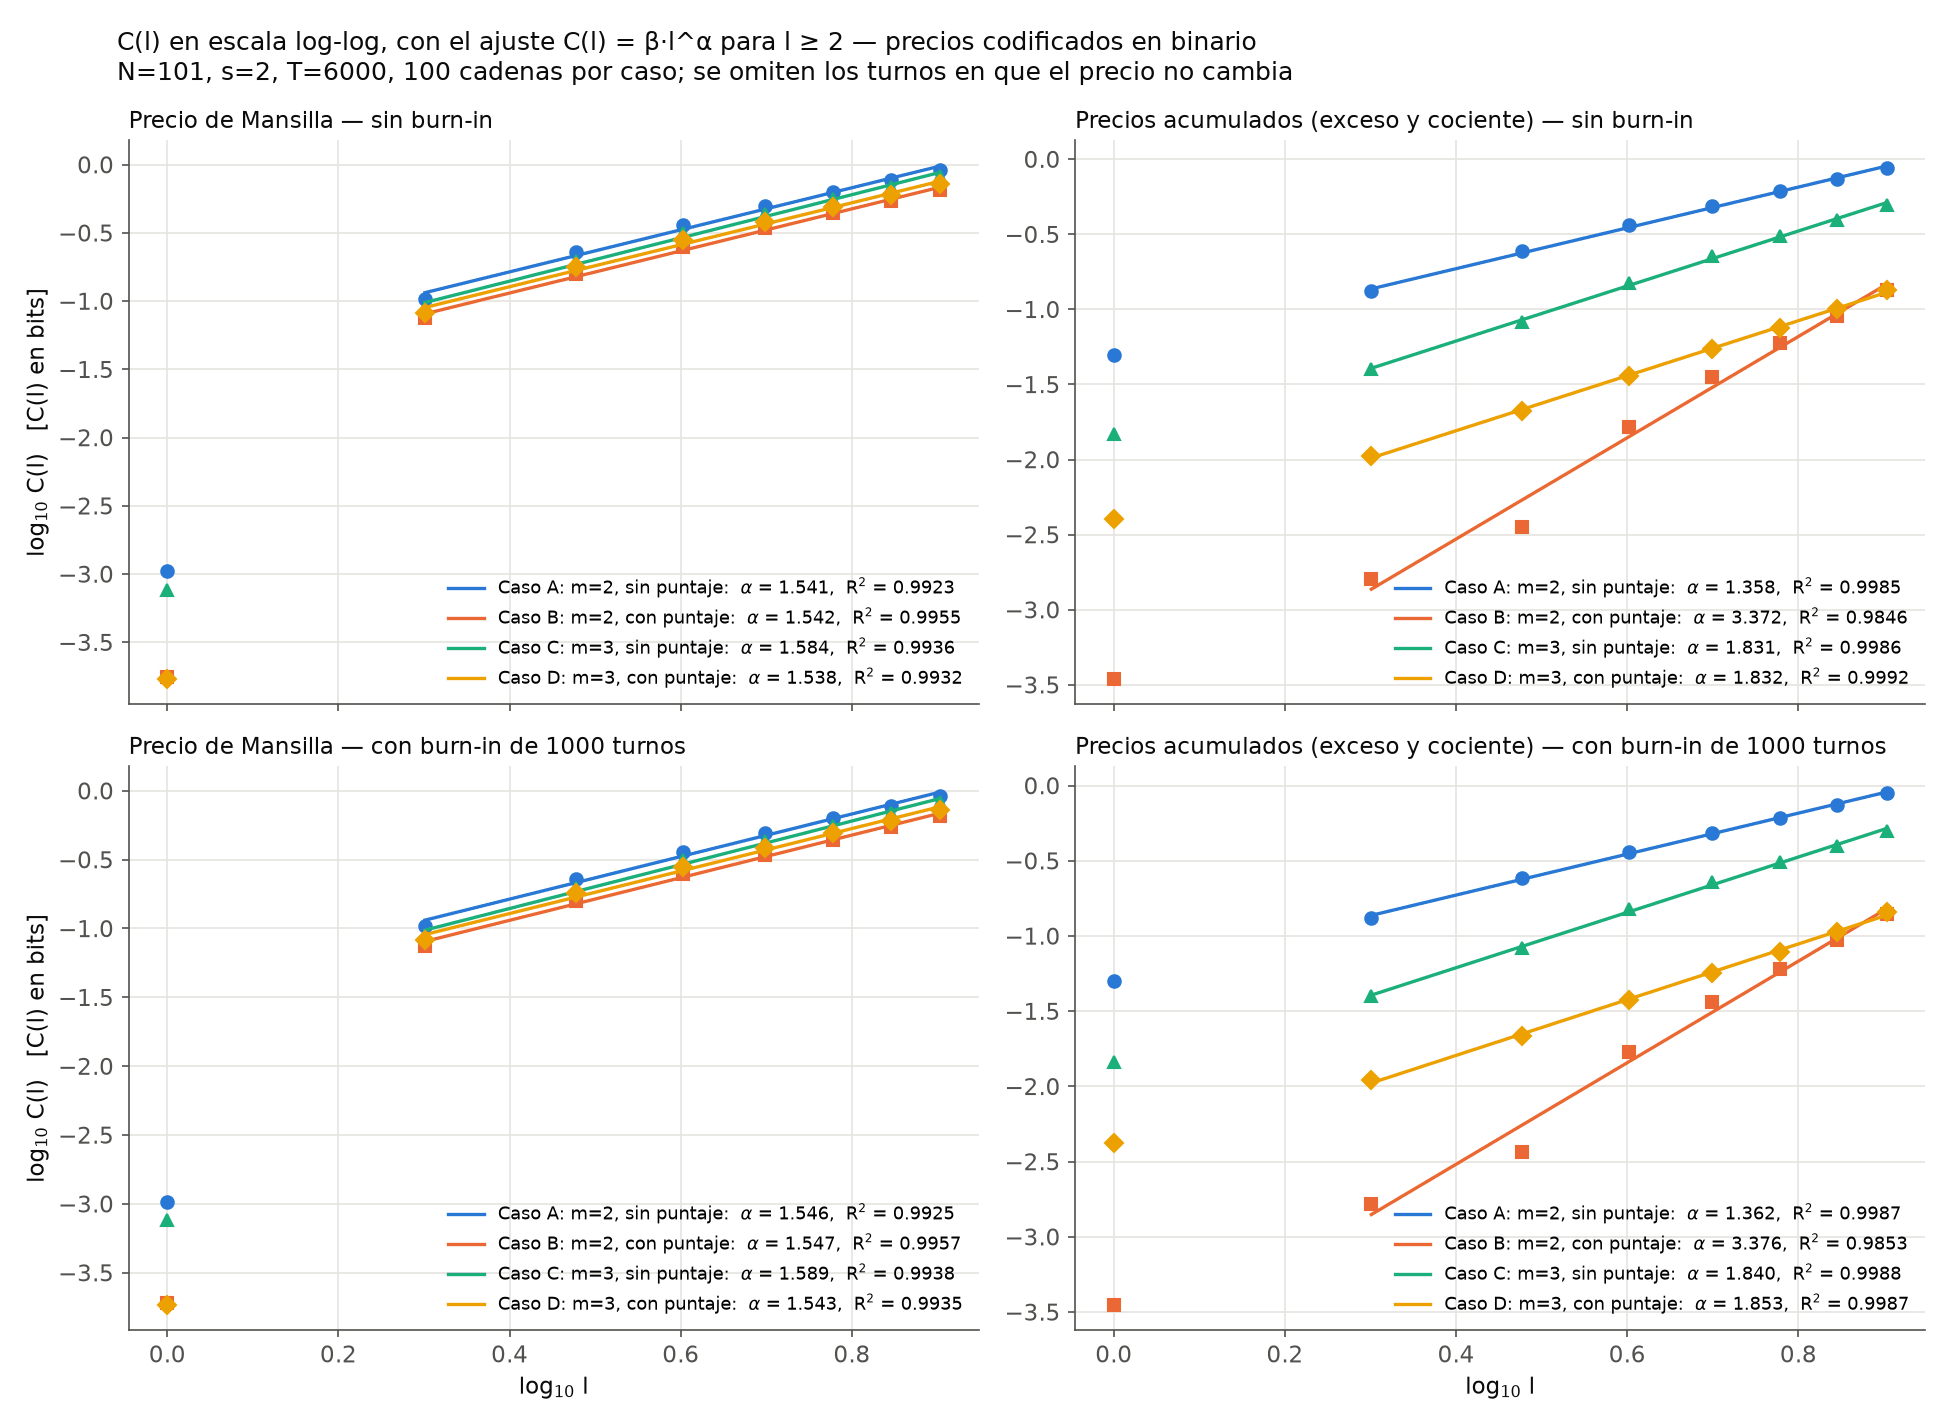
\includegraphics[width=0.85\textwidth]{figuras/Fase9_CK_loglog_precios_binarios_N101_s2_T6000_regla_nueva.png}
\caption{$C(l)$ de los precios codificados en binario, $N=101$. Arriba: $C(l)$ contra $l$. Abajo: log-log con el ajuste $C(l)=\beta l^\alpha$.}
\end{figure}

\subsubsection*{Observaciones}
\begin{itemize}
\item \textbf{Serie de Mansilla:} $\alpha\approx 1.54$ a 1.59 en los cuatro casos, casi sin diferencia entre ellos. Probablemente mide un efecto de la codificación y no del juego: como el precio de Mansilla no acumula, después de una subida es más probable una bajada, y eso solo da $C(2)\approx 0.082$ bits, cerca de lo obtenido (0.075 a 0.104). Ese valor lo calculé a mano y no lo comprobé con una corrida de referencia.
\item \textbf{Serie de los acumulados:} sí distingue los casos. Con puntaje $C(8)$ es mucho menor (0.13 a 0.15 contra 0.49 a 0.89 sin puntaje). El caso B tiene el exponente más alto, 3.37.
\item El artículo reporta $\alpha$ de 2.1 (periodo tranquilo) a 3.8 (antes de una caída) con series de 38\,000 a 168\,000 puntos. Aquí cada cadena tiene unos 5000 a 6000 símbolos y no se sabe qué valores de $l$ usó el artículo en su ajuste, así que la comparación es aproximada.
\end{itemize}

\subsection{Apartado 6.7 del protocolo con $N=10000$}
Siete casos con $N=10000$, $s=2$, $T=6000$ y burn-in de 1000 turnos: A ($m=2$, sin puntaje), B ($m=2$, con puntaje), C ($m=3$, sin puntaje), D ($m=3$, con puntaje), E ($m=4$), F ($m=5$) y G ($m=6$), estos tres con puntaje.

\textbf{Qué se calculó}, para cada uno de los tres precios:
\begin{itemize}
\item \textbf{Rendimientos} $r_t$: en los acumulados, el incremento de $\ln p$; en Mansilla, $r_t=\ln p_t-\ln p_{t-1}$. \textbf{Volatilidad} $|r_t|$. \textbf{Fracción que se abstiene} $f_2(t)=N_2/N$.
\item \textbf{Colas anchas:} curtosis (exceso sobre la normal, que vale 0) y exponente de la cola de $|r-\bar r|$ con el estimador de Hill sobre el 5\,\% de valores más grandes. Un exponente chico significa colas más anchas. Este estimador no tiene relación con la función de Hill de la fase 12.
\item \textbf{Agrupamiento de la volatilidad:} autocorrelación de $|r_t|$ para retardos 1 a 100 y su exponente de decaimiento (menos la pendiente log-log, solo con retardos de valor positivo).
\item \textbf{Codificación binaria:} 1 si el precio sube y 0 si baja, omitiendo los cambios nulos. \textbf{Ternaria:} 2 si $|r_t|<u\,\sigma_r$, con $u=0.1$, 0.25 y 0.5, y si no, 1 si sube y 0 si baja.
\item \textbf{Medidas informacionales} de cada serie simbólica: $C(l)$ con el ajuste $\beta l^\alpha$ ($l\ge 2$), $M(d)$ con su ajuste log-log, y el espectro de potencias de $M(d)$ (Ec.~4 del protocolo) con el ajuste $S\sim 1/f^{a}$.
\end{itemize}
Todo se calculó sin burn-in y con burn-in. Aquí se muestra la versión con burn-in; la versión sin burn-in está en el apéndice~\ref{ap:sinburnin}.

\begin{table}[H]
\centering
\scriptsize
\setlength{\tabcolsep}{3.5pt}
\caption{Fase 9, $N=10000$, $s=2$, $T=6000$, 100 cadenas: conteos y fracción de abstención $f_2=N_2/N$ (media y desviación estándar temporal, promediadas sobre las cadenas). ``Vacías'' como en la tabla~\ref{tab:f9n101}.}\label{tab:f9n10000}
\begin{adjustbox}{max width=\textwidth}
\begin{tabular}{rrlrrlrrrrr}
\toprule
Caso & $m$ & Puntaje & $\gamma$ & Vacías & Moneda & $f_2$ media & $f_2$ desv. & Semilla destacada & Recorrido dest. & Recorrido mediano \\
\midrule
A & 2 & sin & 0.00090 & 0 & 4435 (0.74\,\%) & 0.3335 & 0.0047 & 793465836 & 48.48 & 7.65 \\
B & 2 & con & 0.00090 & 0 & 2507 (0.42\,\%) & 0.3316 & 0.0616 & 2892114663 & 172.07 & 52.86 \\
C & 3 & sin & 0.00270 & 0 & 4333 (0.72\,\%) & 0.3336 & 0.0048 & 2855055785 & 64.31 & 4.42 \\
D & 3 & con & 0.00270 & 0 & 2516 (0.42\,\%) & 0.3329 & 0.0388 & 2512000159 & 64.92 & 18.71 \\
E & 4 & con & 0.00810 & 0 & 2589 (0.43\,\%) & 0.3334 & 0.0235 & 1254338790 & 20.85 & 6.28 \\
F & 5 & con & 0.02430 & 0 & 2672 (0.45\,\%) & 0.3334 & 0.0141 & 784491124 & 6.71 & 3.10 \\
G & 6 & con & 0.07290 & 0 & 3205 (0.53\,\%) & 0.3333 & 0.0065 & 3151201844 & 2.23 & 1.05 \\
\bottomrule
\end{tabular}
\end{adjustbox}
\end{table}


\begin{table}[H]
\centering
\footnotesize
\setlength{\tabcolsep}{3.5pt}
\caption{Fase 9, $N=10000$, con burn-in: hechos estilizados de los rendimientos. $\sigma_r$ es la desviación estándar de $r$; la curtosis es el exceso sobre la normal; el exponente de la cola usa el estimador de Hill con el 5\,\% más grande de $|r-\bar r|$; acf es la autocorrelación de $|r|$, y su exponente es menos la pendiente log-log, ajustada con los retardos de valor positivo (columna ``Puntos'').}\label{tab:f9hechos}
\begin{adjustbox}{max width=\textwidth}
\begin{tabular}{rrllrrrrrrrrr}
\toprule
Caso & $m$ & Punt. & Precio & $\sigma_r$ & Curtosis & Exp. cola & acf(1) & acf(10) & acf(100) & Exp. acf & $R^2$ acf & Puntos \\
\midrule
A & 2 & sin & Mansilla & $2.08\times10^{-2}$ & $-$0.084 & 6.31 & 0.196 & 0.002 & 0.0025 & 0.844 & 0.328 & 45 \\
A & 2 & sin & Exceso & $7.93\times10^{-3}$ & $-$0.140 & 6.43 & 0.005 & 0.008 & 0.0004 & 0.612 & 0.286 & 71 \\
A & 2 & sin & Cociente & $2.58\times10^{-3}$ & $-$0.138 & 6.43 & 0.005 & 0.008 & 0.0004 & 0.621 & 0.308 & 71 \\
B & 2 & con & Mansilla & 0.298 & 0.473 & 6.44 & 0.246 & $-$0.029 & $-$0.0204 & 0.052 & 0.002 & 29 \\
B & 2 & con & Exceso & 0.106 & $-$0.320 & 8.31 & 0.006 & $-$0.038 & $-$0.0229 & $-$0.381 & 0.130 & 36 \\
B & 2 & con & Cociente & $3.63\times10^{-2}$ & 0.164 & 6.13 & 0.022 & $-$0.040 & $-$0.0243 & $-$0.132 & 0.016 & 36 \\
C & 3 & sin & Mansilla & $2.15\times10^{-2}$ & $-$0.037 & 6.26 & 0.228 & 0.005 & $-$0.0009 & 0.886 & 0.458 & 40 \\
C & 3 & sin & Exceso & $8.06\times10^{-3}$ & $-$0.060 & 6.26 & 0.002 & 0.003 & $-$0.0002 & 0.744 & 0.345 & 49 \\
C & 3 & sin & Cociente & $2.62\times10^{-3}$ & $-$0.058 & 6.25 & 0.002 & 0.003 & $-$0.0002 & 0.766 & 0.357 & 49 \\
D & 3 & con & Mansilla & 0.185 & 1.542 & 4.74 & 0.282 & 0.005 & $-$0.0069 & 0.207 & 0.057 & 44 \\
D & 3 & con & Exceso & $6.71\times10^{-2}$ & 0.079 & 6.00 & 0.127 & 0.011 & $-$0.0057 & 0.036 & 0.002 & 49 \\
D & 3 & con & Cociente & $2.25\times10^{-2}$ & 0.730 & 5.18 & 0.147 & 0.013 & $-$0.0069 & 0.075 & 0.006 & 49 \\
E & 4 & con & Mansilla & 0.112 & 2.407 & 3.97 & 0.307 & 0.072 & $-$0.0393 & 1.163 & 0.665 & 44 \\
E & 4 & con & Exceso & $4.06\times10^{-2}$ & 0.645 & 5.22 & 0.201 & 0.089 & $-$0.0506 & 1.030 & 0.559 & 46 \\
E & 4 & con & Cociente & $1.35\times10^{-2}$ & 1.318 & 4.80 & 0.217 & 0.095 & $-$0.0529 & 1.054 & 0.555 & 46 \\
F & 5 & con & Mansilla & $6.74\times10^{-2}$ & 3.649 & 3.53 & 0.327 & 0.135 & 0.0188 & 0.605 & 0.826 & 100 \\
F & 5 & con & Exceso & $2.46\times10^{-2}$ & 1.406 & 4.46 & 0.267 & 0.165 & 0.0257 & 0.554 & 0.803 & 100 \\
F & 5 & con & Cociente & $8.13\times10^{-3}$ & 1.926 & 4.25 & 0.278 & 0.171 & 0.0258 & 0.564 & 0.804 & 100 \\
G & 6 & con & Mansilla & $3.05\times10^{-2}$ & $-$0.182 & 6.67 & 0.196 & 0.004 & 0.0036 & 0.261 & 0.261 & 100 \\
G & 6 & con & Exceso & $1.13\times10^{-2}$ & $-$0.470 & 7.39 & 0.020 & 0.006 & 0.0072 & 0.131 & 0.189 & 100 \\
G & 6 & con & Cociente & $3.68\times10^{-3}$ & $-$0.468 & 7.40 & 0.020 & 0.006 & 0.0073 & 0.130 & 0.193 & 100 \\
\bottomrule
\end{tabular}
\end{adjustbox}
\end{table}


\begin{table}[H]
\centering
\scriptsize
\setlength{\tabcolsep}{3.5pt}
\caption{Fase 9, $N=10000$, con burn-in: medidas informacionales de la serie binaria (1 = sube, 0 = baja). Exceso y cociente dan la misma serie binaria, así que aparecen juntos como ``Acumulados''. ``Frac. 1'' es la fracción de subidas. $C(l)=\beta l^\alpha$ con $l\ge2$; pendiente y $R^2$ del ajuste log-log de $M(d)$ con $d=1,\dots,100$; $a$ es el exponente del espectro de $M(d)$, $S\sim 1/f^a$.}\label{tab:f9bin}
\begin{adjustbox}{max width=\textwidth}
\begin{tabular}{rrllrrrrrrrrrrrr}
\toprule
Caso & $m$ & Punt. & Serie & Frac. 1 & $C(2)$ & $C(8)$ & $\alpha$ & $R^2_C$ & $M(1)$ & $M_{\max}$ & $d_{\max}$ & Pend. $M$ & $R^2_M$ & $a$ & $R^2_S$ \\
\midrule
A & 2 & sin & Mansilla & 0.502 & $9.07\times10^{-2}$ & 0.853 & 1.590 & 0.9924 & $8.81\times10^{-2}$ & $8.81\times10^{-2}$ & 1 & $-$0.760 & 0.567 & 0.321 & 0.930 \\
A & 2 & sin & Acumulados & 0.515 & 0.134 & 1.025 & 1.457 & 0.9974 & $3.51\times10^{-2}$ & $3.51\times10^{-2}$ & 1 & $-$1.046 & 0.878 & 1.346 & 0.809 \\
B & 2 & con & Mansilla & 0.502 & $7.72\times10^{-2}$ & 0.797 & 1.661 & 0.9985 & $7.54\times10^{-2}$ & $7.54\times10^{-2}$ & 1 & $-$0.547 & 0.358 & 0.111 & 0.208 \\
B & 2 & con & Acumulados & 0.501 & $4.25\times10^{-3}$ & 0.364 & 3.357 & 0.9888 & $1.87\times10^{-3}$ & $1.11\times10^{-2}$ & 3 & $-$0.390 & 0.270 & 0.179 & 0.021 \\
C & 3 & sin & Mansilla & 0.498 & $8.89\times10^{-2}$ & 0.794 & 1.556 & 0.9945 & $8.80\times10^{-2}$ & $8.80\times10^{-2}$ & 1 & $-$0.739 & 0.581 & 0.182 & 0.853 \\
C & 3 & sin & Acumulados & 0.494 & $5.55\times10^{-2}$ & 0.557 & 1.677 & 0.9996 & $1.45\times10^{-2}$ & $1.45\times10^{-2}$ & 1 & $-$0.946 & 0.822 & 1.264 & 0.839 \\
D & 3 & con & Mansilla & 0.499 & $7.76\times10^{-2}$ & 0.678 & 1.536 & 0.9944 & $7.72\times10^{-2}$ & $7.72\times10^{-2}$ & 1 & $-$0.475 & 0.385 & 0.021 & 0.273 \\
D & 3 & con & Acumulados & 0.501 & $8.60\times10^{-4}$ & $8.02\times10^{-2}$ & 3.410 & 0.9793 & $3.41\times10^{-4}$ & $2.36\times10^{-3}$ & 4 & $-$0.247 & 0.427 & 0.323 & 0.503 \\
E & 4 & con & Mansilla & 0.500 & $8.18\times10^{-2}$ & 0.685 & 1.506 & 0.9939 & $8.16\times10^{-2}$ & $8.16\times10^{-2}$ & 1 & $-$0.305 & 0.198 & 0.000 & 0.004 \\
E & 4 & con & Acumulados & 0.499 & $3.04\times10^{-4}$ & $4.28\times10^{-2}$ & 3.576 & 0.9711 & $1.26\times10^{-4}$ & $2.79\times10^{-4}$ & 5 & 0.010 & 0.003 & 0.199 & 0.033 \\
F & 5 & con & Mansilla & 0.500 & $8.16\times10^{-2}$ & 0.688 & 1.510 & 0.9938 & $8.15\times10^{-2}$ & $8.15\times10^{-2}$ & 1 & $-$0.271 & 0.161 & 0.000 & 0.009 \\
F & 5 & con & Acumulados & 0.499 & $2.52\times10^{-4}$ & $3.56\times10^{-2}$ & 3.529 & 0.9695 & $1.08\times10^{-4}$ & $2.52\times10^{-4}$ & 6 & 0.064 & 0.114 & 0.323 & 0.066 \\
G & 6 & con & Mansilla & 0.500 & $8.11\times10^{-2}$ & 0.682 & 1.508 & 0.9937 & $8.10\times10^{-2}$ & $8.10\times10^{-2}$ & 1 & $-$0.251 & 0.138 & $-$0.001 & 0.012 \\
G & 6 & con & Acumulados & 0.500 & $2.23\times10^{-4}$ & $3.29\times10^{-2}$ & 3.571 & 0.9748 & $8.09\times10^{-5}$ & $2.12\times10^{-4}$ & 81 & 0.091 & 0.239 & 0.359 & 0.048 \\
\bottomrule
\end{tabular}
\end{adjustbox}
\end{table}


\begin{figure}[H]
\centering
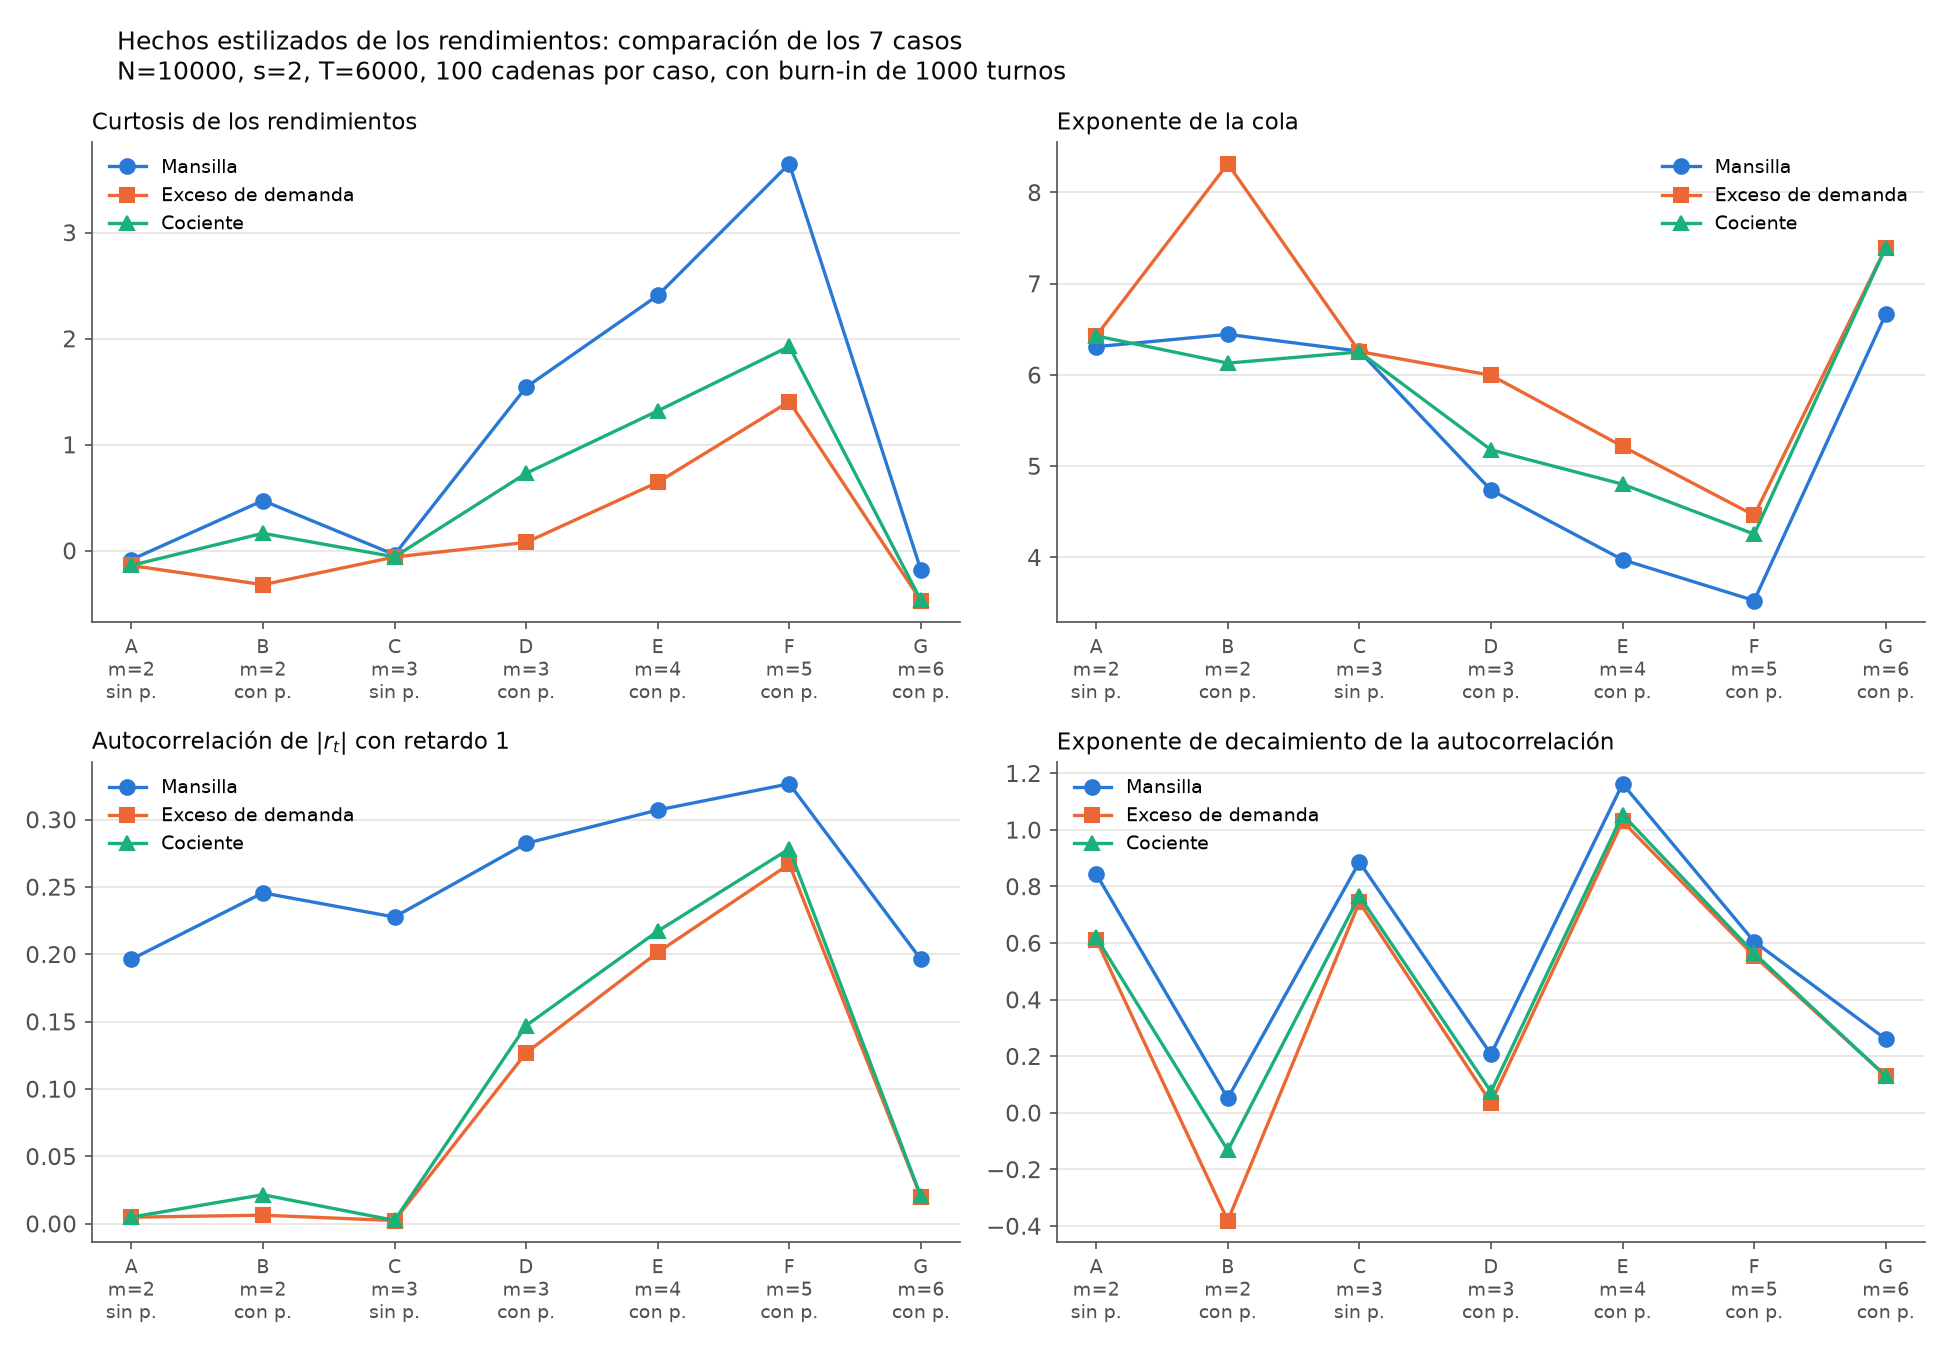
\includegraphics[width=0.95\textwidth]{figuras/Fase9_comparacion_hechos_estilizados_N10000_s2_T6000_regla_nueva.png}
\caption{Hechos estilizados de los rendimientos en los 7 casos, con burn-in.}
\end{figure}
\begin{figure}[H]
\centering
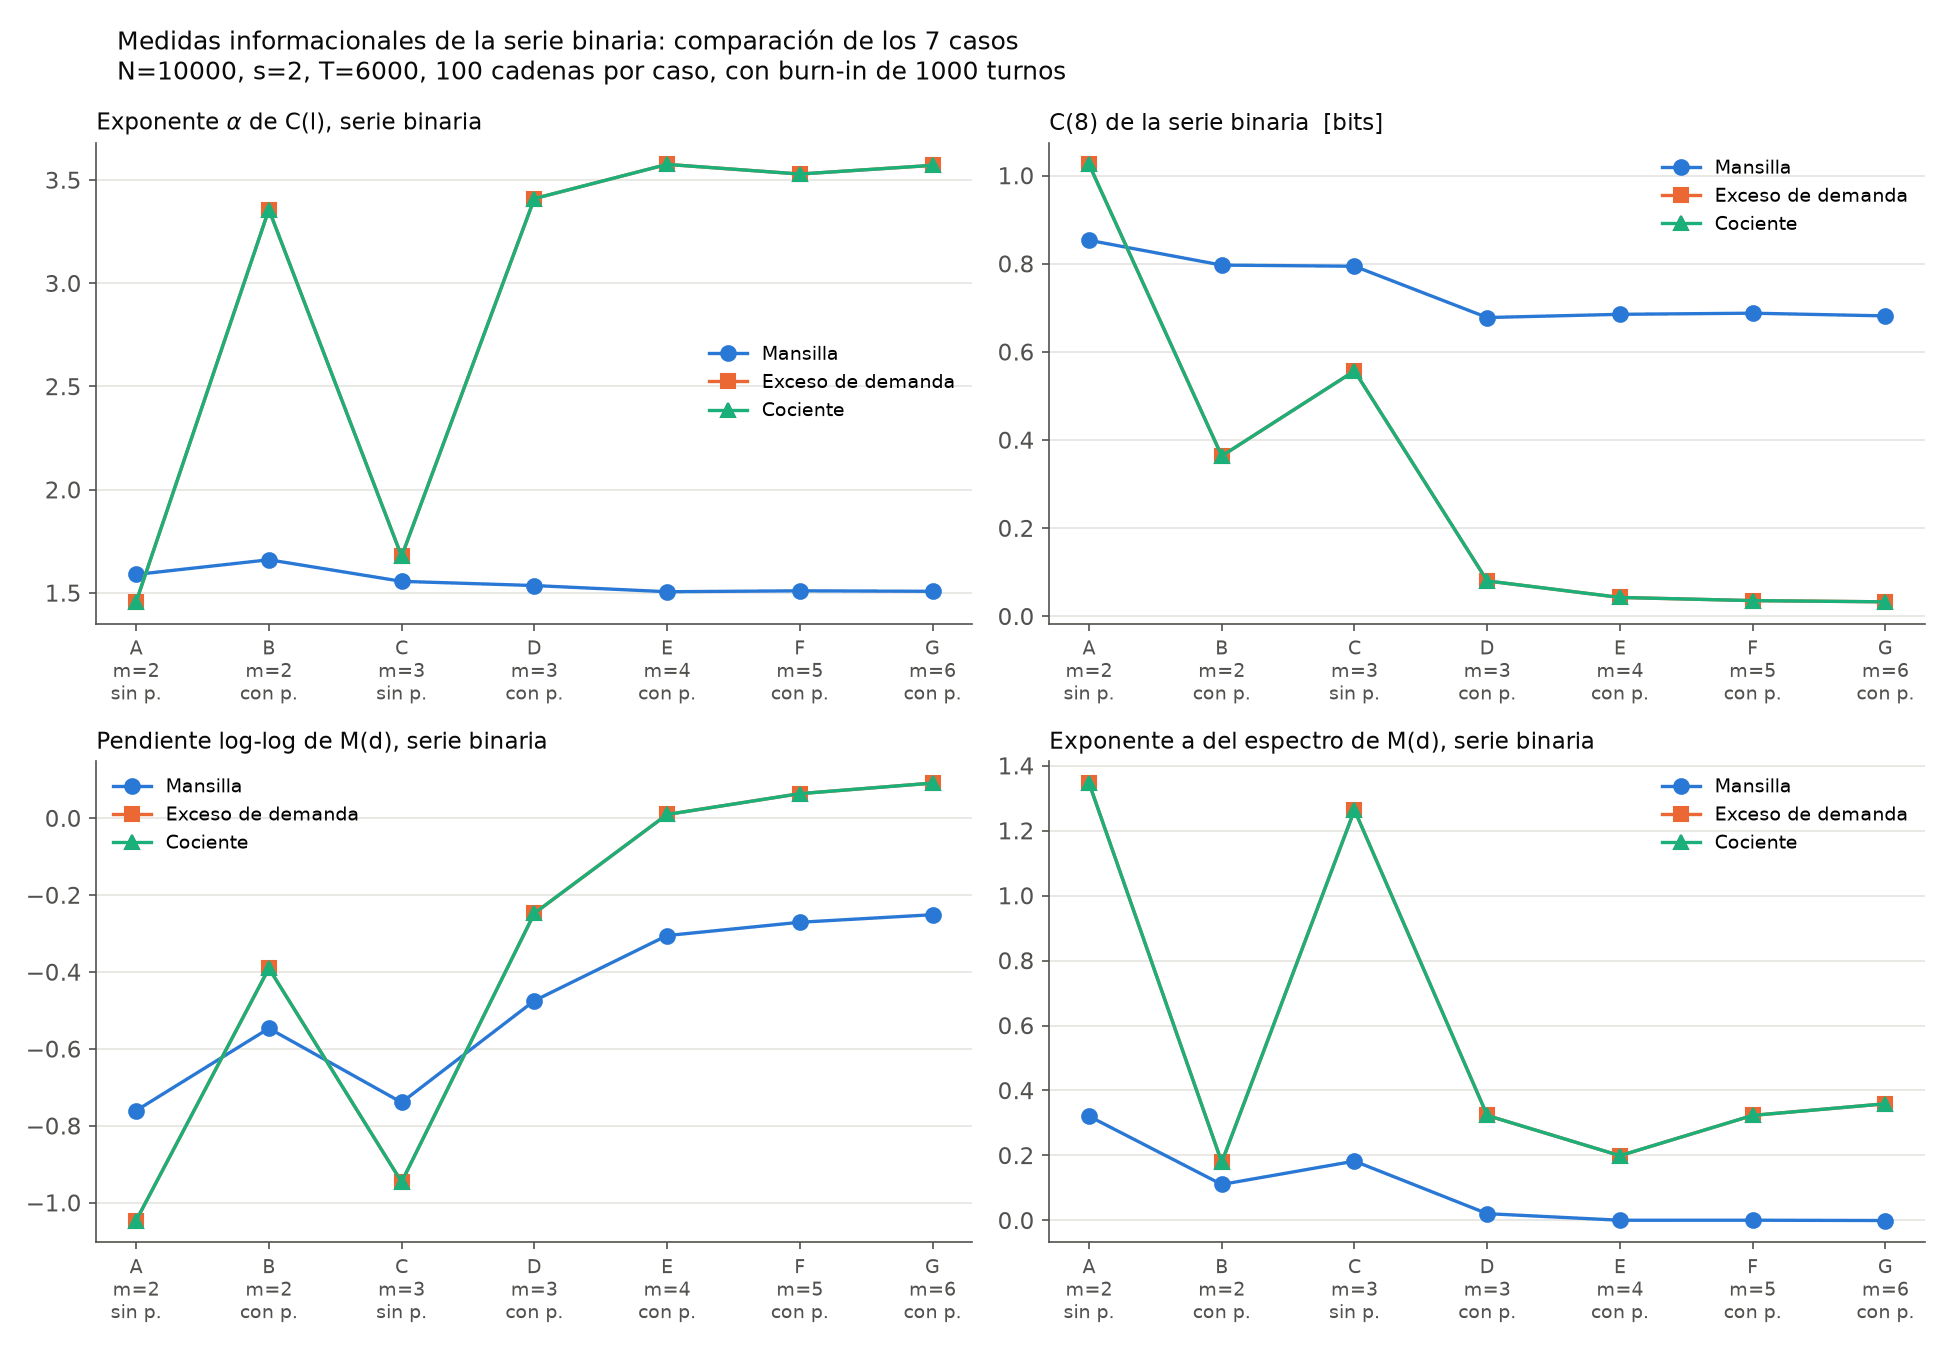
\includegraphics[width=0.95\textwidth]{figuras/Fase9_comparacion_medidas_informacionales_N10000_s2_T6000_regla_nueva.png}
\caption{Medidas informacionales de la serie binaria en los 7 casos, con burn-in.}
\end{figure}

\subsubsection*{Observaciones}
\begin{itemize}
\item \textbf{Colas anchas y agrupamiento de la volatilidad aparecen con puntaje y $m=3$, 4 y 5} (casos D, E y F). La curtosis crece de D a F y llega a 3.65 con el precio de Mansilla en F; el exponente de la cola baja hasta 3.5. La autocorrelación de $|r_t|$ con retardo 1 vale de 0.13 a 0.33.
\item \textbf{El decaimiento de la autocorrelación} sigue bien una ley de potencia en E ($R^2=0.55$ a 0.67, exponente 1.03 a 1.16) y en F ($R^2=0.80$ a 0.83, exponente 0.55 a 0.61). En D el $R^2$ es menor que 0.06, así que ahí el exponente no describe la curva.
\item \textbf{Sin puntaje (A, C) y con $m=6$ (G)} los rendimientos se parecen a una normal: curtosis cercana a 0 o negativa, exponente de cola de 6.2 a 7.4, y autocorrelación de $|r_t|$ casi nula en los acumulados. El caso B ($m=2$ con puntaje) también tiene curtosis pequeña.
\item \textbf{En el precio de Mansilla} la autocorrelación de $|r_t|$ con retardo 1 es de 0.2 aun sin puntaje. Mi interpretación, no comprobada, es que $r_t$ y $r_{t+1}$ comparten el valor $p_t$.
\item \textbf{Ráfagas de volatilidad.} En la cadena destacada del caso F la volatilidad sube en ráfagas separadas por unos 730 turnos, y en ellas $f_2$ oscila más. El número coincide con $3^6=729$. Lo vi a ojo en la gráfica; no lo medí.
\item \textbf{Fracción de abstención:} en promedio vale 0.333 en los siete casos. Sus fluctuaciones son mayores con puntaje (desviación de 0.062 en B contra 0.005 sin puntaje) y bajan al crecer $m$.
\item \textbf{Serie binaria de Mansilla:} $\alpha\approx 1.5$ a 1.66 en todos los casos, como con $N=101$. \textbf{Acumulados:} $\alpha\approx 1.46$ y 1.68 sin puntaje, y 3.36 a 3.58 con puntaje, valores dentro del intervalo 2.1 a 3.8 del artículo de Mansilla solo con puntaje.
\item \textbf{$M(d)$ de la serie binaria de los acumulados:} sin puntaje decae con pendiente cercana a $-1$ ($R^2=0.82$ y 0.88). Con puntaje $M(1)$ es muy pequeña y el máximo aparece en $d=m+1$ (3, 4, 5 y 6 en B, D, E y F) y en $d=81$ en G.
\item \textbf{Ráfagas en el precio de Mansilla.} En D, E y F las 100 cadenas muestran ráfagas regulares de precios extremos. En E se ven unas 24 en 6000 turnos (separación de unos 250 turnos, cerca de $3^5=243$) y en F unas 8 (cerca de $3^6=729$). En G solo hay una ráfaga al inicio. Visto a ojo, sin medir.
\item \textbf{Precios acumulados:} con $N=10000$ el recorrido mediano es menor que con $N=101$ sin puntaje (A y C) y mayor con puntaje (B y D) (tablas~\ref{tab:f9n101} y~\ref{tab:f9n10000}). En A, B, C y D la cadena destacada sigue casi en línea recta; en E, F y G sube con tramos planos y saltos. No se ven burbujas.
\end{itemize}

Las 49 gráficas por caso están en el apéndice~\ref{ap:f9n10000}, y los resultados de la codificación ternaria en el apéndice~\ref{ap:ternaria}.

\section{Fase 11: búsqueda de la fase gaseosa}
Con $m=2$, $s=2$ y tres decisiones hay $K^{K^m}=3^9=19683$ estrategias posibles. Se buscó la fase gaseosa aumentando $N$ por encima de ese número, hasta un millón de agentes ($T=6000$, con puntaje, regla nueva). El criterio que elegiste: la fase gaseosa se da por encontrada si desaparecen los picos de $M(d)$ en $d=27$, 54 y 81. Para medirlo se usa el \textbf{contraste}, $M(d_0)$ dividido entre la mediana de sus 14 vecinos; 1 significa que no hay pico, y el umbral acordado fue 2. La corrida duró 475 minutos; los datos se guardaron comprimidos (un \texttt{.npz} por $N$, 29 MB en total).

\begin{table}[H]
\centering
\scriptsize
\setlength{\tabcolsep}{3.5pt}
\caption{Fase 11, $m=2$, $s=2$, con puntaje, $T=6000$, 100 cadenas. $N s/\text{estr.}$ es $N\cdot s$ entre las 19683 estrategias. ``Azar'' es la tasa de éxito de agentes que eligen al azar con ese $N$. Contraste: $M(d_0)$ entre la mediana de sus 14 vecinos. ``Frac. esp.'' es la fracción de la potencia del espectro de $M(d)$ en sus 3 picos más altos. $C(1)$ a $C(3)$ son menores que $10^{-5}$ en todos los $N$.}\label{tab:f11}
\begin{adjustbox}{max width=\textwidth}
\begin{tabular}{rrrrrrrrrrcrrrr}
\toprule
$N$ & $\gamma$ & $Ns/$estr. & Éxito & Azar & $M(1)$ & $M(2)$ & $M(3)$ & $M(4)$ & $d_{\max}$ & Contraste 27/54/81 & Frac. esp. & $C(4)$ & $C(6)$ & Vacías \\
\midrule
101 & $8.91\times10^{-2}$ & 0.01 & 0.2760 & 0.2852 & $9.45\times10^{-7}$ & $1.32\times10^{-6}$ & $1.88\times10^{-2}$ & $4.28\times10^{-3}$ & 3 & 2.9 / 2.3 / 2.3 & 0.167 & 0.120 & 0.608 & 0 \\
1\,001 & $8.99\times10^{-3}$ & 0.10 & 0.2756 & 0.3179 & $6.02\times10^{-7}$ & $6.47\times10^{-7}$ & $3.56\times10^{-2}$ & $1.12\times10^{-2}$ & 3 & 10.1 / 9.3 / 9.3 & 0.205 & 0.264 & 1.235 & 0 \\
5\,000 & $1.80\times10^{-3}$ & 0.51 & 0.2772 & 0.3264 & $7.04\times10^{-7}$ & $7.09\times10^{-7}$ & $3.39\times10^{-2}$ & $1.02\times10^{-2}$ & 3 & 8.6 / 8.7 / 8.8 & 0.216 & 0.260 & 1.214 & 0 \\
9\,842 & $9.14\times10^{-4}$ & 1.00 & 0.2778 & 0.3284 & $5.88\times10^{-7}$ & $7.50\times10^{-7}$ & $3.40\times10^{-2}$ & $9.37\times10^{-3}$ & 3 & 8.4 / 8.4 / 8.5 & 0.213 & 0.257 & 1.226 & 0 \\
19\,684 & $4.57\times10^{-4}$ & 2.00 & 0.2781 & 0.3298 & $6.13\times10^{-7}$ & $6.92\times10^{-7}$ & $3.24\times10^{-2}$ & $1.02\times10^{-2}$ & 3 & 10.3 / 8.7 / 9.0 & 0.221 & 0.261 & 1.223 & 0 \\
40\,000 & $2.25\times10^{-4}$ & 4.06 & 0.2778 & 0.3309 & $5.66\times10^{-7}$ & $6.97\times10^{-7}$ & $3.22\times10^{-2}$ & $9.68\times10^{-3}$ & 3 & 9.1 / 8.5 / 8.1 & 0.218 & 0.251 & 1.218 & 0 \\
100\,000 & $9.00\times10^{-5}$ & 10.16 & 0.2778 & 0.3318 & $5.78\times10^{-7}$ & $6.91\times10^{-7}$ & $3.22\times10^{-2}$ & $9.14\times10^{-3}$ & 3 & 9.5 / 9.3 / 8.8 & 0.213 & 0.260 & 1.218 & 0 \\
400\,000 & $2.25\times10^{-5}$ & 40.64 & 0.2780 & 0.3326 & $5.38\times10^{-7}$ & $6.53\times10^{-7}$ & $3.05\times10^{-2}$ & $8.55\times10^{-3}$ & 3 & 8.8 / 8.4 / 8.3 & 0.207 & 0.244 & 1.157 & 0 \\
1\,000\,000 & $9.00\times10^{-6}$ & 101.61 & 0.2783 & 0.3328 & $5.87\times10^{-7}$ & $6.43\times10^{-7}$ & $3.32\times10^{-2}$ & $1.02\times10^{-2}$ & 3 & 8.9 / 8.5 / 8.1 & 0.215 & 0.252 & 1.205 & 0 \\
\bottomrule
\end{tabular}
\end{adjustbox}
\end{table}


\begin{figure}[H]
\centering
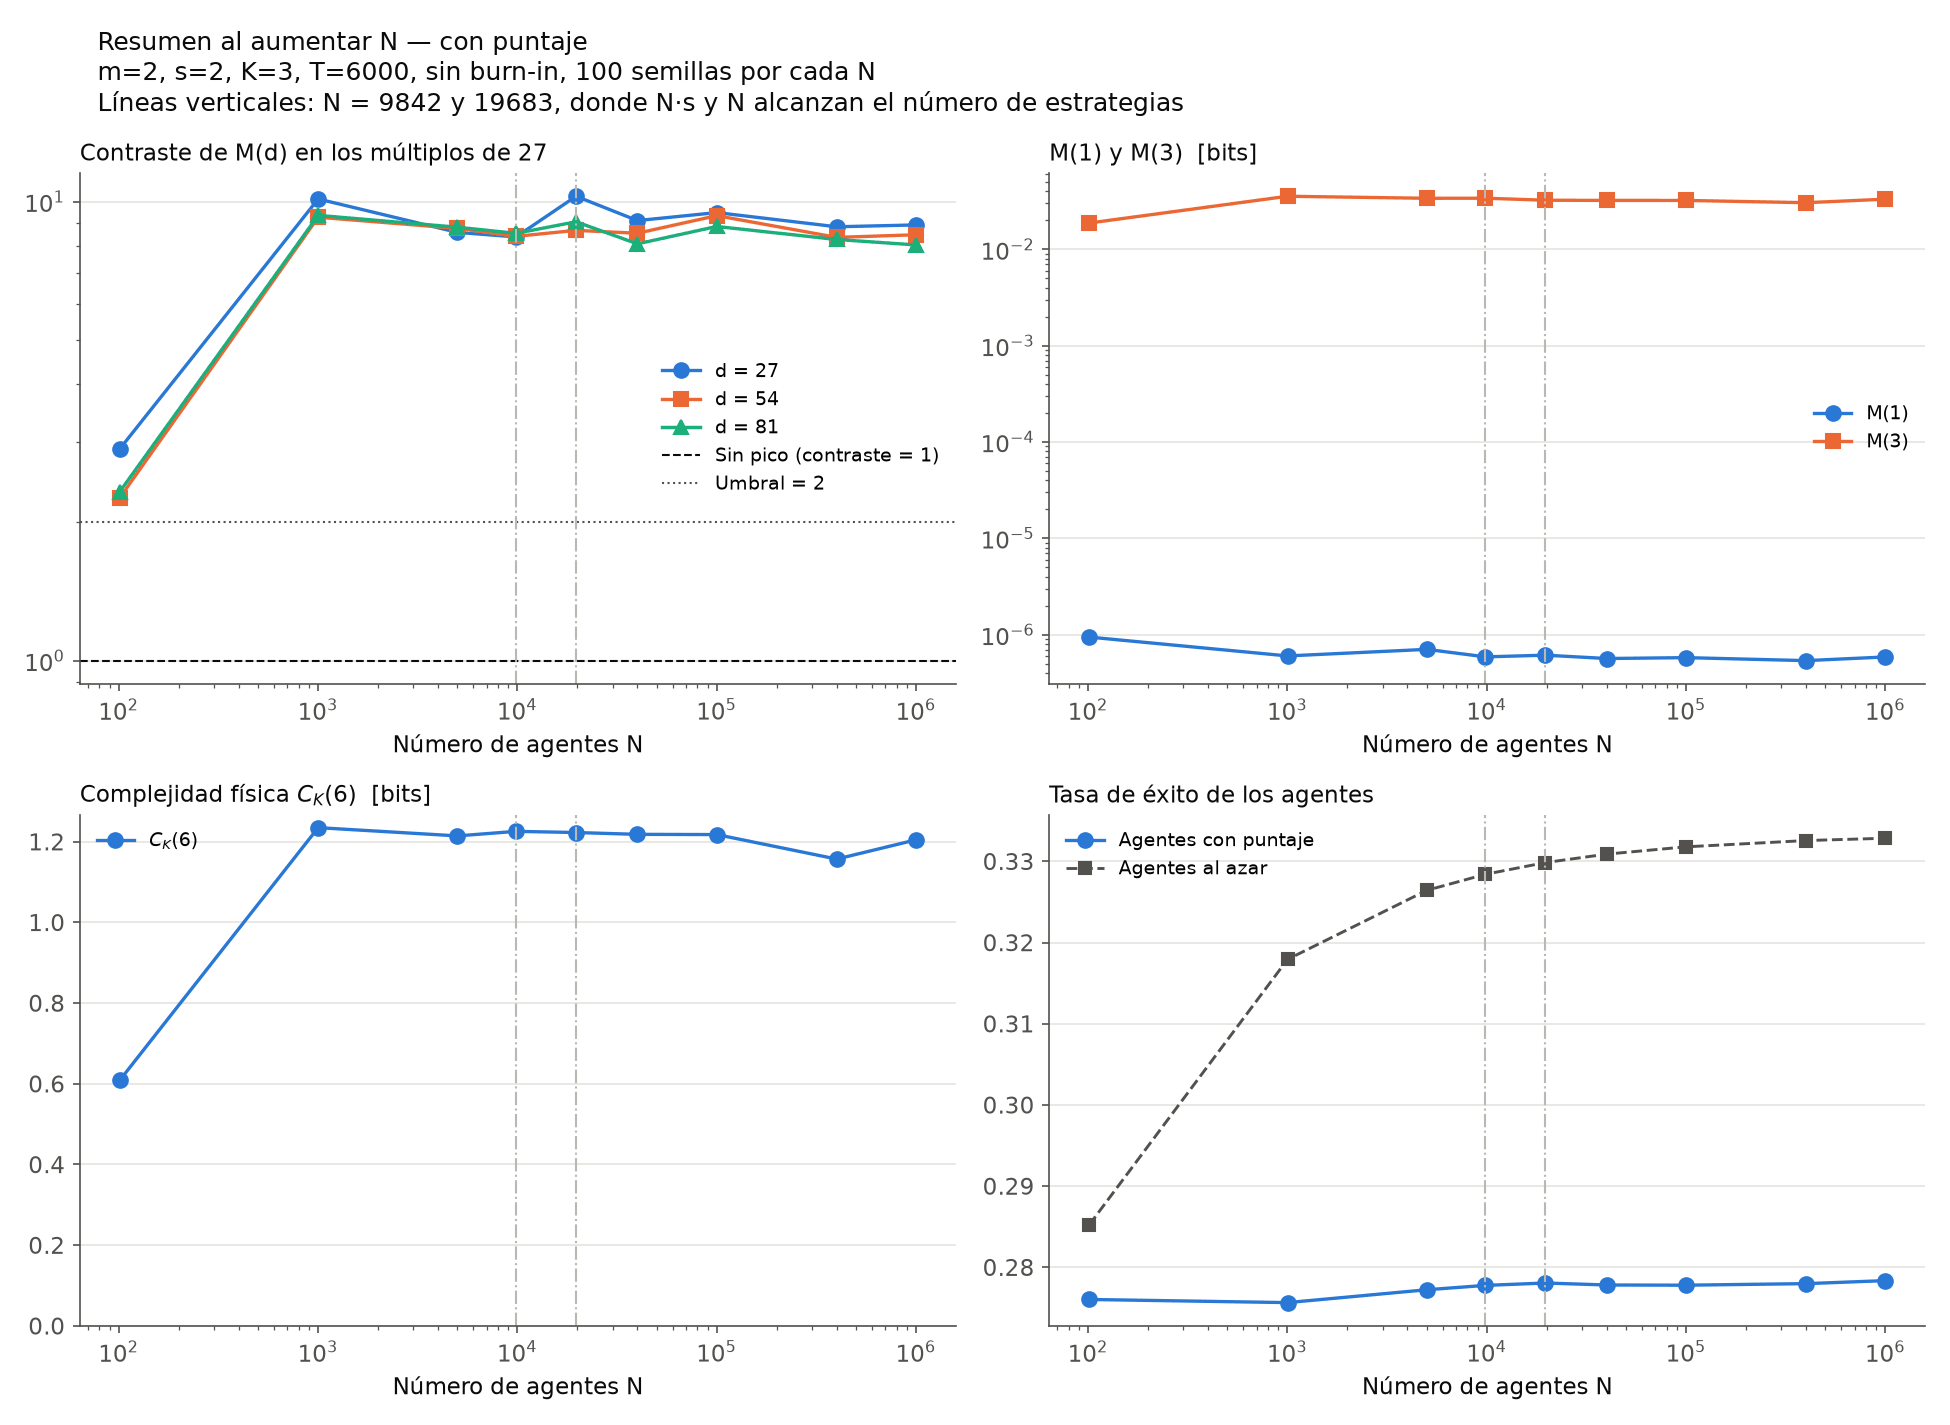
\includegraphics[width=0.92\textwidth]{figuras/Fase11_resumen_con_puntaje_m2_s2_T6000_N101-a-1000000_9valores.png}
\caption{Fase 11, resumen contra $N$. Las líneas verticales marcan $N=9842$ y $N=19683$, donde $N\cdot s$ y $N$ alcanzan el número de estrategias.}
\end{figure}
\begin{figure}[H]
\centering
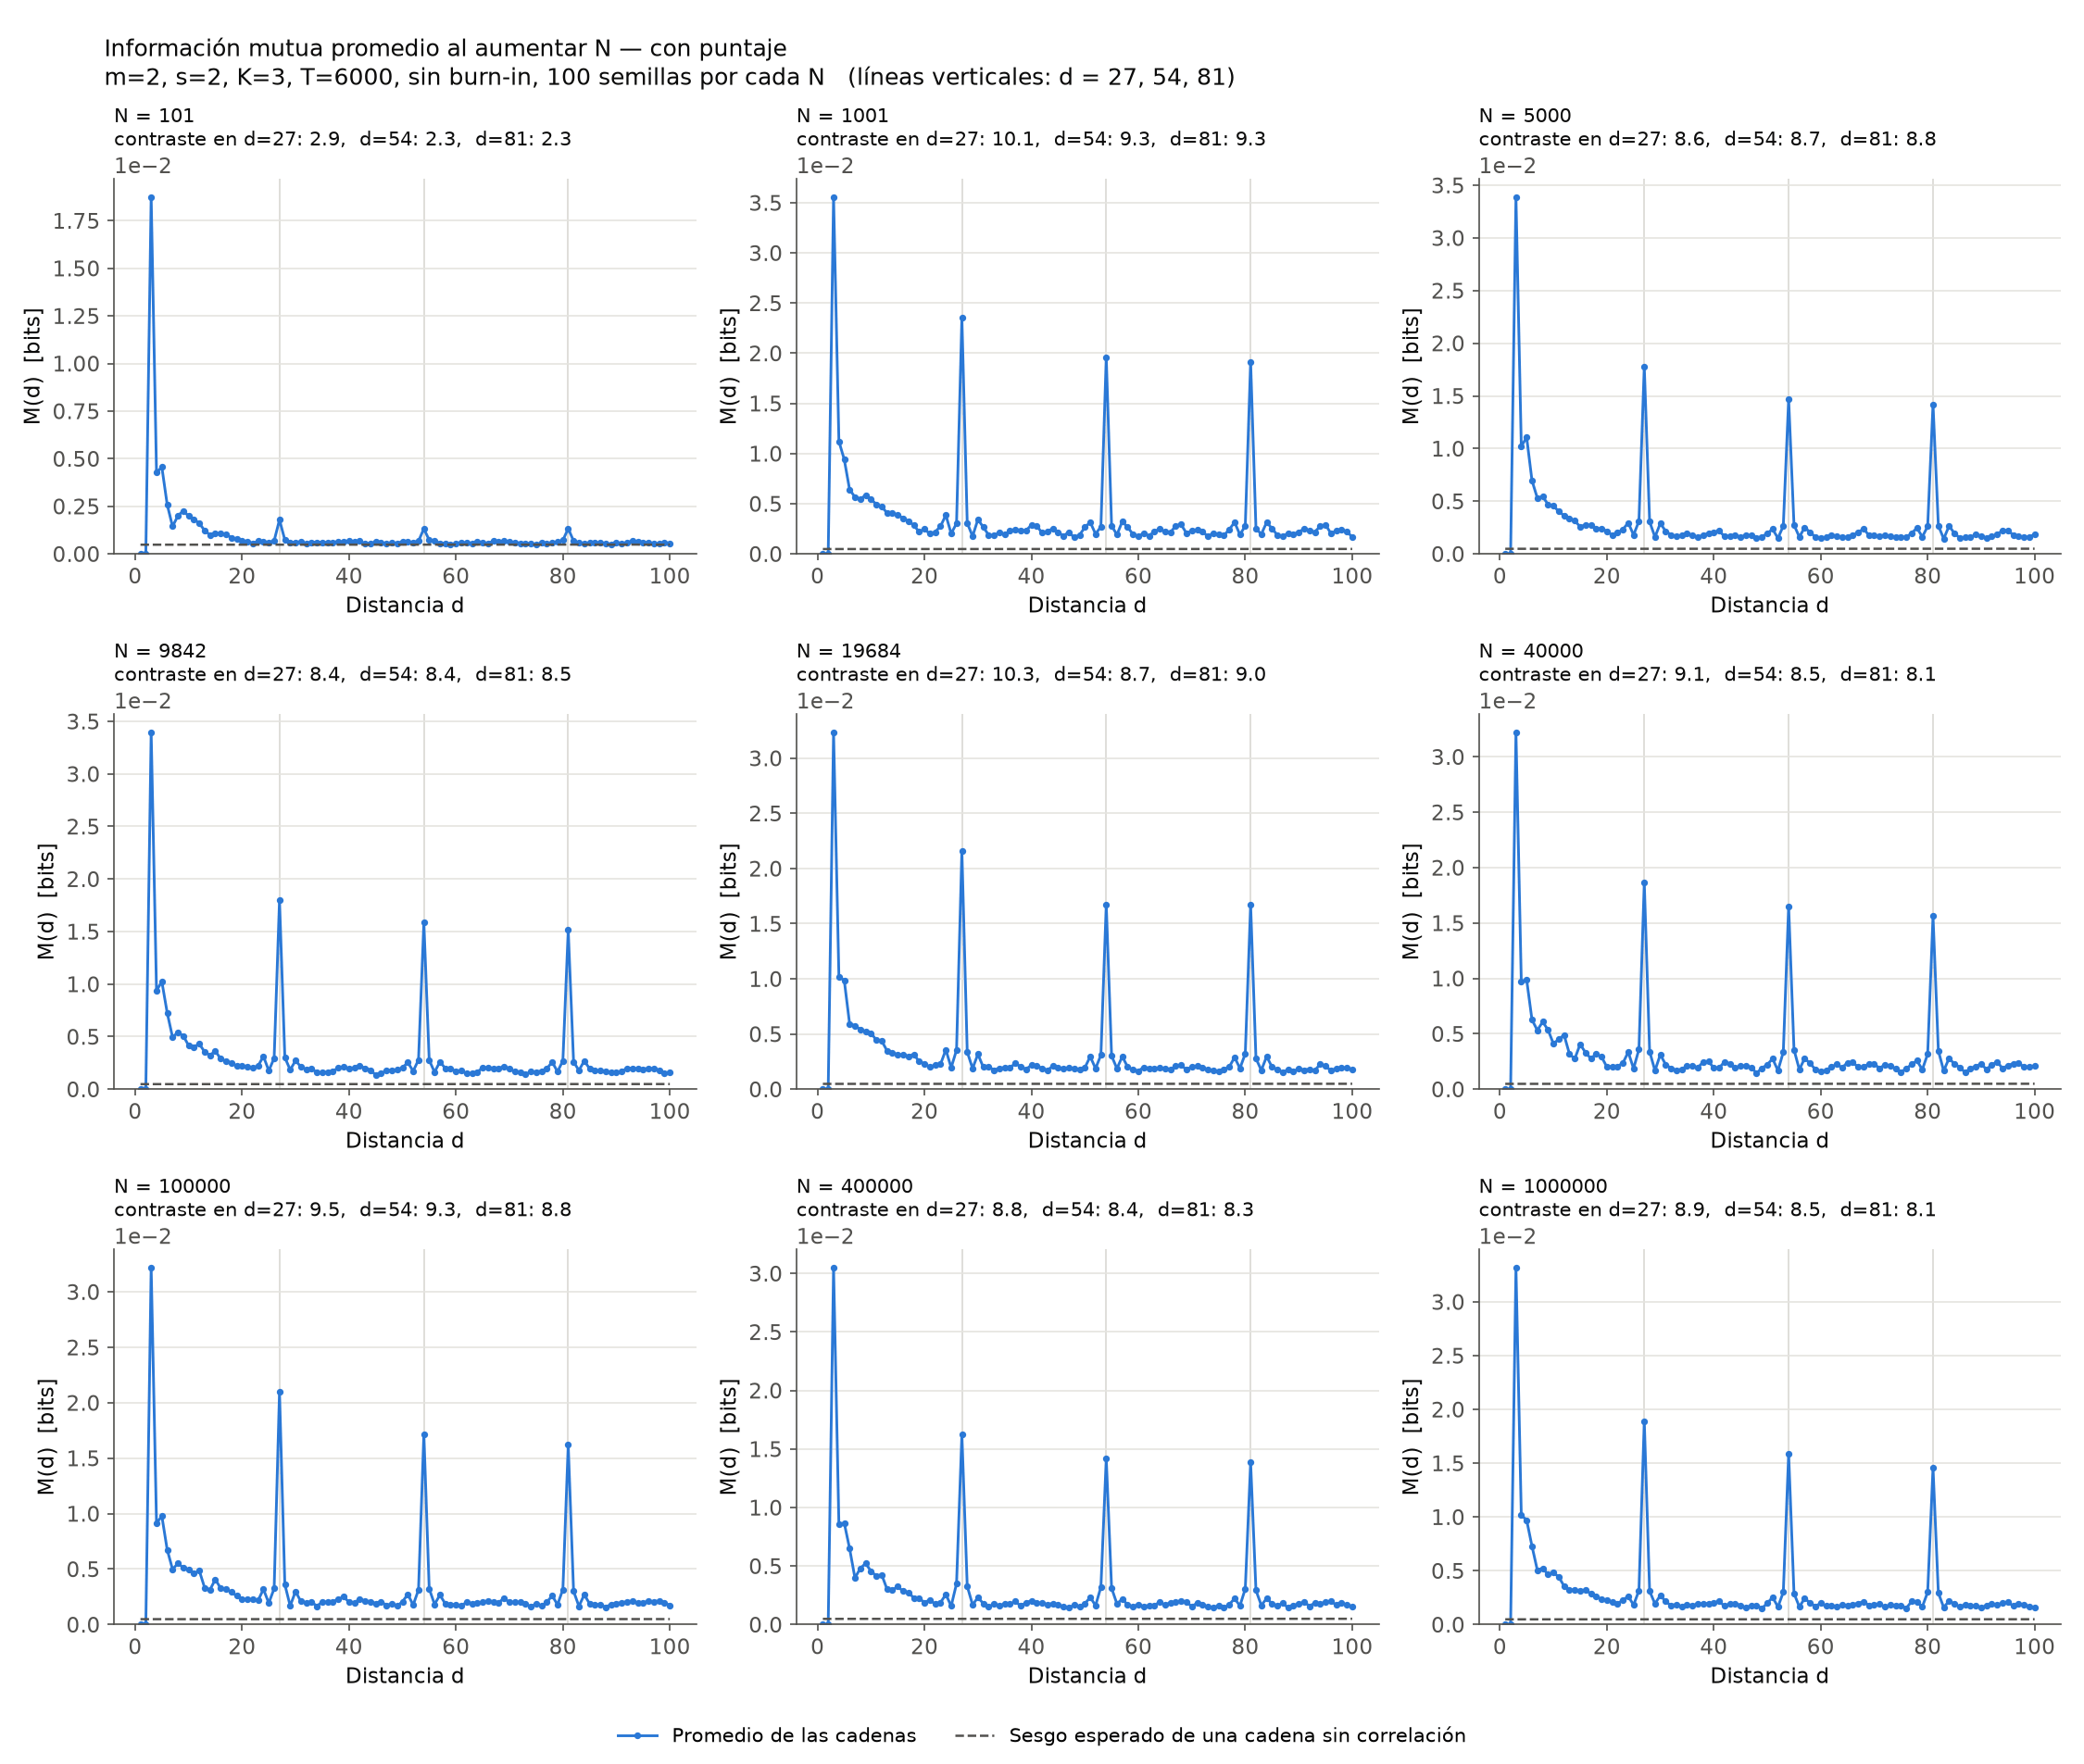
\includegraphics[width=0.92\textwidth]{figuras/Fase11_Md_con_puntaje_m2_s2_T6000_N101-a-1000000_9valores.png}
\caption{Fase 11, $M(d)$ promedio para los 9 valores de $N$.}
\end{figure}
\begin{figure}[H]
\centering
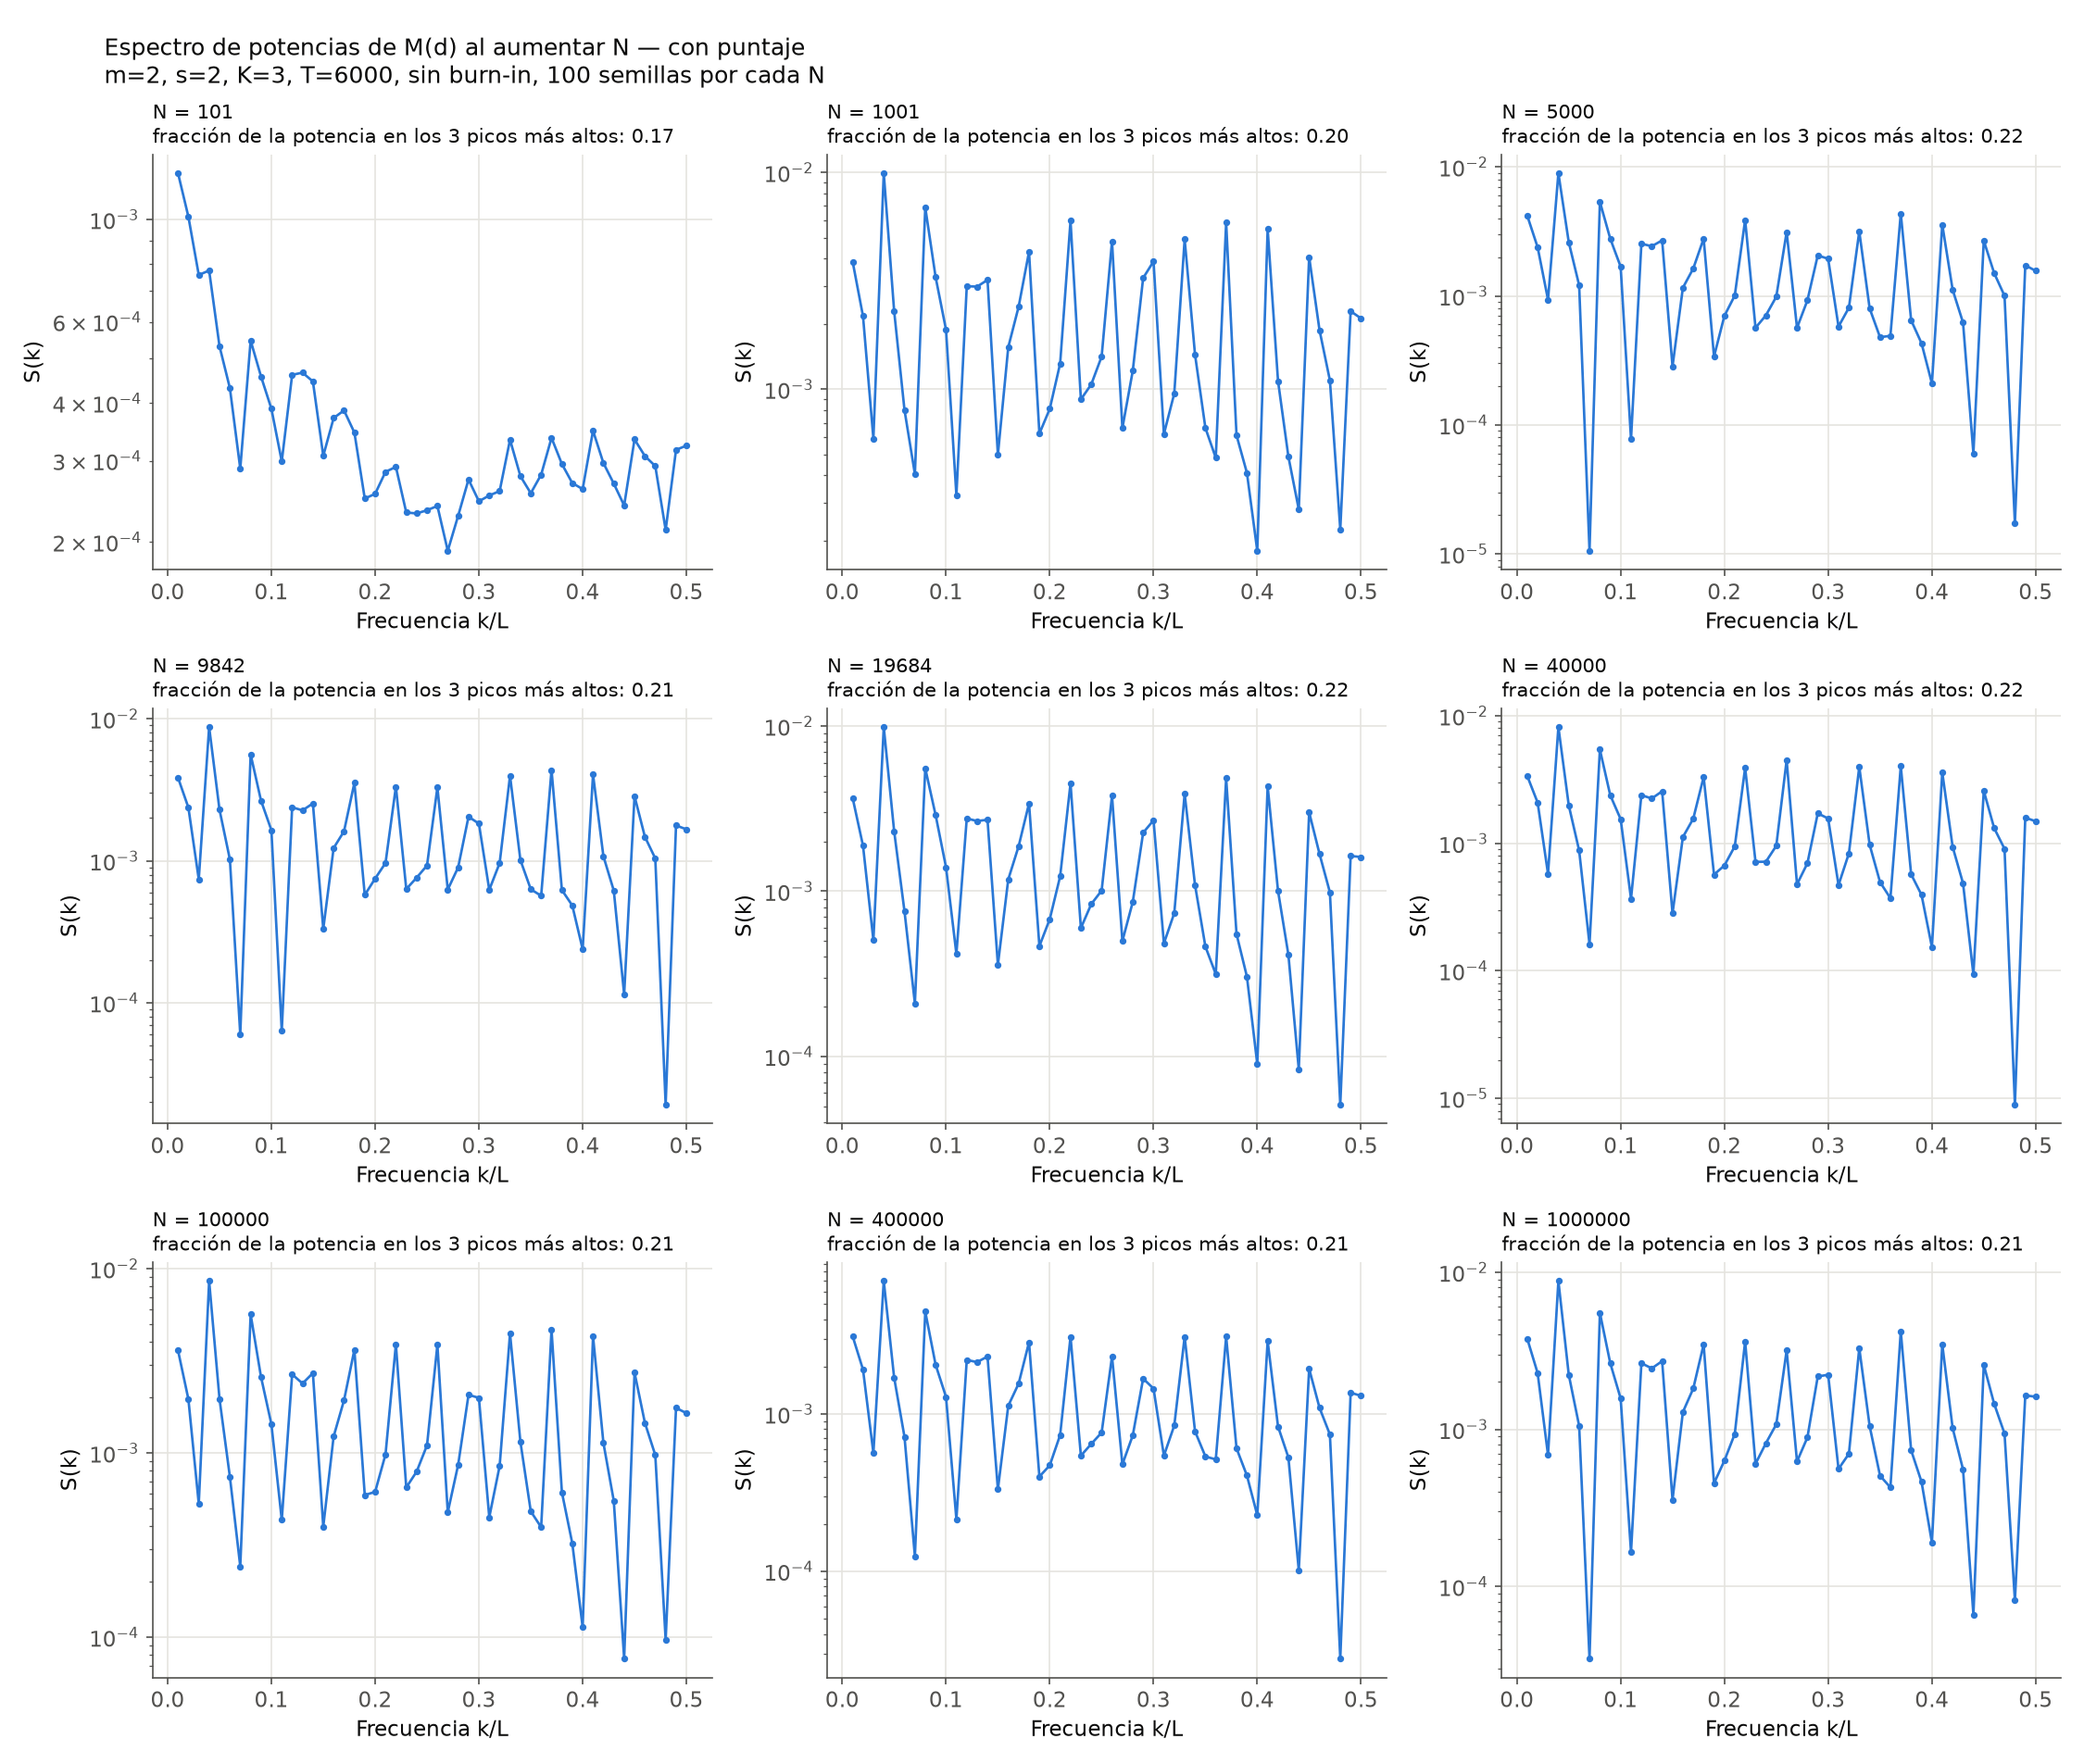
\includegraphics[width=0.92\textwidth]{figuras/Fase11_espectro_con_puntaje_m2_s2_T6000_N101-a-1000000_9valores.png}
\caption{Fase 11, espectro de potencias de $M(d)$ para los 9 valores de $N$.}
\end{figure}
\begin{figure}[H]
\centering
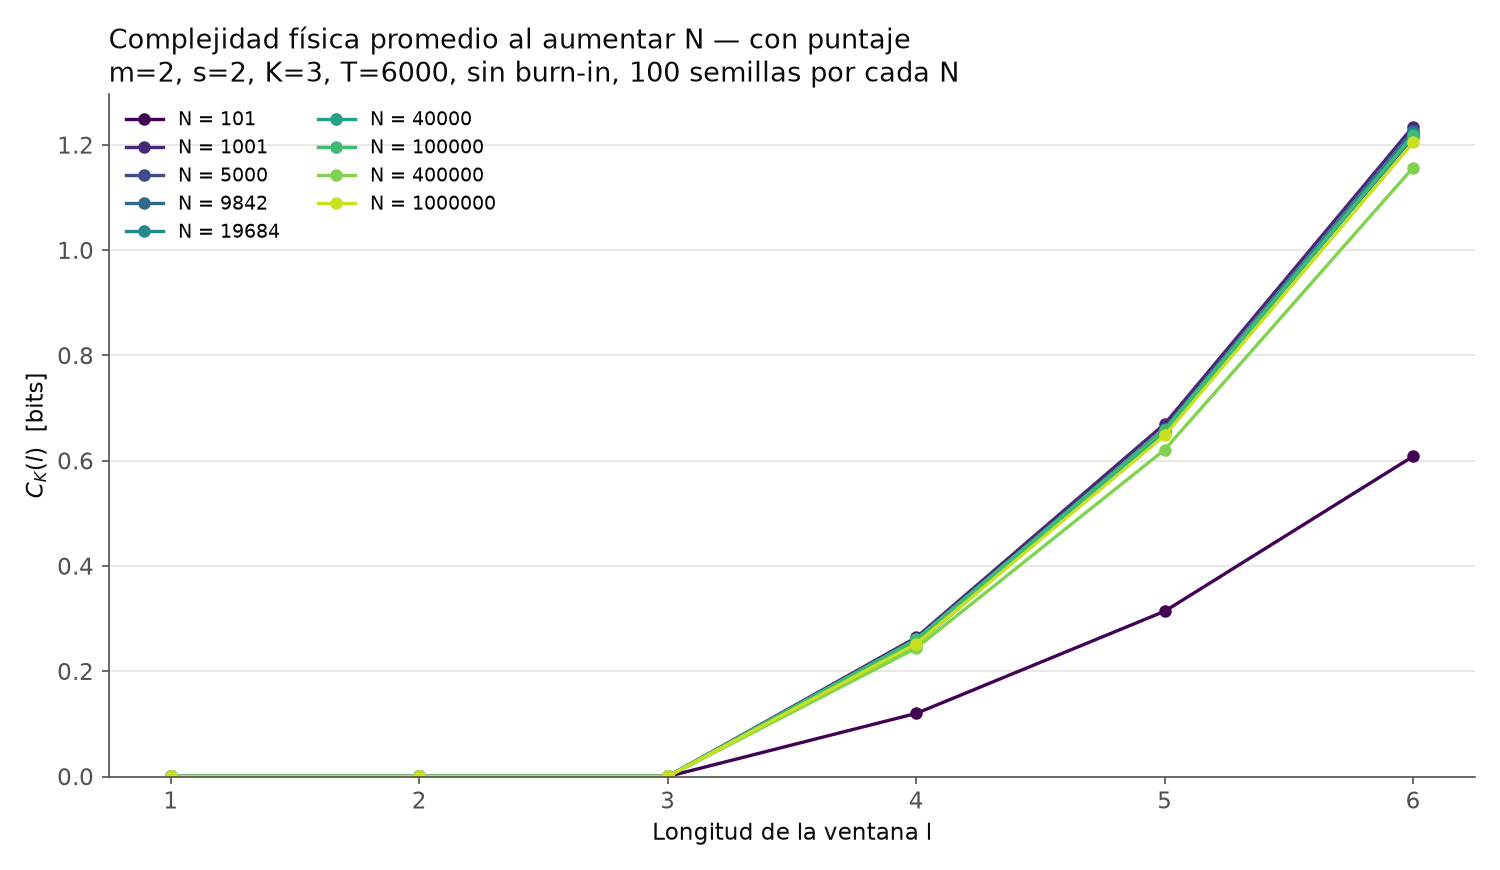
\includegraphics[width=0.6\textwidth]{figuras/Fase11_CK_con_puntaje_m2_s2_T6000_N101-a-1000000_9valores.png}
\caption{Fase 11, $C(l)$ promedio.}
\end{figure}

\subsubsection*{Observaciones}
\begin{itemize}
\item \textbf{No apareció la fase gaseosa.} Los picos en $d=27$, 54 y 81 siguen en los 9 valores de $N$, con contraste de 8 a 10 desde $N=1001$ hasta un millón.
\item \textbf{Las curvas casi no cambian desde $N=1001$.} Pasar el número de estrategias posibles no altera nada: las curvas de 9842, 19684 y un millón son prácticamente iguales.
\item \textbf{Los picos son más débiles con pocos agentes}, no con muchos: el único caso distinto es $N=101$, con contraste de 2.3 a 2.9.
\item \textbf{$M(1)$ y $M(2)$ valen casi cero} (unos $6\times10^{-7}$ bits), unas 800 veces menos que una serie al azar con $T=6000$ ($4.8\times10^{-4}$). El primer valor grande es $M(3)$. $C(l)$ es prácticamente cero para $l\le 3$.
\item \textbf{La periodicidad es una tendencia, no una repetición exacta:} el resultado se repite 27 turnos después en el 40\,\% de los turnos (al azar sería el 33\,\%; a 26 turnos, el 35\,\%).
\item \textbf{Los agentes ganan menos que al azar} en todos los $N$ (0.278 contra 0.333 con un millón).
\item \textbf{Interpretación mía, sin comprobar:} $27=3\times 3^2=K\cdot K^m$. En el juego binario la literatura describe una dinámica de periodo $2\cdot 2^m$ justamente cuando hay muchos agentes, así que esta periodicidad podría ser la marca de esa zona y no algo que desaparezca al agregar más agentes. Conviene consultarlo con el Dr. Mansilla.
\end{itemize}

\section{Fase 12: ajuste de la función de Hill}
Encargo del Dr. Mansilla: calcular $M(d)$ para cinco combinaciones de $m$ y $s$, todas con puntaje, $K=3$, $N=101$ y $T=60000$, y ajustar a $y=\log_{10}M(d)$ contra $x=\log_{10}d$ la función de Hill
\begin{equation*}
H(x)=A+\frac{B}{1+(x/C)^{\alpha}},
\end{equation*}
con el script \texttt{ajuste\_hill.py} del Dr. Mansilla, copiado sin cambios y con sus valores por defecto (30 arranques, semilla 12345, $\alpha$ entre 0.01 y 100). En palabras: $A$ es el nivel de $\log_{10}M$ para $d$ grande, $A+B$ el nivel en $d=1$, $C$ es el $\log_{10}d$ donde ocurre la mitad de la caída ($d_C=10^C$), y $\alpha$ mide qué tan brusca es. Se hicieron \textbf{dos ajustes} por caso, como pediste: con todos los $d$, y con $d\ge m+1$. También se reporta la recta log-log con todos los $d$.

Con $s=0$ los agentes no tienen estrategias y eligen al azar, así que $m$ no interviene: $m=1,s=0$ y $m=2,s=0$ son la misma simulación, y solo cambia el ajuste desde $d\ge m+1$. Con $s=1$ cada agente tiene una sola estrategia fija y el puntaje no tiene efecto.

\begin{table}[H]
\centering
\footnotesize
\setlength{\tabcolsep}{3.5pt}
\caption{Fase 12, $K=3$, $N=101$, $T=60000$, 100 cadenas, regla vieja. Frecuencias de los símbolos 0, 1 y 2 en la serie de ganadores. La tasa de éxito de agentes al azar es 0.2852. No hubo turnos con una opción vacía en ningún caso.}\label{tab:f12casos}
\begin{adjustbox}{max width=\textwidth}
\begin{tabular}{llllrrrrr}
\toprule
Caso & $\gamma$ & Frecuencias (0, 1, 2) & Éxito & $M(1)$ & $M(2)$ & $M(3)$ & $M_{\max}$ & $d_{\max}$ \\
\midrule
$s=0$ (azar) & -- & 0.3334, 0.3332, 0.3335 & no se mide & $5.25\times10^{-5}$ & $5.07\times10^{-5}$ & $4.67\times10^{-5}$ & $5.78\times10^{-5}$ & 13 \\
$m=1$, $s=1$ & 0.0297 & 0.4190, 0.3277, 0.2533 & 0.2836 & 0.405 & 0.369 & 0.344 & 0.405 & 1 \\
$m=2$, $s=1$ & 0.0891 & 0.3039, 0.3796, 0.3165 & 0.2859 & 0.470 & 0.542 & 0.535 & 0.609 & 60 \\
$m=2$, $s=2$ & 0.0891 & 0.3333, 0.3333, 0.3333 & 0.2761 & $7.94\times10^{-9}$ & $1.07\times10^{-8}$ & $1.83\times10^{-2}$ & $1.83\times10^{-2}$ & 3 \\
\bottomrule
\end{tabular}
\end{adjustbox}
\end{table}


\begin{table}[H]
\centering
\footnotesize
\setlength{\tabcolsep}{3.5pt}
\caption{Fase 12: ajustes de Hill $H(x)=A+B/[1+(x/C)^\alpha]$ con $x=\log_{10}d$ y $y=\log_{10}M(d)$; $d_C=10^C$. ``Conv.'' es cuántos de los 30 arranques convergieron. Avisos del script: ``límite'' si $C$ o $\alpha$ quedó junto a un límite de búsqueda; ``débil'' si los parámetros están mal determinados. Los dos casos con $s=0$ usan los mismos datos.}\label{tab:f12hill}
\begin{adjustbox}{max width=\textwidth}
\begin{tabular}{rrlrrrrrrrrrl}
\toprule
$m$ & $s$ & Rango & $n$ & $A$ & $B$ & $C$ & $d_C$ & $\alpha$ & $R^2$ & RMSE & Conv. & Avisos \\
\midrule
1 & 0 & todos & 100 & $-$4.329 & 0.049 & 0.450 & 2.82 & 1.38 & 0.0292 & 0.0322 & 24/30 & -- \\
1 & 0 & $d\ge2$ & 99 & $-$4.322 & $6.29\times10^{8}$ & 0.214 & 1.64 & 70.31 & 0.0068 & 0.0325 & 3/30 & débil \\
1 & 1 & todos & 100 & $-$0.488 & 0.096 & 0.337 & 2.17 & 3.66 & 0.9971 & 0.0006 & 30/30 & -- \\
1 & 1 & $d\ge2$ & 99 & $-$0.488 & 0.062 & 0.445 & 2.79 & 5.69 & 0.9995 & 0.0001 & 30/30 & -- \\
2 & 0 & todos & 100 & $-$4.329 & 0.049 & 0.450 & 2.82 & 1.38 & 0.0292 & 0.0322 & 24/30 & -- \\
2 & 0 & $d\ge3$ & 98 & $-$4.321 & $-$0.553 & 0.456 & 2.86 & 90.41 & 0.0008 & 0.0326 & 2/30 & débil \\
2 & 1 & todos & 100 & $-$0.307 & 0.020 & 0.839 & 6.91 & 10.91 & 0.0133 & 0.0385 & 30/30 & -- \\
2 & 1 & $d\ge3$ & 98 & $-$0.307 & 0.041 & 0.658 & 4.55 & 5.53 & 0.0155 & 0.0386 & 30/30 & -- \\
2 & 2 & todos & 100 & $-$3.653 & $-$4.447 & 0.313 & 2.06 & 87.72 & 0.6779 & 0.4230 & 30/30 & débil \\
2 & 2 & $d\ge3$ & 98 & $-$4.014 & 2.007 & 1.023 & 10.55 & 4.30 & 0.8301 & 0.1761 & 30/30 & -- \\
\bottomrule
\end{tabular}
\end{adjustbox}
\end{table}
\begin{table}[H]
\centering
\small
\setlength{\tabcolsep}{3.5pt}
\caption{Fase 12: recta log-log con todos los $d$ (\texttt{np.polyfit} de grado 1).}\label{tab:f12recta}
\begin{adjustbox}{max width=\textwidth}
\begin{tabular}{rrrr}
\toprule
$m$ & $s$ & Pendiente & $R^2$ \\
\midrule
1 & 0 & $-$0.0115 & 0.0198 \\
1 & 1 & $-$0.0166 & 0.3505 \\
2 & 0 & $-$0.0115 & 0.0198 \\
2 & 1 & $-$0.0076 & 0.0062 \\
2 & 2 & $+$0.0080 & 0.0000 \\
\bottomrule
\end{tabular}
\end{adjustbox}
\end{table}


\begin{figure}[H]
\centering
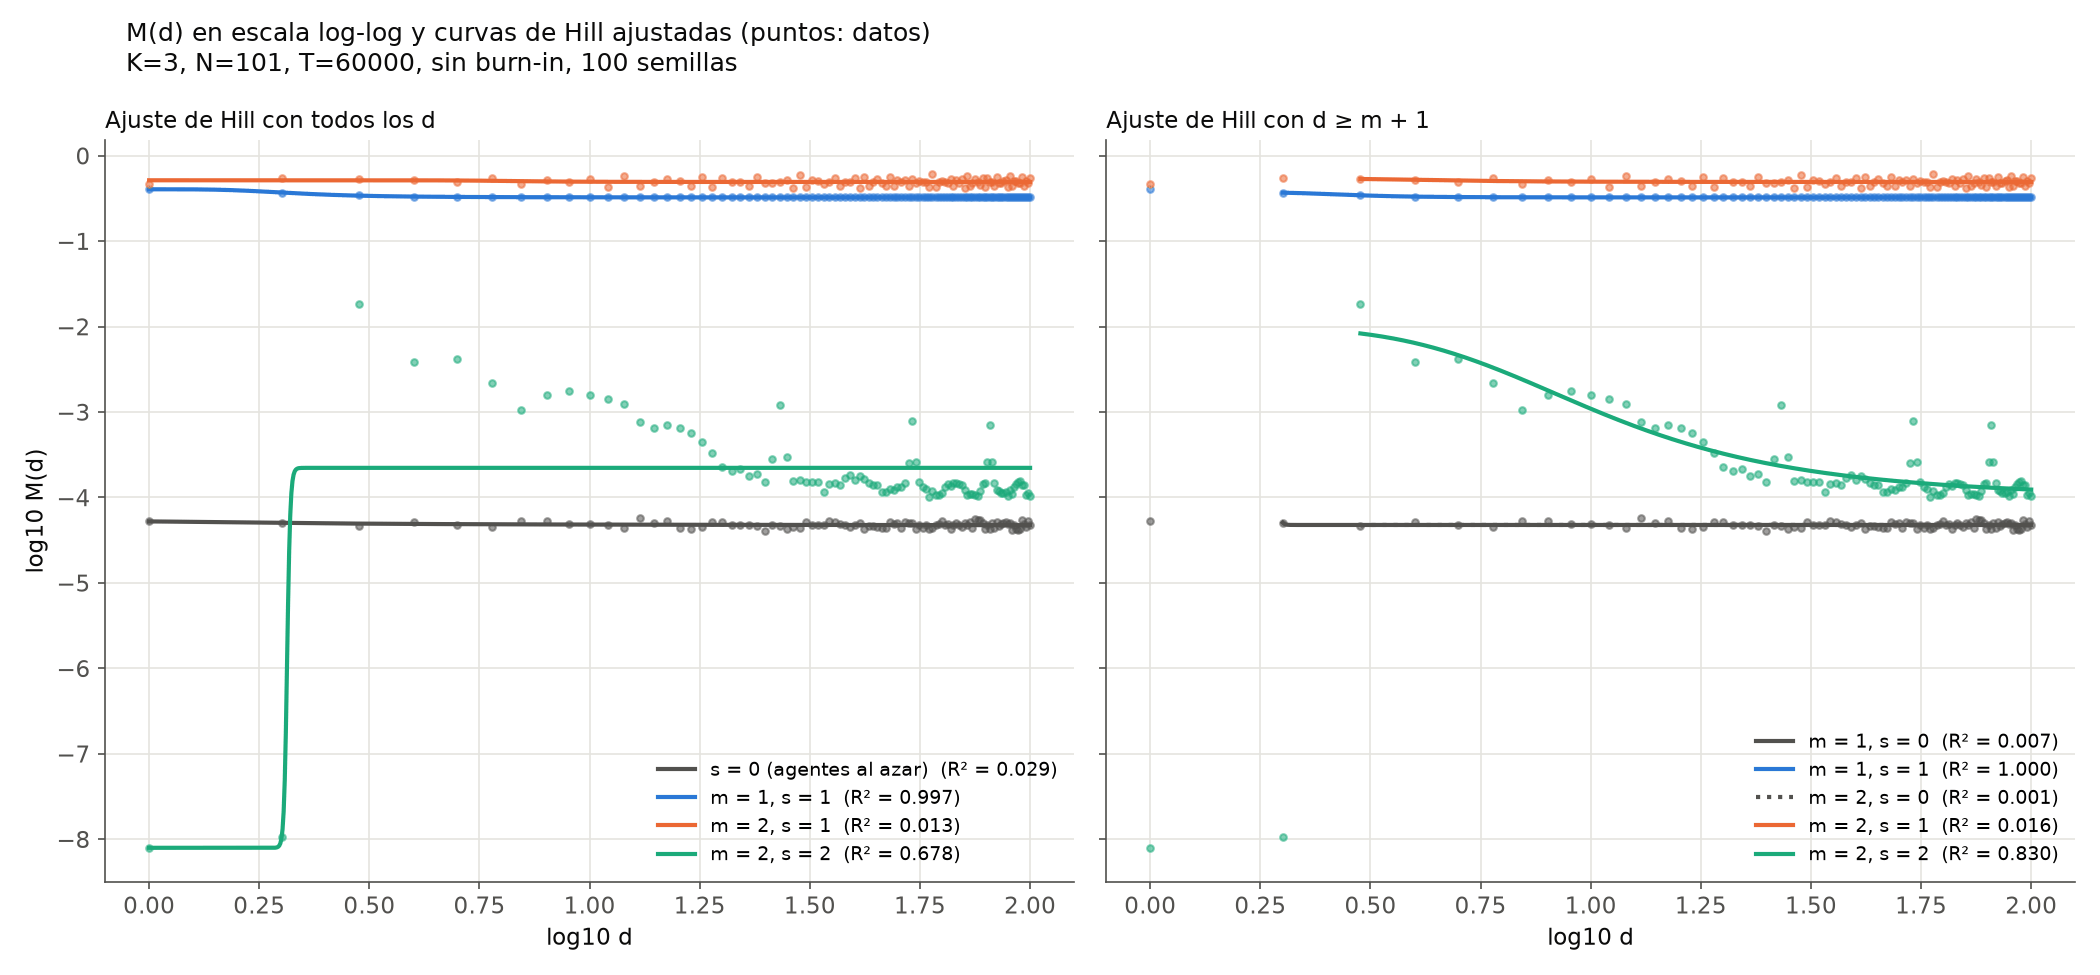
\includegraphics[width=0.92\textwidth]{figuras/Fase12_comparacion_hill_N101_T60000.png}
\caption{Fase 12, comparación de los casos.}
\end{figure}
\begin{figure}[H]
\centering
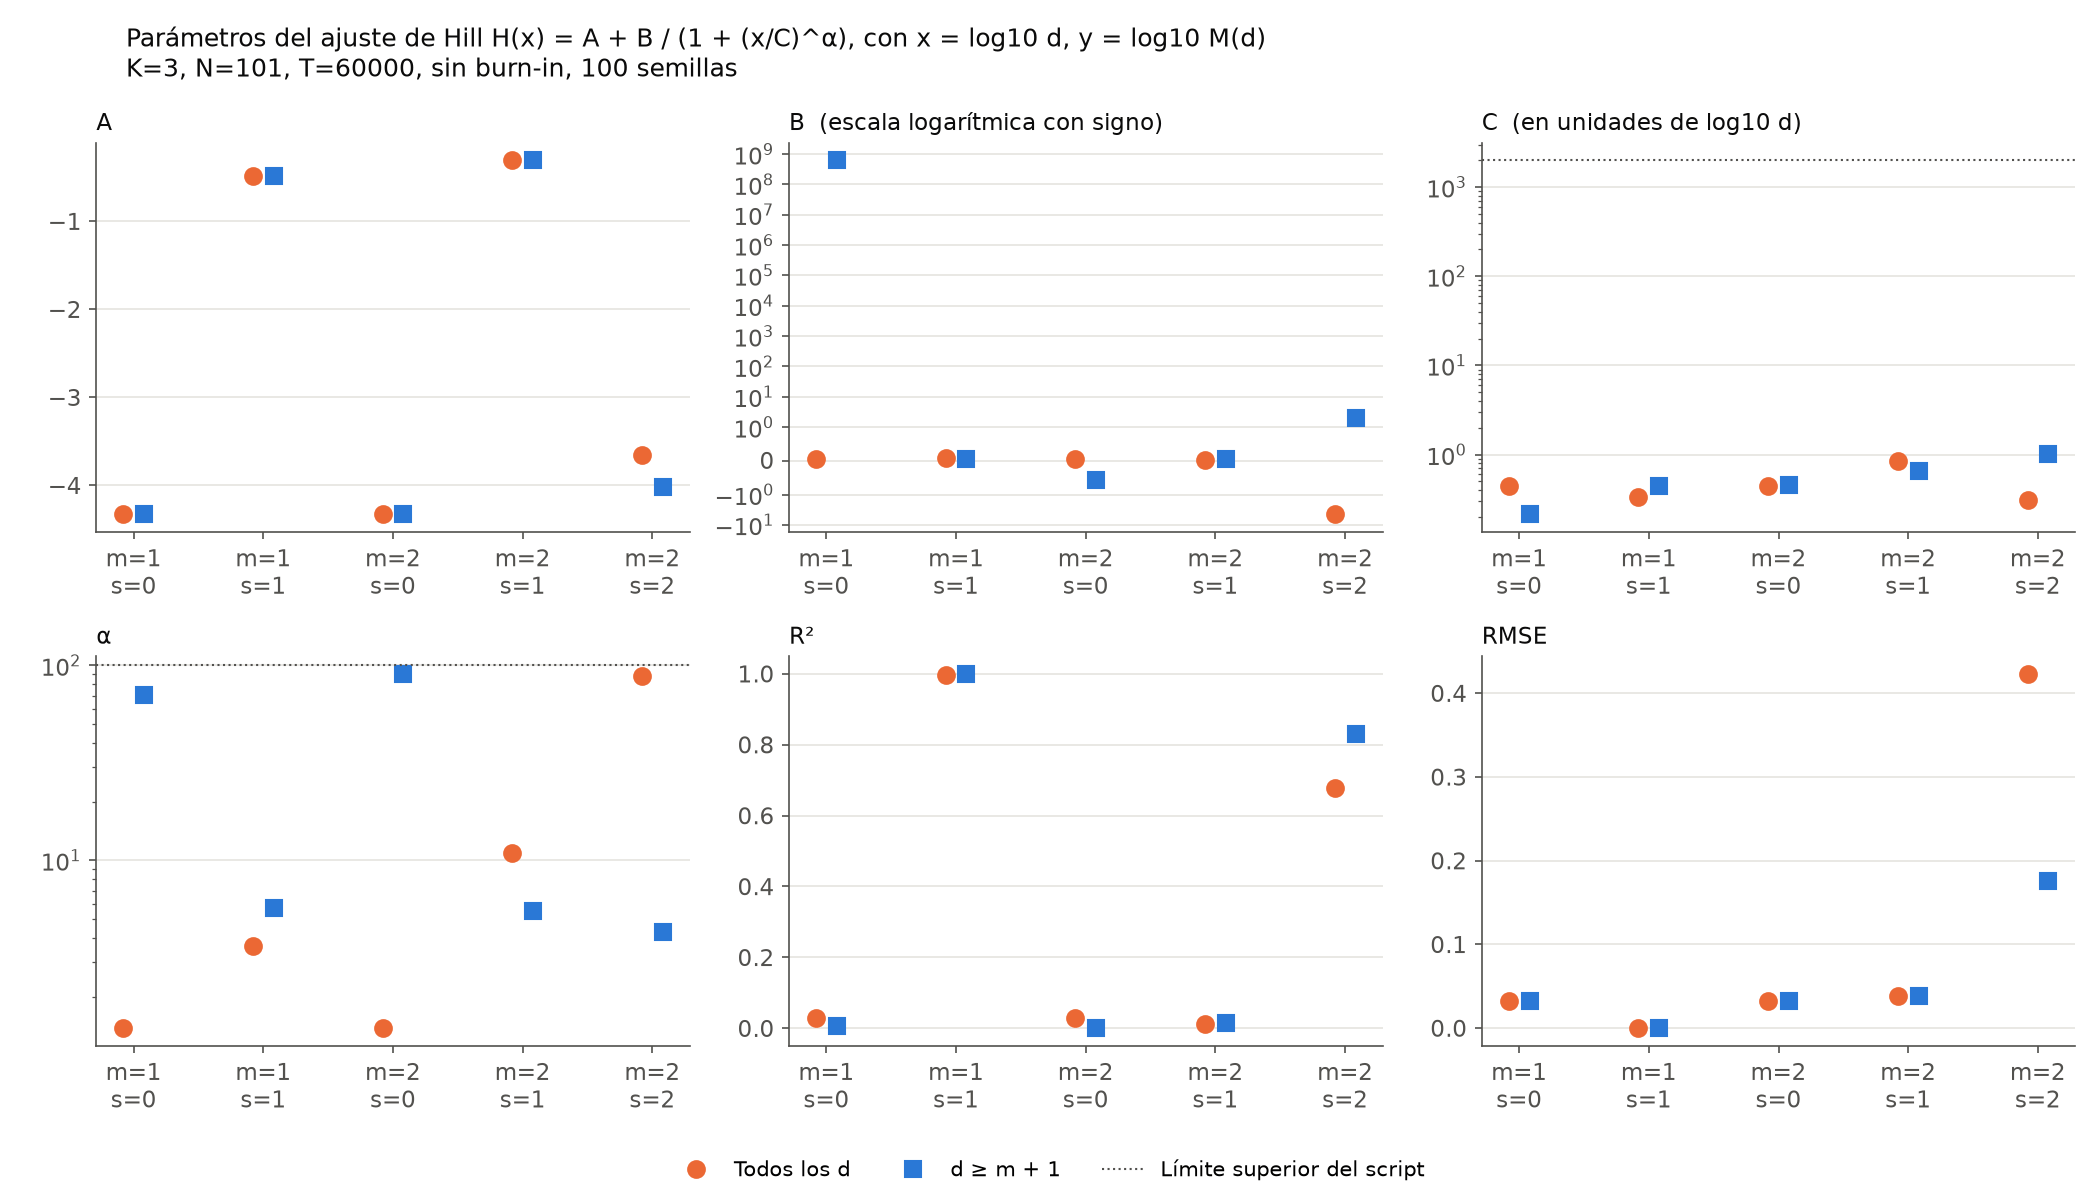
\includegraphics[width=0.92\textwidth]{figuras/Fase12_parametros_hill_N101_T60000.png}
\caption{Fase 12, parámetros de Hill de cada caso con los dos rangos de ajuste. $B$ en escala symlog y $C$, $\alpha$ en escala logarítmica; las líneas marcan los límites de búsqueda del script.}
\end{figure}
\begin{figure}[H]
\centering
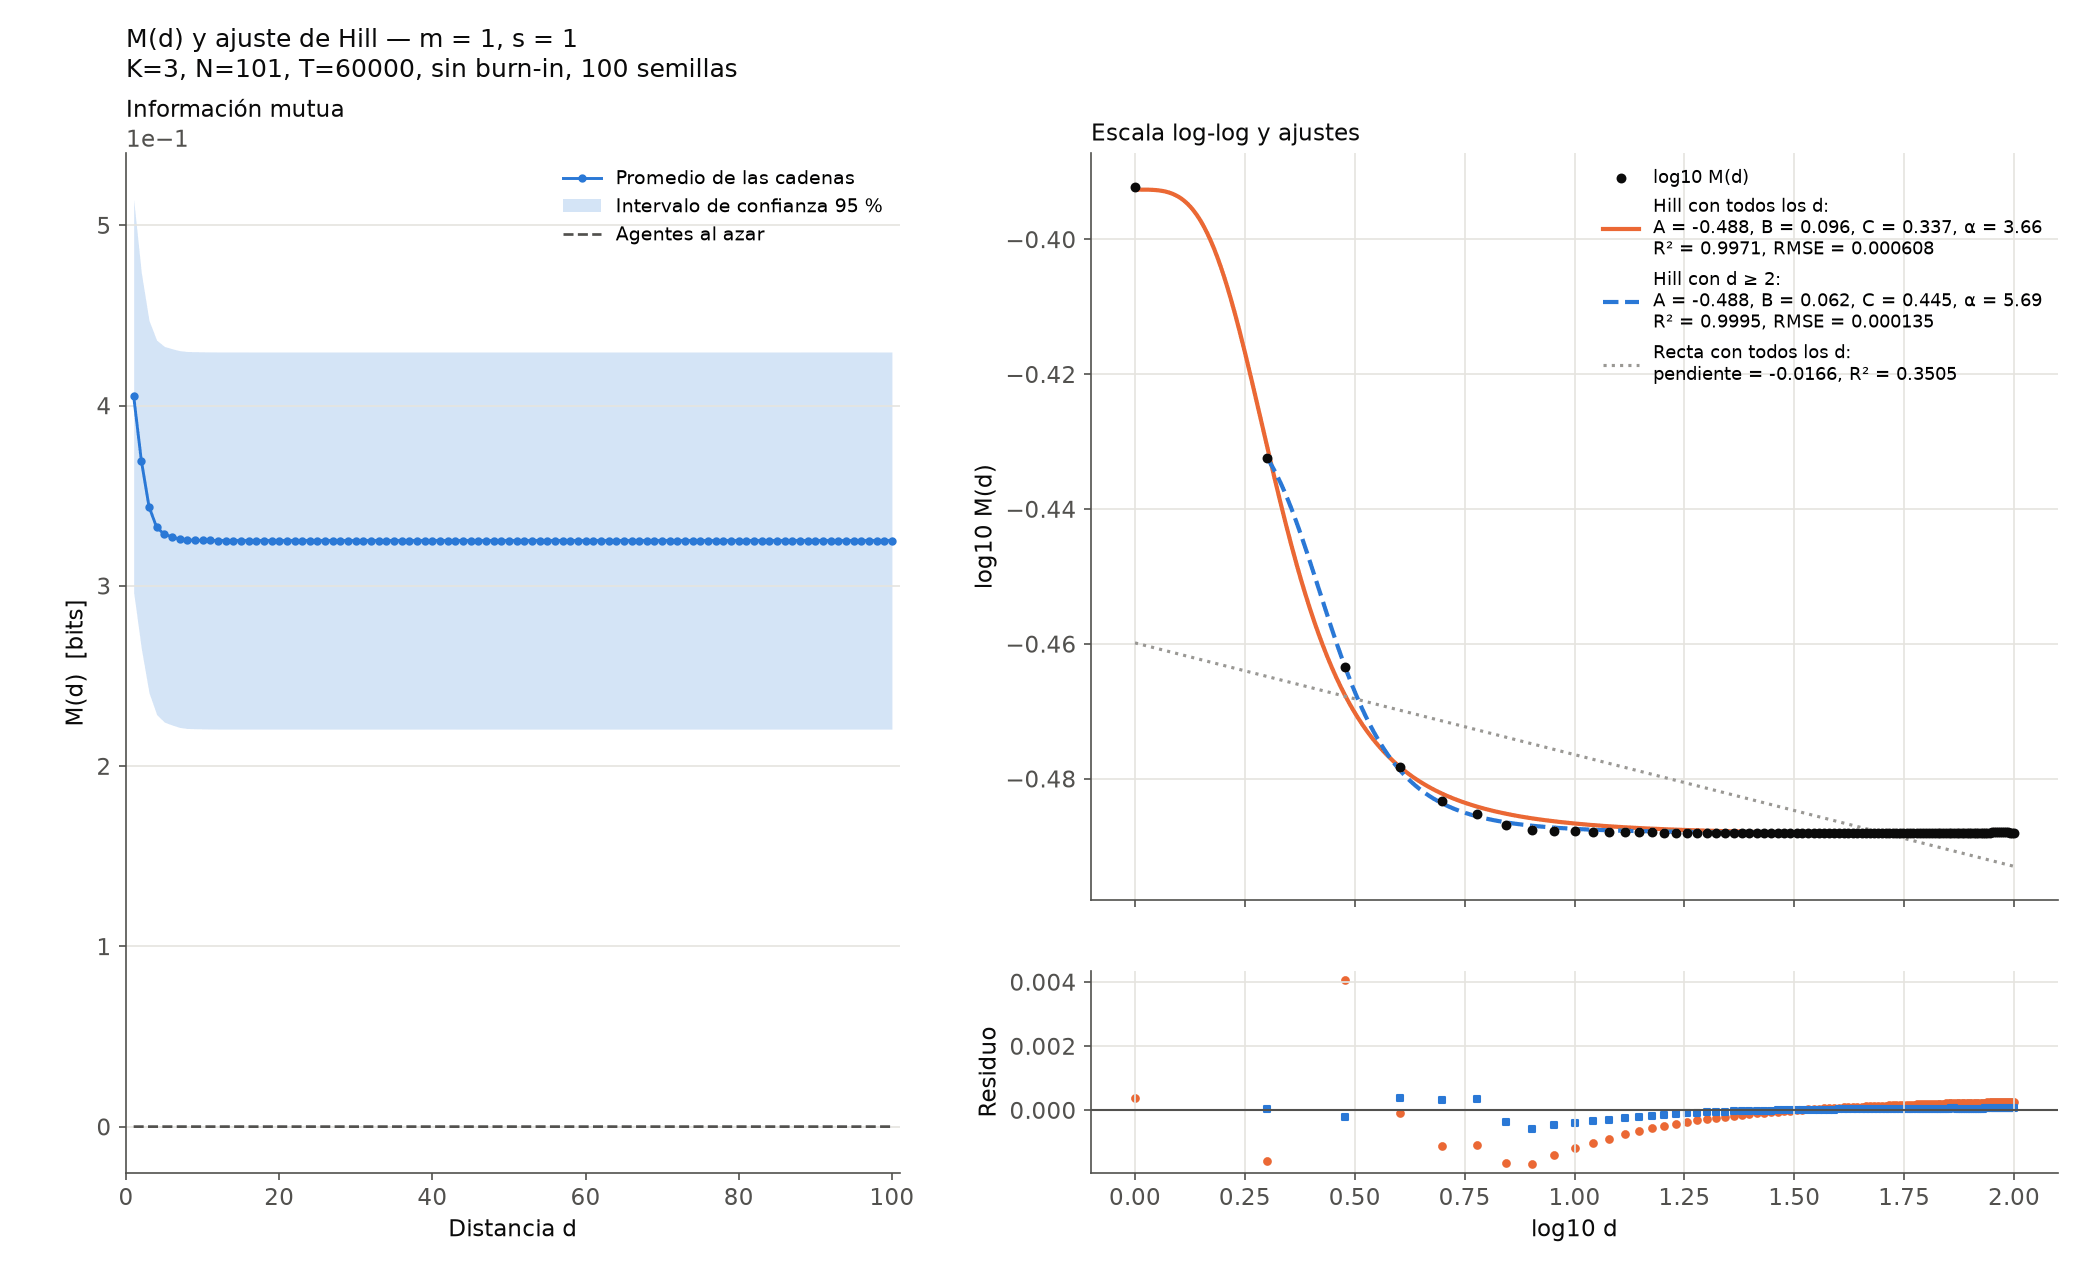
\includegraphics[width=0.92\textwidth]{figuras/Fase12_Md_hill_N101_m1_s1_T60000.png}
\caption{$m=1$, $s=1$: $M(d)$ (izquierda), log-log con los ajustes (derecha) y residuos.}
\end{figure}
\begin{figure}[H]
\centering
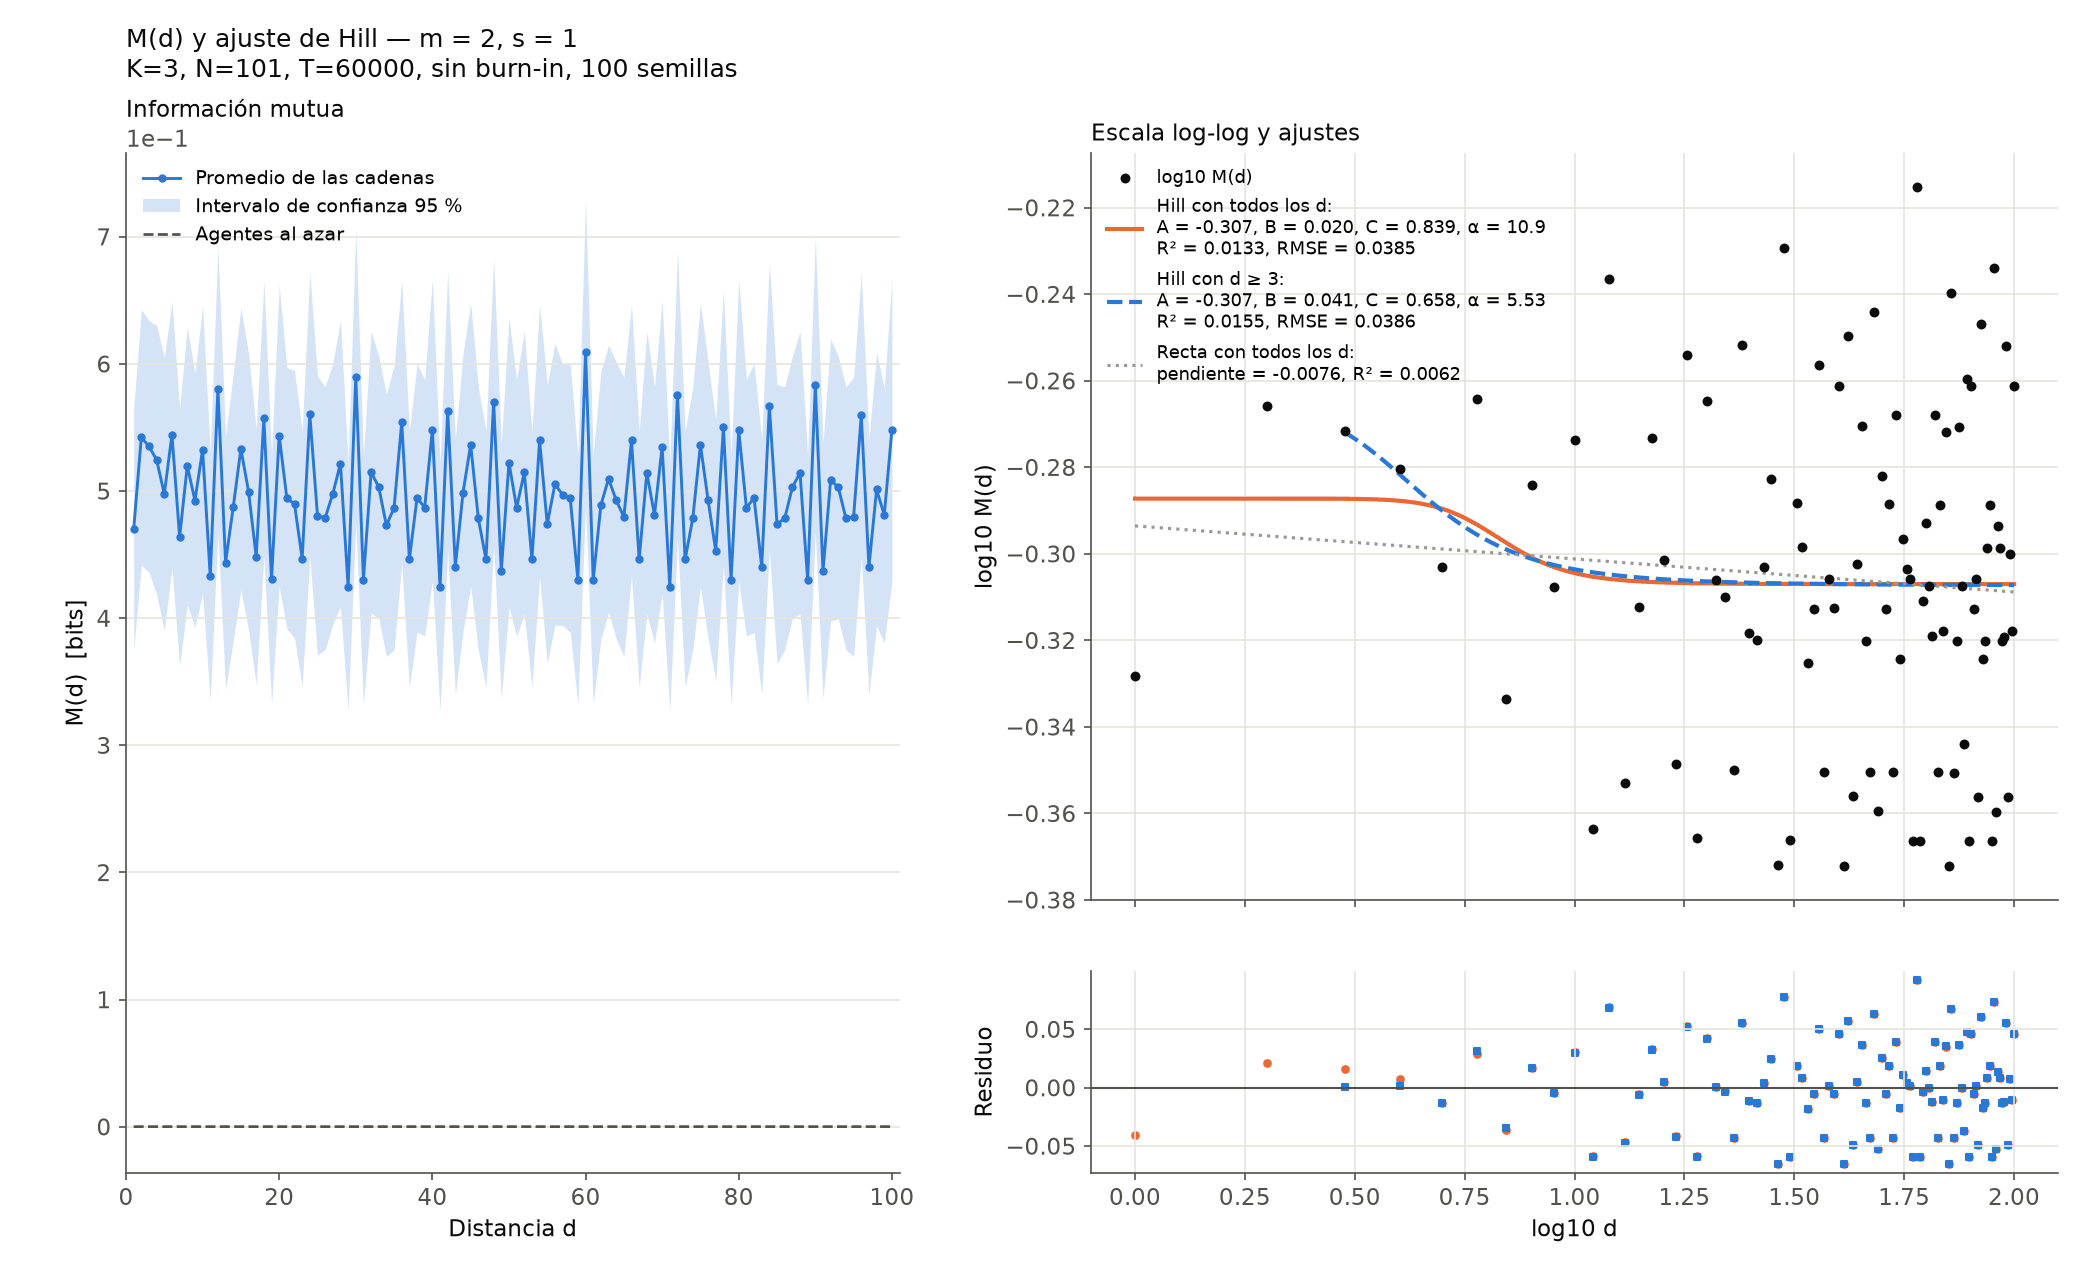
\includegraphics[width=0.92\textwidth]{figuras/Fase12_Md_hill_N101_m2_s1_T60000.png}
\caption{$m=2$, $s=1$.}
\end{figure}
\begin{figure}[H]
\centering
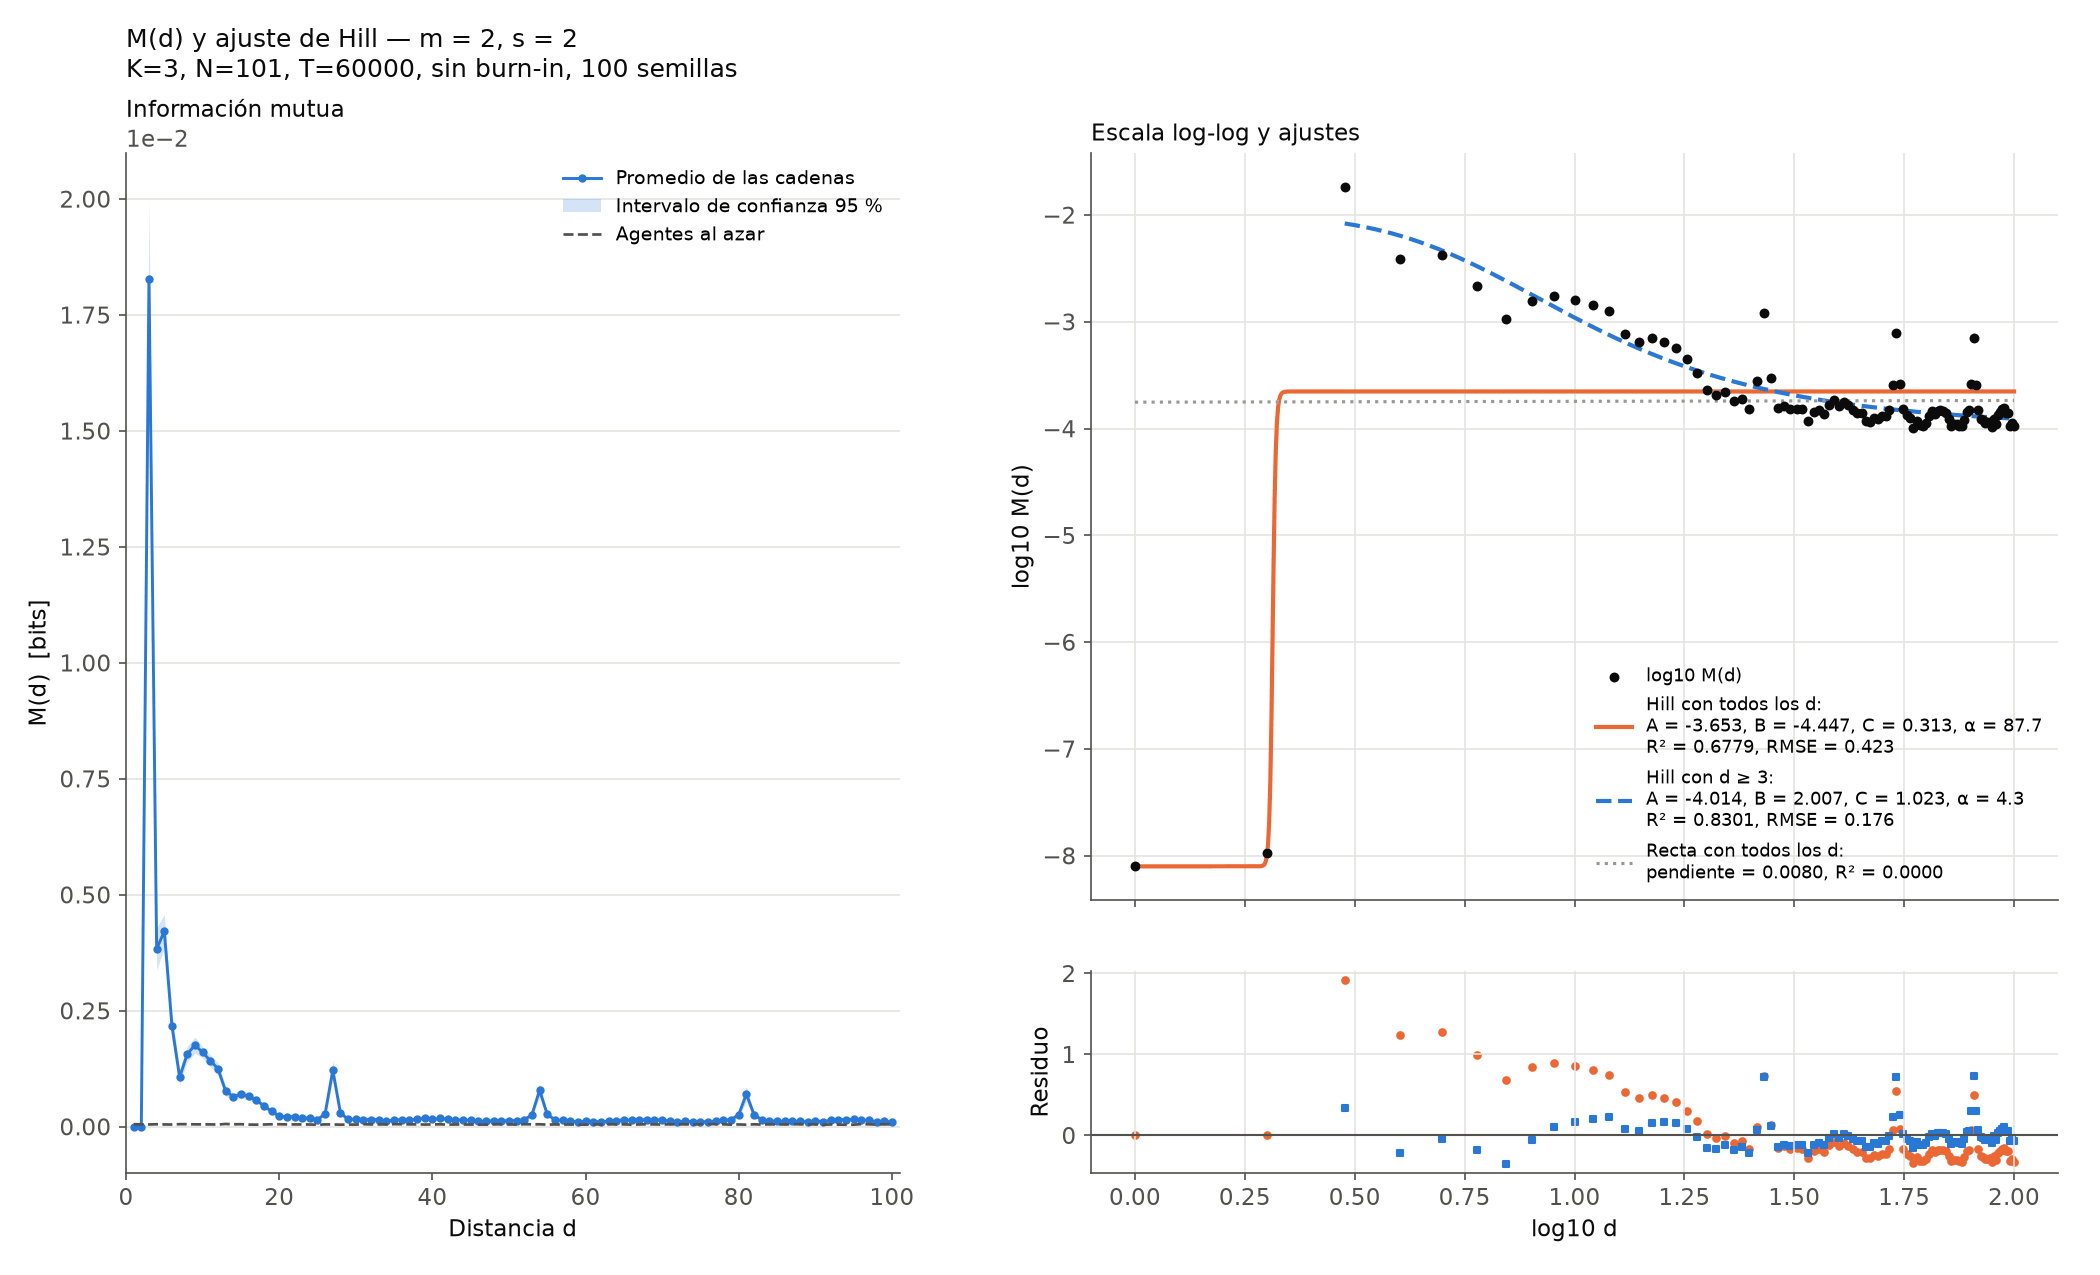
\includegraphics[width=0.92\textwidth]{figuras/Fase12_Md_hill_N101_m2_s2_T60000.png}
\caption{$m=2$, $s=2$.}
\end{figure}
\begin{figure}[H]
\centering
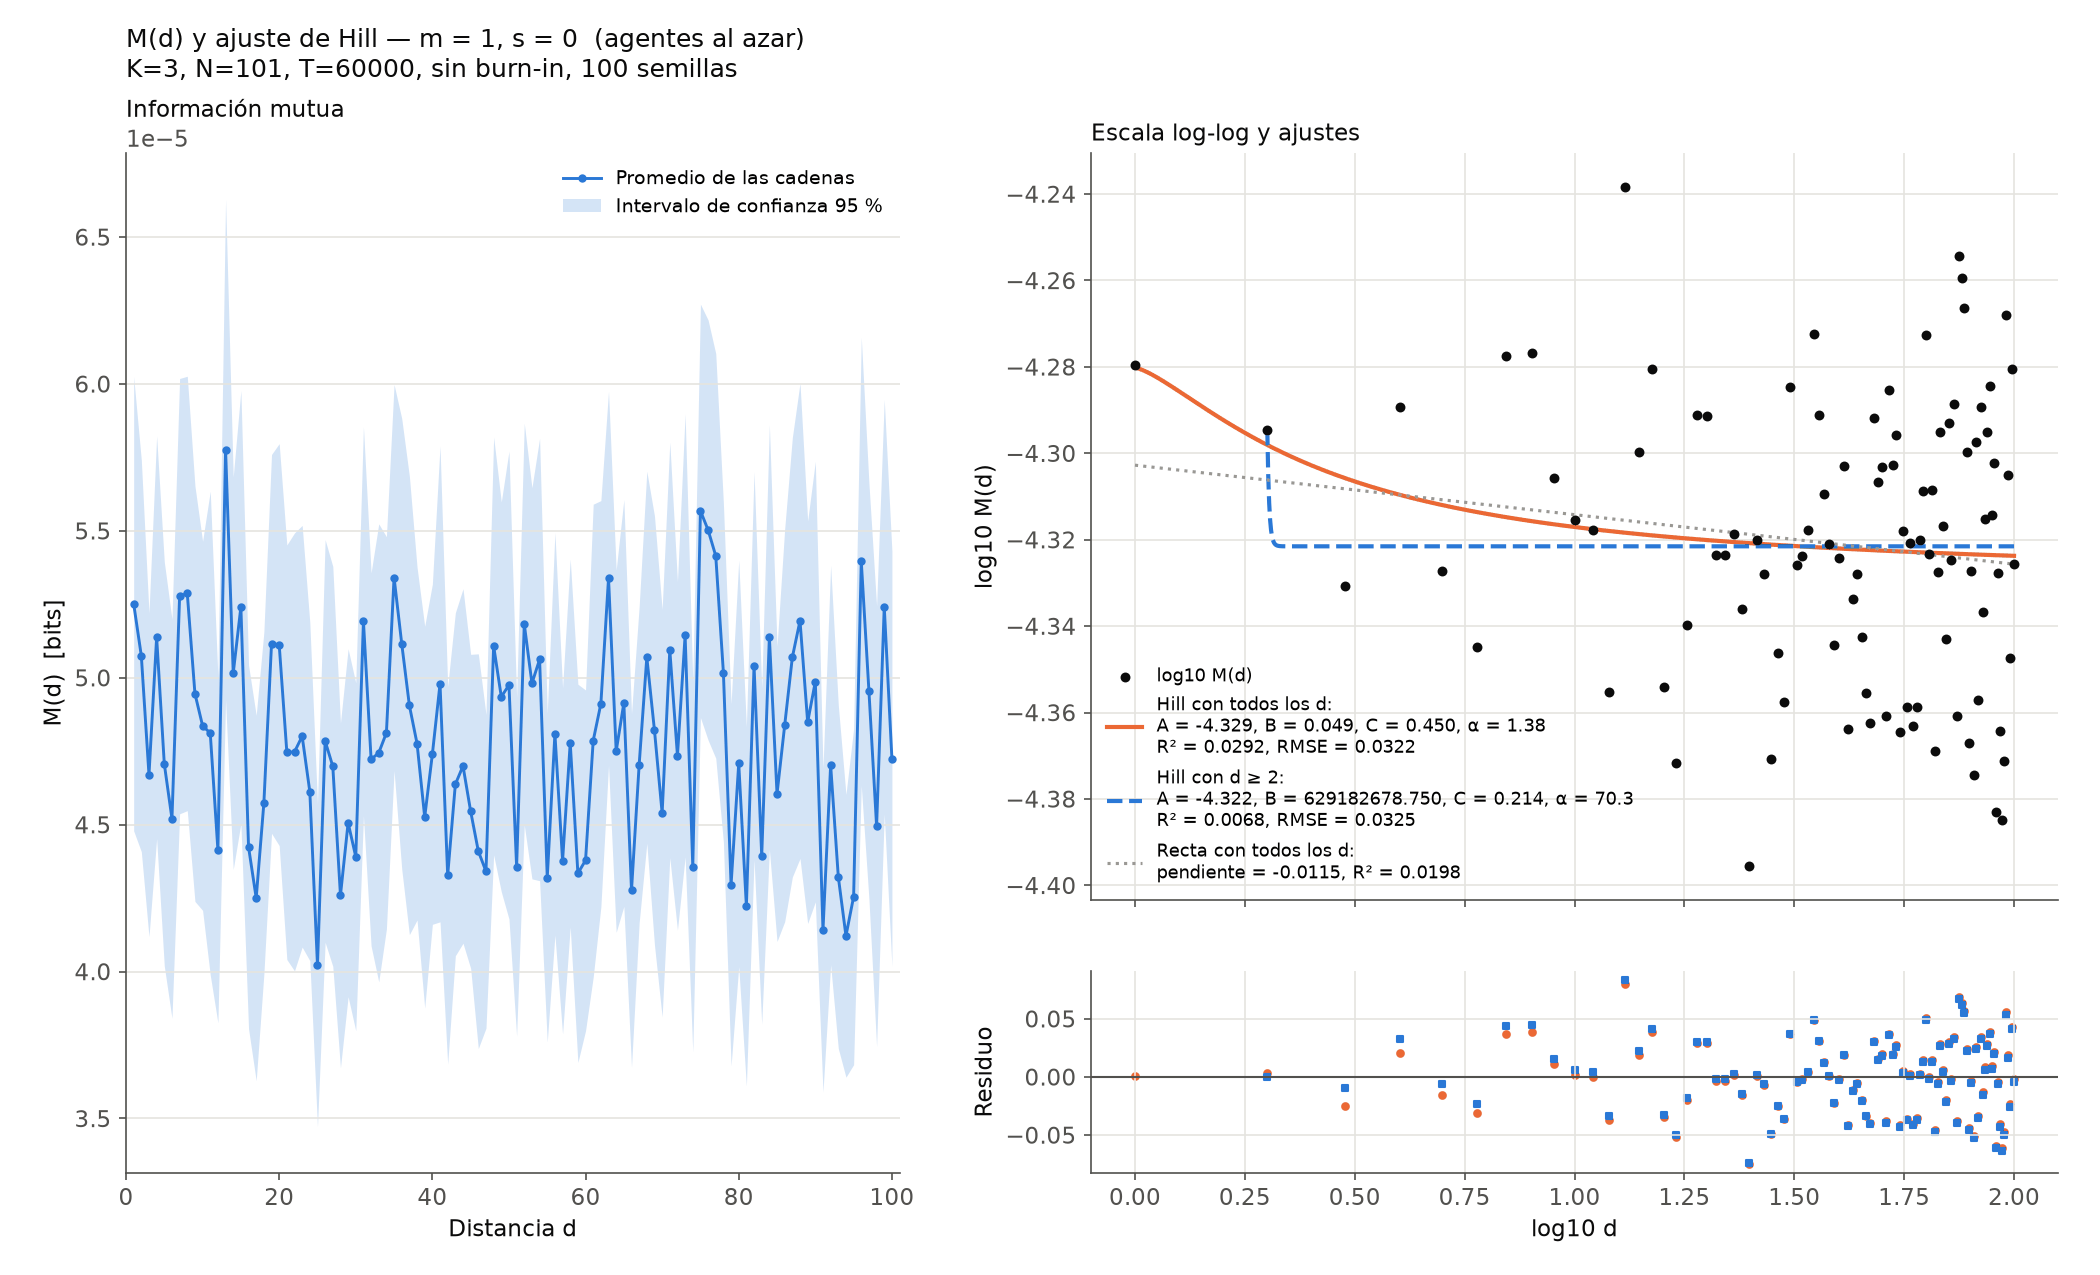
\includegraphics[width=0.92\textwidth]{figuras/Fase12_Md_hill_N101_m1_s0_T60000.png}
\caption{$m=1$, $s=0$ (agentes al azar).}
\end{figure}
\begin{figure}[H]
\centering
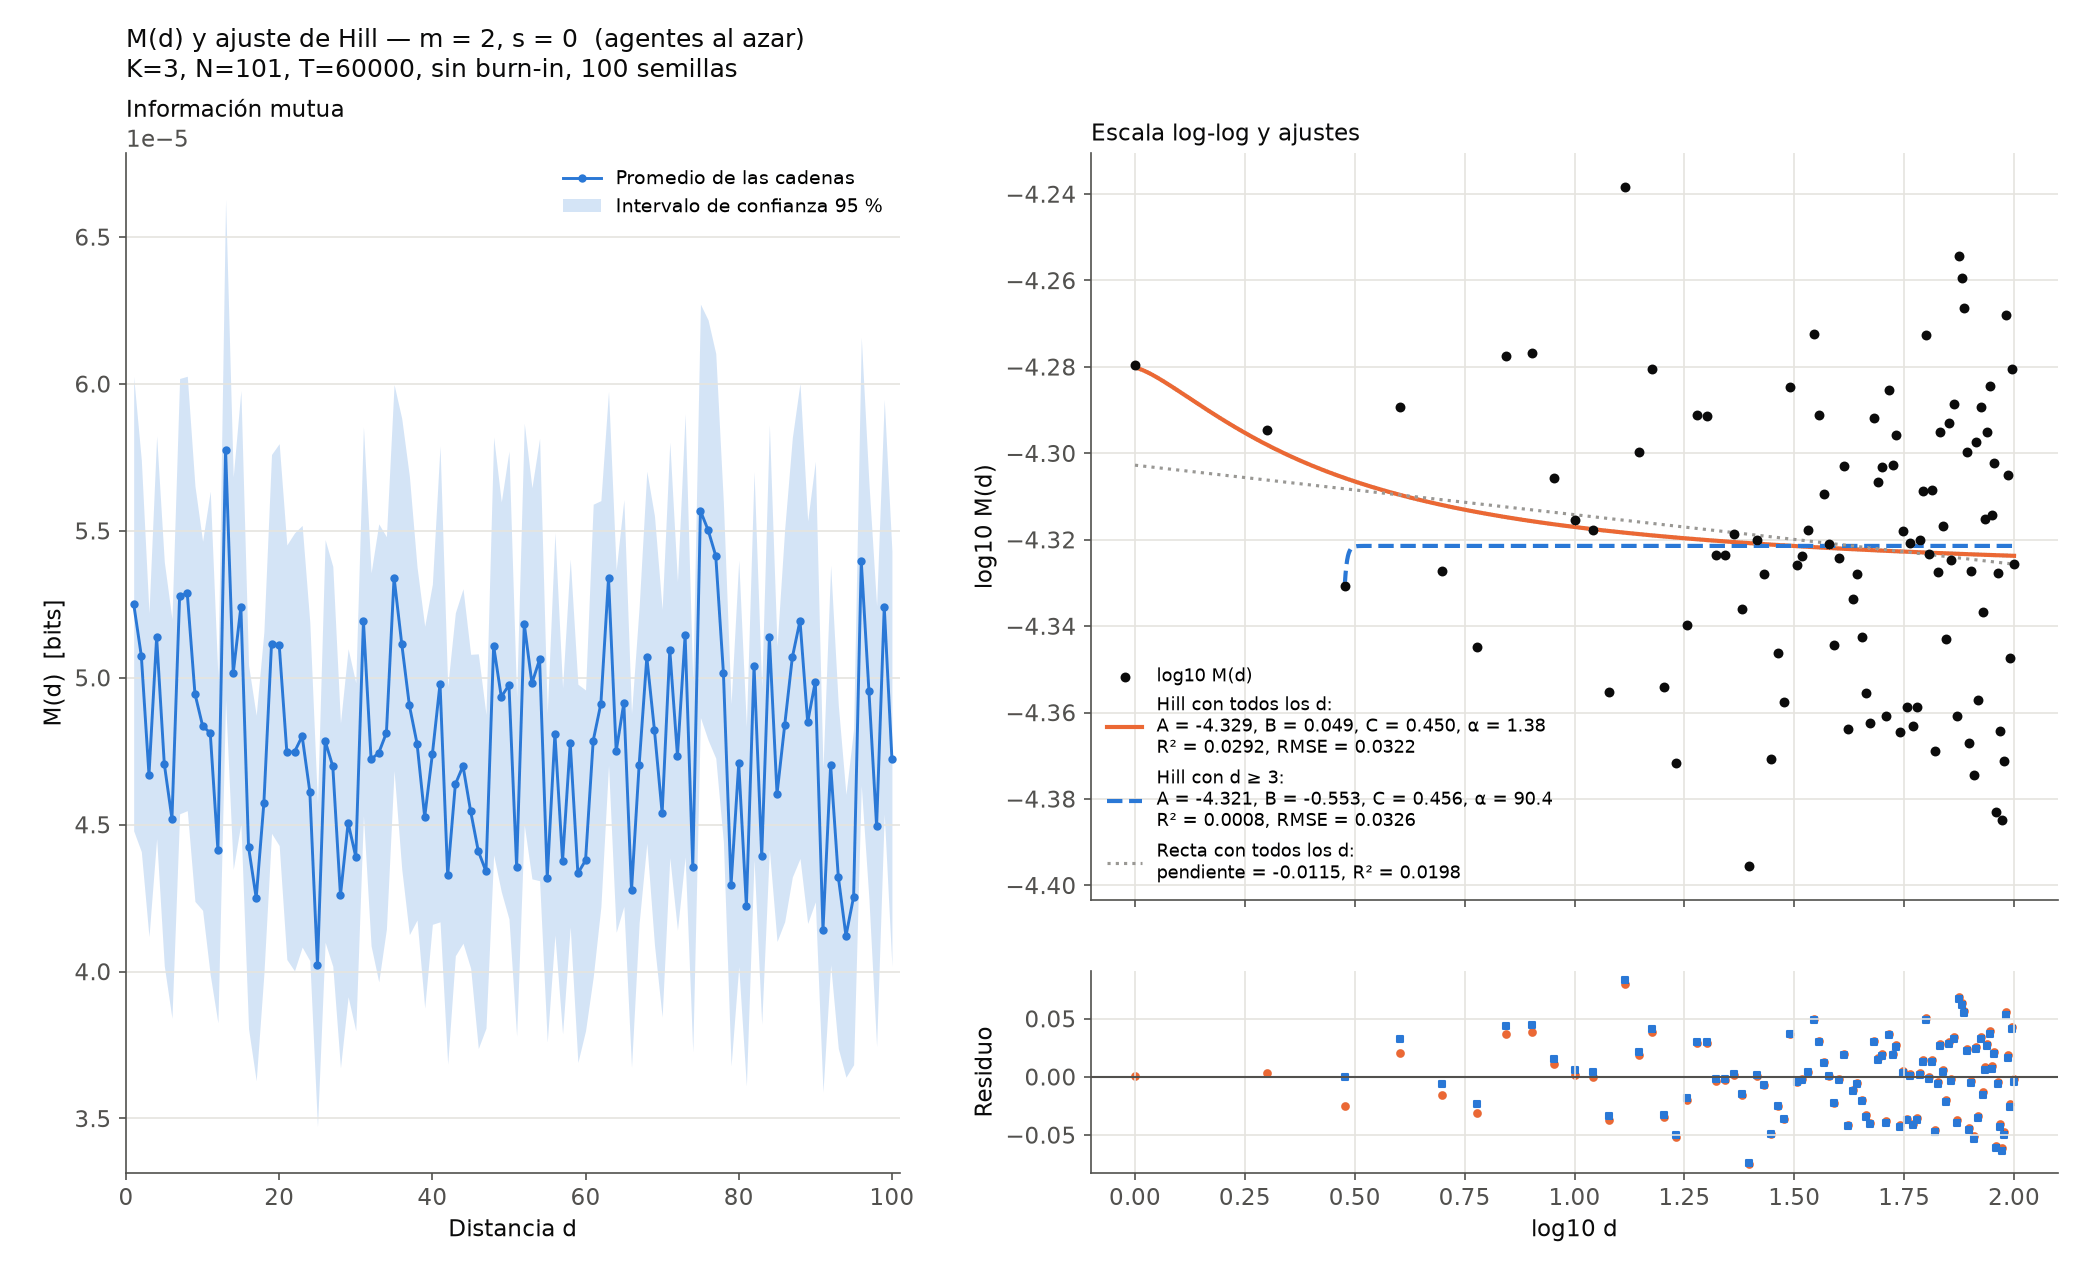
\includegraphics[width=0.92\textwidth]{figuras/Fase12_Md_hill_N101_m2_s0_T60000.png}
\caption{$m=2$, $s=0$ (agentes al azar; mismos datos que $m=1$, $s=0$, solo cambia el ajuste desde $d\ge 3$).}
\end{figure}

\subsubsection*{Observaciones}
\textbf{La función de Hill describe la forma solo en 2 de los 5 casos}, y en uno de ellos únicamente desde $d=3$.
\begin{itemize}
\item \textbf{$m=1$, $s=1$: sí} ($R^2=0.997$ y 0.9995). $M(d)$ baja y luego se queda plana, que es la forma de Hill. La caída es pequeña: de 0.41 a 0.33 bits. Al quitar $d=1$, $B$ baja de 0.096 a 0.062, $d_C$ pasa de 2.2 a 2.8 y $\alpha$ de 3.7 a 5.7.
\item \textbf{$m=2$, $s=2$: solo desde $d=3$} ($R^2=0.83$, sin avisos). Con todos los $d$ ($R^2=0.68$) el ajuste se dedica al salto entre $M(1),M(2)\approx10^{-8}$ y $M(3)\approx 2\times10^{-2}$: $\alpha$ sale 88, casi en el límite de 100, y el script avisa que los parámetros están mal determinados. Desde $d=3$, el ajuste baja de unos $10^{-2}$ a $10^{-4}$ bits, con $d_C\approx 10.5$ y $\alpha=4.3$; los picos en 27, 54 y 81 quedan como residuos.
\item \textbf{$s=0$ (agentes al azar): no} ($R^2=0.03$ o menos). La curva es plana, alrededor de $5\times10^{-5}$ bits, el valor esperado para una serie al azar con $T=60000$ ($4.8\times10^{-5}$). Los ajustes desde $d\ge m+1$ están degenerados: convergieron 3 y 2 de 30 arranques, $B$ llega a $6\times10^8$ y el script avisa que los parámetros están mal determinados.
\item \textbf{$m=2$, $s=1$: no} ($R^2\approx 0.01$). $M(d)$ es grande (0.47 a 0.61 bits) y oscila con $d$ sin decaer.
\item \textbf{Las cadenas con $s=1$ son muy distintas entre sí.} Con $m=1$, $M(100)$ es menor que $10^{-3}$ en 71 cadenas, está entre $10^{-3}$ y 1.5 en 23 y es mayor o igual que 1.5 (cerca del máximo, $\log_2 3=1.585$) en 6. Con $m=2$ los números son 47, 39 y 14. El promedio mezcla cadenas casi periódicas con otras casi al azar. No investigué más este punto.
\item \textbf{La recta log-log} tiene pendiente casi nula en los cinco casos ($-0.017$ a $+0.008$) y $R^2$ de 0.35 o menos.
\end{itemize}
En resumen, cuando $M(d)$ decae, Hill describe bien esa caída; cuando no decae (azar, o $m=2$, $s=1$), no hay forma que describir.

\section{Comprobaciones realizadas}
\begin{longtable}{p{7.6cm}p{7.6cm}}
\caption{Comprobaciones. Las de ``idéntico'' usan \texttt{np.array\_equal}.}\\
\toprule
Qué se comparó & Resultado\\
\midrule
\endfirsthead
\toprule
Qué se comparó & Resultado\\
\midrule
\endhead
\bottomrule
\endfoot
Fase 9: regla vieja, $N=50$, $m=3$, sin y con puntaje, contra \texttt{Ref Fase 2} & $M(d)$ de las 100 cadenas idéntico en los dos casos\\
Fase 9: regla nueva, turno por turno, 24 cadenas (incluidas $N=4$ y 5 para forzar opciones vacías) & Siempre gana la menos elegida entre las no vacías; marca de moneda correcta\\
Fase 9: fórmulas de los precios & Coinciden con conteos hechos a mano, incluidos los casos especiales de Mansilla\\
Fase 9: \texttt{joblib} contra un núcleo, 4 casos completos con $N=101$ & Conteos, ganadores y monedas idénticos\\
Fase 9: resumen de 400 cadenas & Recalculado desde los conteos, coincide, incluida la elección de las cadenas destacadas\\
Fase 9, complejidad: precios recalculados contra \texttt{resumen\_fase9.csv} & Coinciden en las 400 cadenas\\
Fase 9: codificación binaria & Dos ejemplos a mano dan la serie esperada; exceso y cociente dan la misma serie en todas las cadenas, con $N=101$ y $N=10000$\\
Fase 9: función de complejidad con una serie 0101\dots & $C(l)=l-1$, como debe\\
Fase 9, $N=10000$: el notebook nuevo con $N=101$ & Conteos idénticos a los ya guardados\\
Fase 9, $N=10000$: funciones de análisis & Valores conocidos con series de prueba: normal, Laplace, Pareto de exponente 3, AR(1), $M(d)$ periódica\\
Fase 9, $N=10000$: \texttt{joblib} contra un núcleo & 10 cadenas de los casos B y G idénticas\\
Fase 11: $N=101$ y $N=10000$ contra la fase 9 ($m=2$, $s=2$, con puntaje) & Ganadores y conteos idénticos\\
Fase 11: \texttt{joblib} contra un núcleo ($N=5000$, 4 cadenas) & Idéntico\\
Fase 11: los 9 archivos \texttt{.npz} & 100 cadenas de 6000 turnos, semillas correctas, conteos que suman $N$, ganador siempre la opción no vacía menos elegida\\
Fase 11: $M(d)$ del CSV, recalculado desde los \texttt{.npz} con una función escrita aparte & Diferencia relativa máxima $4\times10^{-9}$ (redondeo del CSV)\\
Fase 11: re-ejecución tras corregir el título de la gráfica de resumen & Los dos CSV idénticos a los anteriores\\
Fase 12: agentes al azar contra la fase 8 & $M(d)$ de las 100 cadenas idéntico\\
Fase 12: $m=2$, $s=2$ contra la fase 7 & $M(d)$ de las 100 cadenas idéntico\\
\end{longtable}

\textbf{Lo que no se comprobó:}
\begin{itemize}
\item Que un núcleo dé lo mismo que varios con los $N$ grandes de la fase 11; solo se probó con $N=5000$.
\item Los picos de los espectros no se compararon con series de referencia, porque no se incluyeron referencias.
\item El valor teórico $C(2)\approx 0.082$ de la serie binaria de Mansilla no se comprobó con una corrida.
\item Las ráfagas de unos 730 turnos del caso F se vieron a ojo; no se midieron.
\item De las gráficas por caso de la fase 9 revisé a ojo todas las de precios, y las de series, hechos estilizados y medidas informacionales del caso A y la de series del caso F. Las otras 17 gráficas de $N=10000$ (series, hechos estilizados y medidas de B a G) están en el apéndice pero no las revisé una por una. Las de las fases 11 y 12 sí las revisé todas.
\item La fase 11 no se repitió con $T$ más largo ni con burn-in.
\end{itemize}

\section{Limitaciones y pendientes}
\begin{itemize}
\item \textbf{Regla nueva sin confirmar.} Falta confirmar con el Dr. Mansilla qué pasa cuando todos eligen la misma opción. Como nunca hubo opciones vacías, no afecta ningún resultado de este reporte. \texttt{reglas\_del\_modelo.md} y \texttt{CLAUDE.md} todavía describen solo la regla vieja.
\item \textbf{Comparación con el artículo de Mansilla}: aproximada, por la diferencia en la longitud de las series y porque no se sabe qué $l$ usó en su ajuste.
\item \textbf{Fase 11}: todos los valores de $N$ con $m=2$ quedaron en la misma zona; queda por discutir con el Dr. Mansilla si la periodicidad de 27 es propia de esa zona.
\item \textbf{Fase 12}: no se investigó por qué las cadenas con $s=1$ son tan distintas entre sí.
\item \textbf{Pendientes por decisión tuya:} comparación con índices reales (NASDAQ e IPC), burbujas con LPPL (apartado 6.8) y la validación del juego binario de la fase 8.
\end{itemize}

\appendix

\section{Fase 9, $N=101$: gráficas de precios}\label{ap:f9n101}
En cada figura, ``conjunto'' muestra las 100 cadenas en gris y la destacada en color; ``detalle'' muestra solo la destacada, con un acercamiento de 200 turnos del precio de Mansilla.
\subsection*{Caso A: $m=2$, sin puntaje}
\begin{figure}[H]
\centering
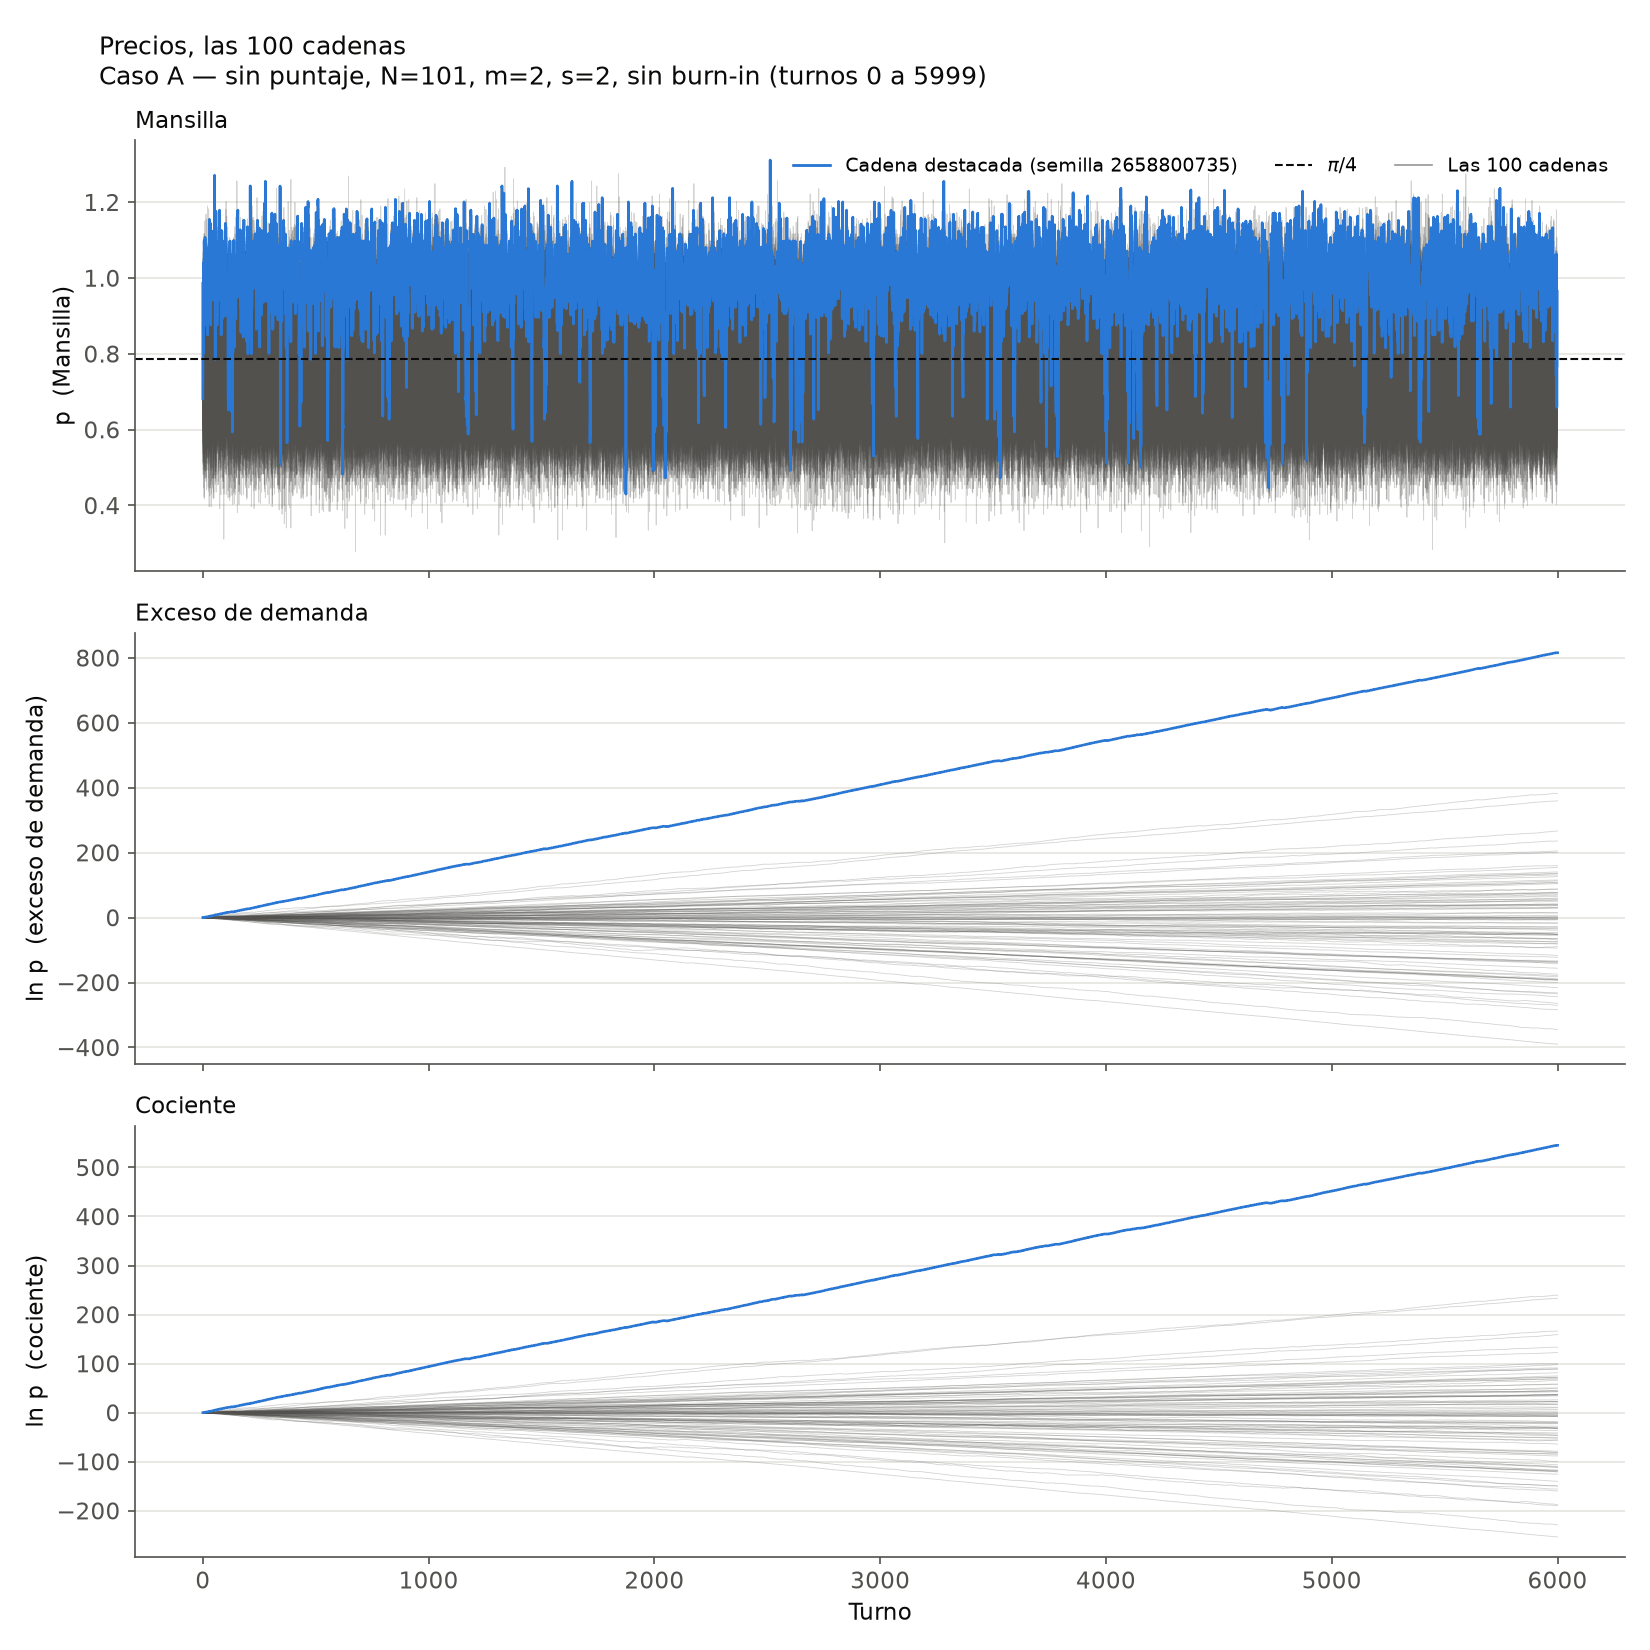
\includegraphics[width=0.49\textwidth]{figuras/Fase9_precios_conjunto_casoA_N101_m2_s2_sin_puntaje_T6000_regla_nueva_sin_burnin.png}\hfill
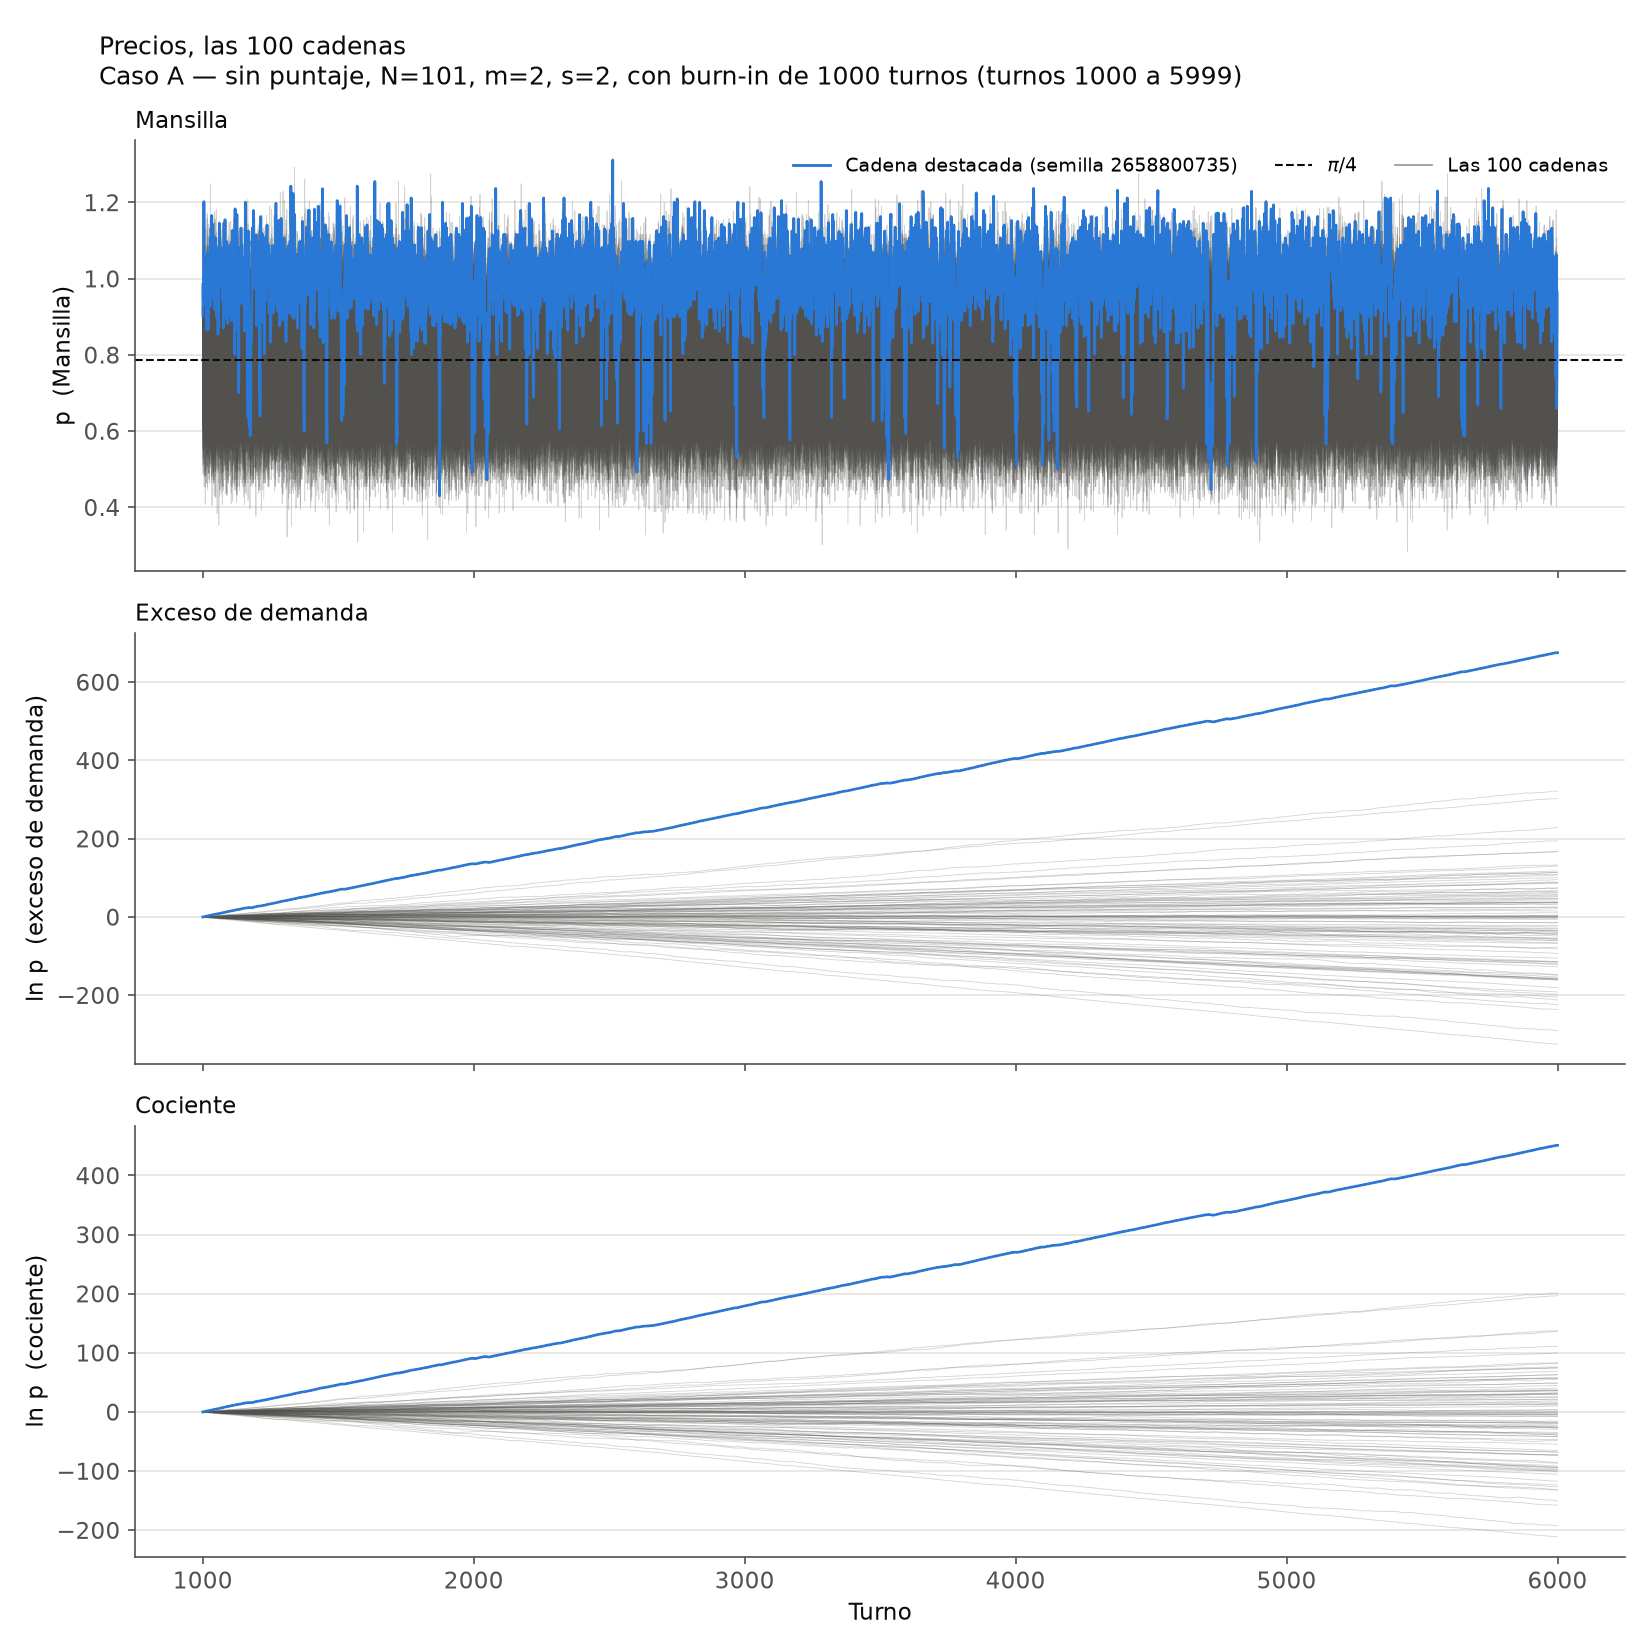
\includegraphics[width=0.49\textwidth]{figuras/Fase9_precios_conjunto_casoA_N101_m2_s2_sin_puntaje_T6000_regla_nueva_con_burnin1000.png}
\caption{Caso A, $N=101$: conjunto de precios sin burn-in (izquierda) y con burn-in de 1000 turnos (derecha).}
\end{figure}

\begin{figure}[H]
\centering
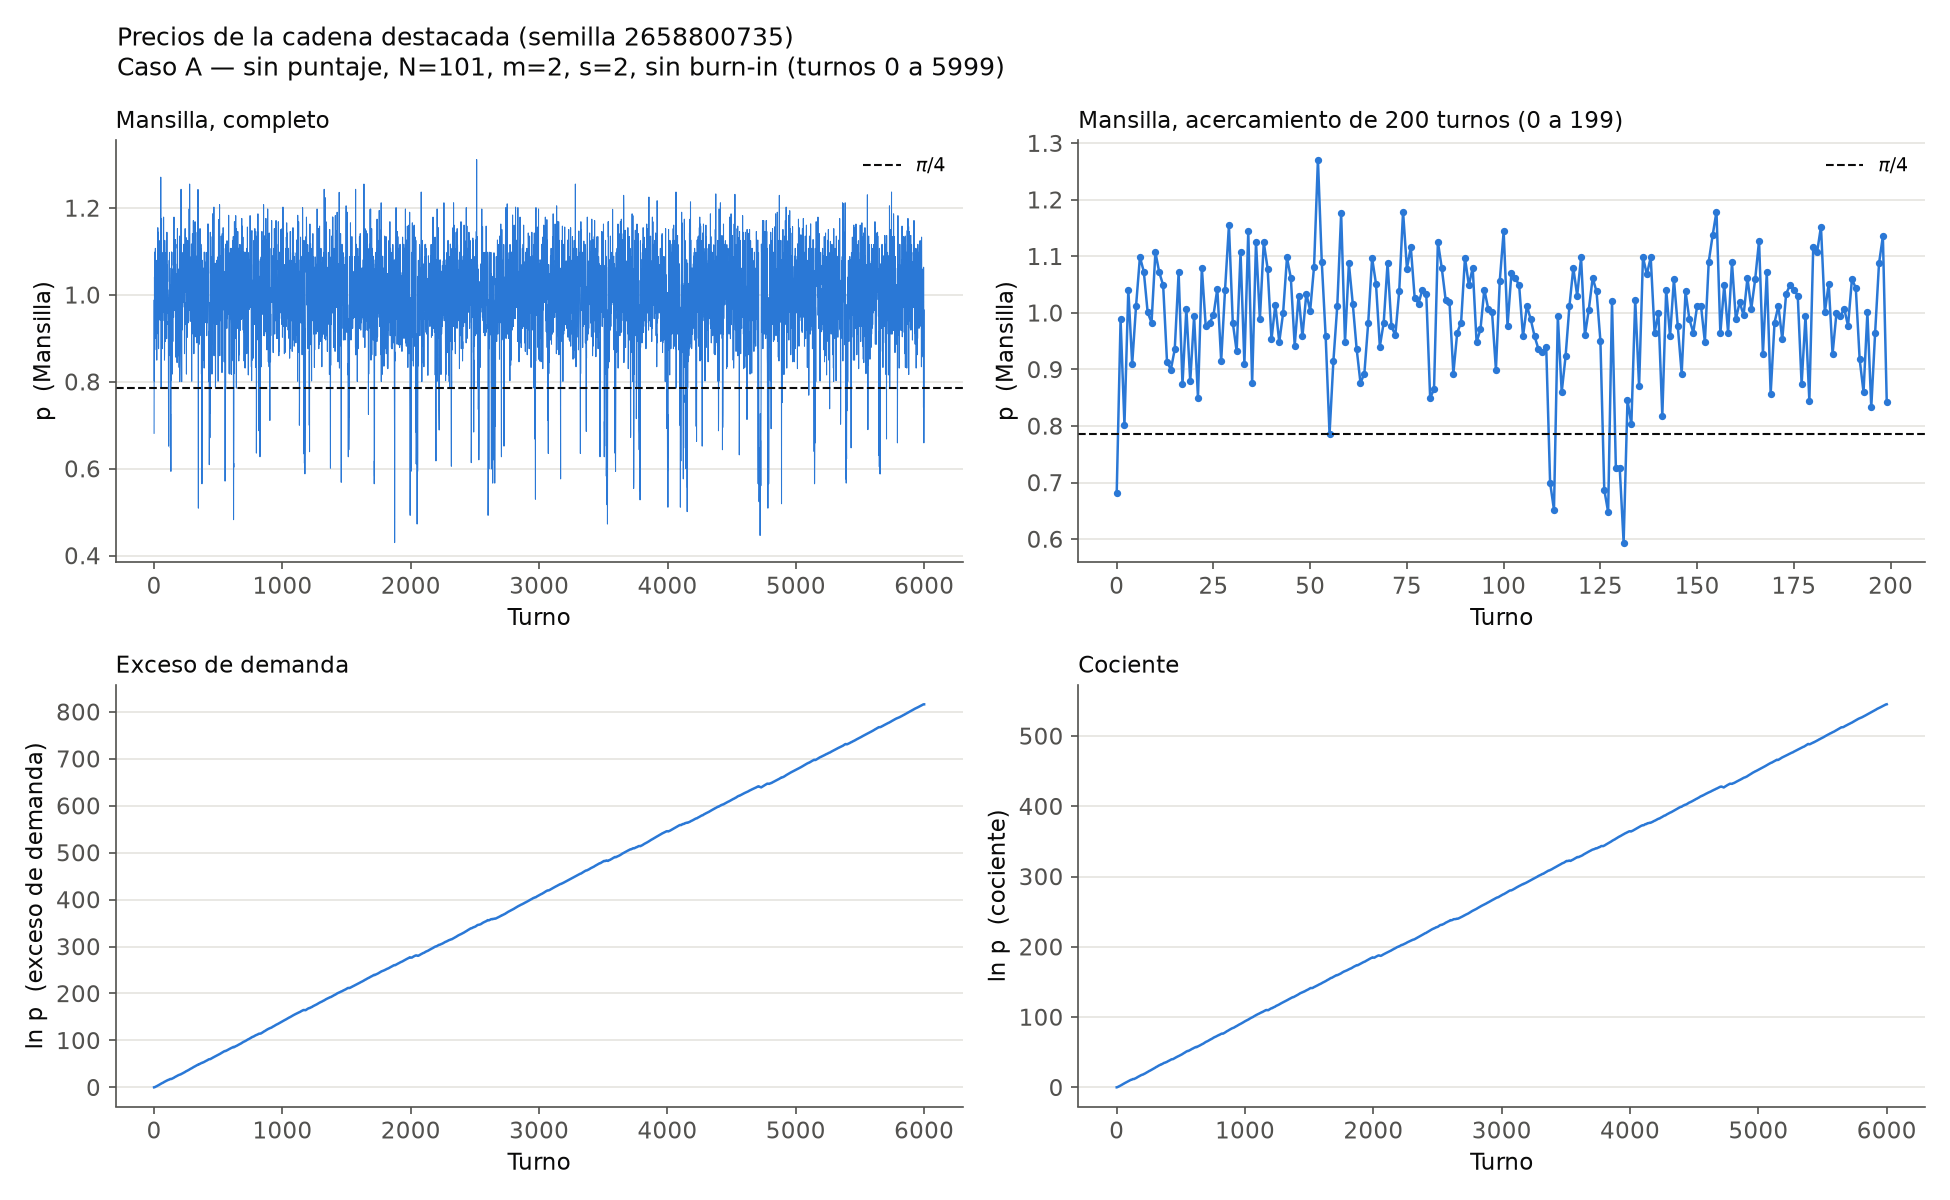
\includegraphics[width=0.49\textwidth]{figuras/Fase9_precios_detalle_casoA_N101_m2_s2_sin_puntaje_T6000_regla_nueva_sin_burnin.png}\hfill
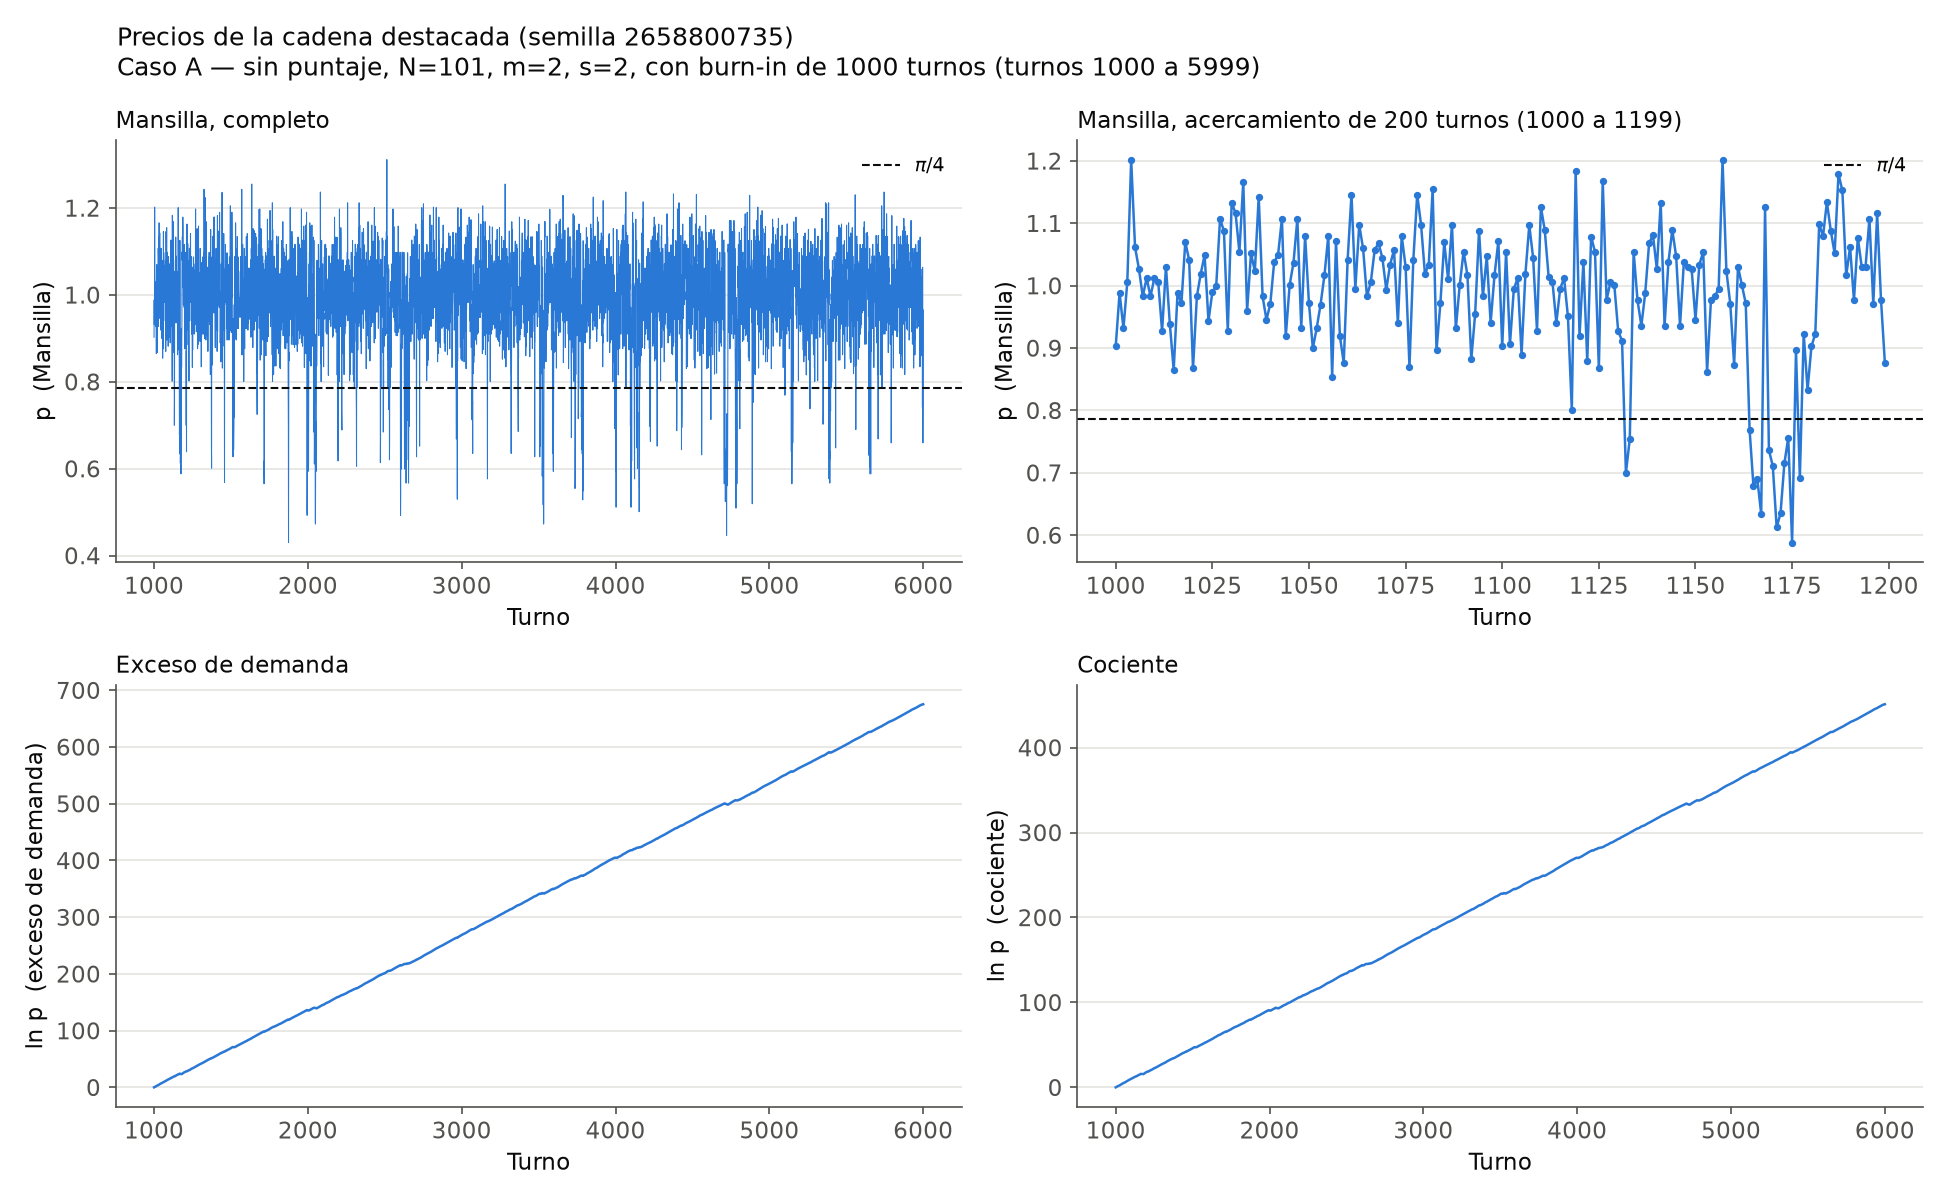
\includegraphics[width=0.49\textwidth]{figuras/Fase9_precios_detalle_casoA_N101_m2_s2_sin_puntaje_T6000_regla_nueva_con_burnin1000.png}
\caption{Caso A, $N=101$: detalle de la cadena destacada sin burn-in (izquierda) y con burn-in (derecha).}
\end{figure}

\subsection*{Caso B: $m=2$, con puntaje}
\begin{figure}[H]
\centering
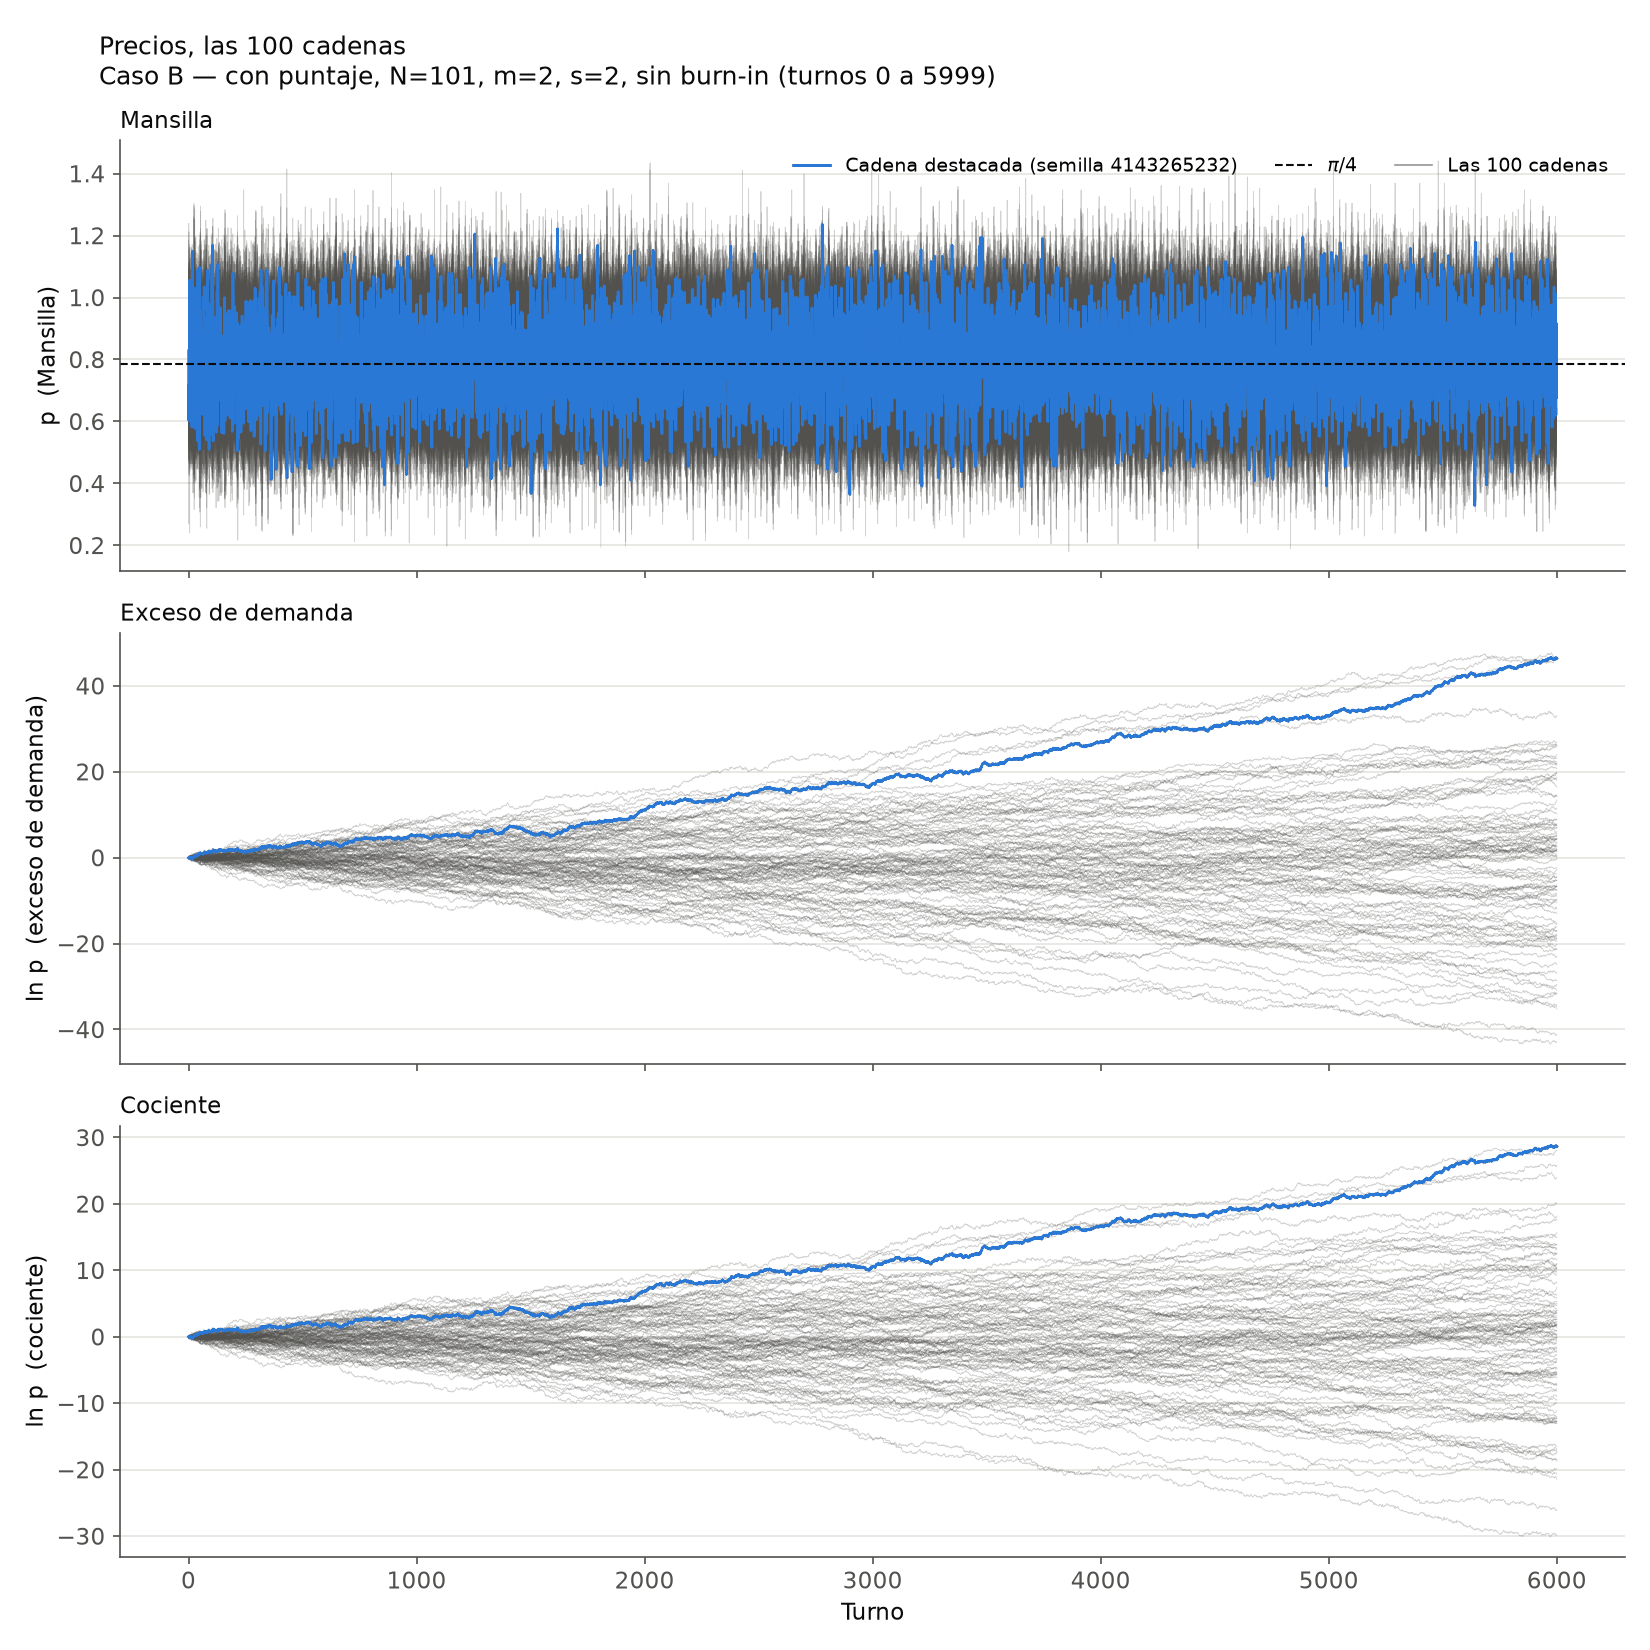
\includegraphics[width=0.49\textwidth]{figuras/Fase9_precios_conjunto_casoB_N101_m2_s2_con_puntaje_T6000_regla_nueva_sin_burnin.png}\hfill
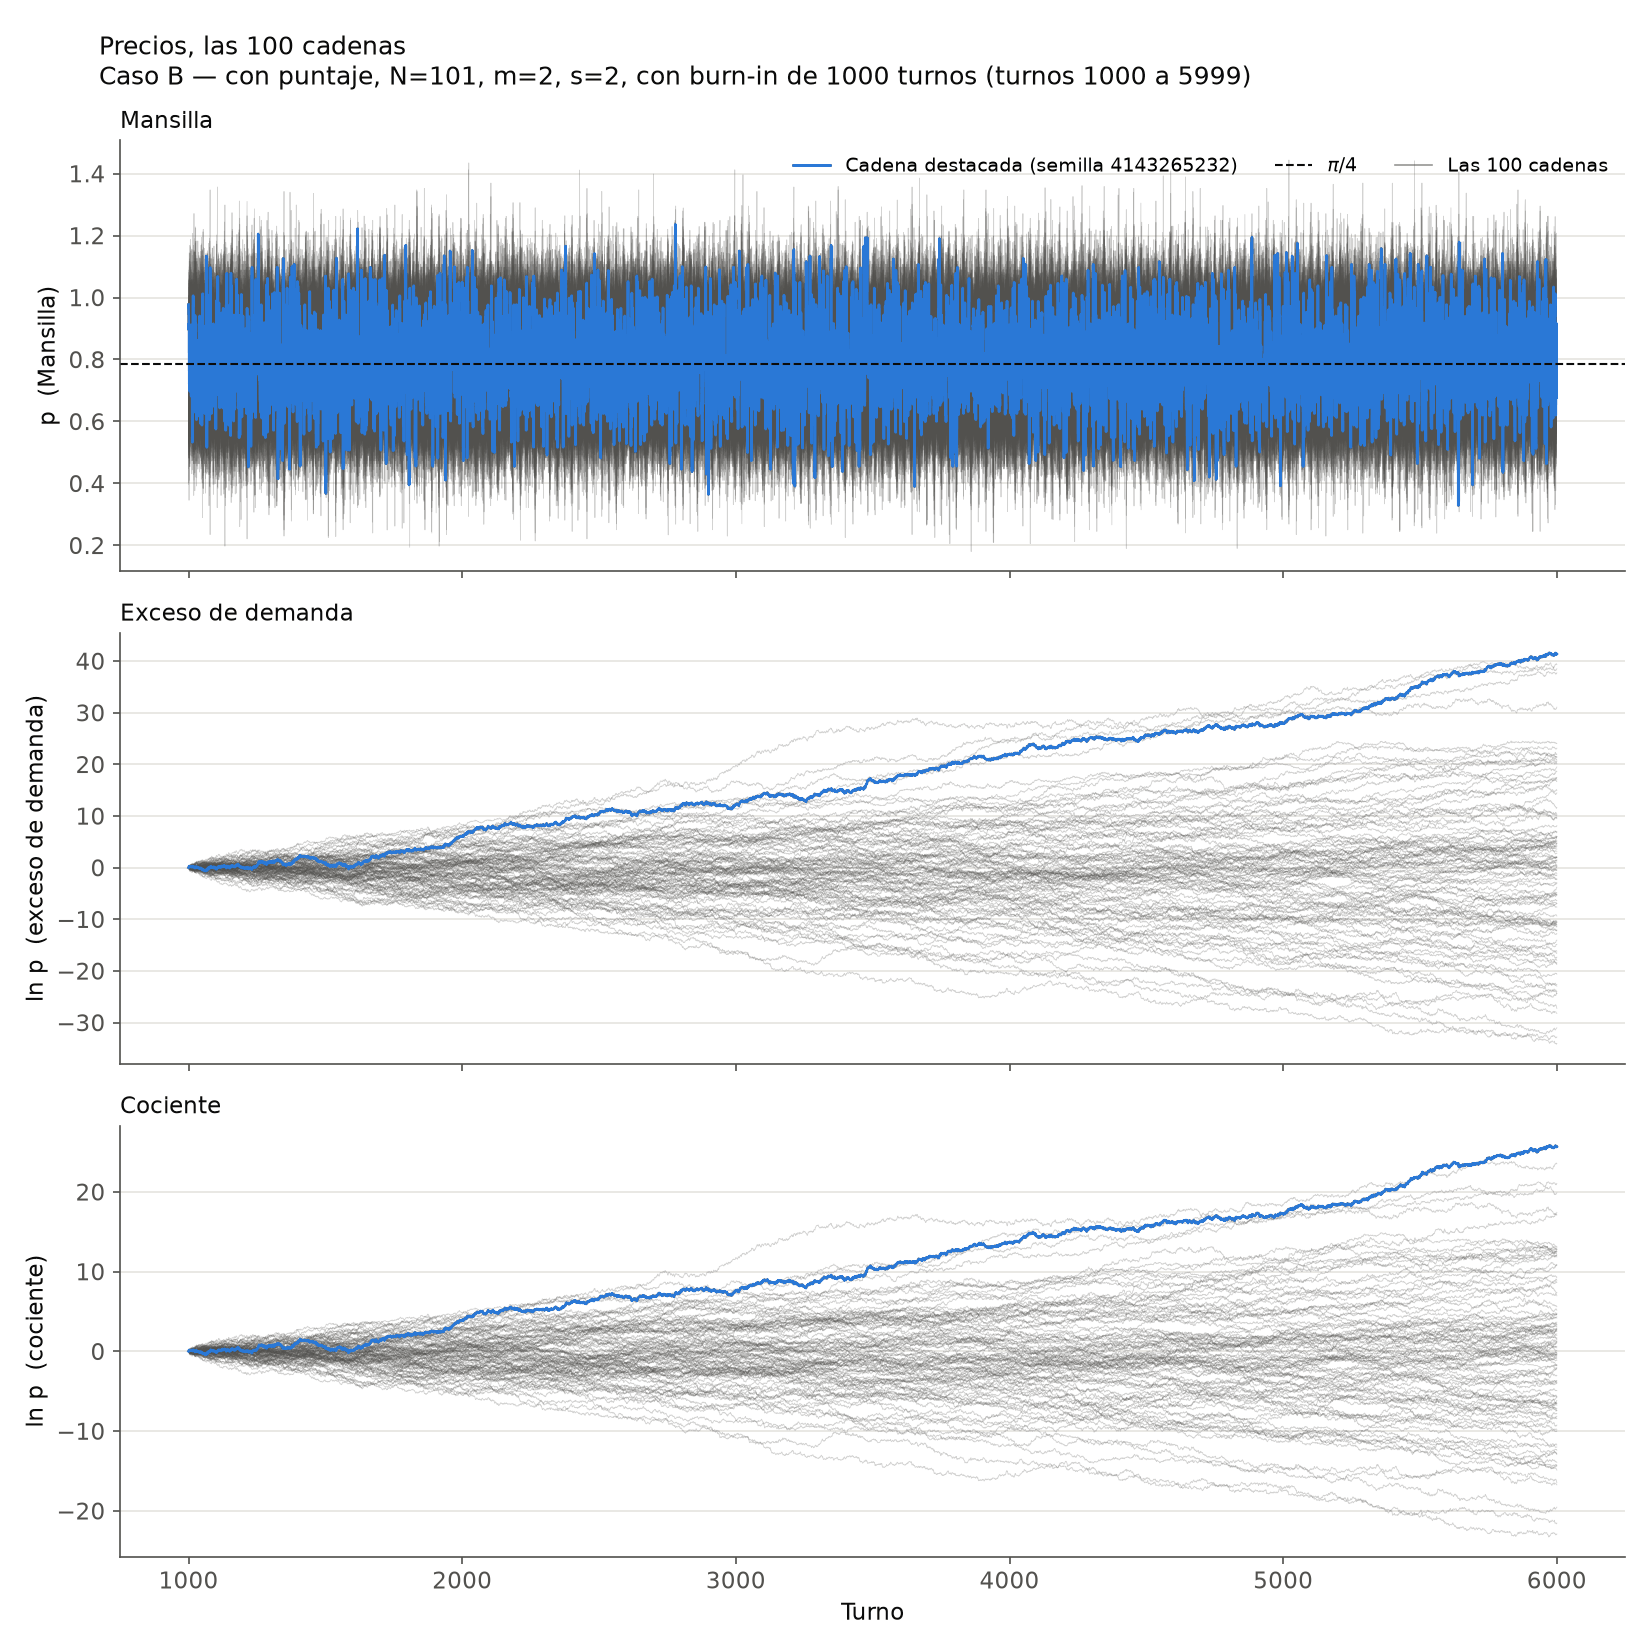
\includegraphics[width=0.49\textwidth]{figuras/Fase9_precios_conjunto_casoB_N101_m2_s2_con_puntaje_T6000_regla_nueva_con_burnin1000.png}
\caption{Caso B, $N=101$: conjunto de precios sin burn-in (izquierda) y con burn-in de 1000 turnos (derecha).}
\end{figure}

\begin{figure}[H]
\centering
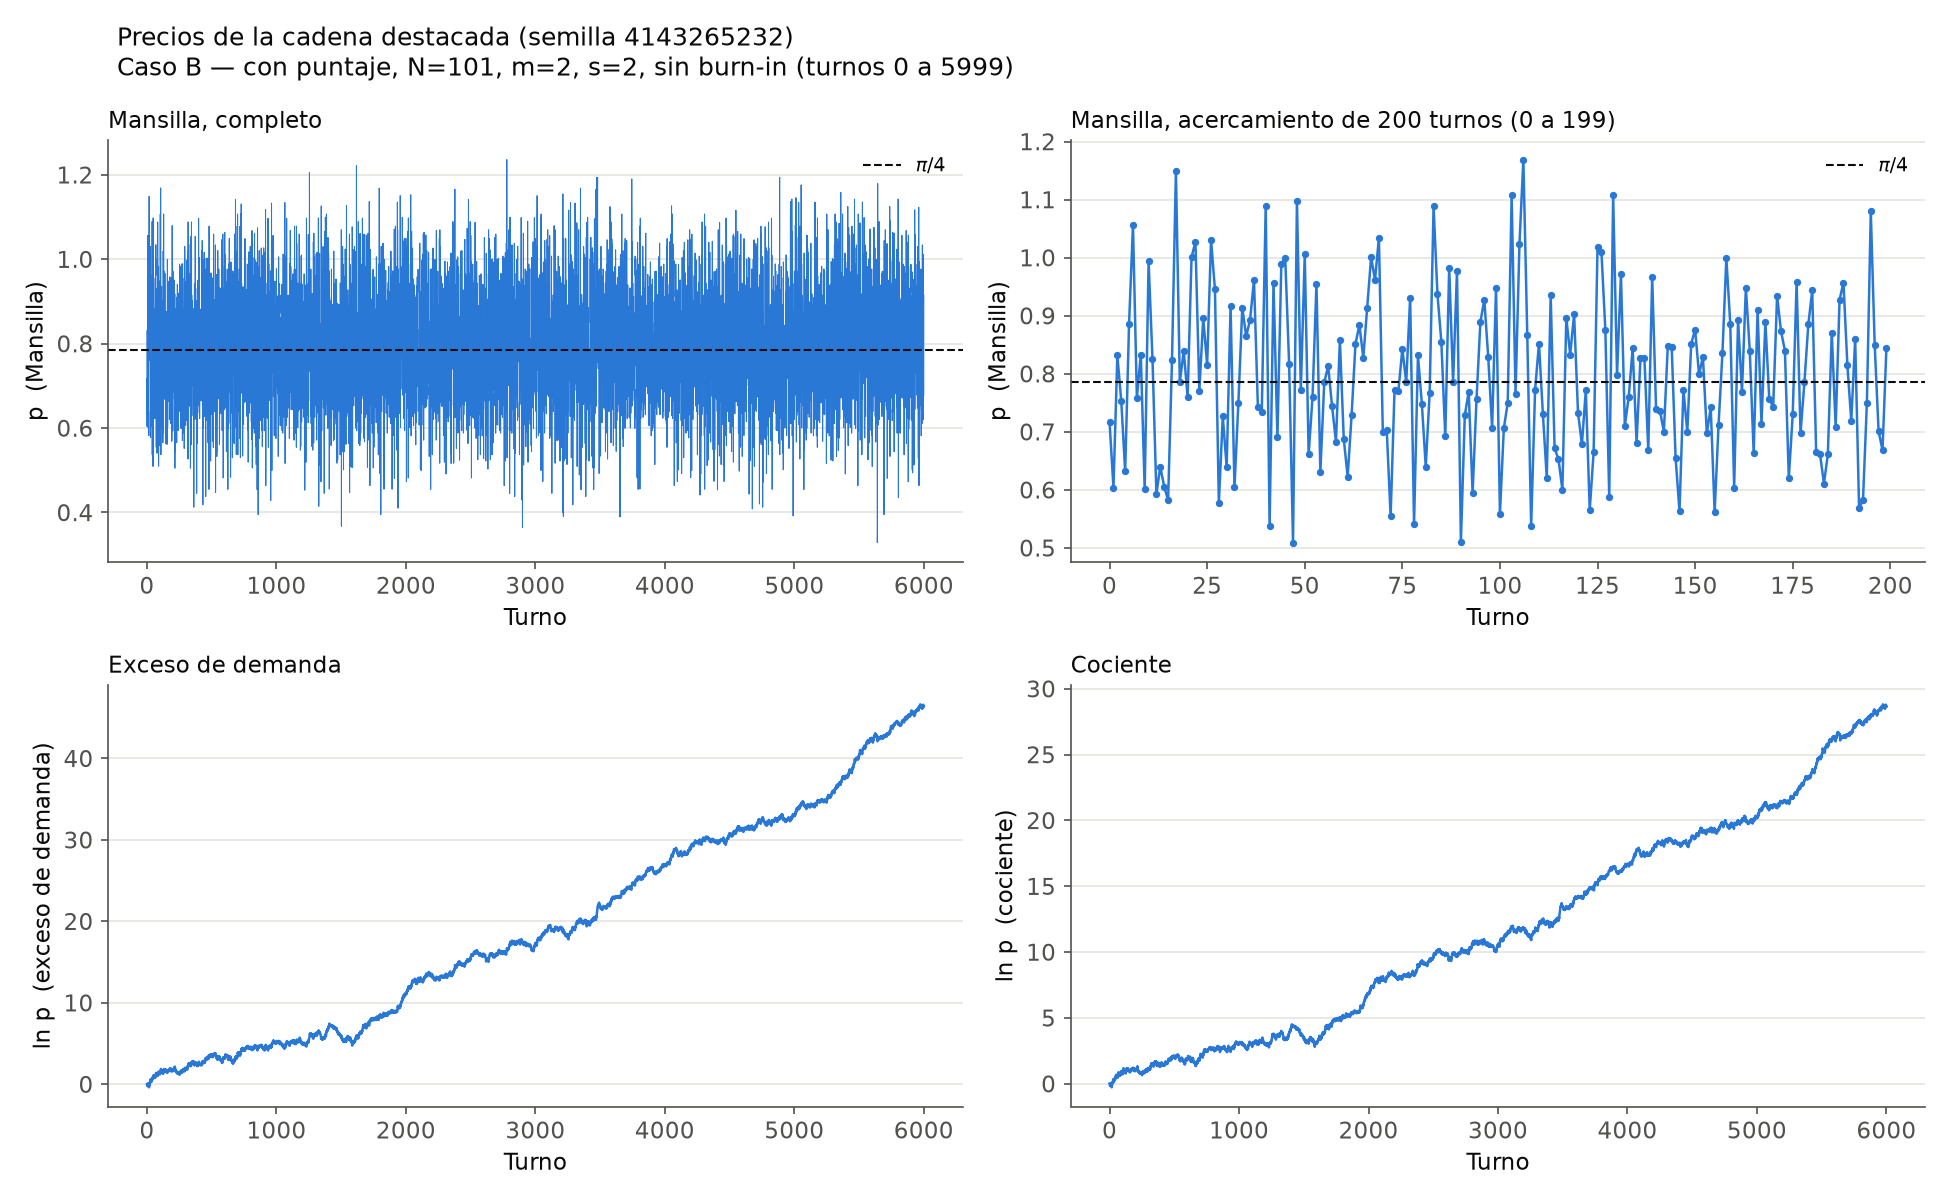
\includegraphics[width=0.49\textwidth]{figuras/Fase9_precios_detalle_casoB_N101_m2_s2_con_puntaje_T6000_regla_nueva_sin_burnin.png}\hfill
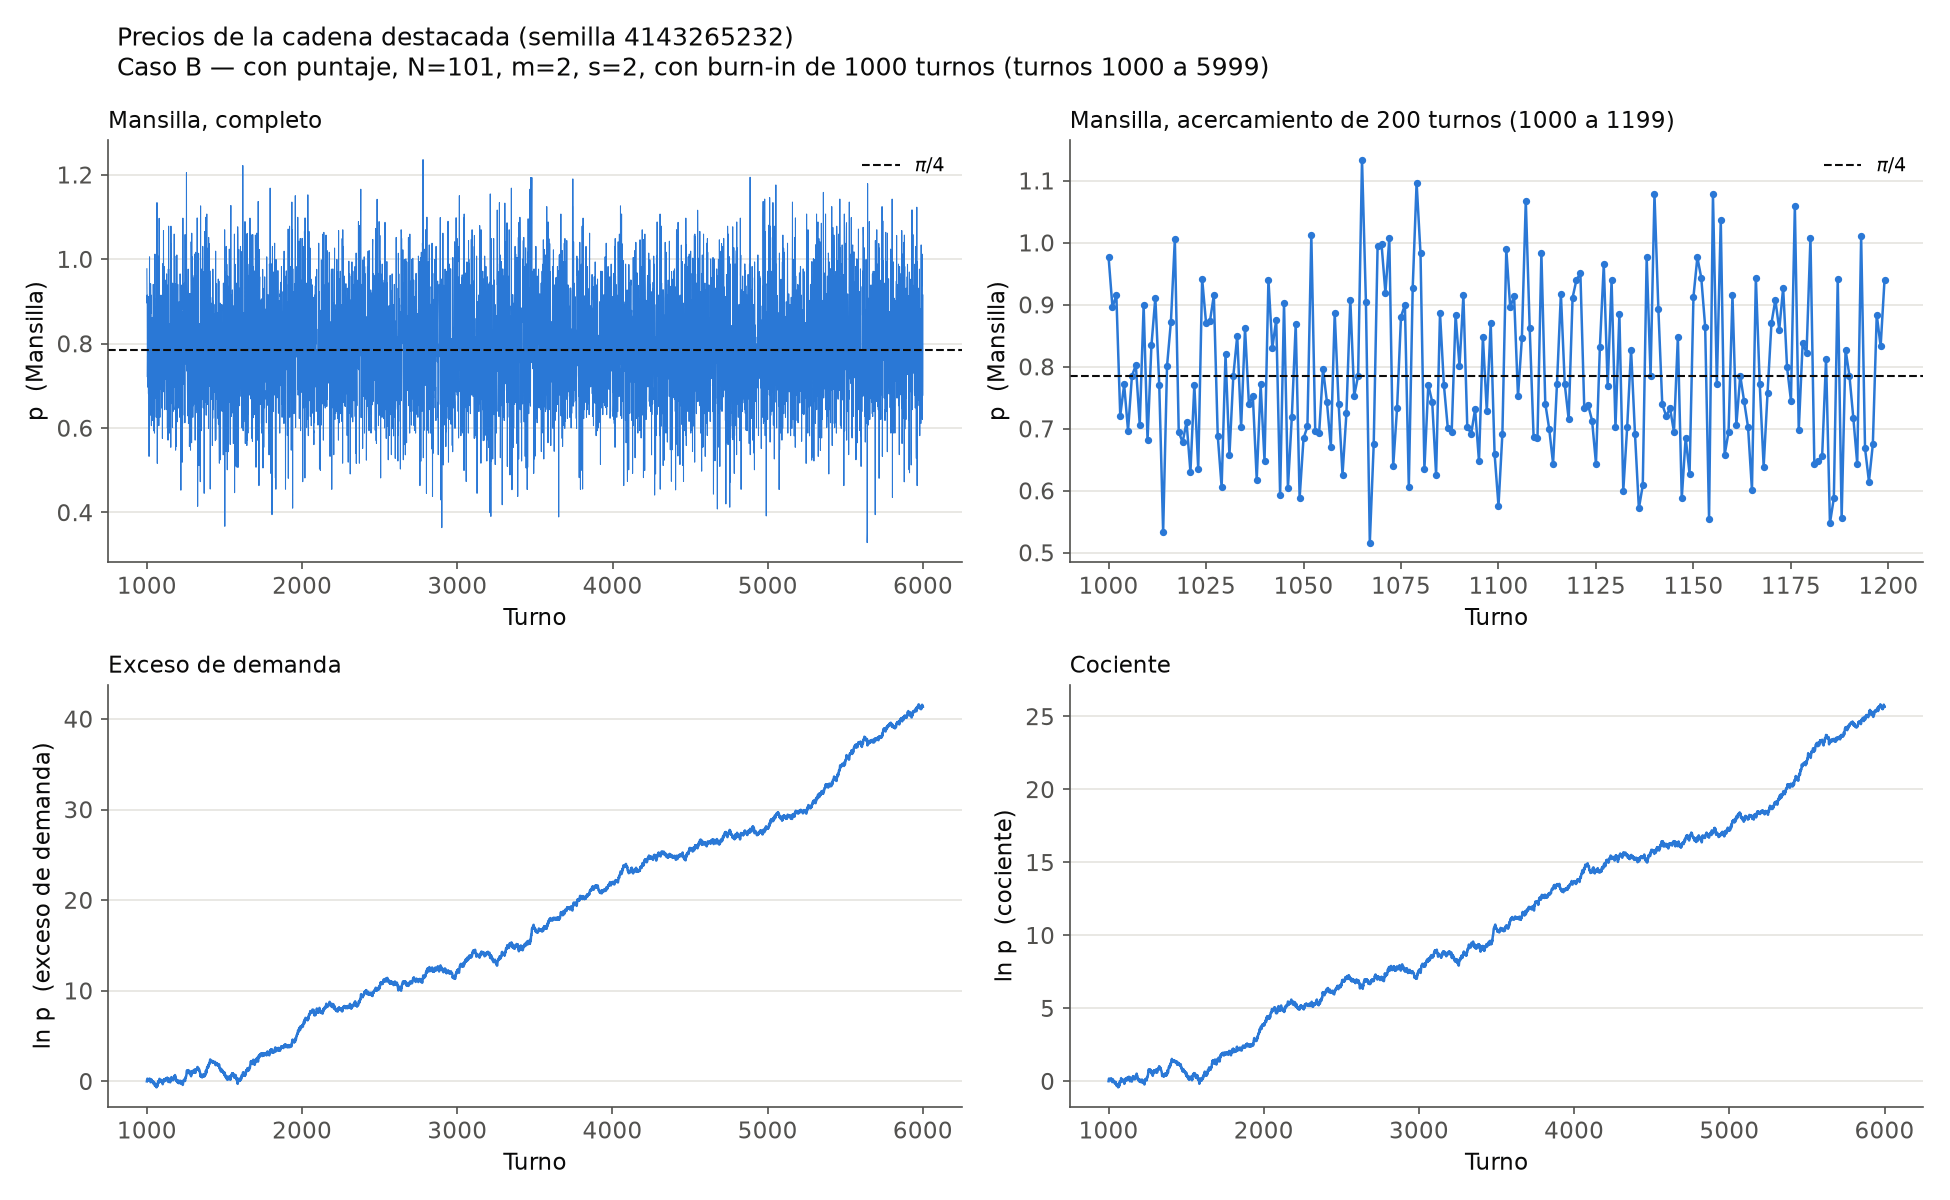
\includegraphics[width=0.49\textwidth]{figuras/Fase9_precios_detalle_casoB_N101_m2_s2_con_puntaje_T6000_regla_nueva_con_burnin1000.png}
\caption{Caso B, $N=101$: detalle de la cadena destacada sin burn-in (izquierda) y con burn-in (derecha).}
\end{figure}

\subsection*{Caso C: $m=3$, sin puntaje}
\begin{figure}[H]
\centering
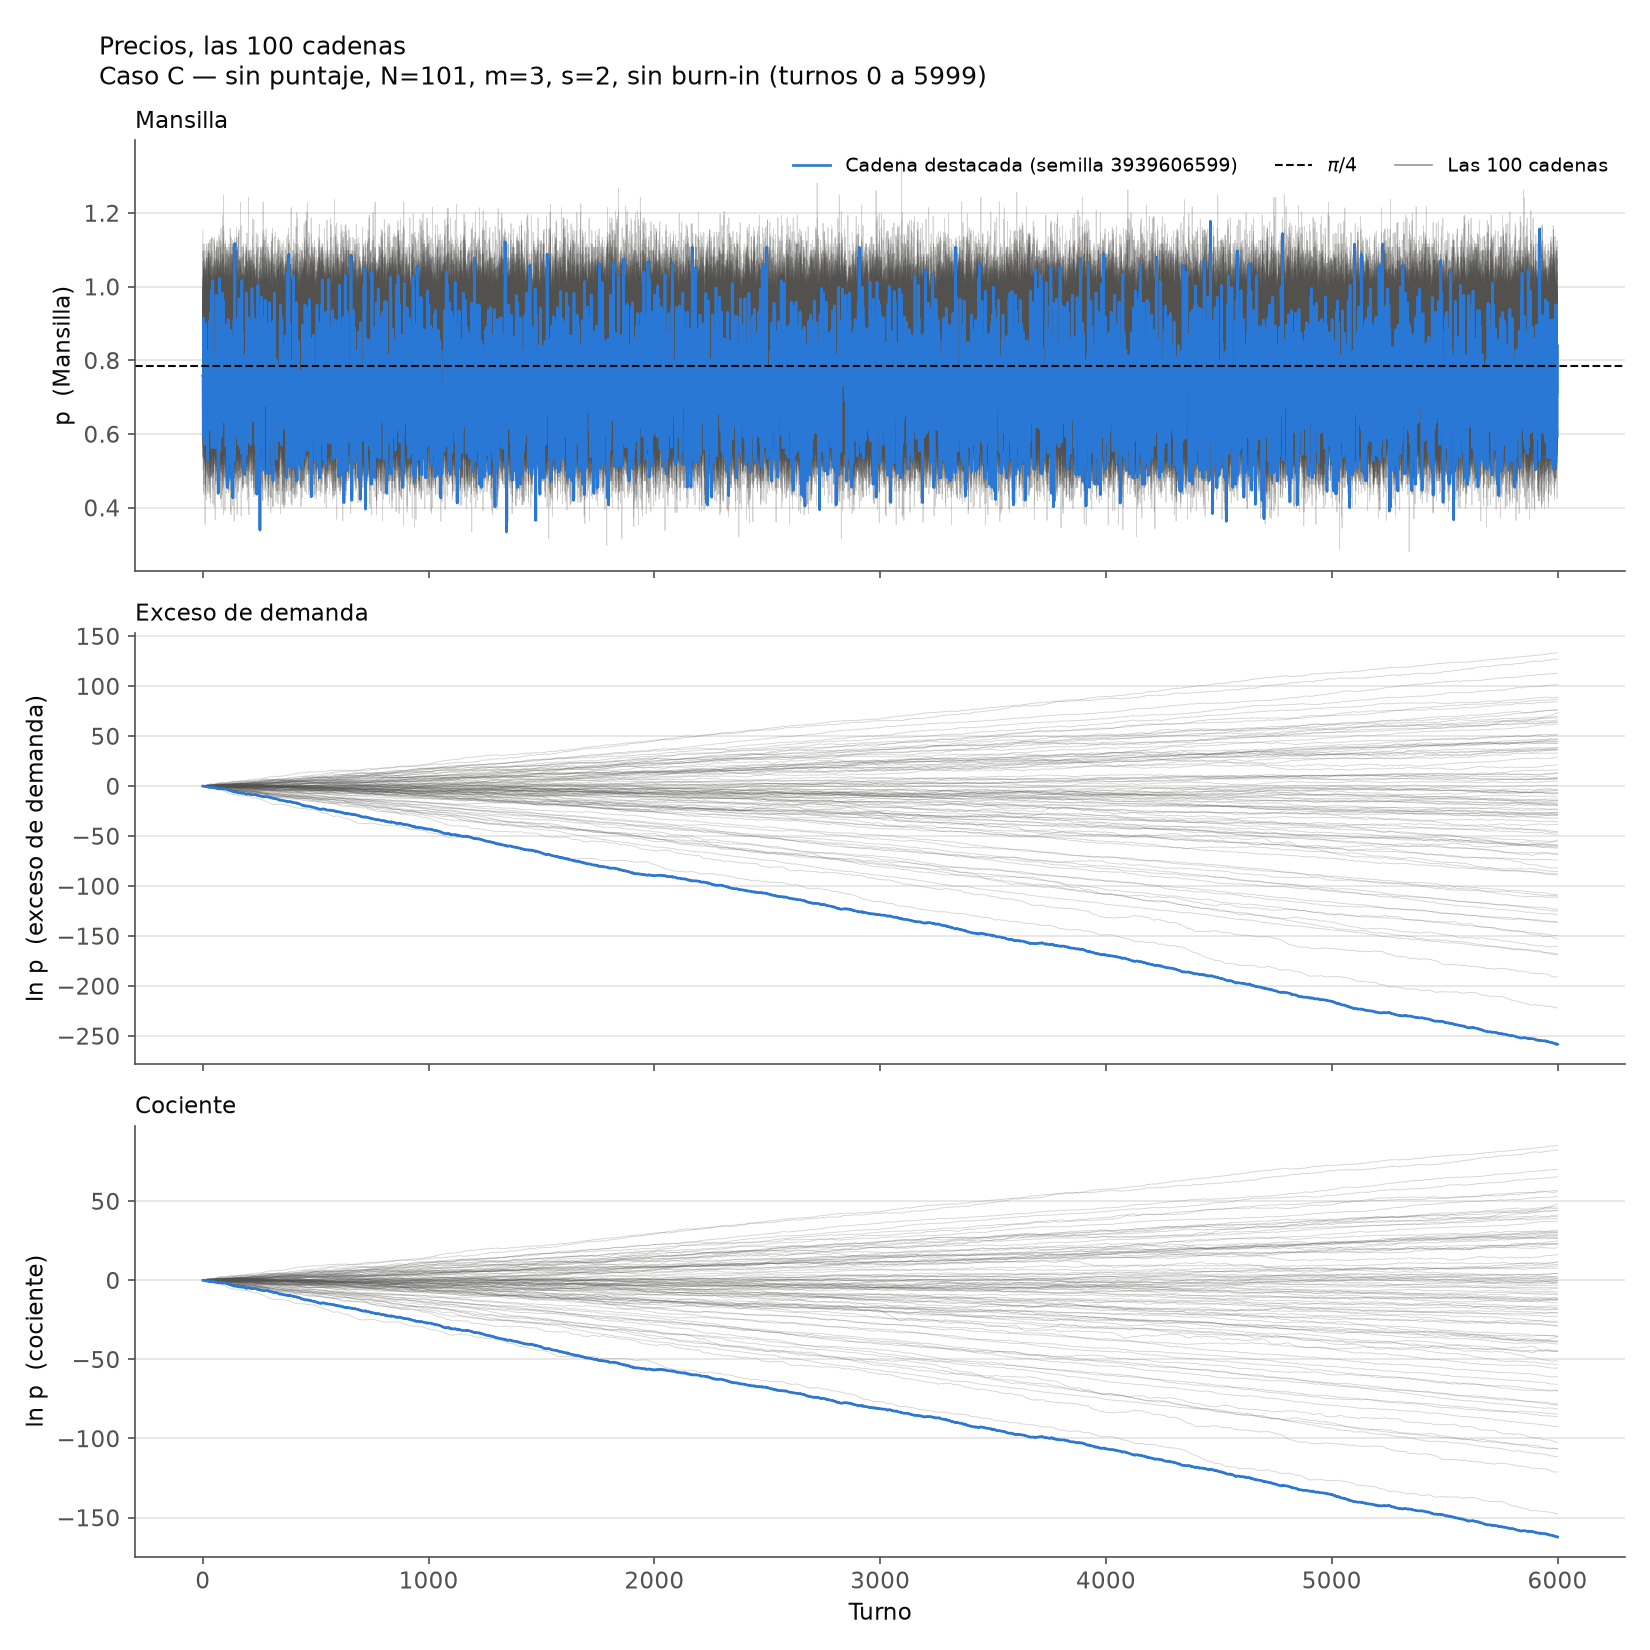
\includegraphics[width=0.49\textwidth]{figuras/Fase9_precios_conjunto_casoC_N101_m3_s2_sin_puntaje_T6000_regla_nueva_sin_burnin.png}\hfill
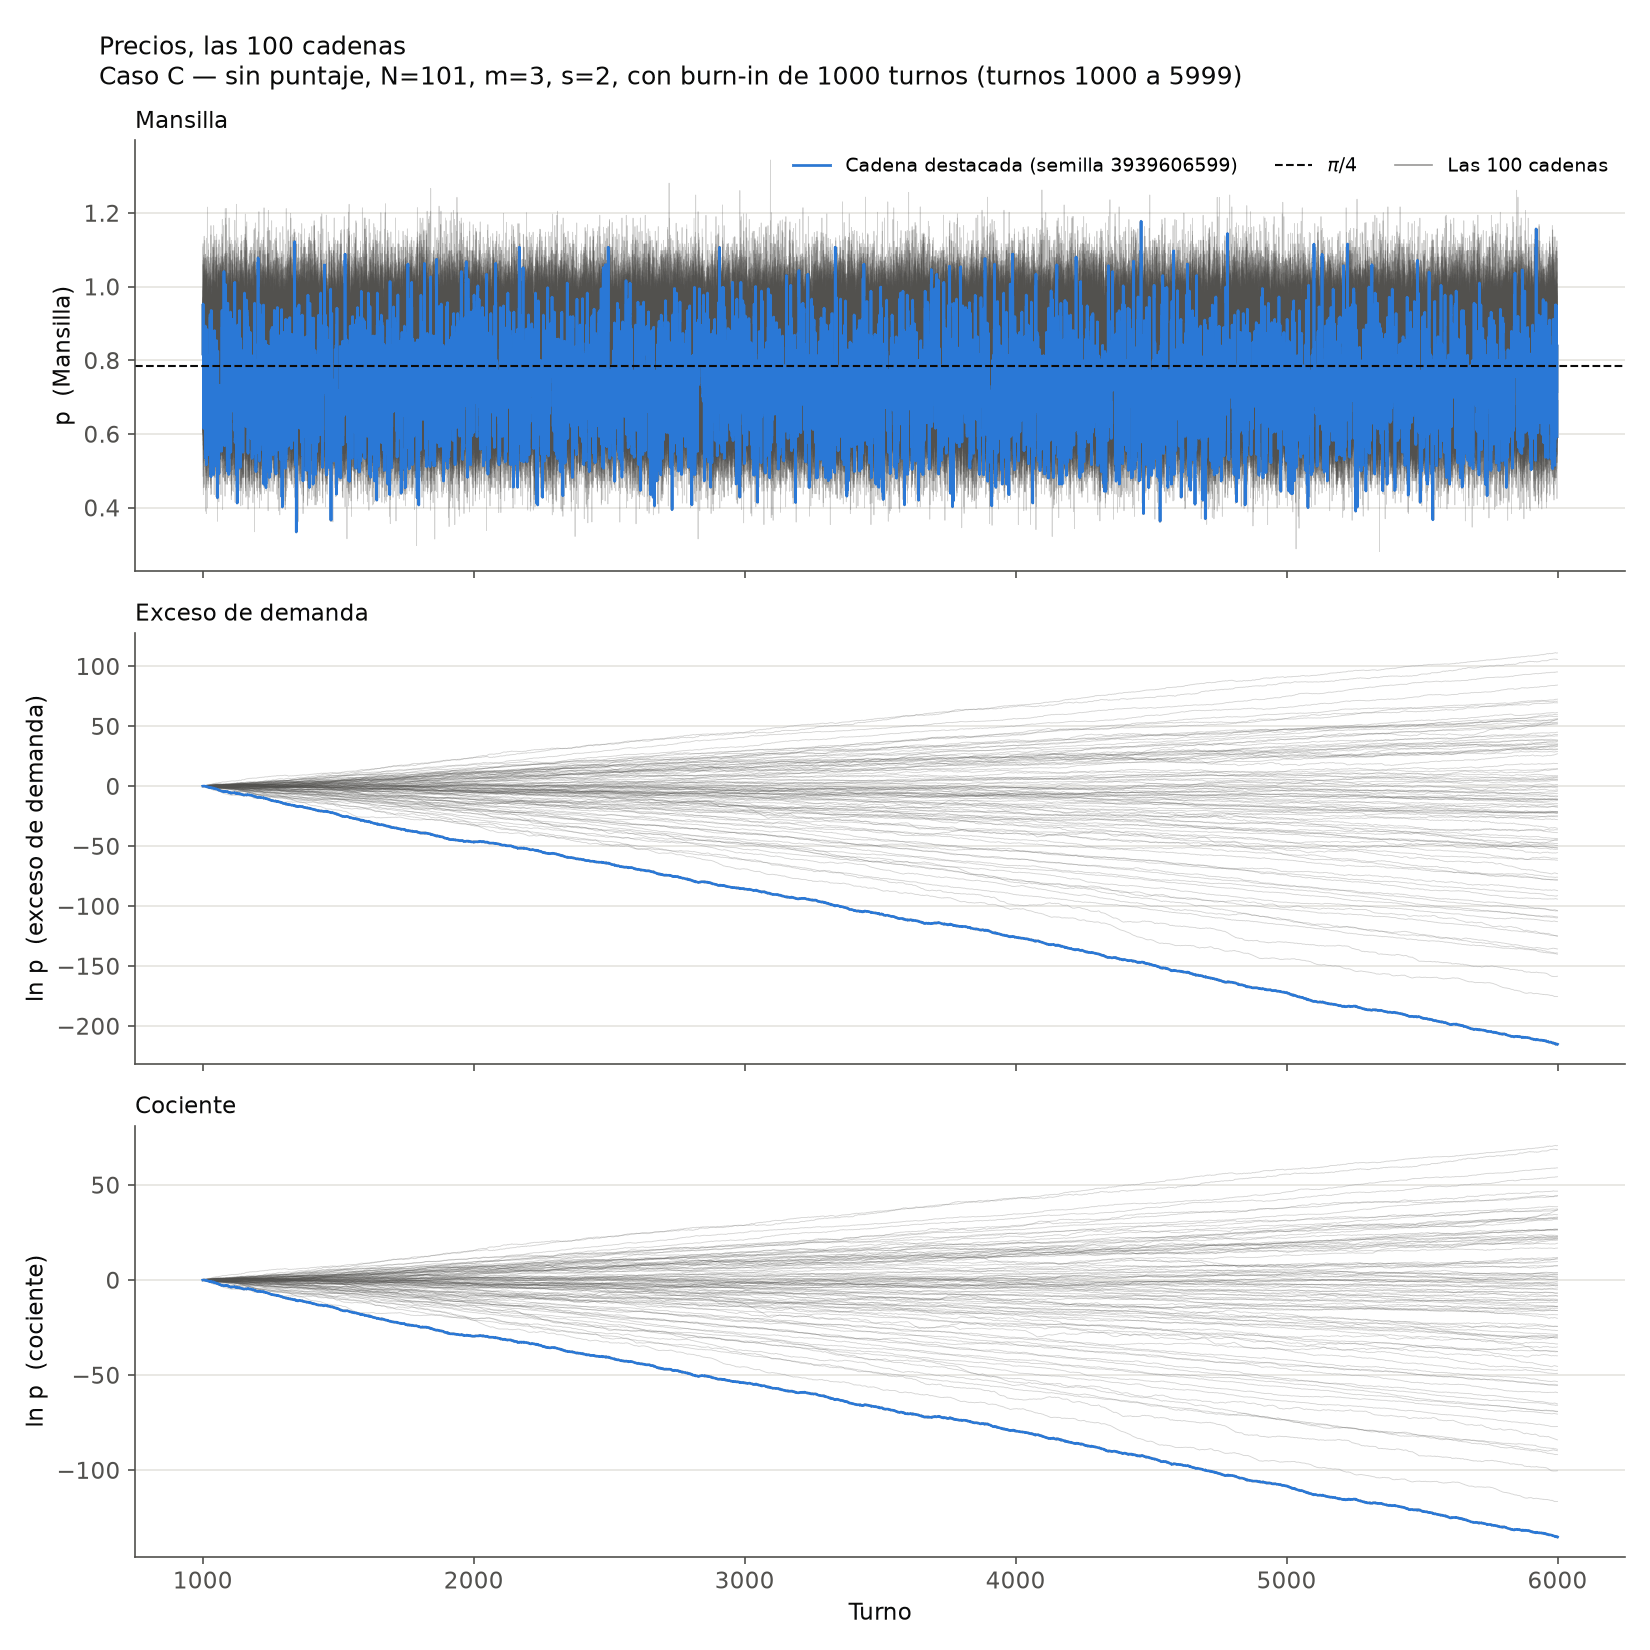
\includegraphics[width=0.49\textwidth]{figuras/Fase9_precios_conjunto_casoC_N101_m3_s2_sin_puntaje_T6000_regla_nueva_con_burnin1000.png}
\caption{Caso C, $N=101$: conjunto de precios sin burn-in (izquierda) y con burn-in de 1000 turnos (derecha).}
\end{figure}

\begin{figure}[H]
\centering
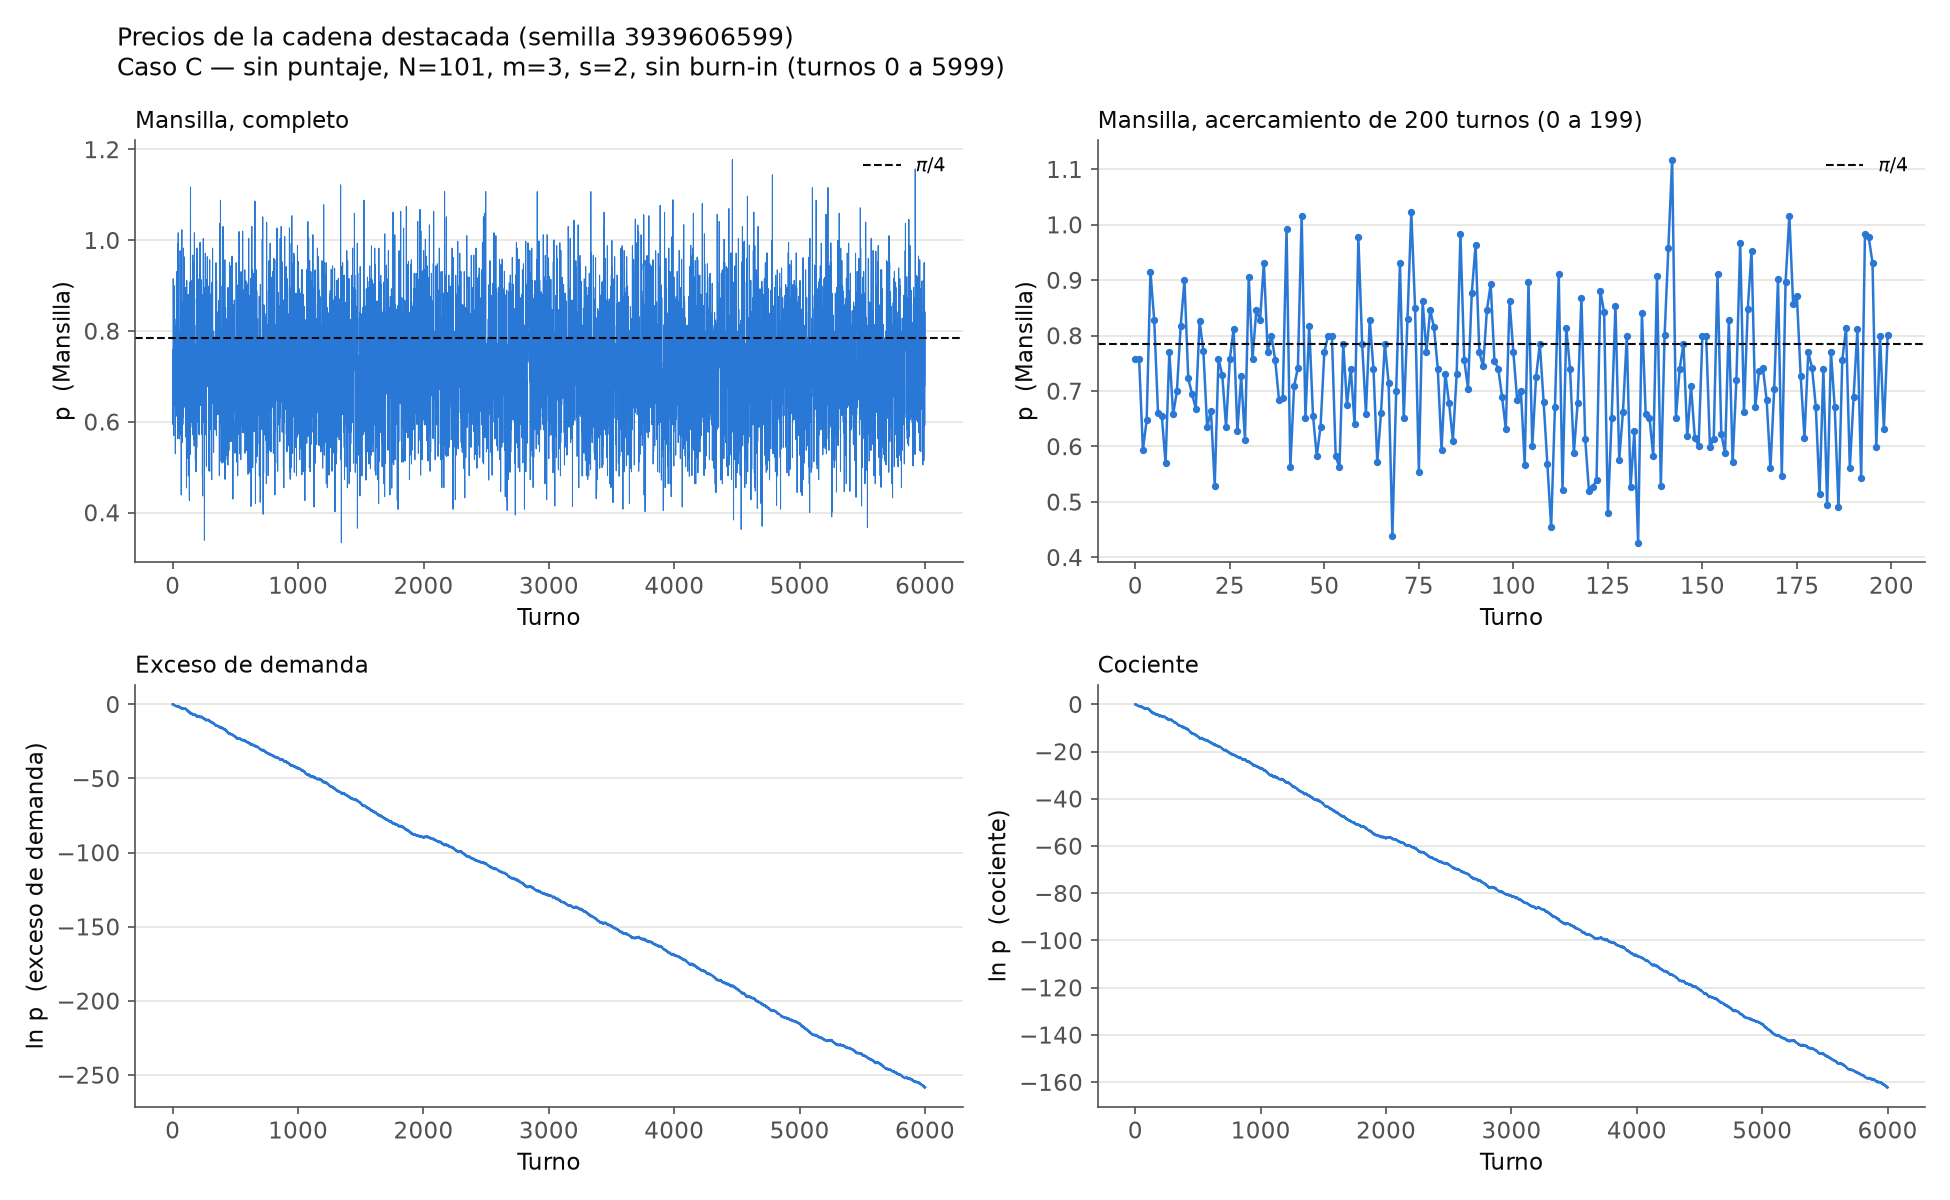
\includegraphics[width=0.49\textwidth]{figuras/Fase9_precios_detalle_casoC_N101_m3_s2_sin_puntaje_T6000_regla_nueva_sin_burnin.png}\hfill
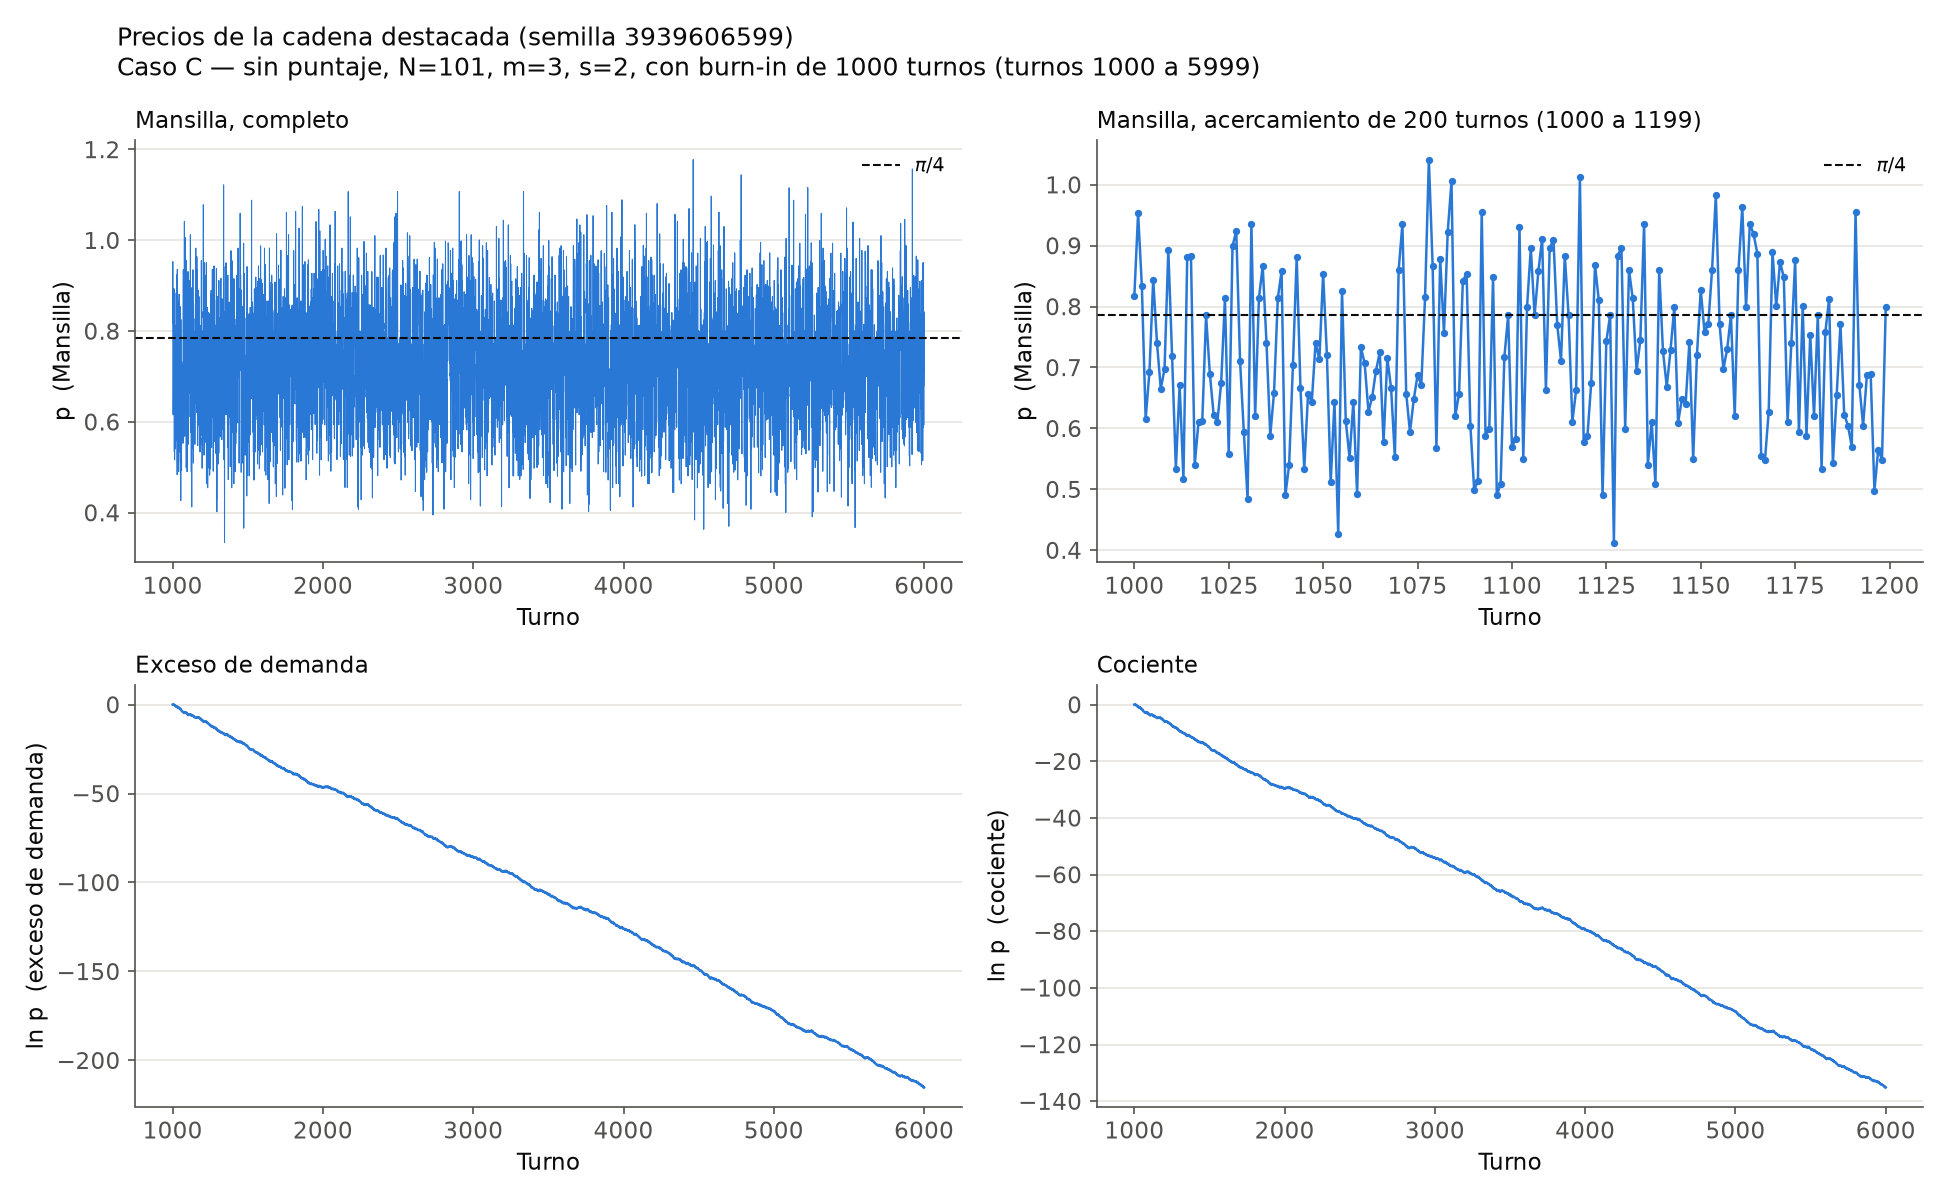
\includegraphics[width=0.49\textwidth]{figuras/Fase9_precios_detalle_casoC_N101_m3_s2_sin_puntaje_T6000_regla_nueva_con_burnin1000.png}
\caption{Caso C, $N=101$: detalle de la cadena destacada sin burn-in (izquierda) y con burn-in (derecha).}
\end{figure}

\subsection*{Caso D: $m=3$, con puntaje}
\begin{figure}[H]
\centering
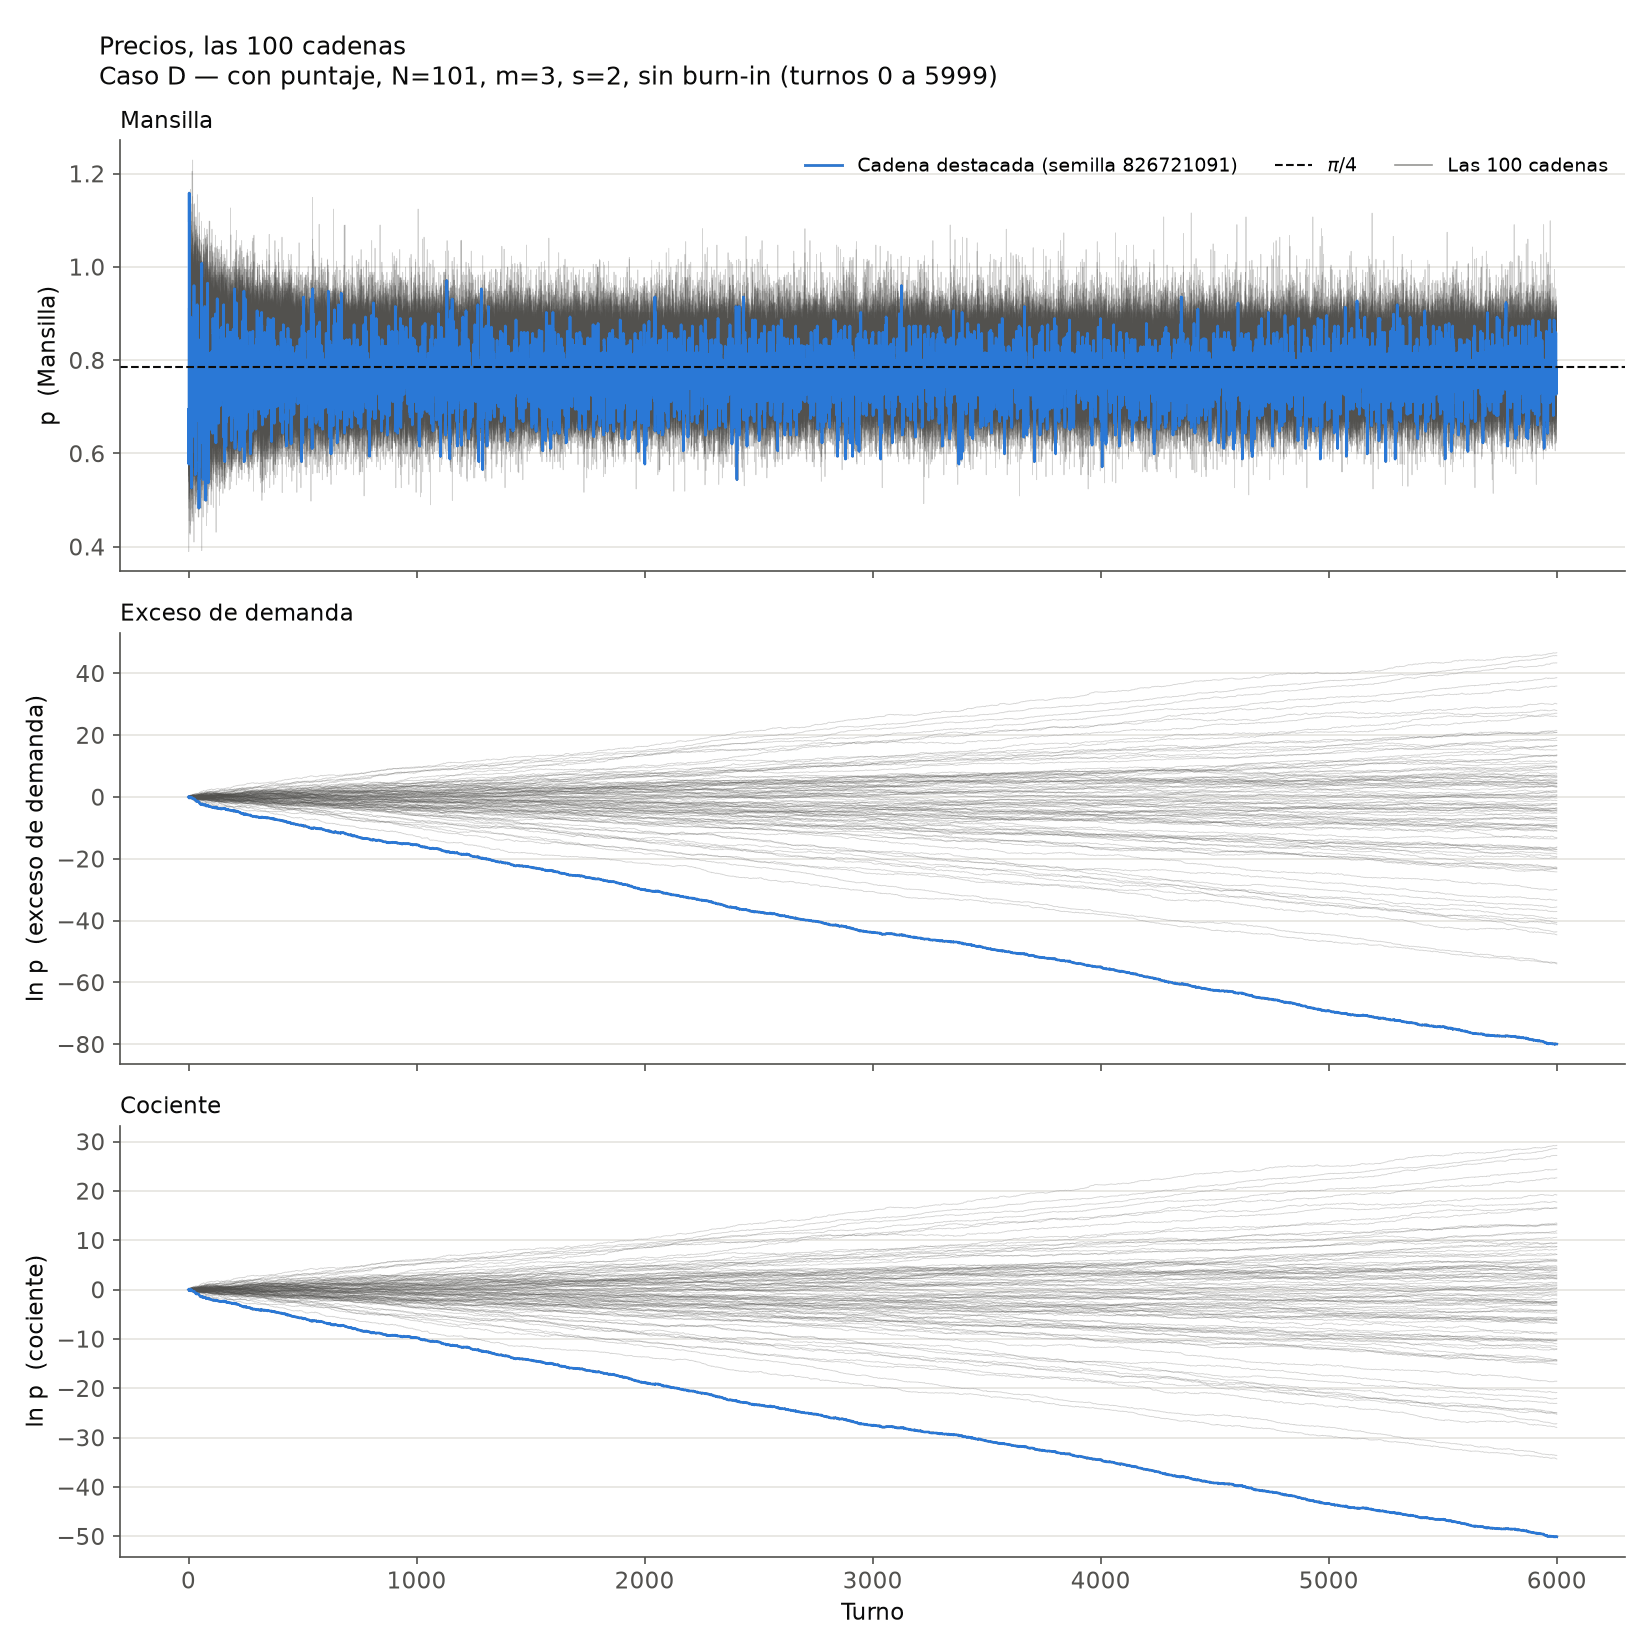
\includegraphics[width=0.49\textwidth]{figuras/Fase9_precios_conjunto_casoD_N101_m3_s2_con_puntaje_T6000_regla_nueva_sin_burnin.png}\hfill
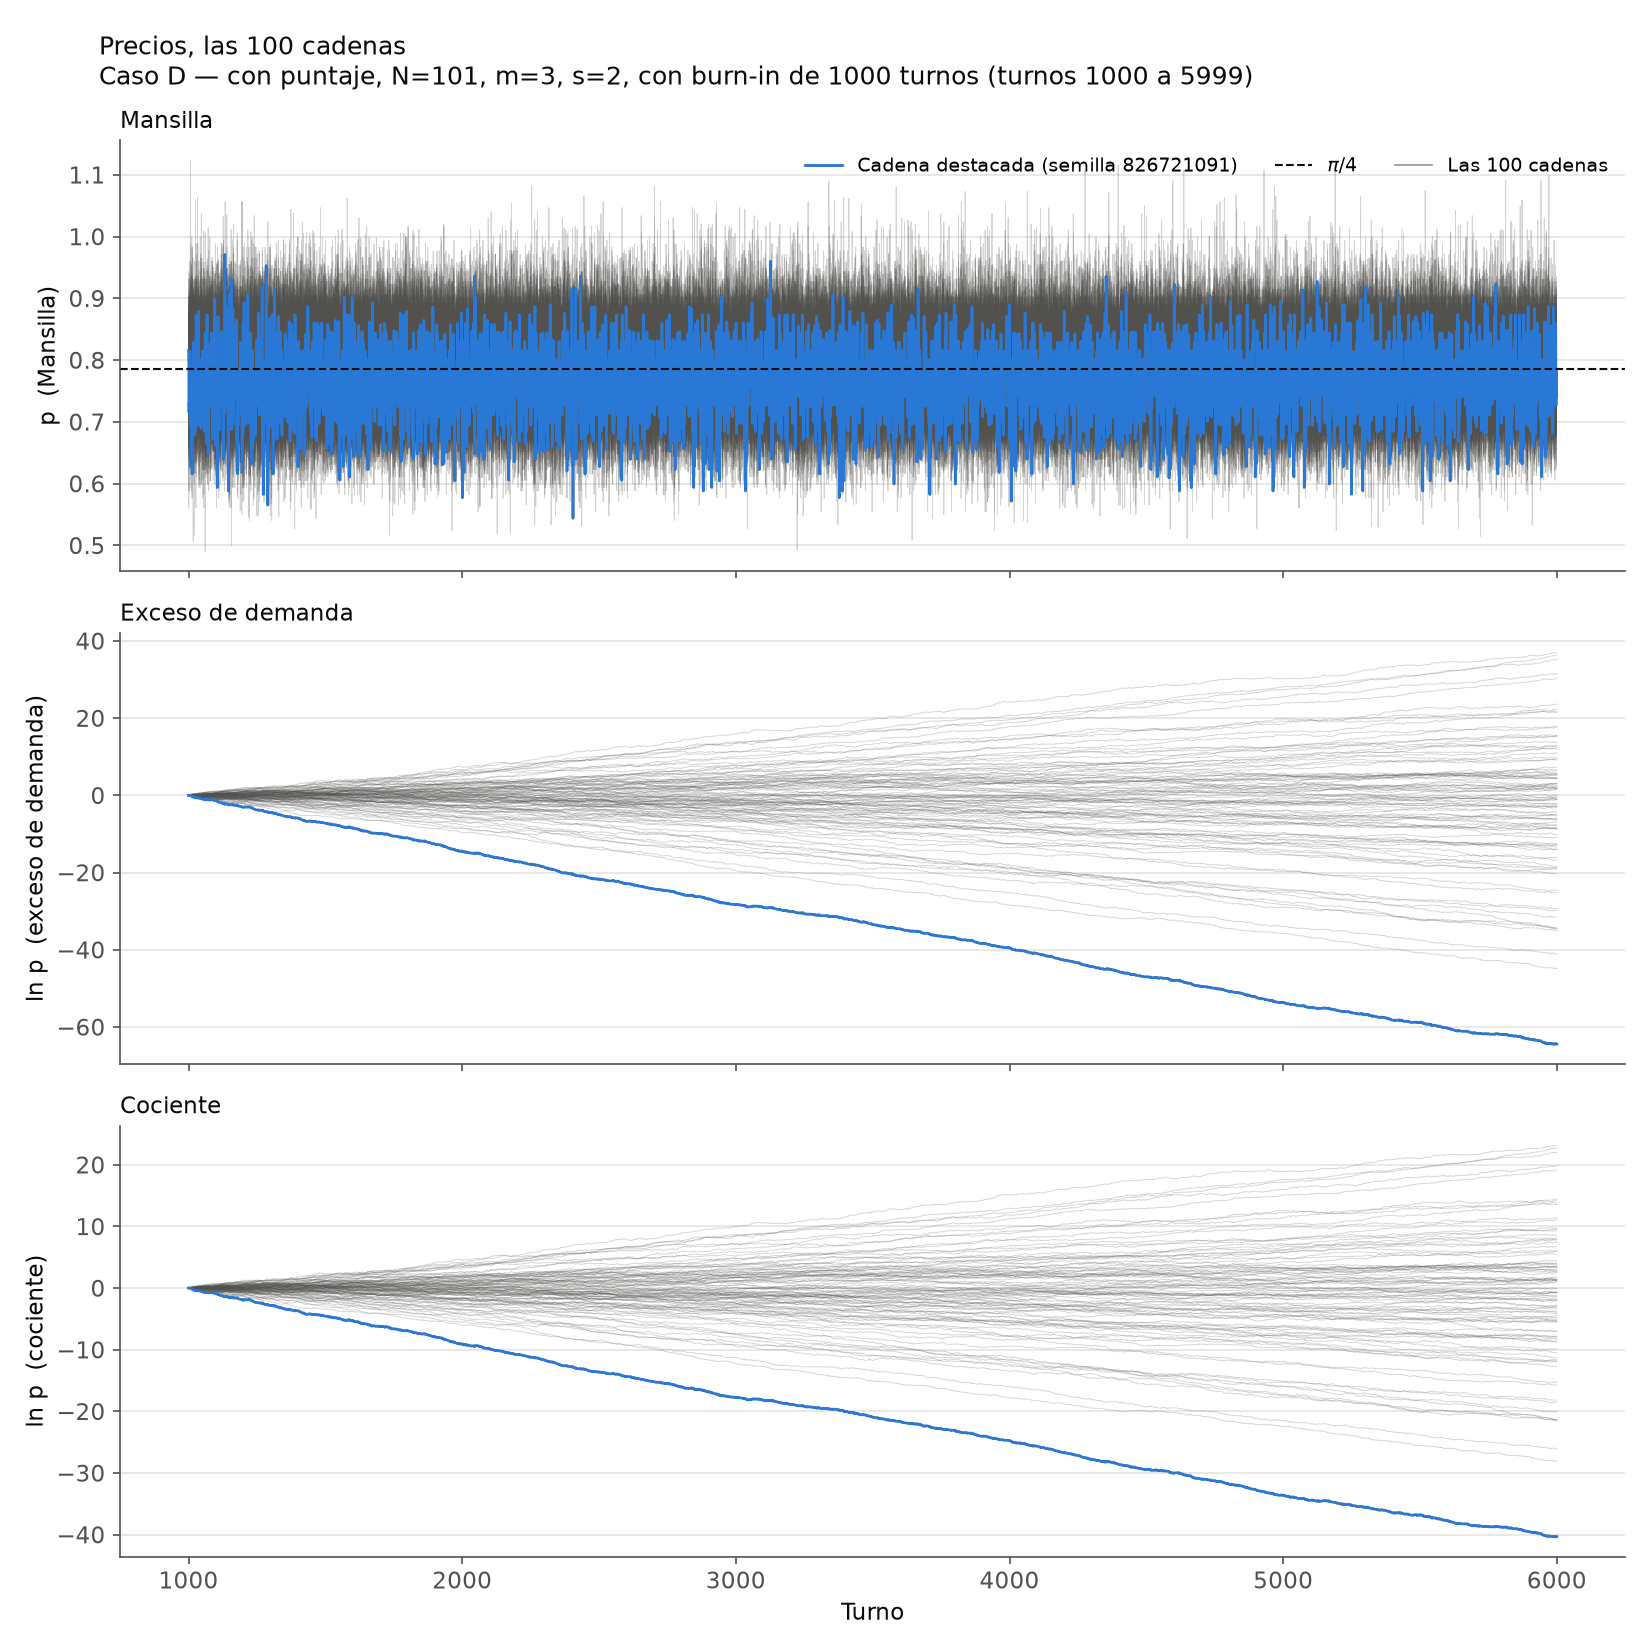
\includegraphics[width=0.49\textwidth]{figuras/Fase9_precios_conjunto_casoD_N101_m3_s2_con_puntaje_T6000_regla_nueva_con_burnin1000.png}
\caption{Caso D, $N=101$: conjunto de precios sin burn-in (izquierda) y con burn-in de 1000 turnos (derecha).}
\end{figure}

\begin{figure}[H]
\centering
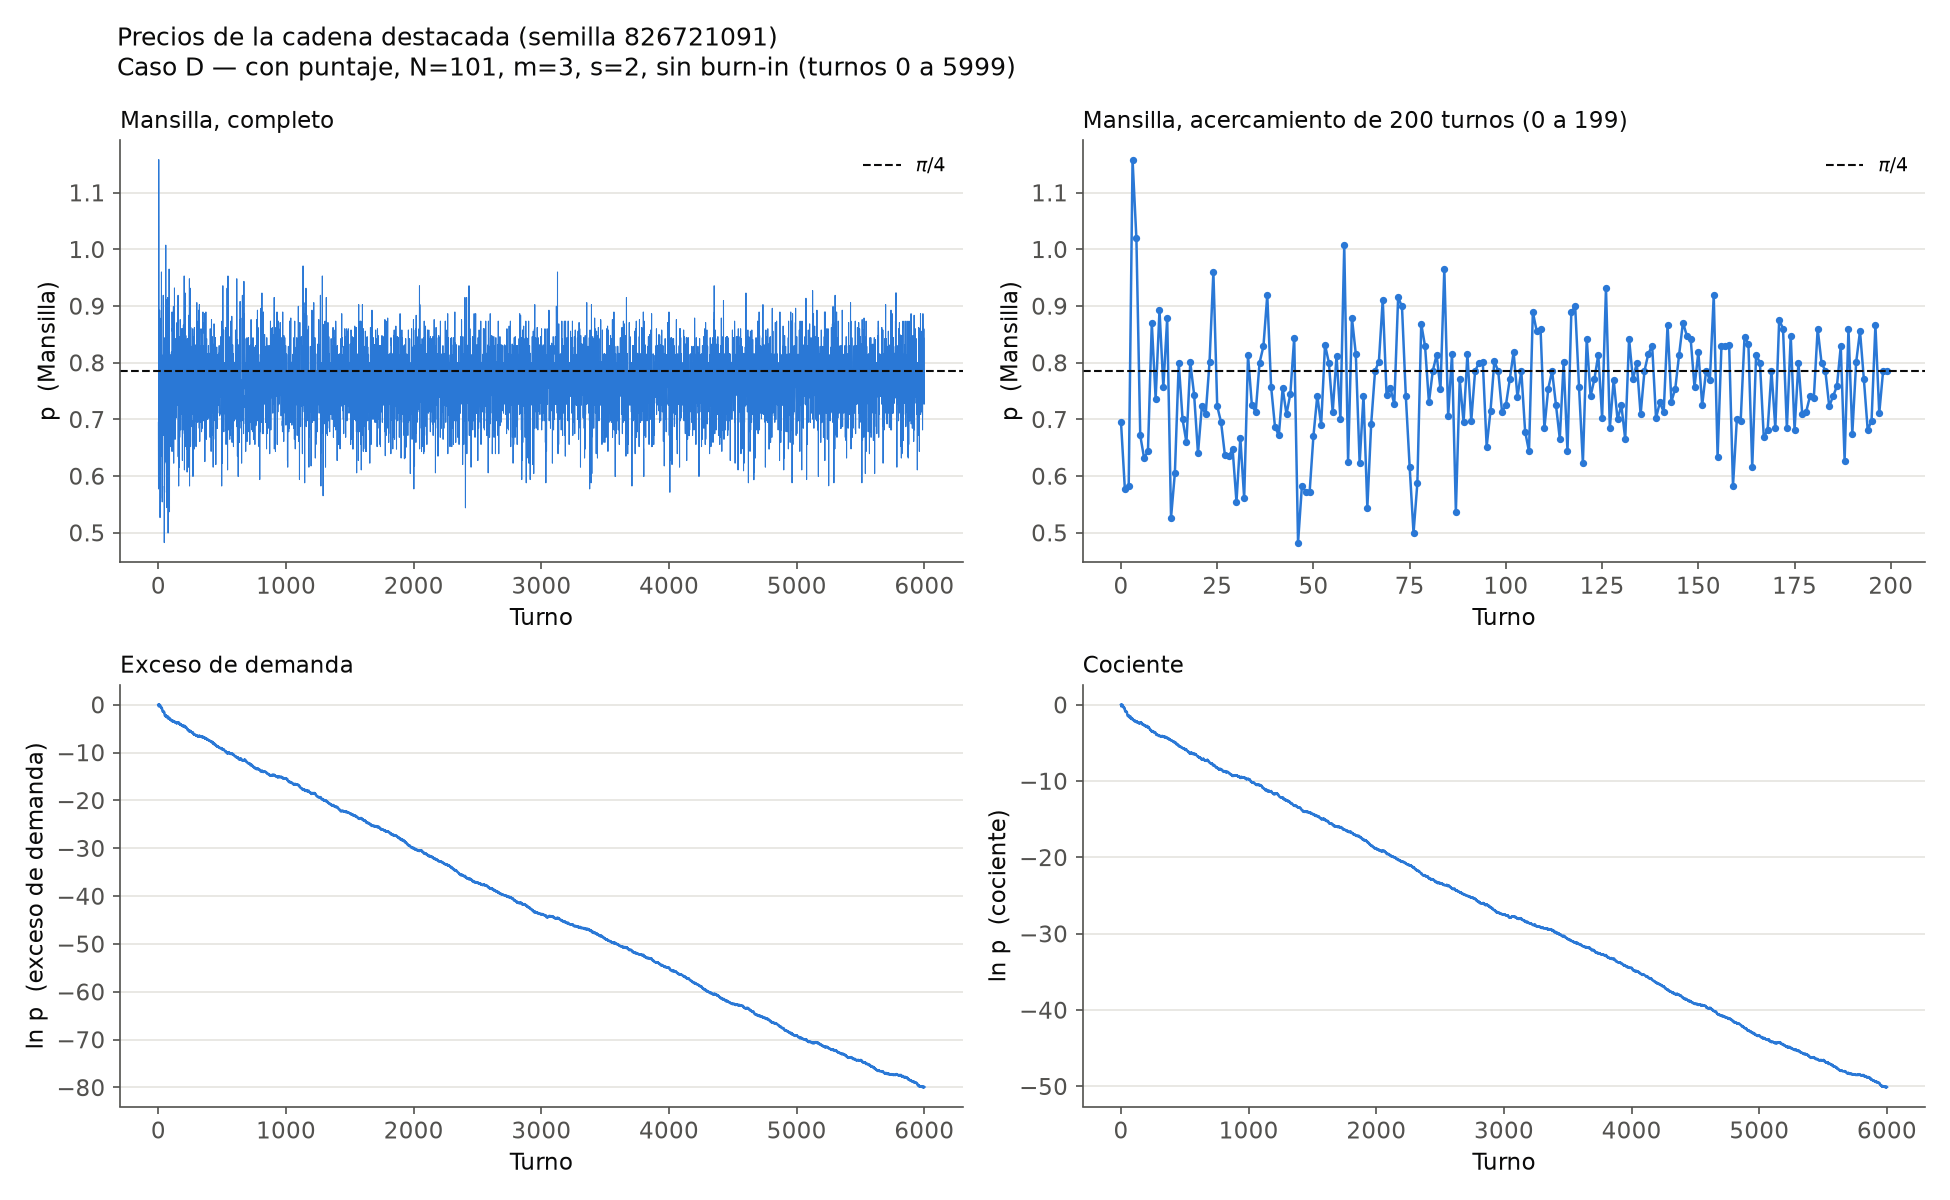
\includegraphics[width=0.49\textwidth]{figuras/Fase9_precios_detalle_casoD_N101_m3_s2_con_puntaje_T6000_regla_nueva_sin_burnin.png}\hfill
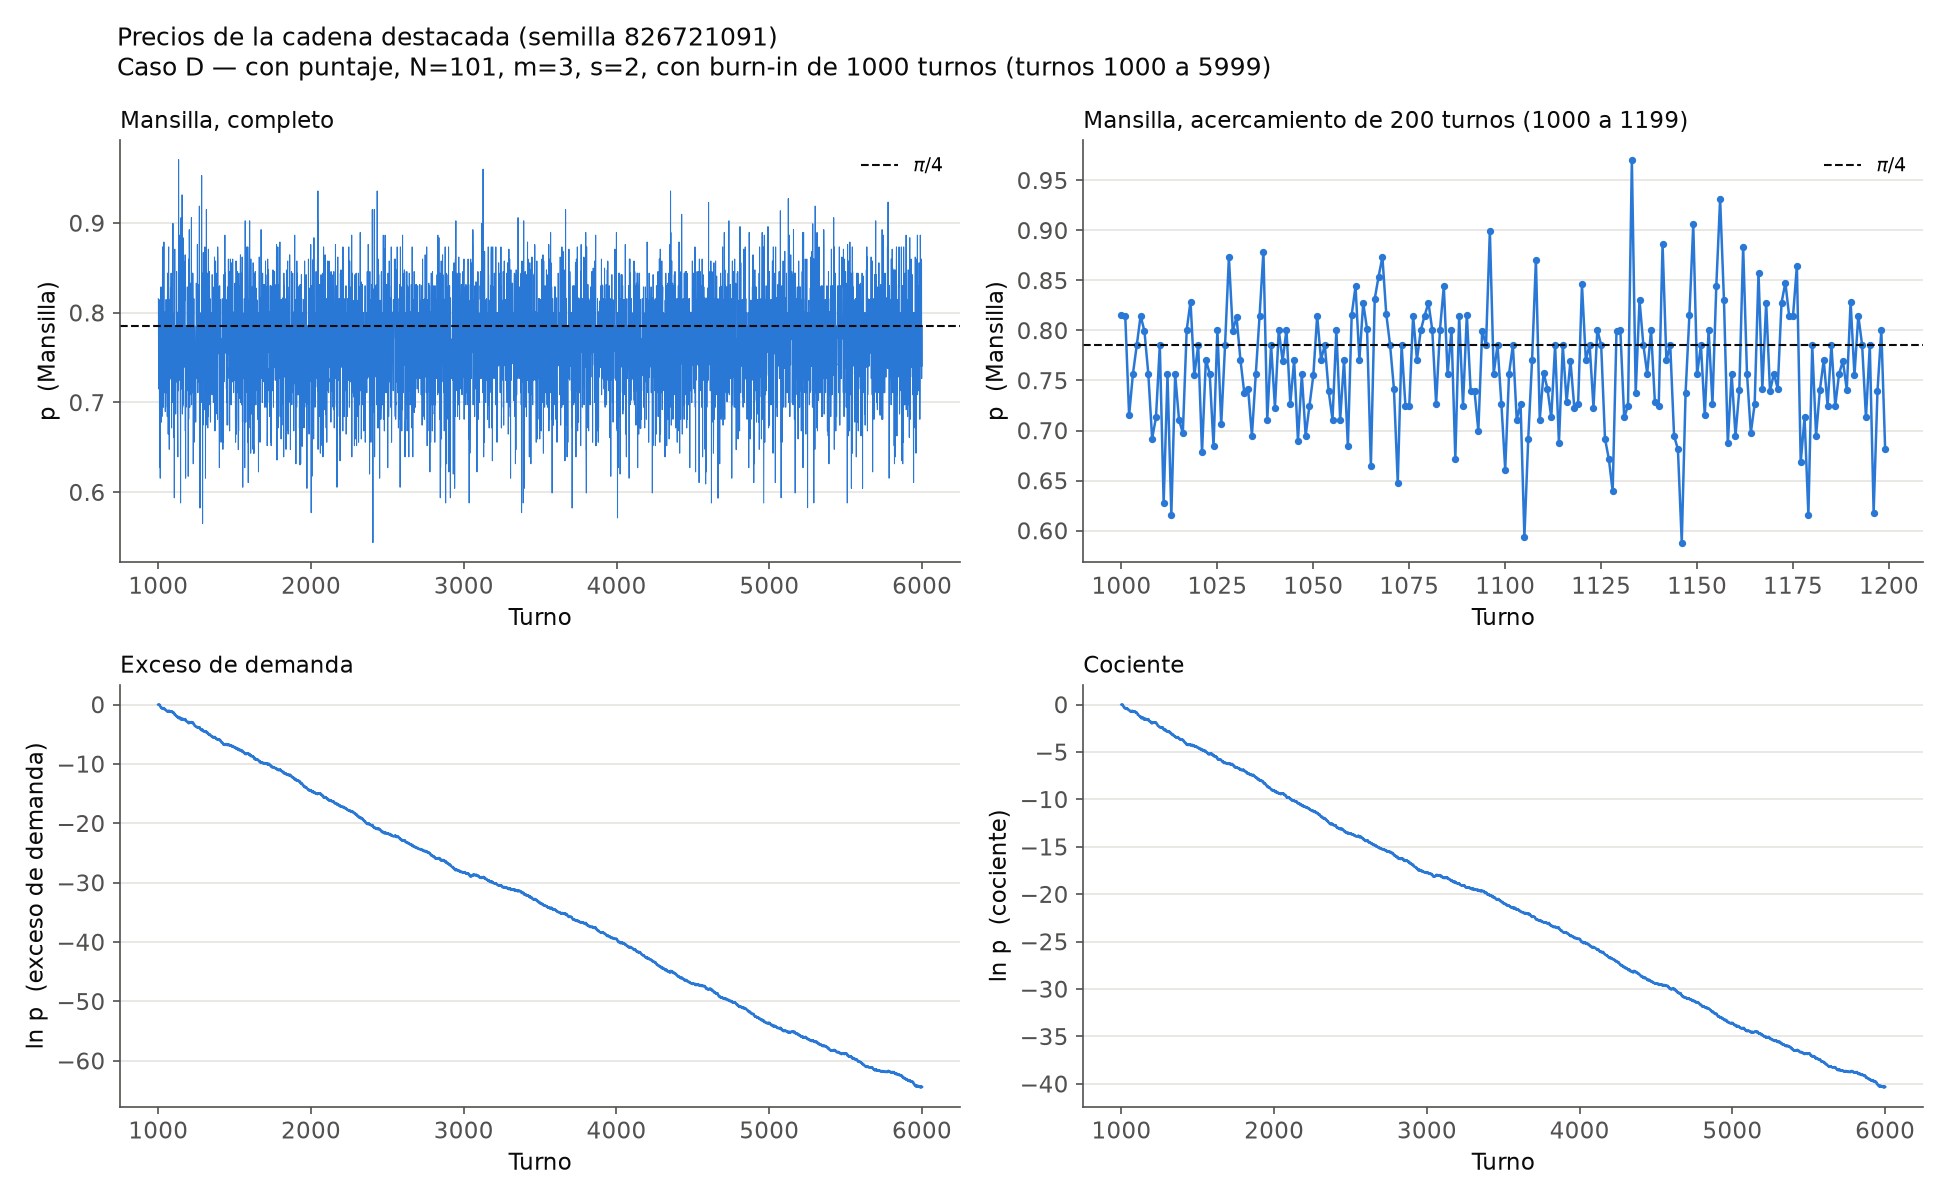
\includegraphics[width=0.49\textwidth]{figuras/Fase9_precios_detalle_casoD_N101_m3_s2_con_puntaje_T6000_regla_nueva_con_burnin1000.png}
\caption{Caso D, $N=101$: detalle de la cadena destacada sin burn-in (izquierda) y con burn-in (derecha).}
\end{figure}


\section{Fase 9, $N=10000$: gráficas por caso}\label{ap:f9n10000}
Para cada caso: precios (conjunto y detalle, sin y con burn-in), series de rendimientos, volatilidad y abstención de la cadena destacada, hechos estilizados (distribución de $r$ y autocorrelación de $|r|$) y medidas informacionales.
\subsection{Caso A: $m=2$, sin puntaje}
\begin{figure}[H]
\centering
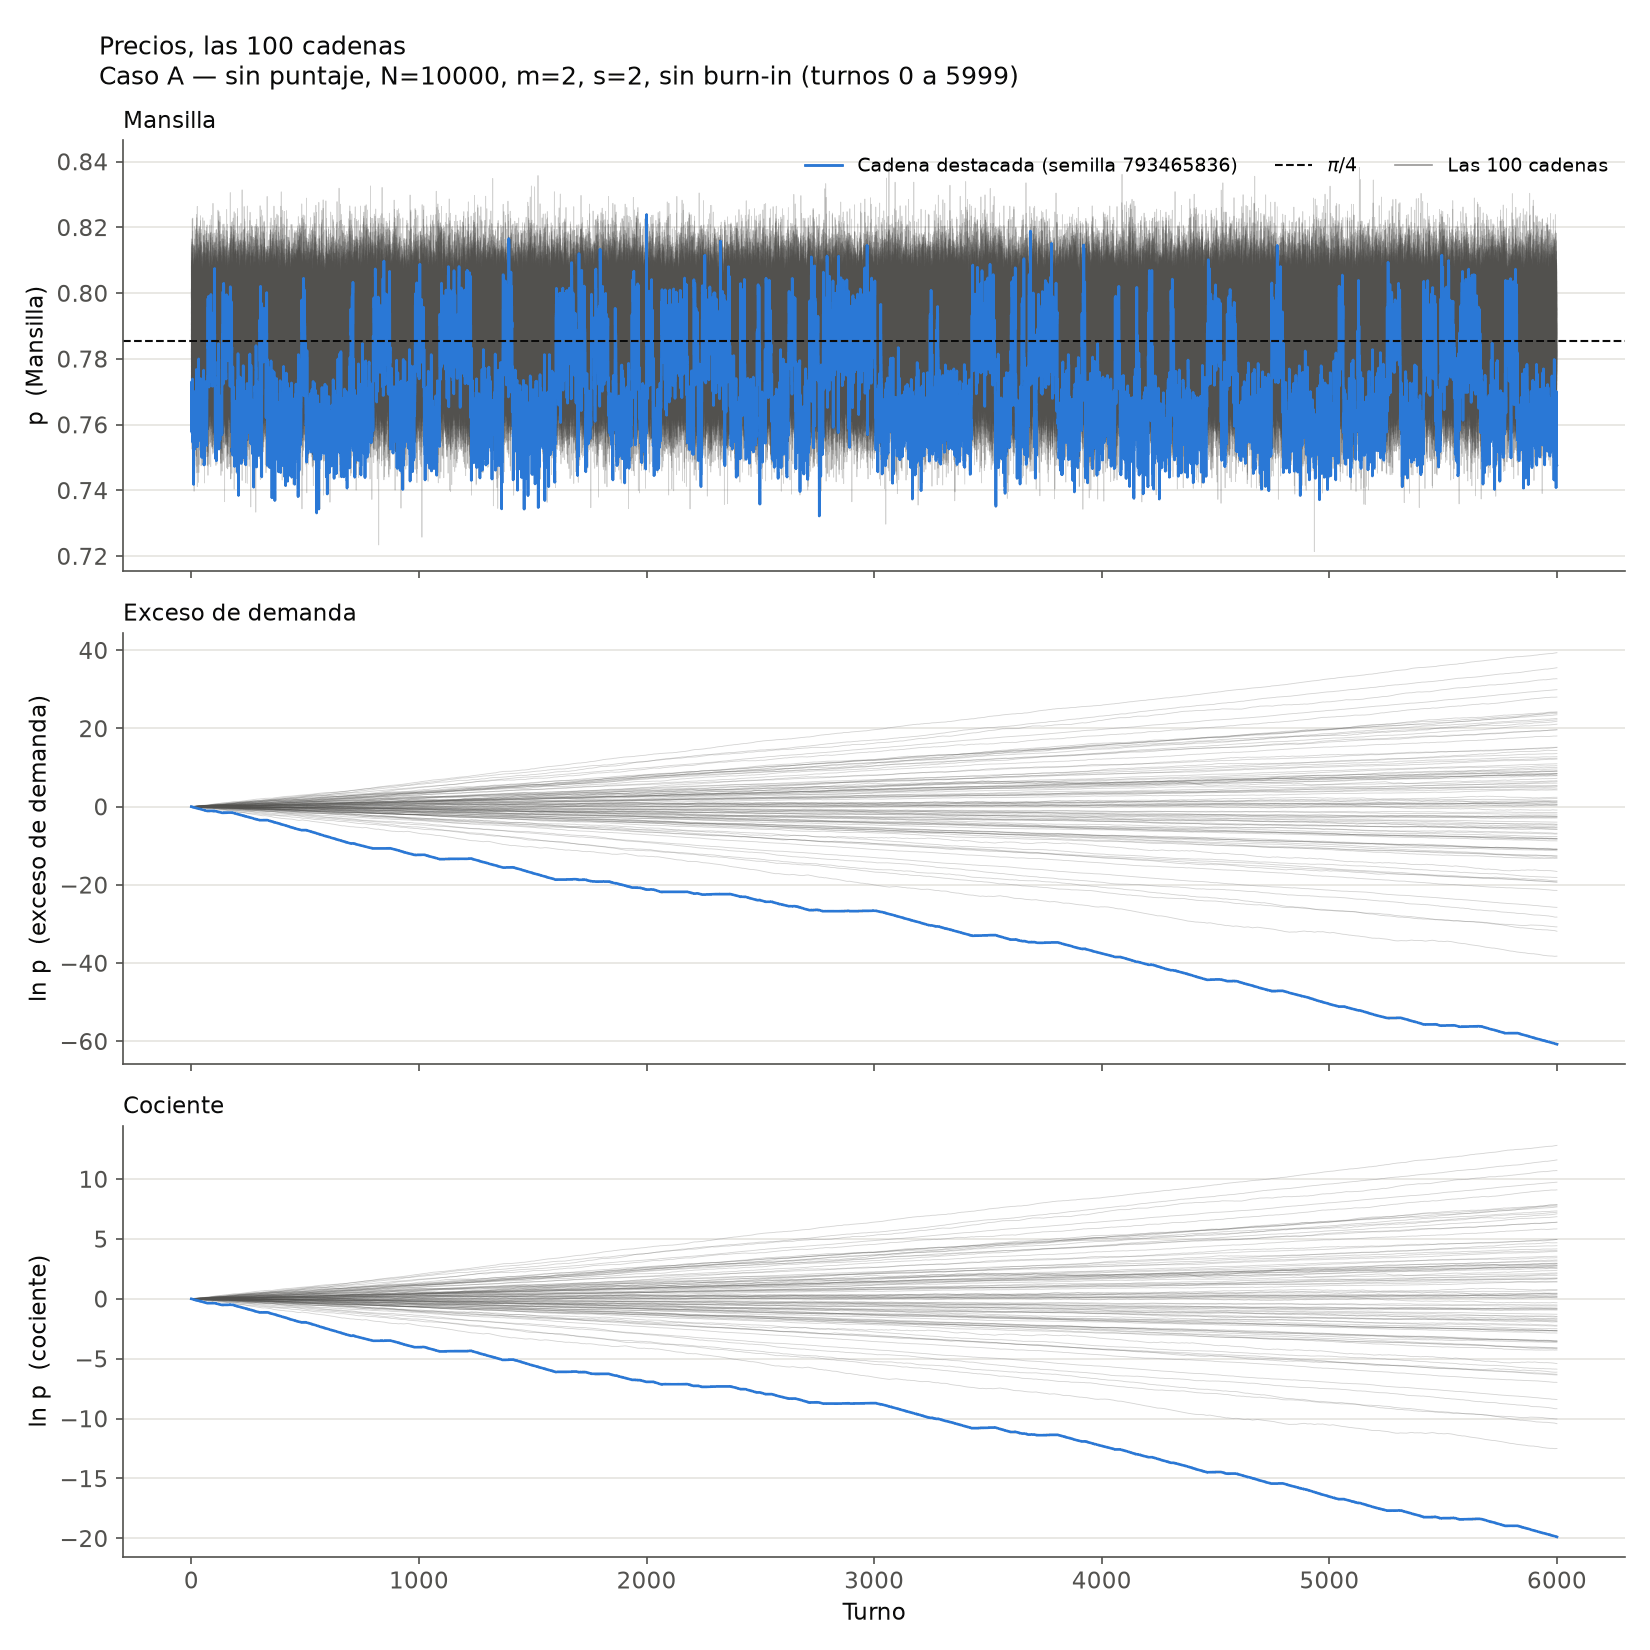
\includegraphics[width=0.49\textwidth]{figuras/Fase9_precios_conjunto_casoA_N10000_m2_s2_sin_puntaje_T6000_regla_nueva_sin_burnin.png}\hfill
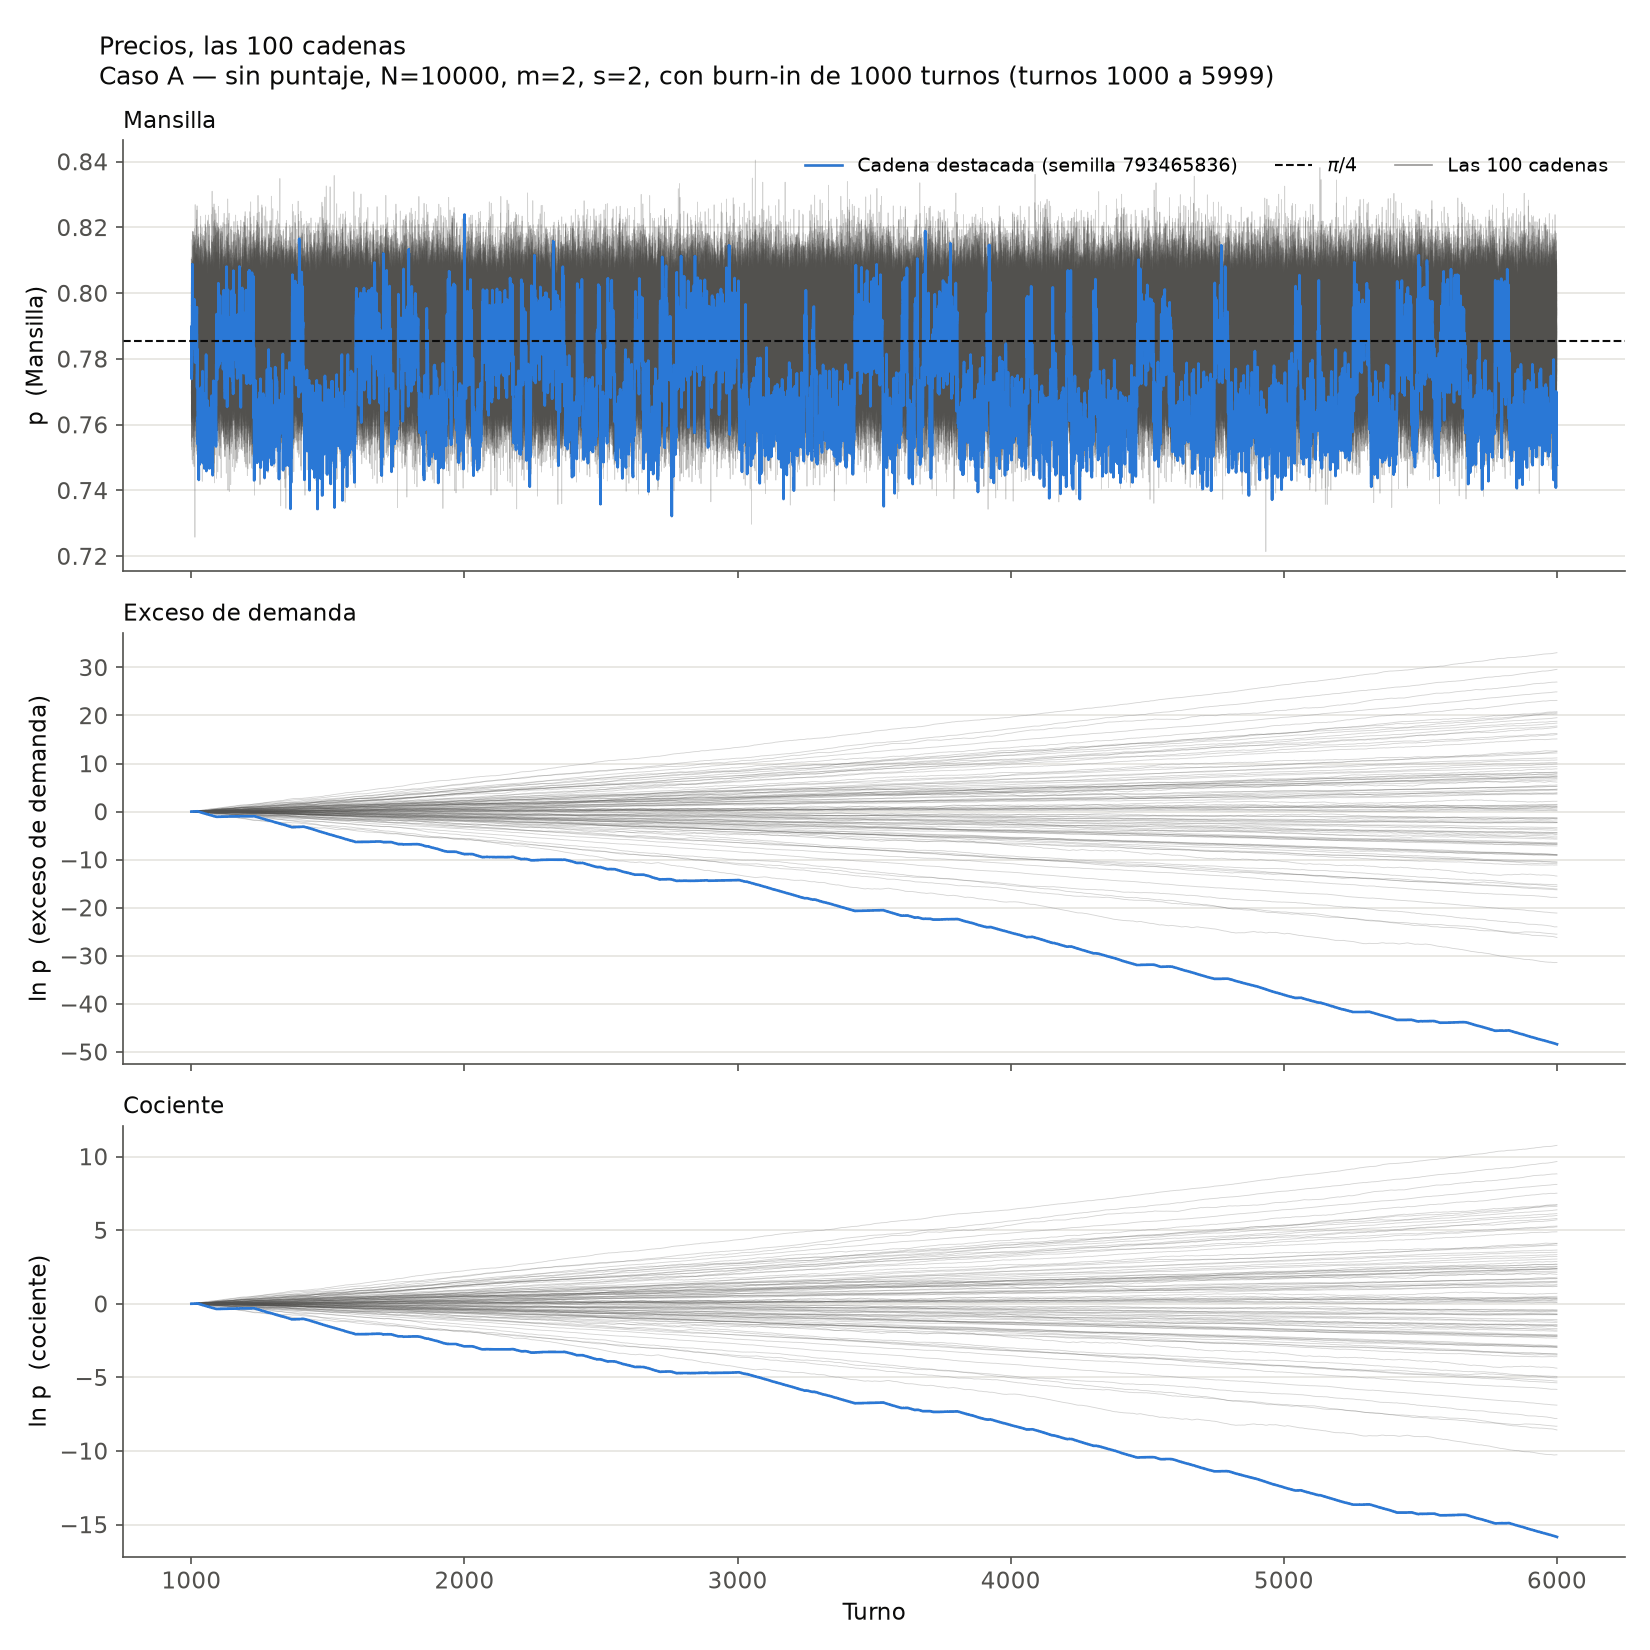
\includegraphics[width=0.49\textwidth]{figuras/Fase9_precios_conjunto_casoA_N10000_m2_s2_sin_puntaje_T6000_regla_nueva_con_burnin1000.png}
\caption{Caso A, $N=10000$: conjunto de precios sin burn-in (izquierda) y con burn-in (derecha).}
\end{figure}

\begin{figure}[H]
\centering
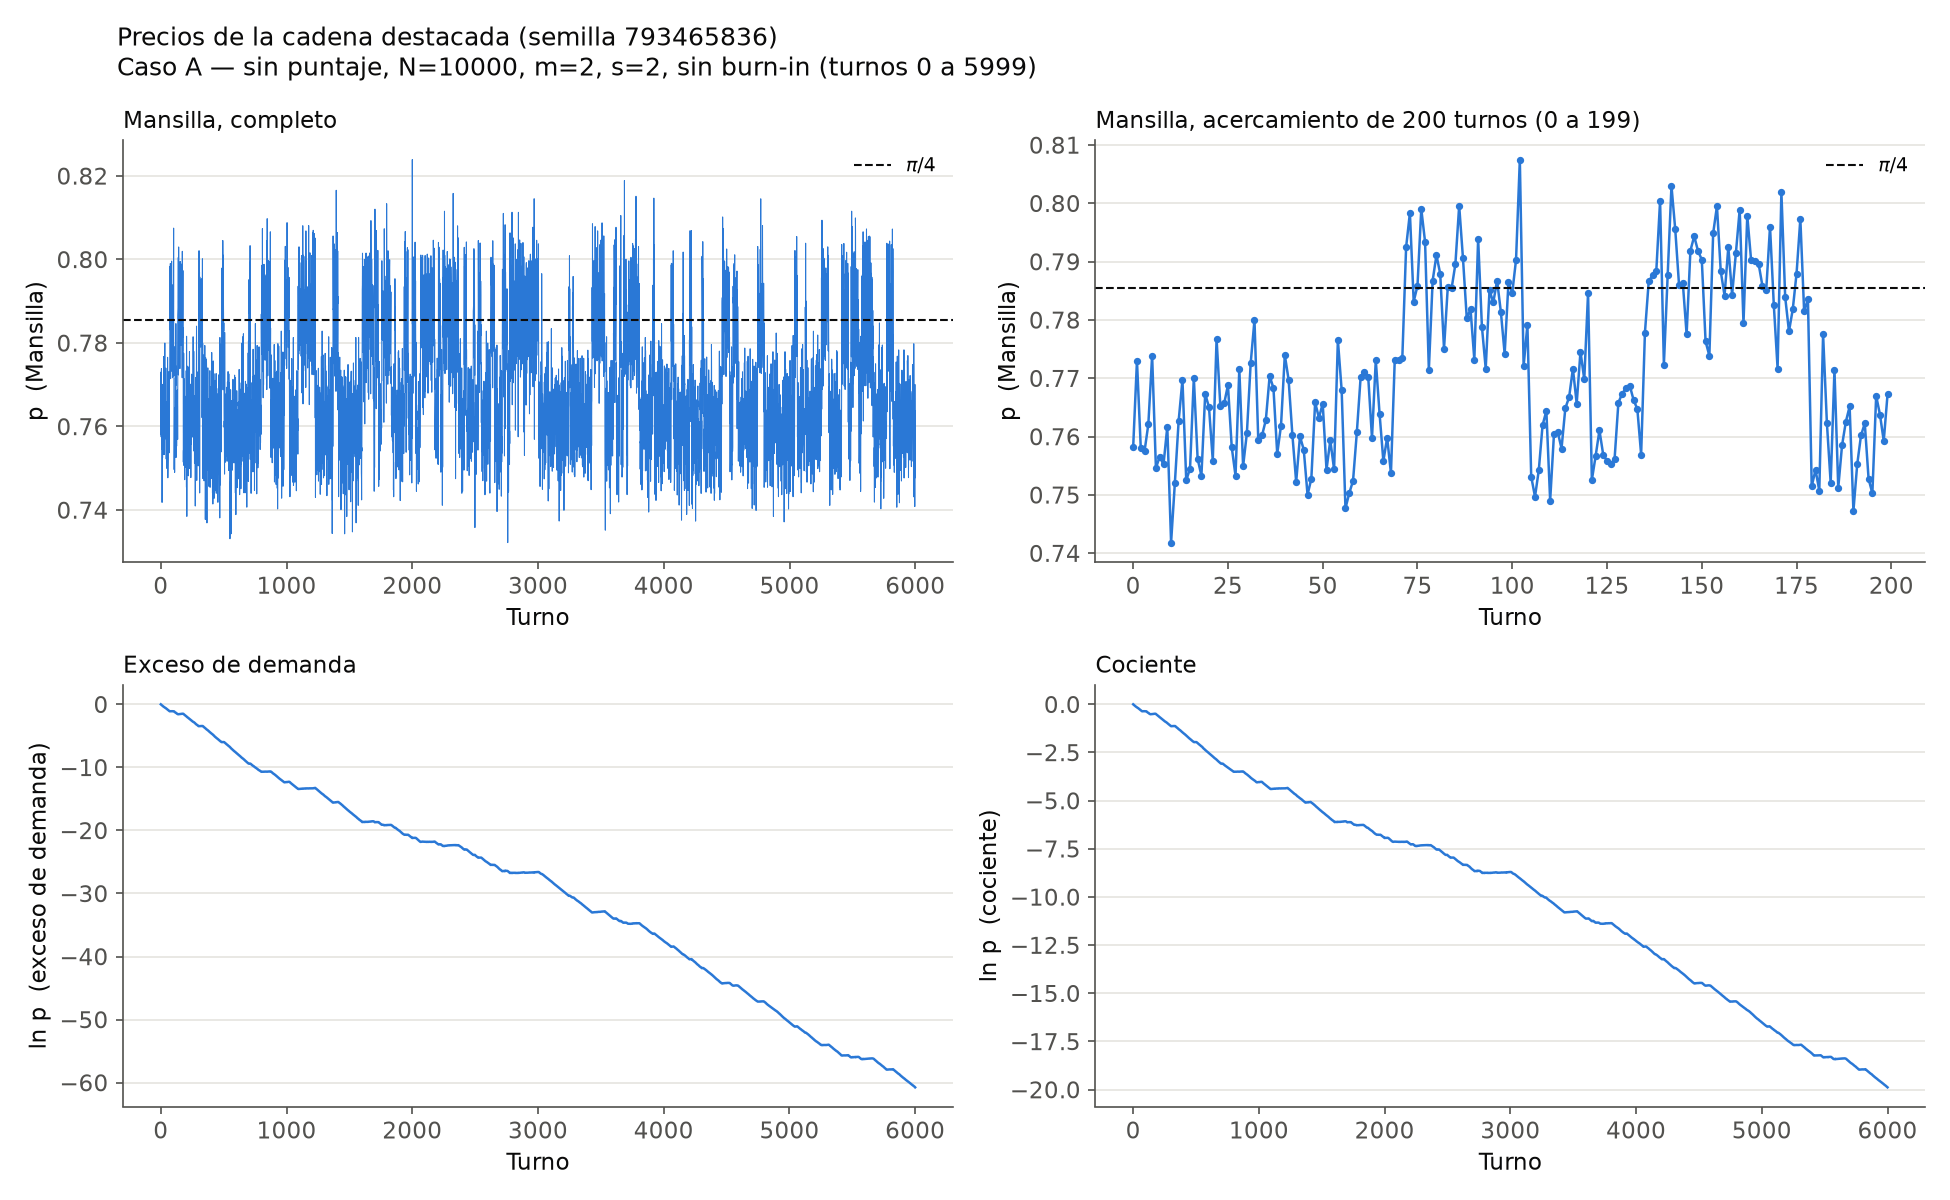
\includegraphics[width=0.49\textwidth]{figuras/Fase9_precios_detalle_casoA_N10000_m2_s2_sin_puntaje_T6000_regla_nueva_sin_burnin.png}\hfill
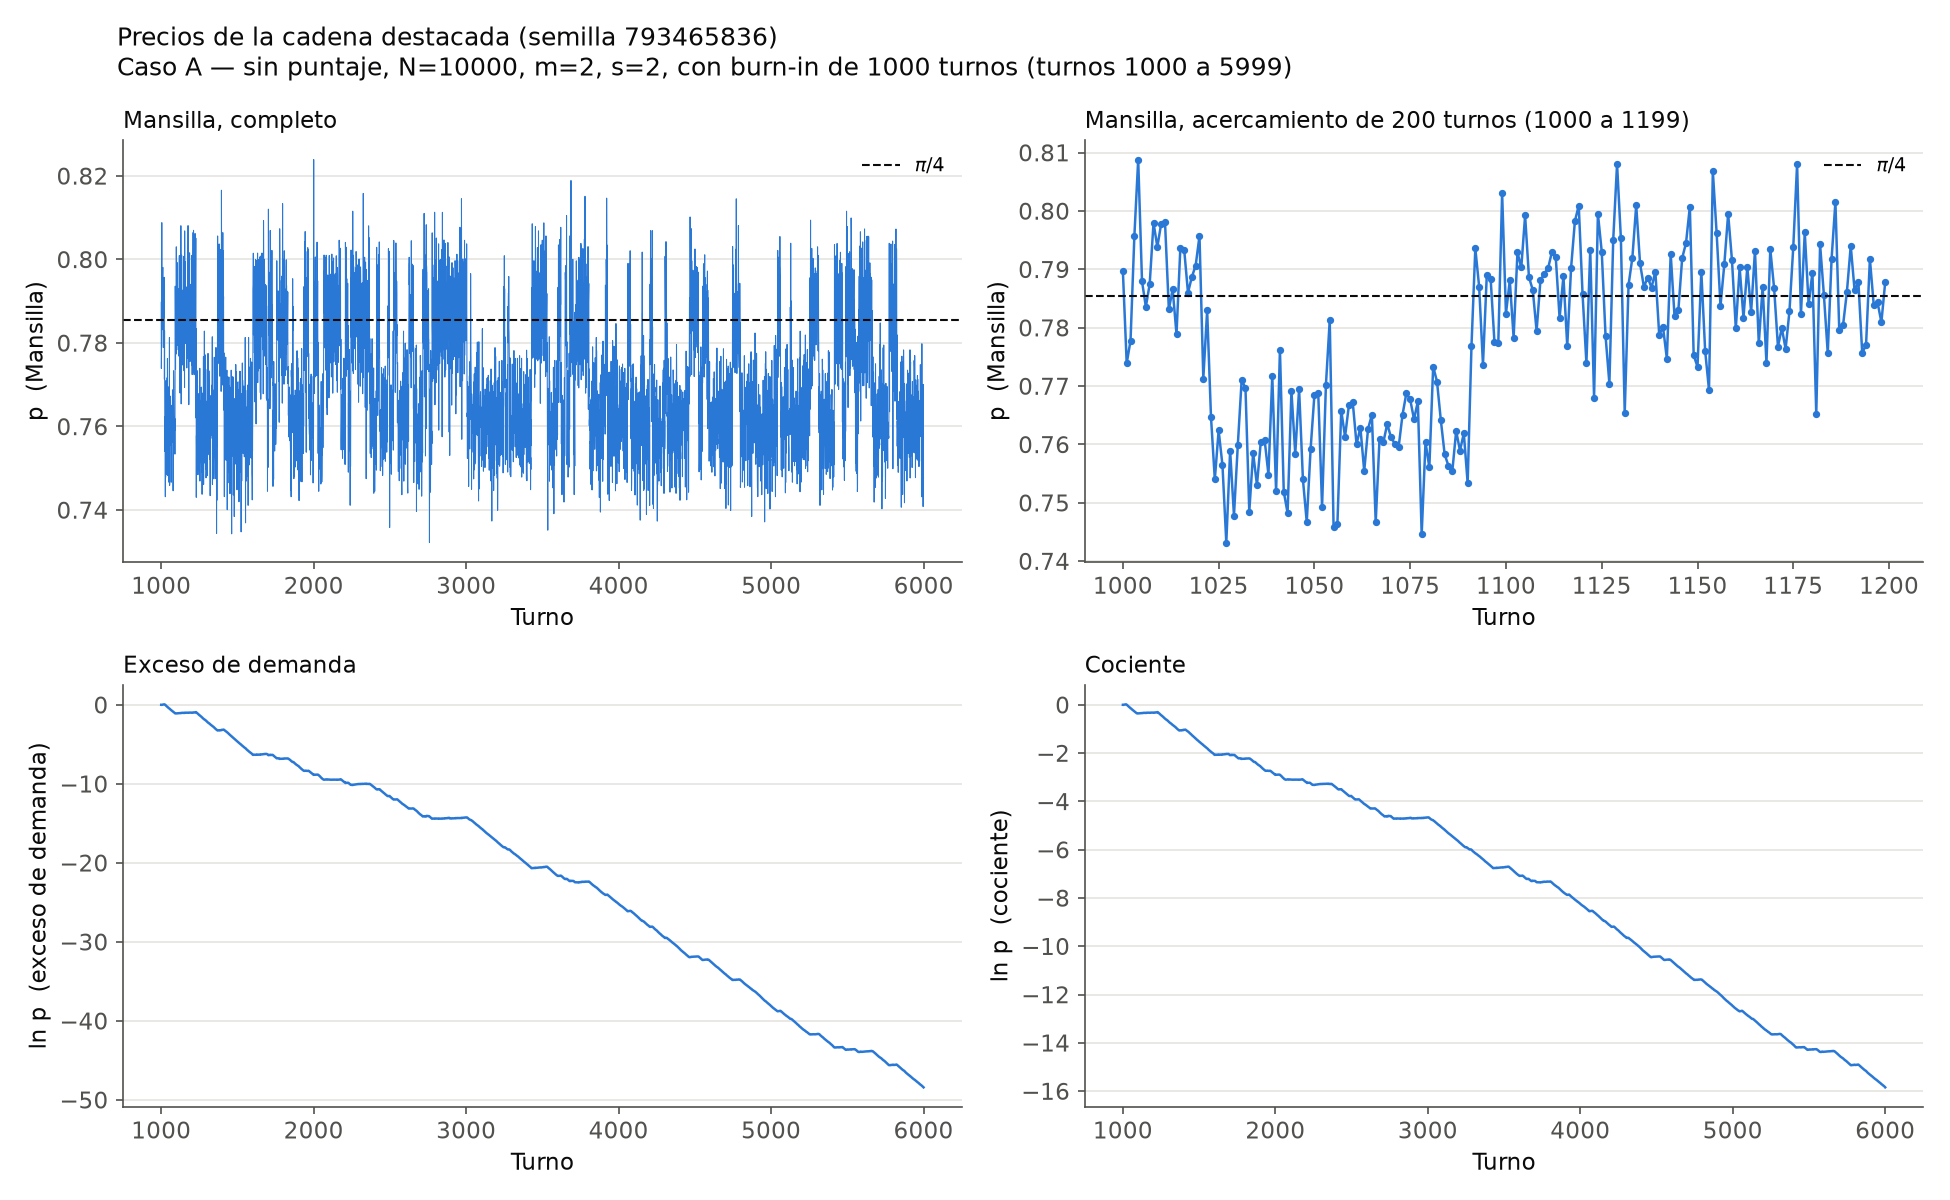
\includegraphics[width=0.49\textwidth]{figuras/Fase9_precios_detalle_casoA_N10000_m2_s2_sin_puntaje_T6000_regla_nueva_con_burnin1000.png}
\caption{Caso A, $N=10000$: detalle de la cadena destacada sin burn-in (izquierda) y con burn-in (derecha).}
\end{figure}

\begin{figure}[H]
\centering
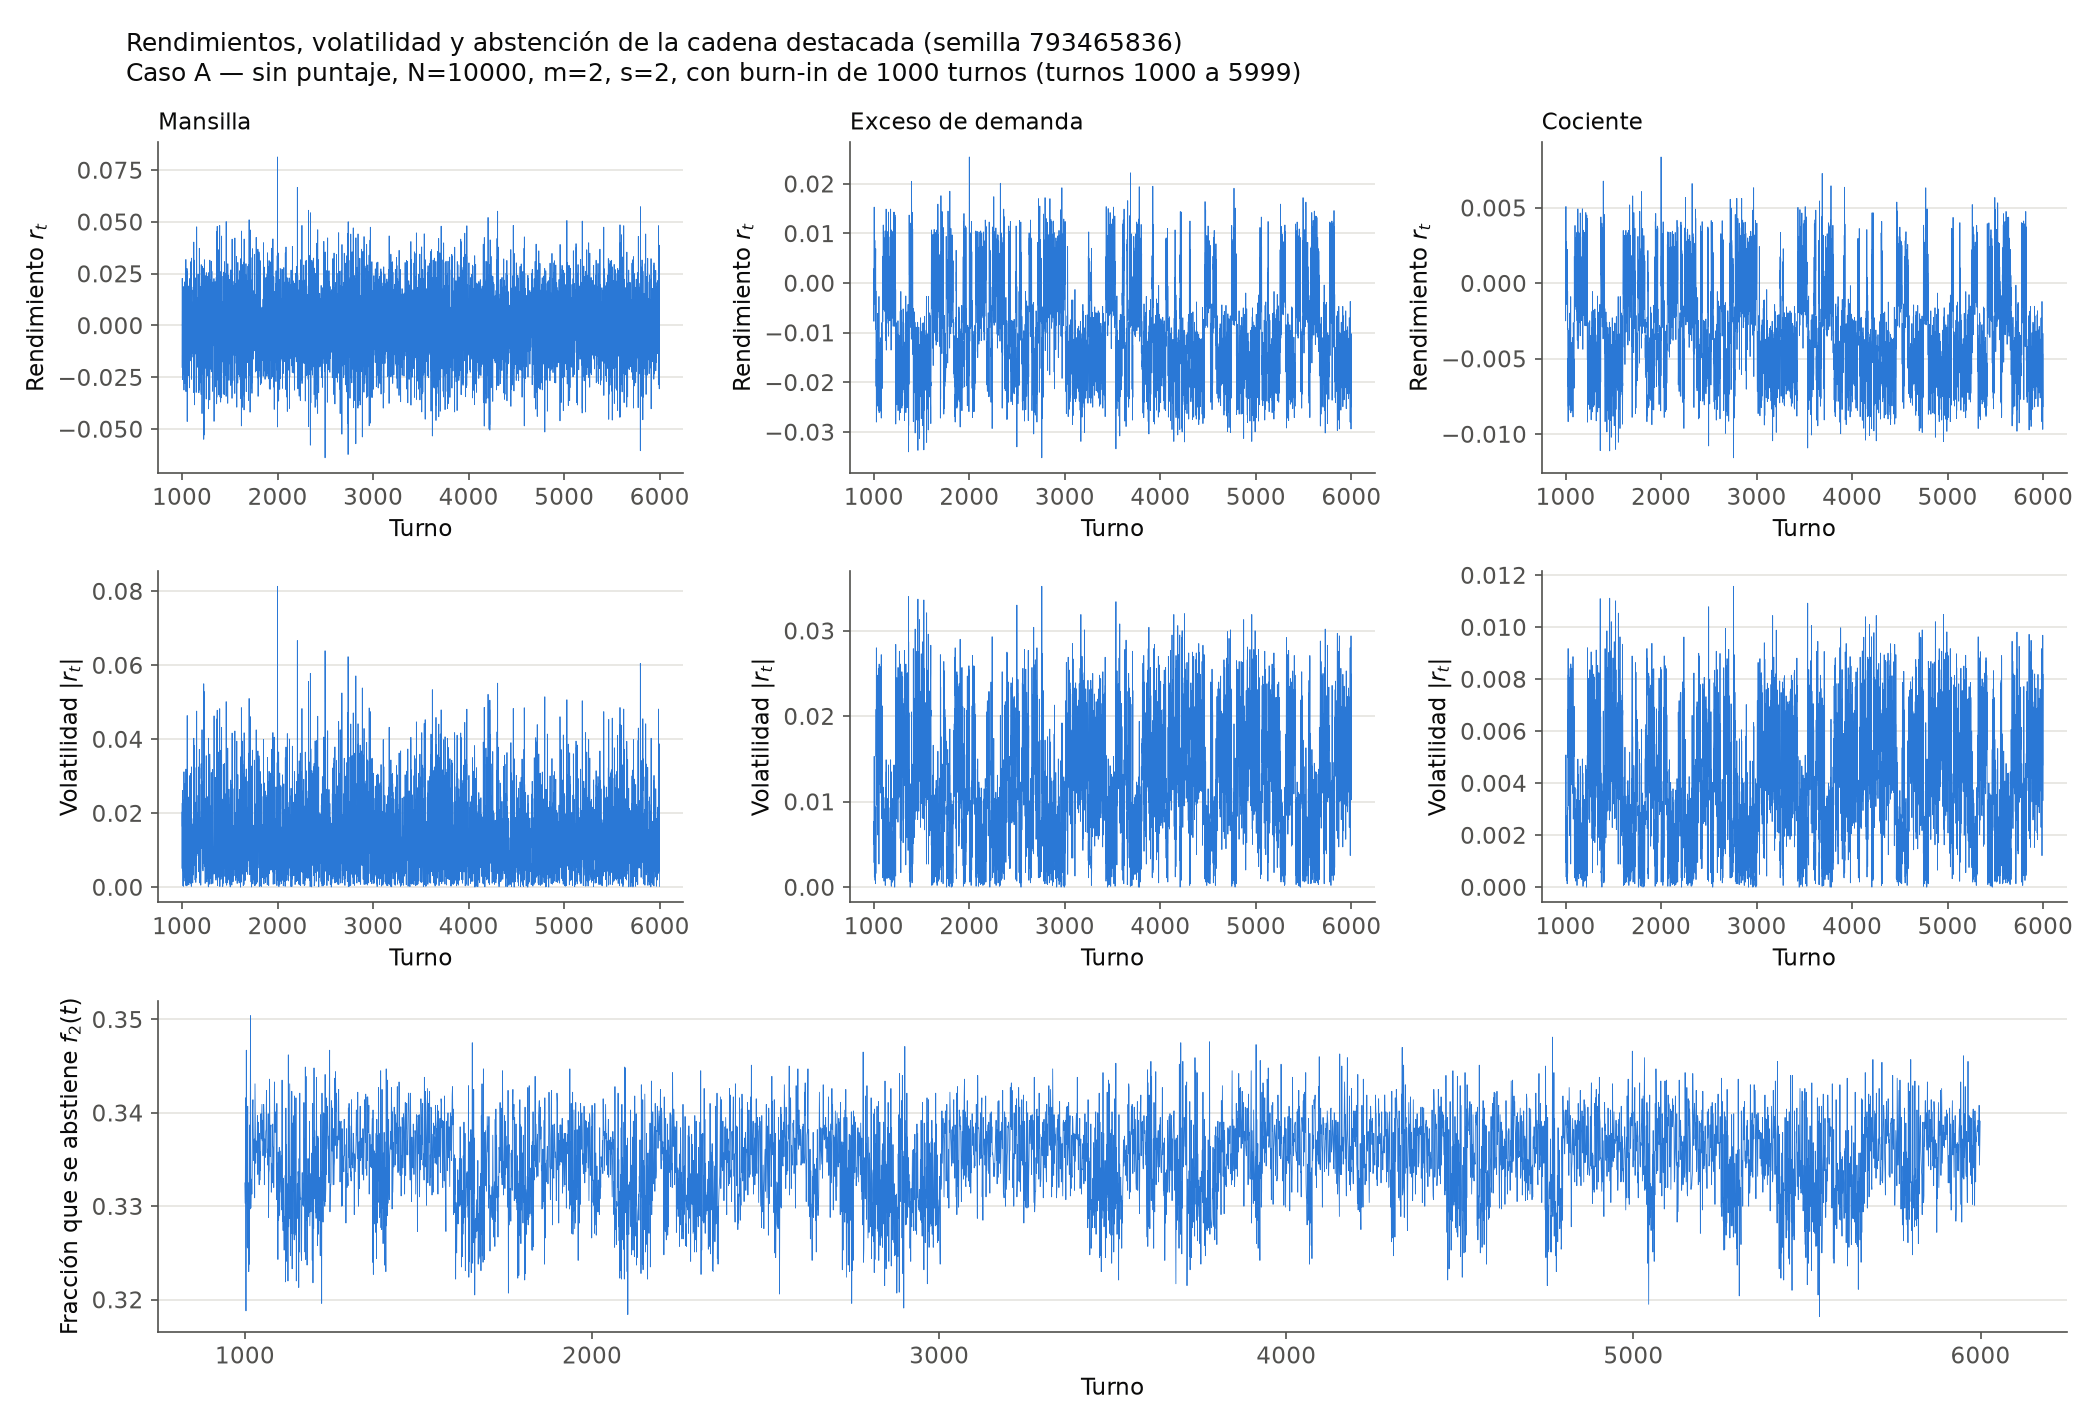
\includegraphics[width=0.85\textwidth]{figuras/Fase9_series_casoA_N10000_m2_s2_sin_puntaje_T6000_regla_nueva_con_burnin1000.png}
\caption{Caso A: rendimientos, volatilidad y fracción que se abstiene de la cadena destacada, con burn-in.}
\end{figure}

\begin{figure}[H]
\centering
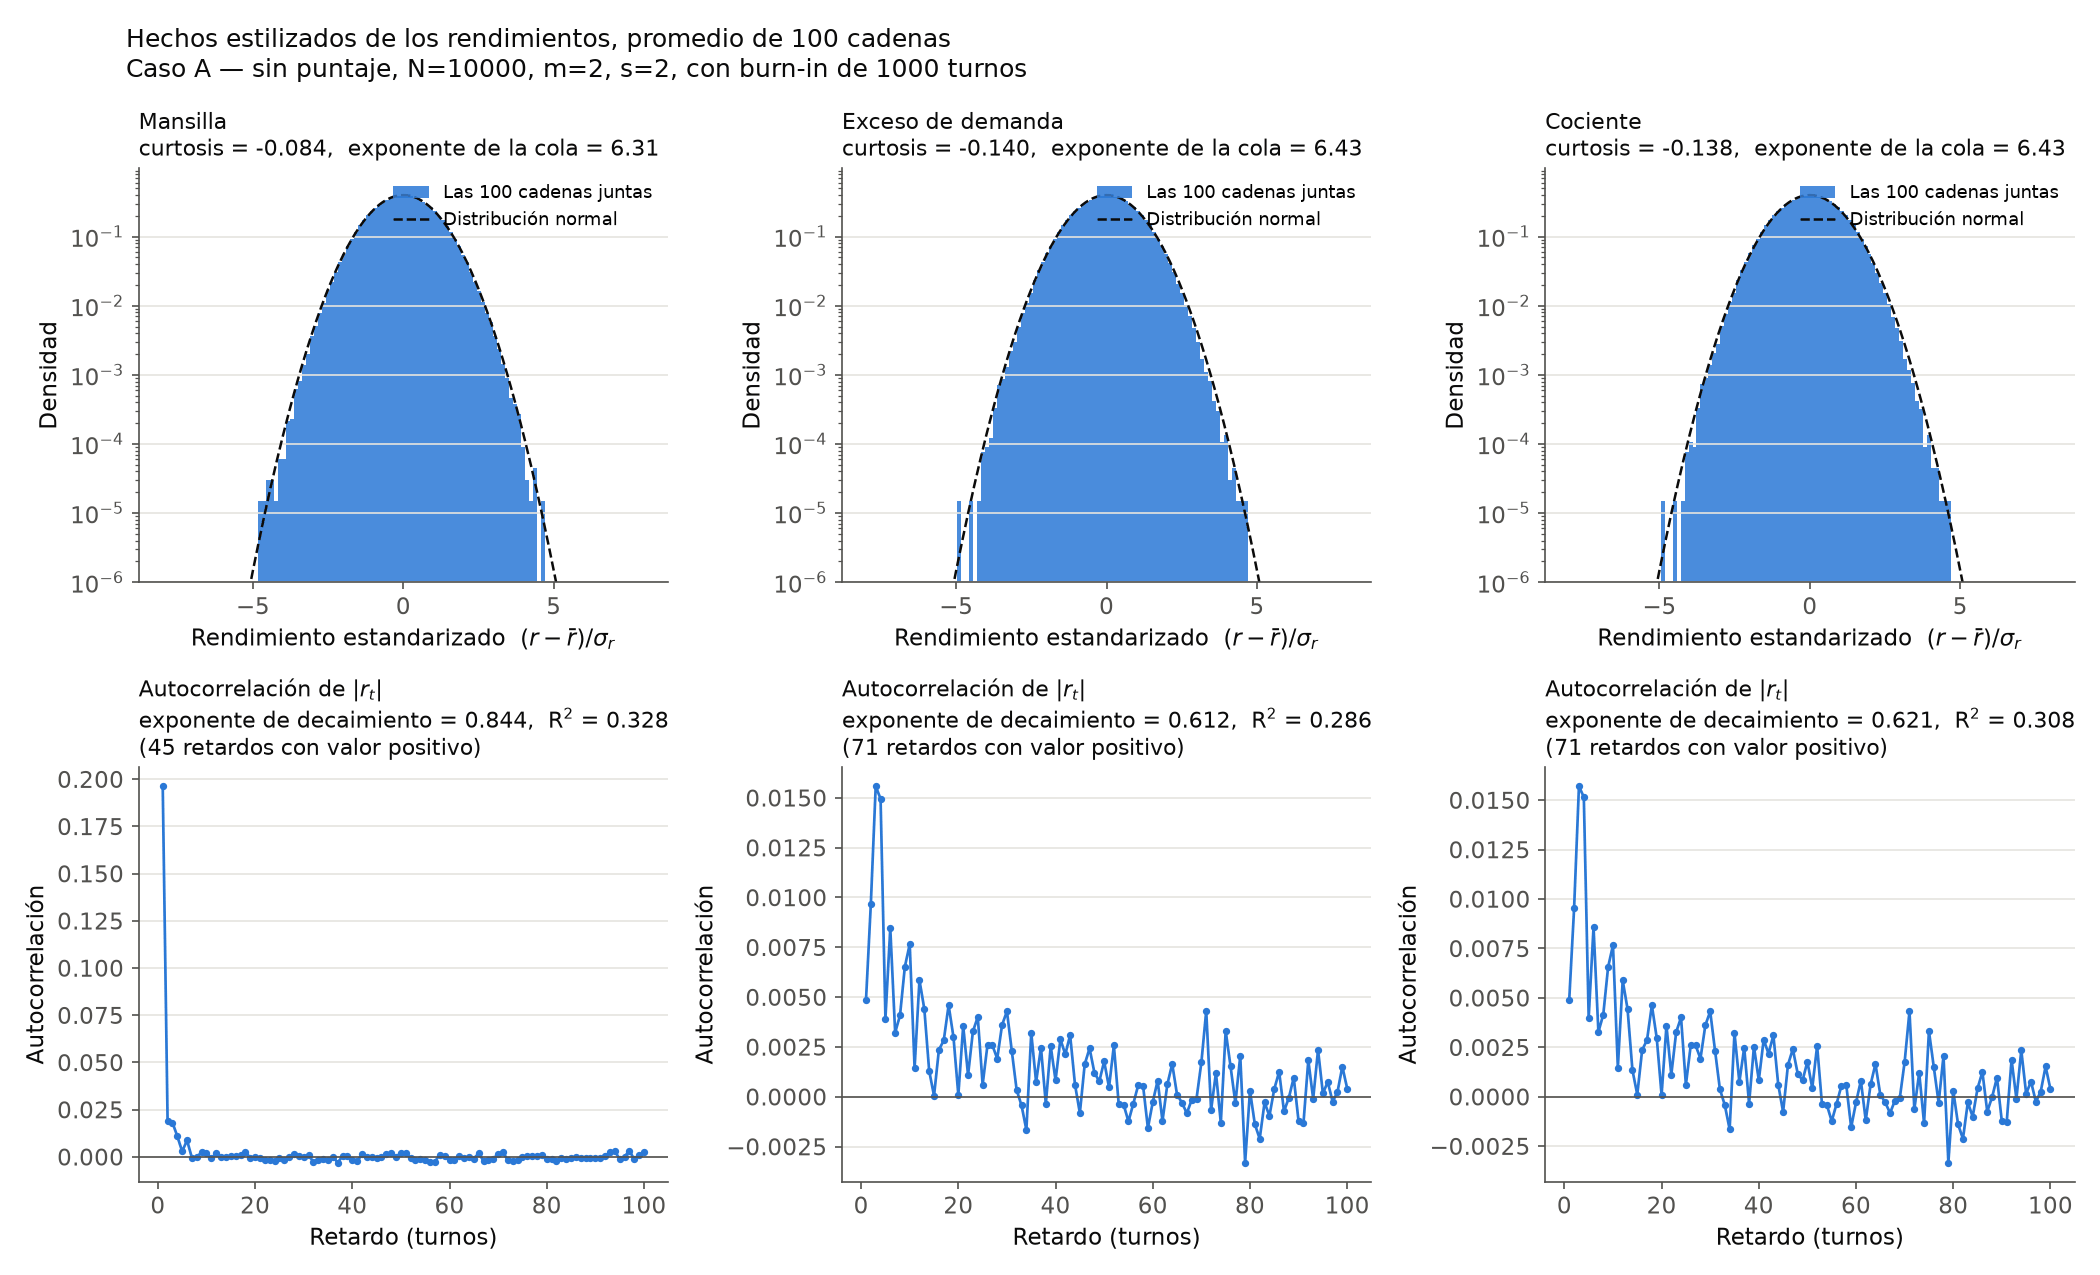
\includegraphics[width=0.85\textwidth]{figuras/Fase9_hechos_estilizados_casoA_N10000_m2_s2_sin_puntaje_T6000_regla_nueva_con_burnin1000.png}
\caption{Caso A: hechos estilizados (distribución de los rendimientos y autocorrelación de $|r|$), con burn-in.}
\end{figure}

\begin{figure}[H]
\centering
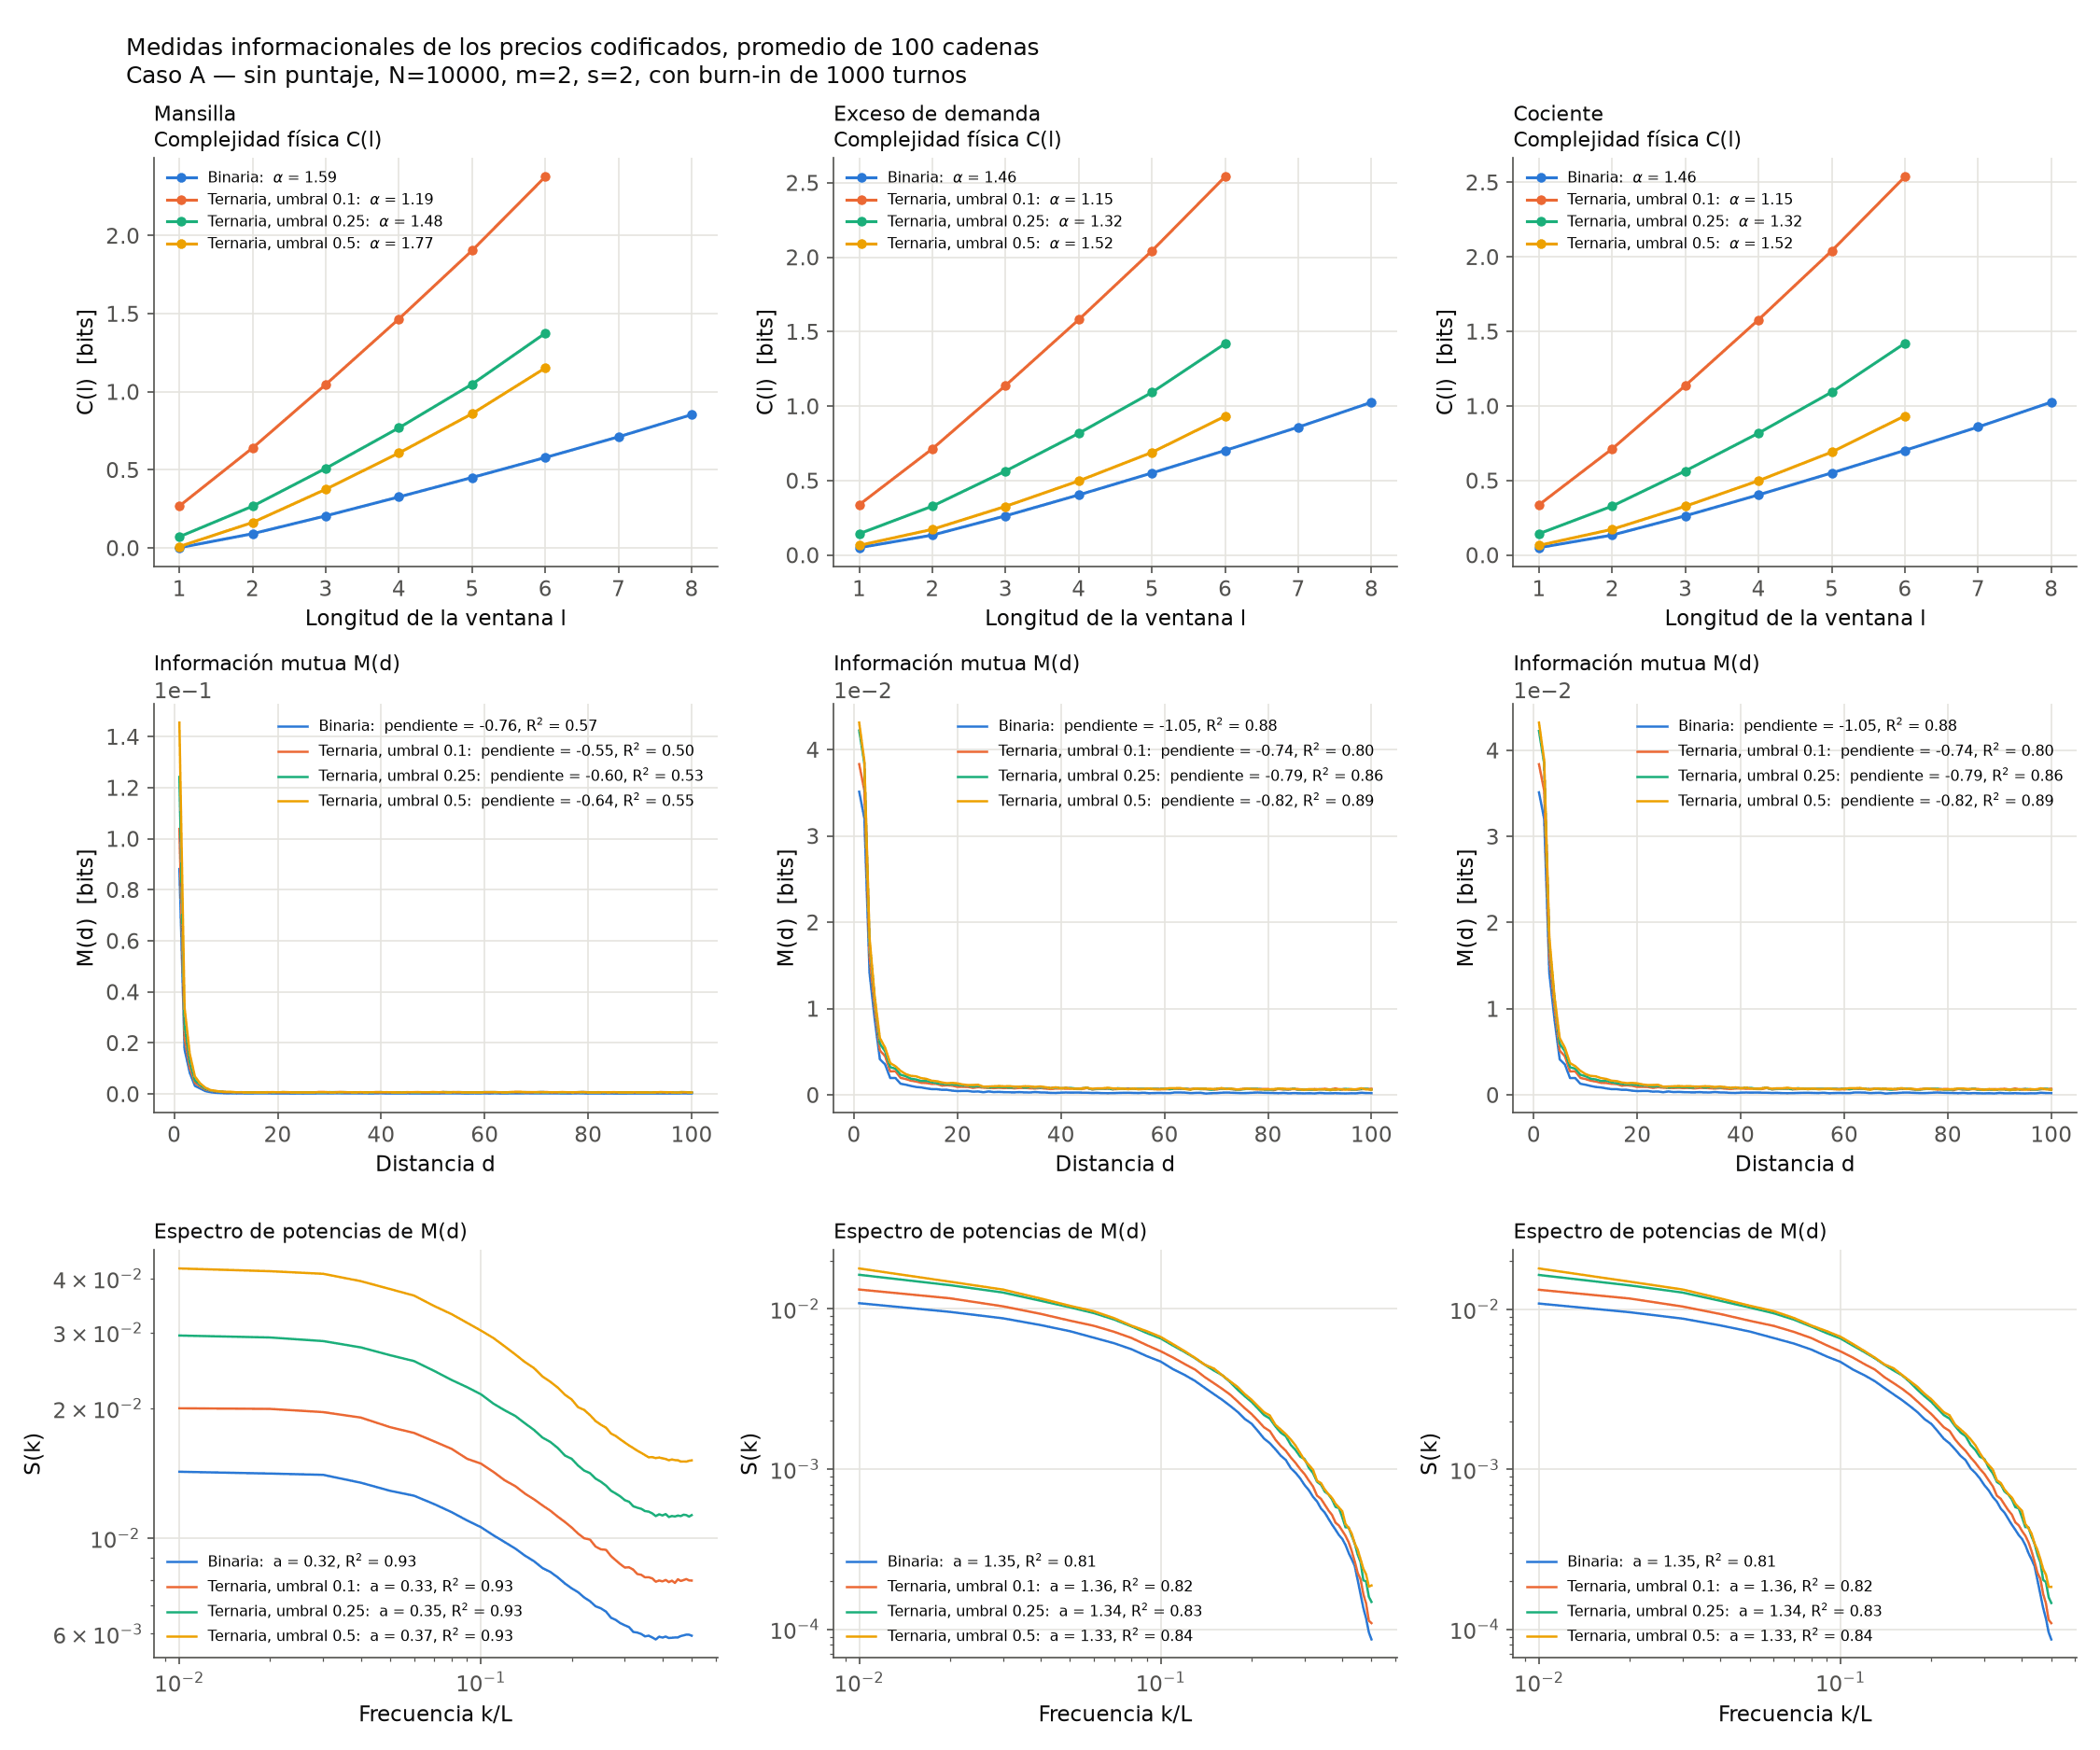
\includegraphics[width=0.85\textwidth]{figuras/Fase9_medidas_informacionales_casoA_N10000_m2_s2_sin_puntaje_T6000_regla_nueva_con_burnin1000.png}
\caption{Caso A: medidas informacionales de los precios codificados, con burn-in.}
\end{figure}

\clearpage
\subsection{Caso B: $m=2$, con puntaje}
\begin{figure}[H]
\centering
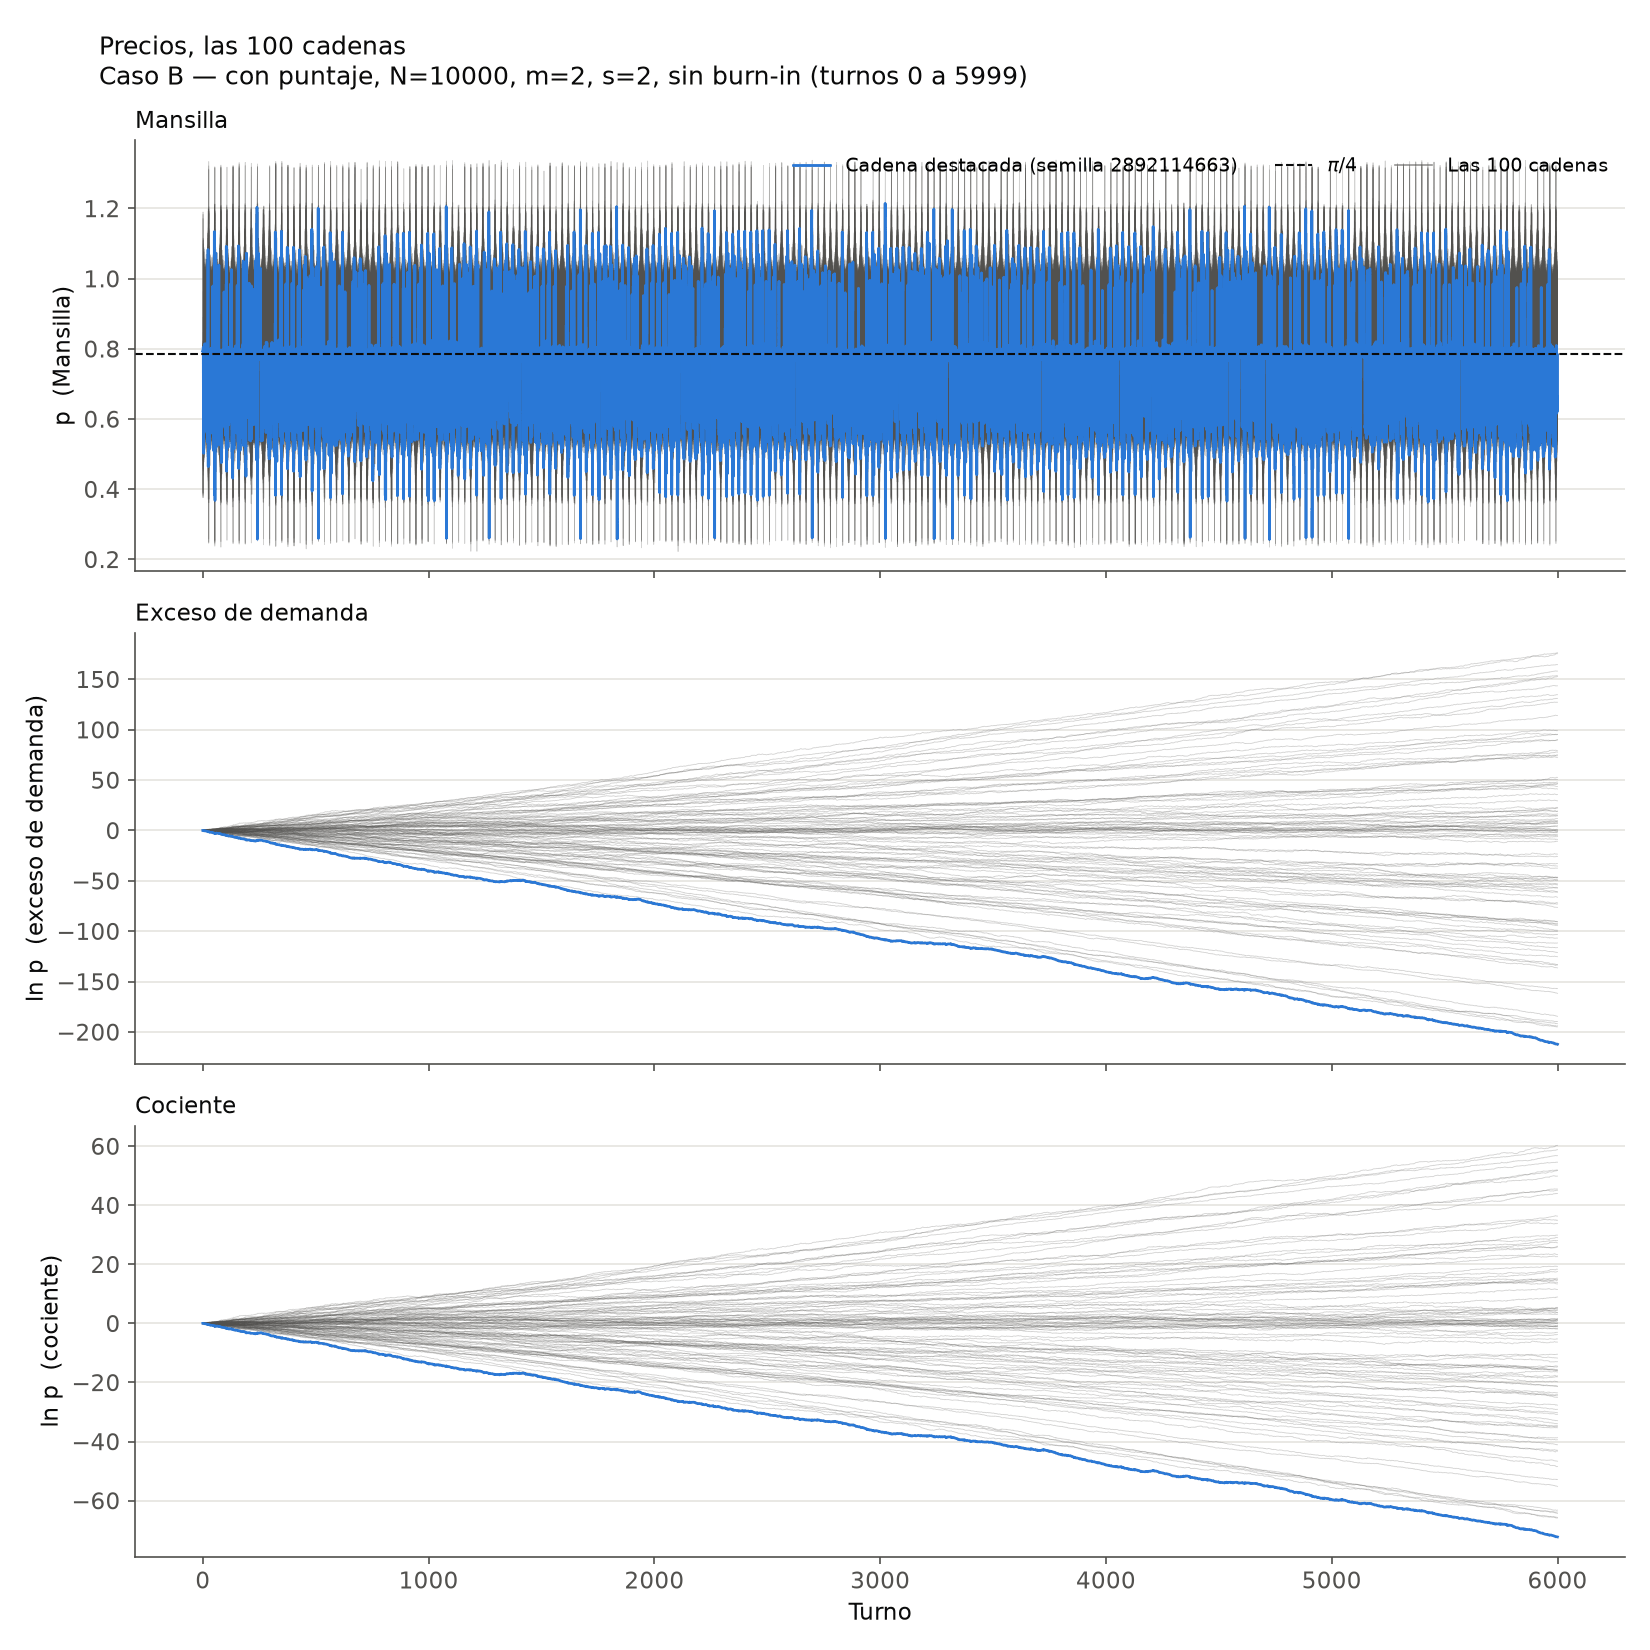
\includegraphics[width=0.49\textwidth]{figuras/Fase9_precios_conjunto_casoB_N10000_m2_s2_con_puntaje_T6000_regla_nueva_sin_burnin.png}\hfill
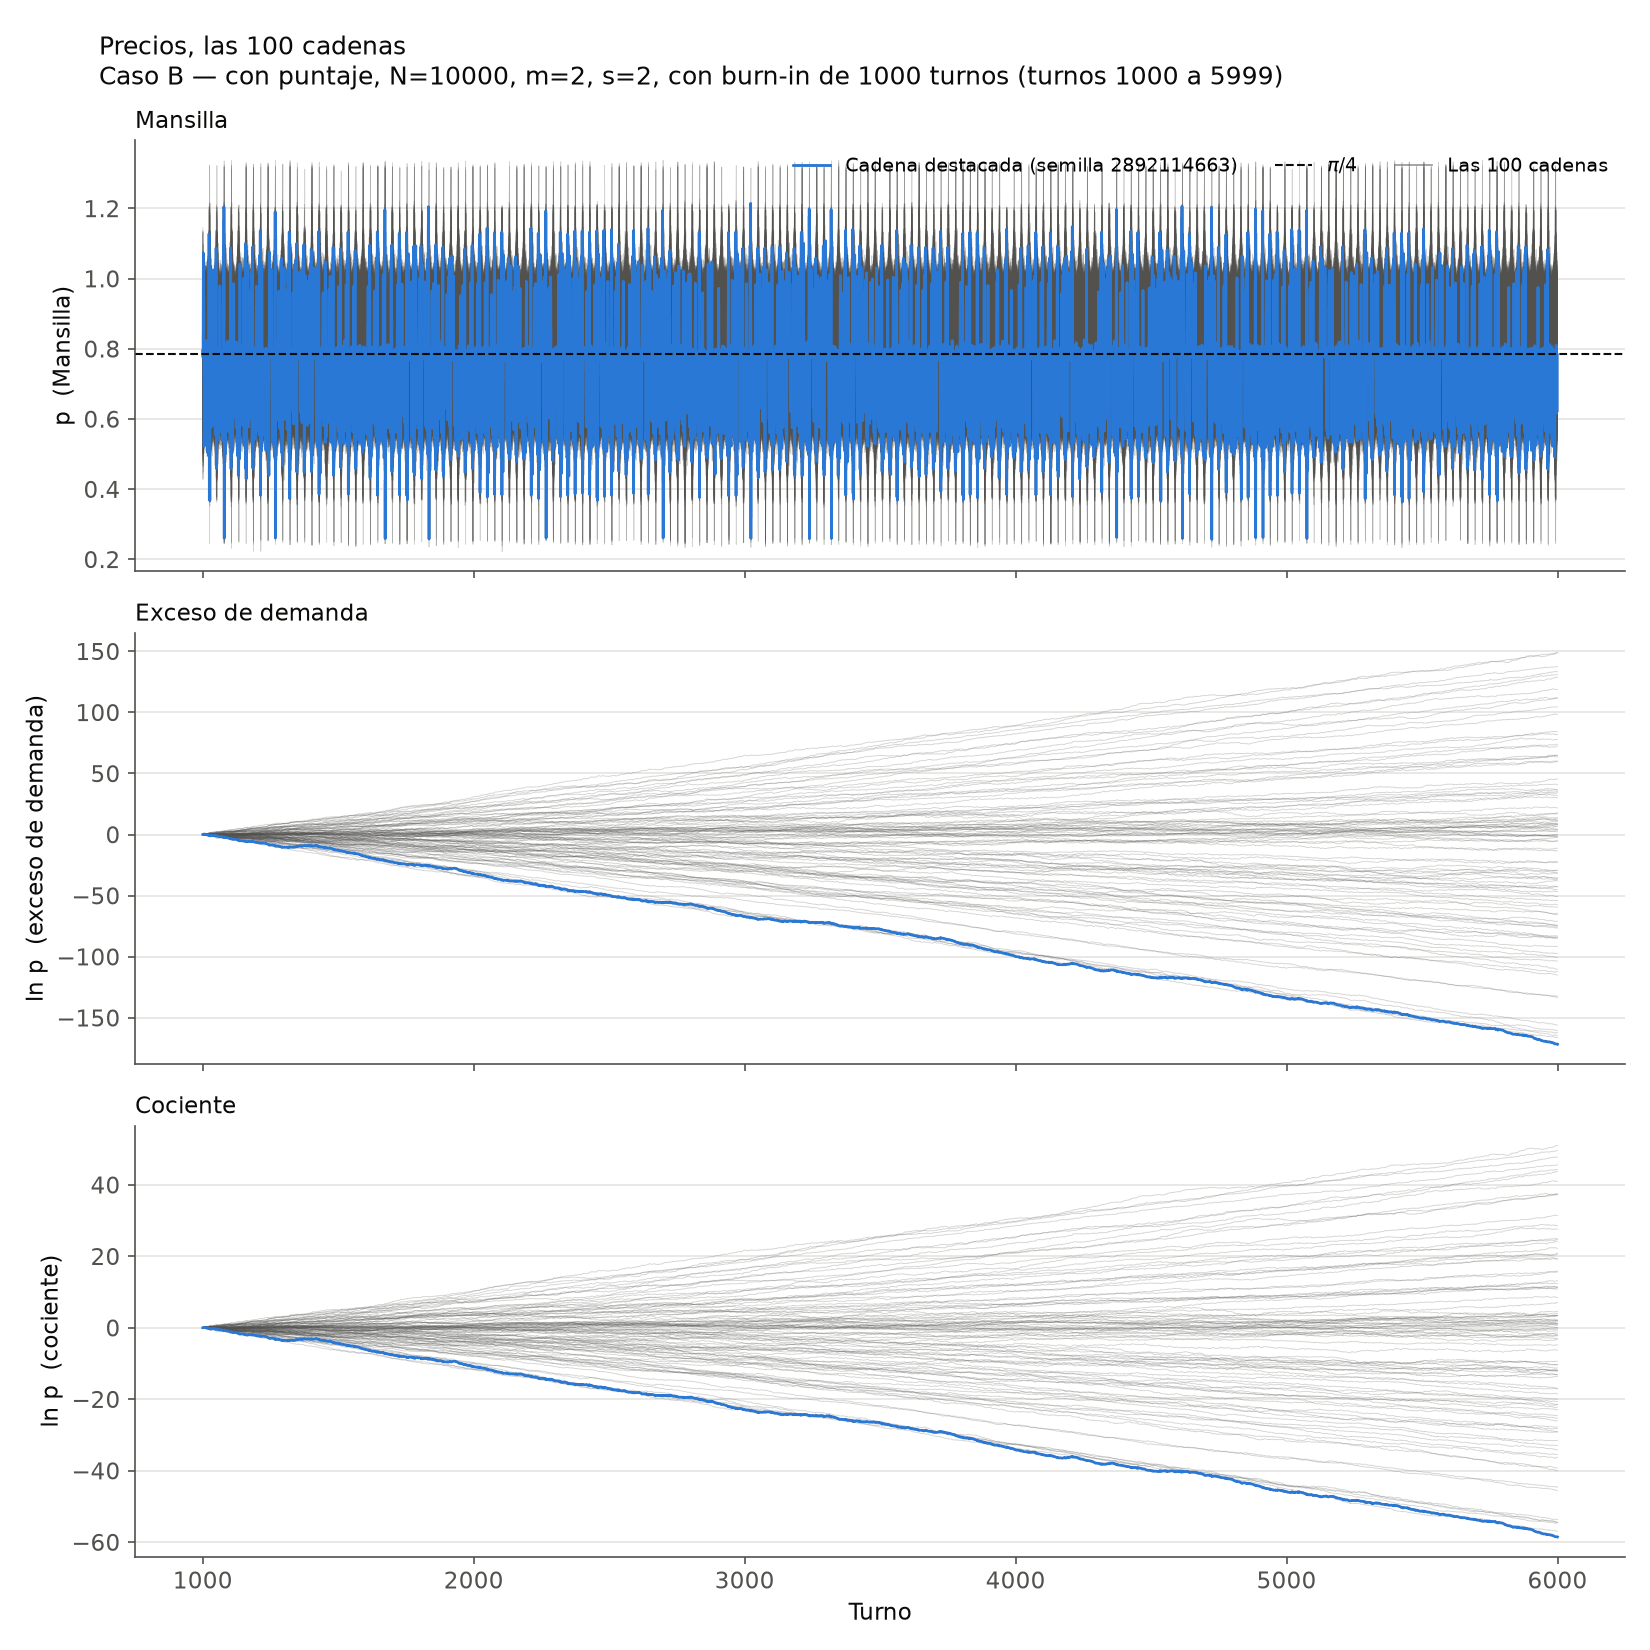
\includegraphics[width=0.49\textwidth]{figuras/Fase9_precios_conjunto_casoB_N10000_m2_s2_con_puntaje_T6000_regla_nueva_con_burnin1000.png}
\caption{Caso B, $N=10000$: conjunto de precios sin burn-in (izquierda) y con burn-in (derecha).}
\end{figure}

\begin{figure}[H]
\centering
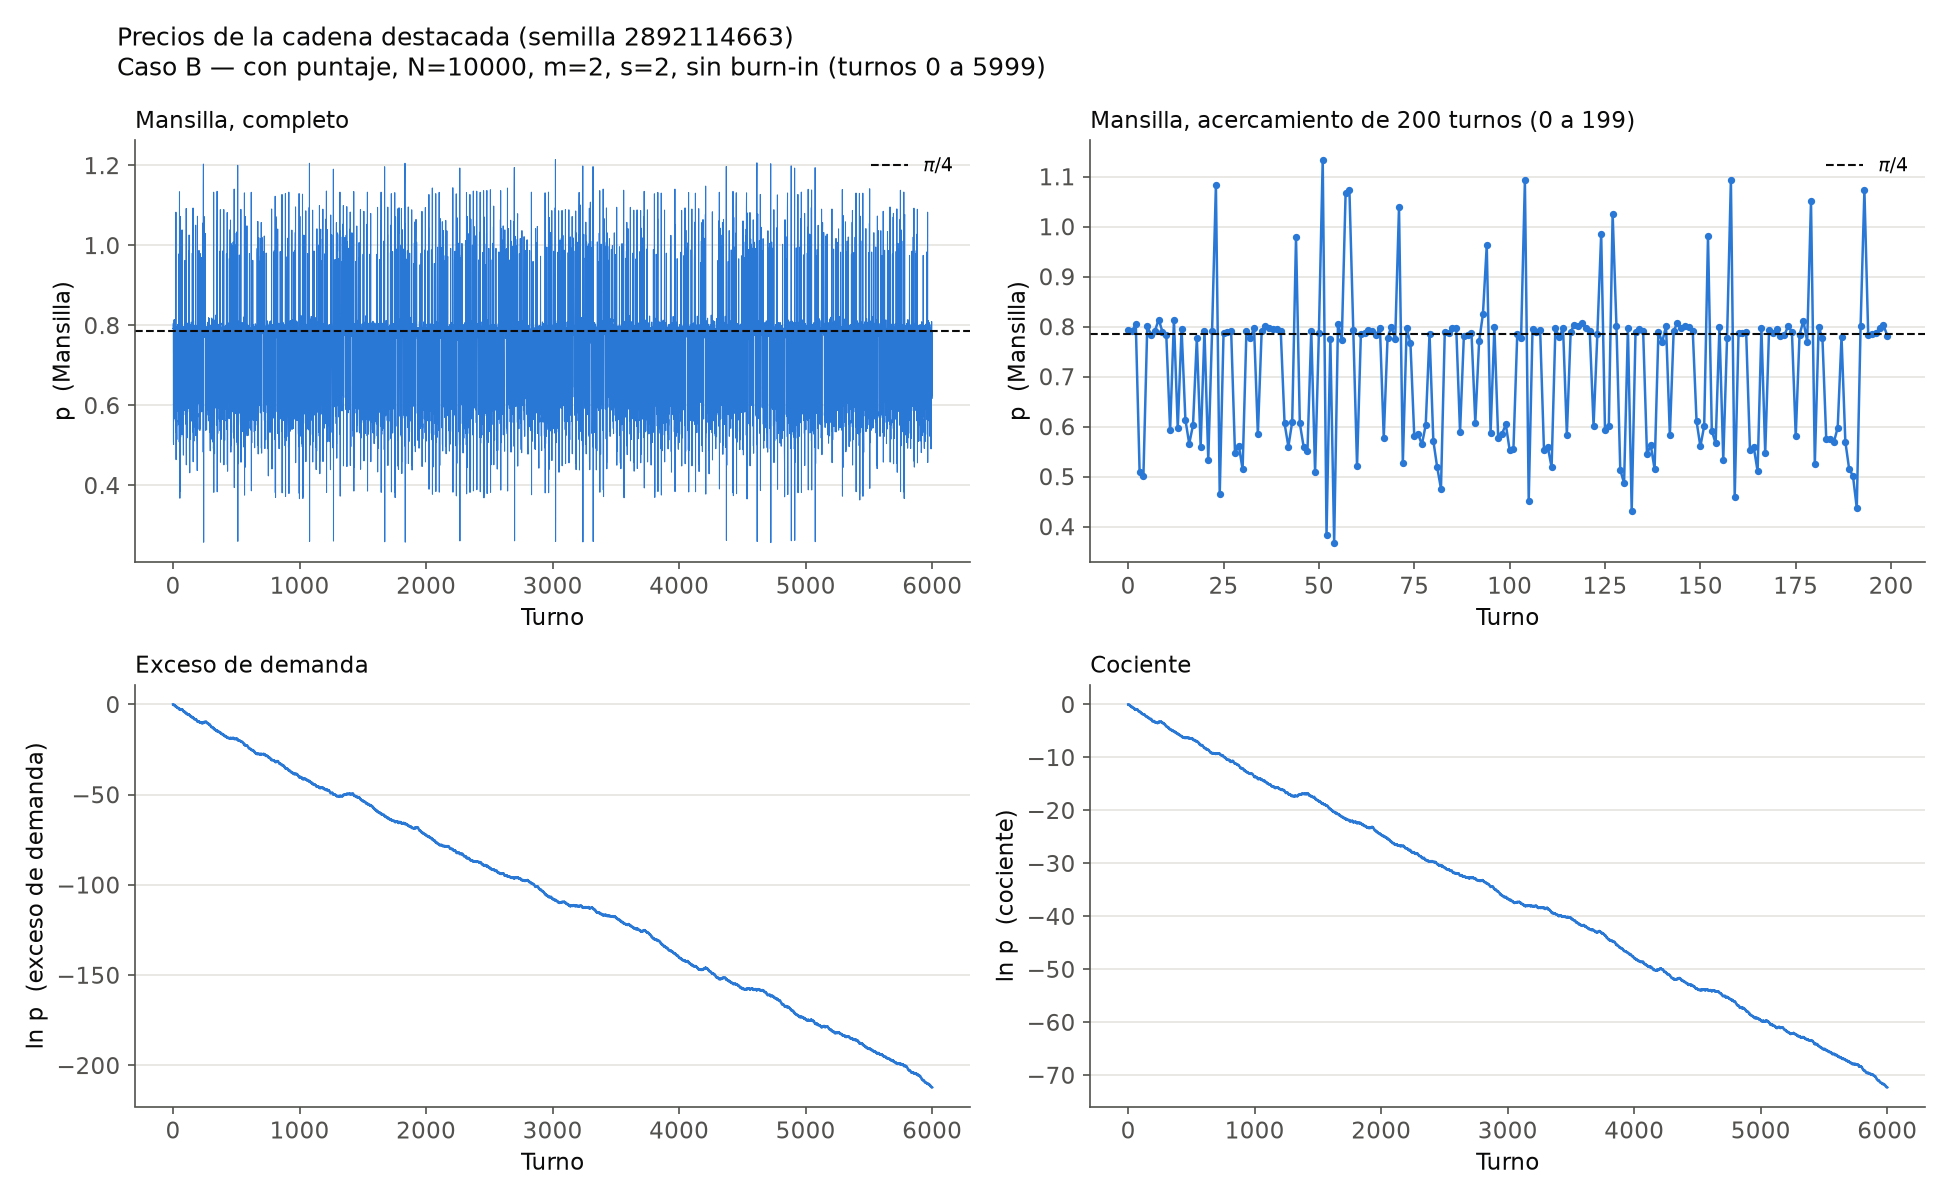
\includegraphics[width=0.49\textwidth]{figuras/Fase9_precios_detalle_casoB_N10000_m2_s2_con_puntaje_T6000_regla_nueva_sin_burnin.png}\hfill
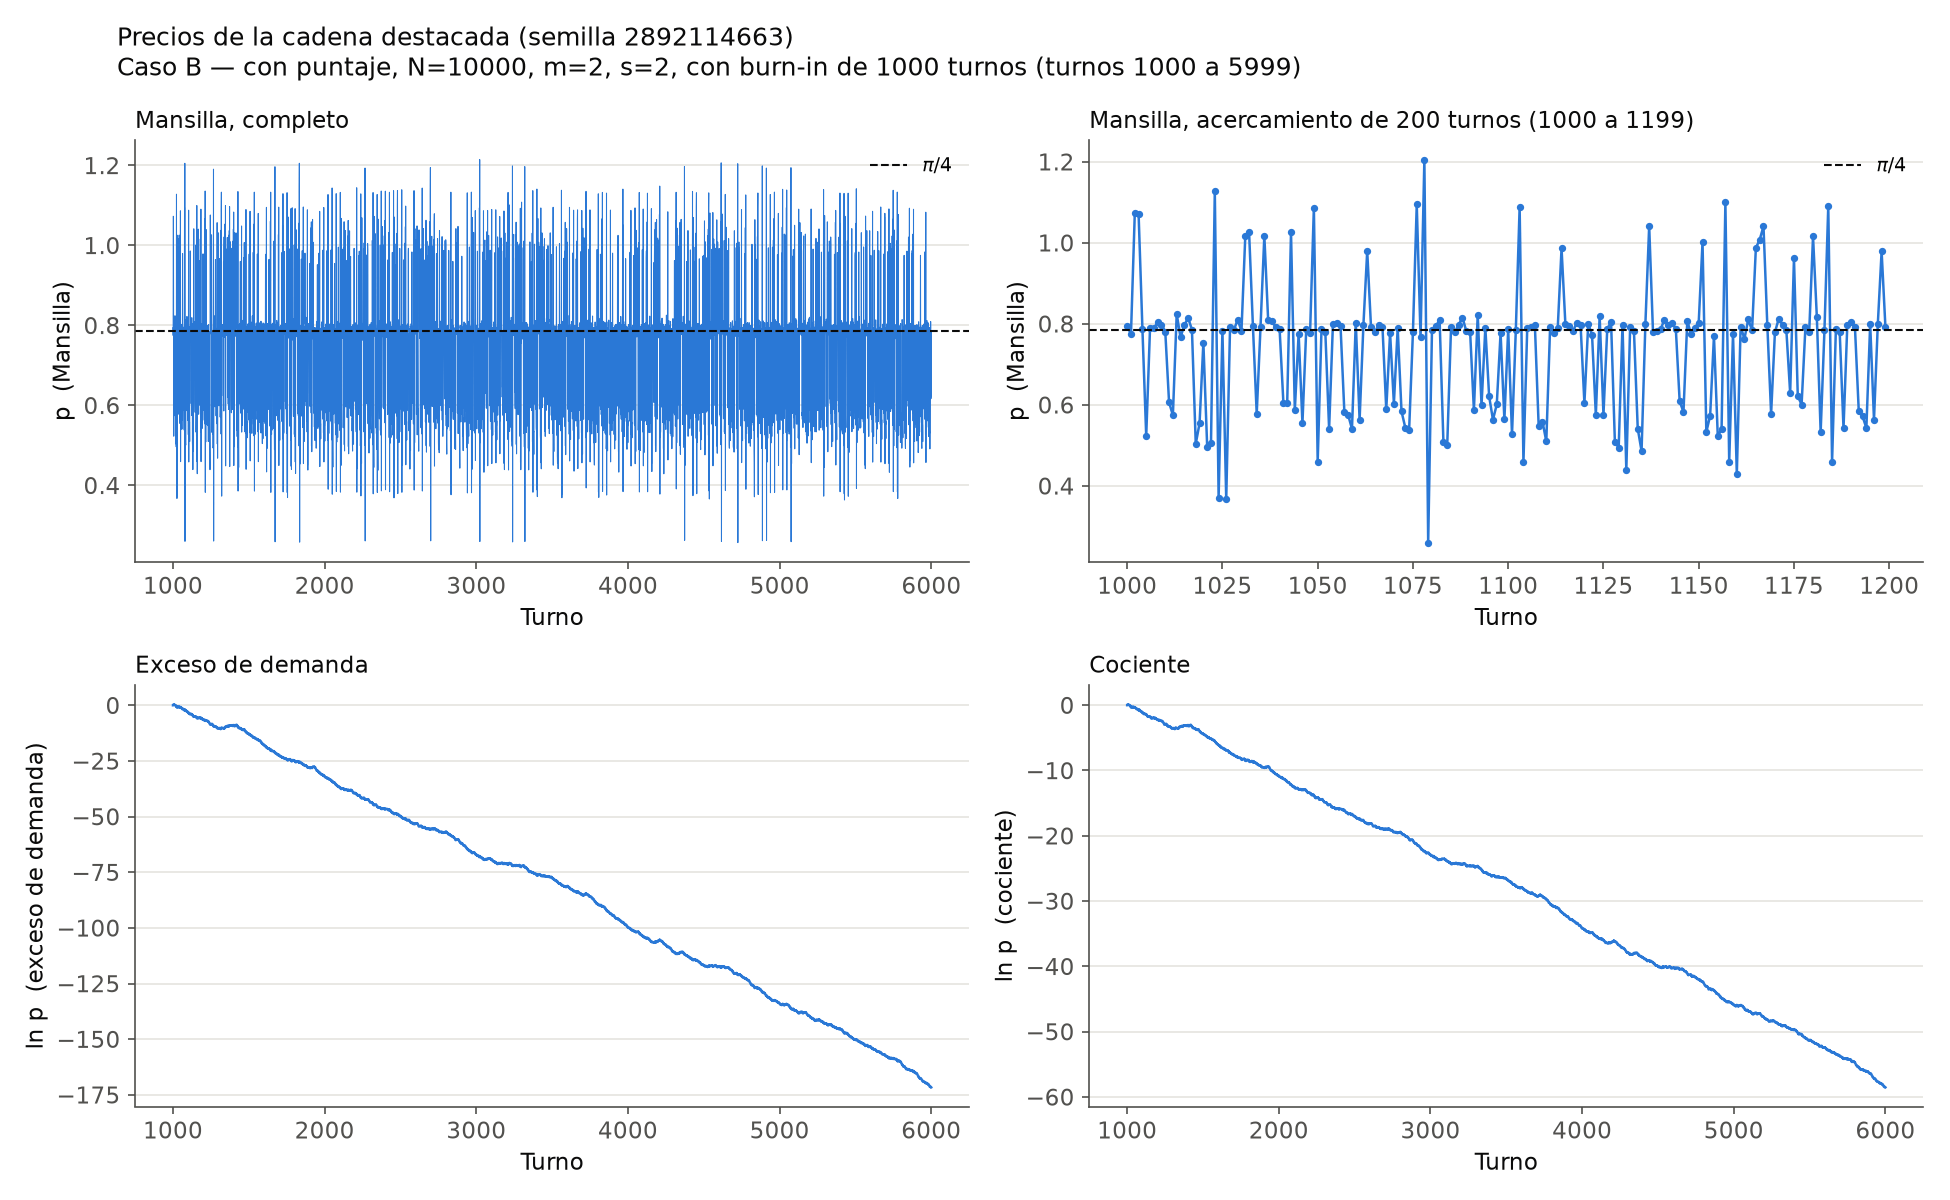
\includegraphics[width=0.49\textwidth]{figuras/Fase9_precios_detalle_casoB_N10000_m2_s2_con_puntaje_T6000_regla_nueva_con_burnin1000.png}
\caption{Caso B, $N=10000$: detalle de la cadena destacada sin burn-in (izquierda) y con burn-in (derecha).}
\end{figure}

\begin{figure}[H]
\centering
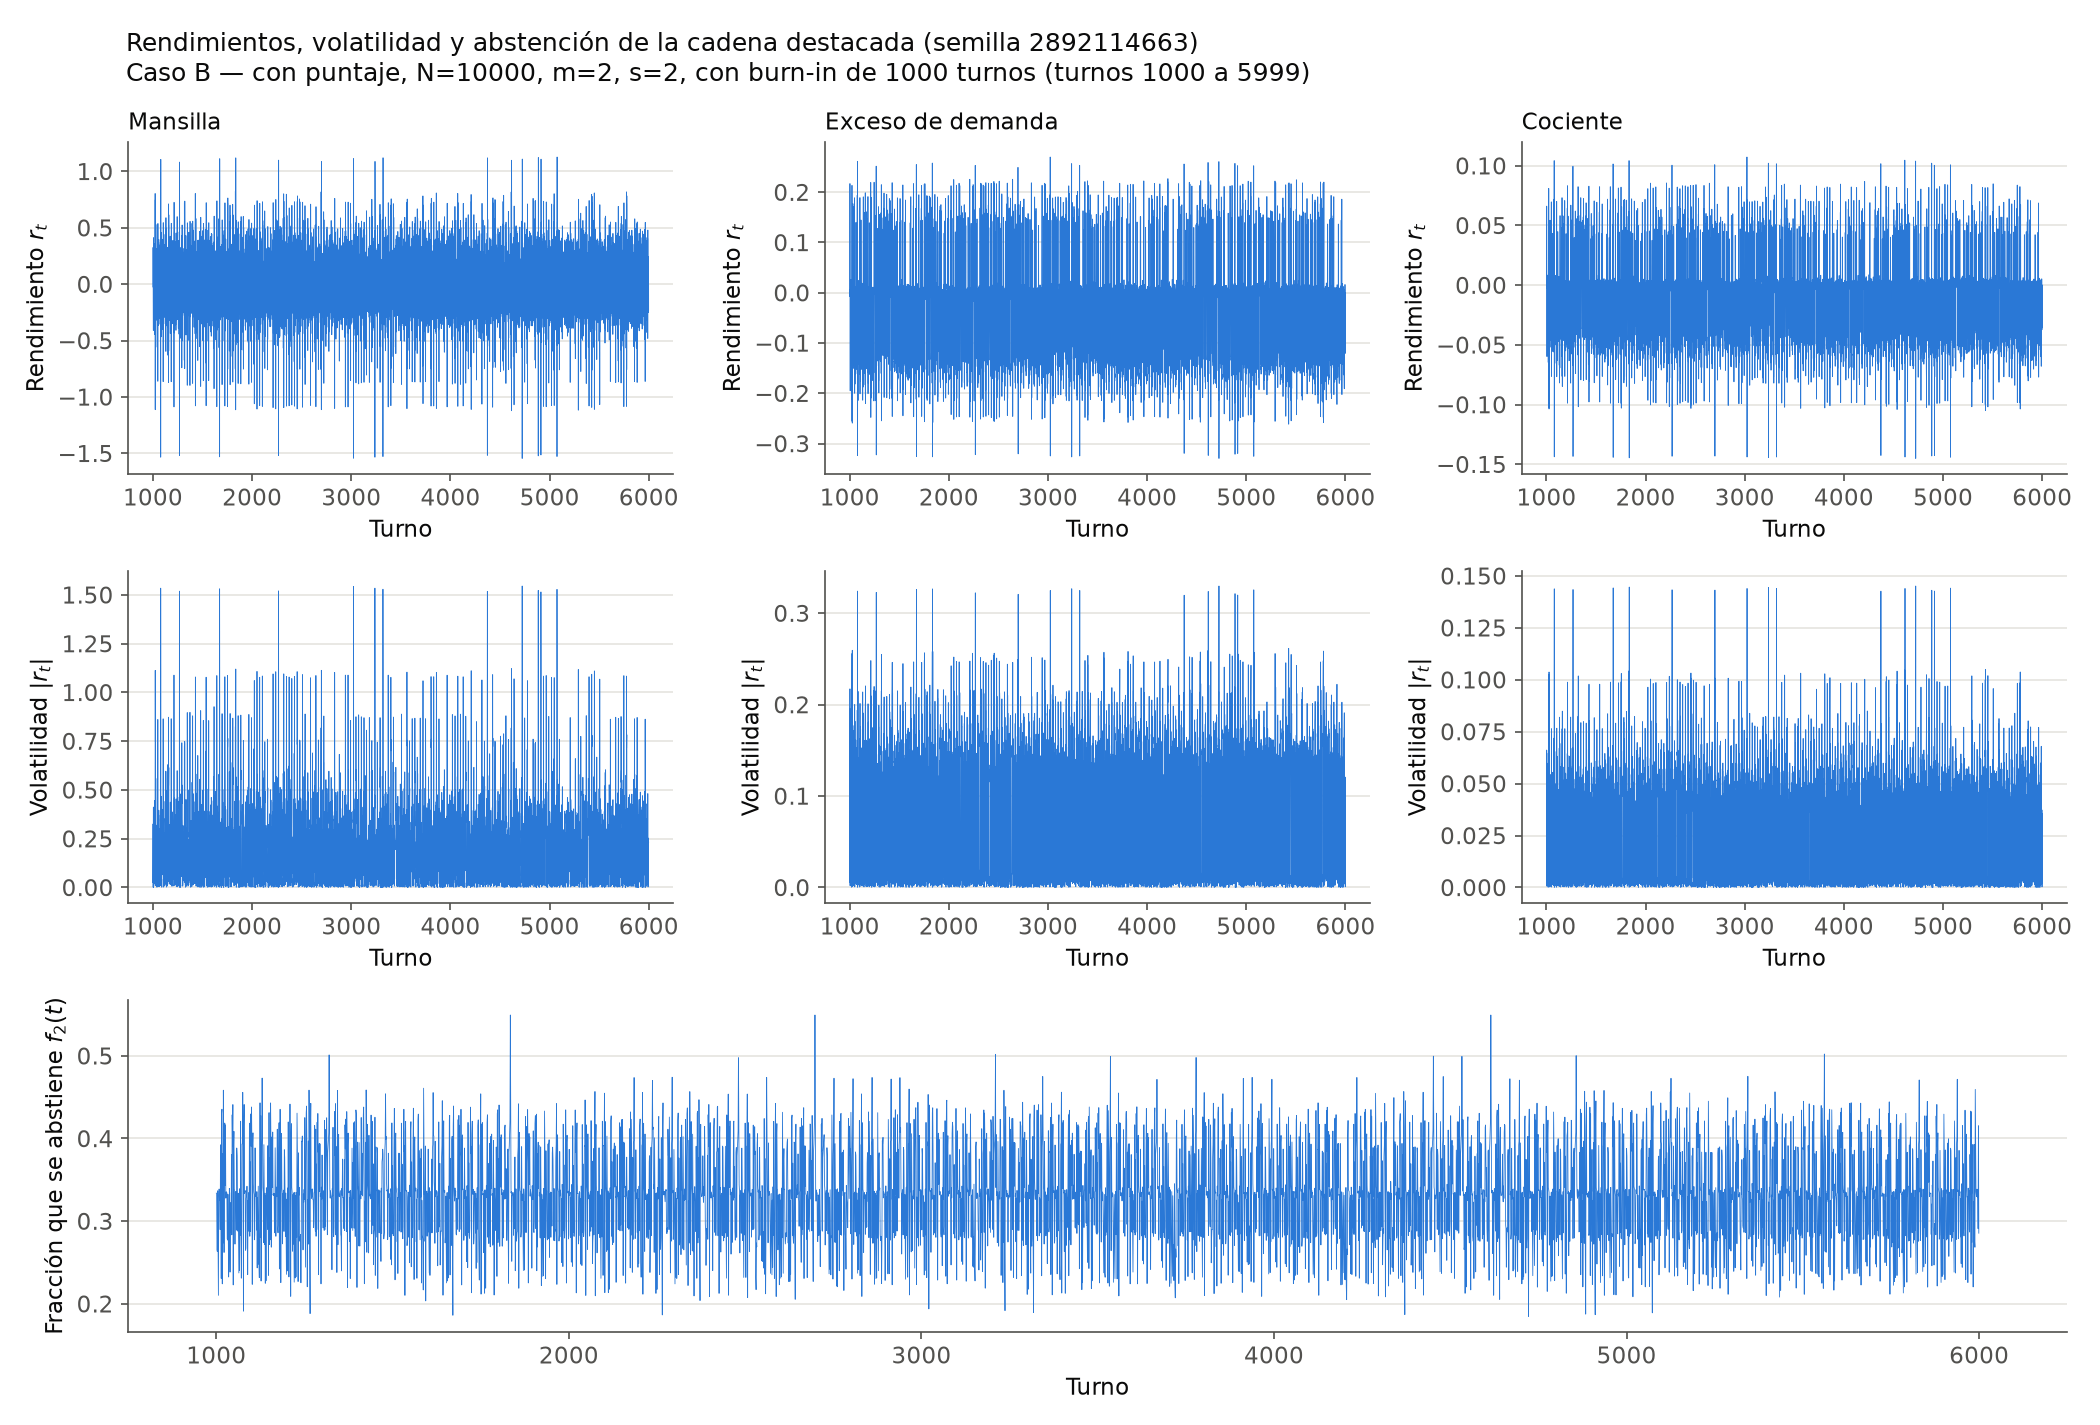
\includegraphics[width=0.85\textwidth]{figuras/Fase9_series_casoB_N10000_m2_s2_con_puntaje_T6000_regla_nueva_con_burnin1000.png}
\caption{Caso B: rendimientos, volatilidad y fracción que se abstiene de la cadena destacada, con burn-in.}
\end{figure}

\begin{figure}[H]
\centering
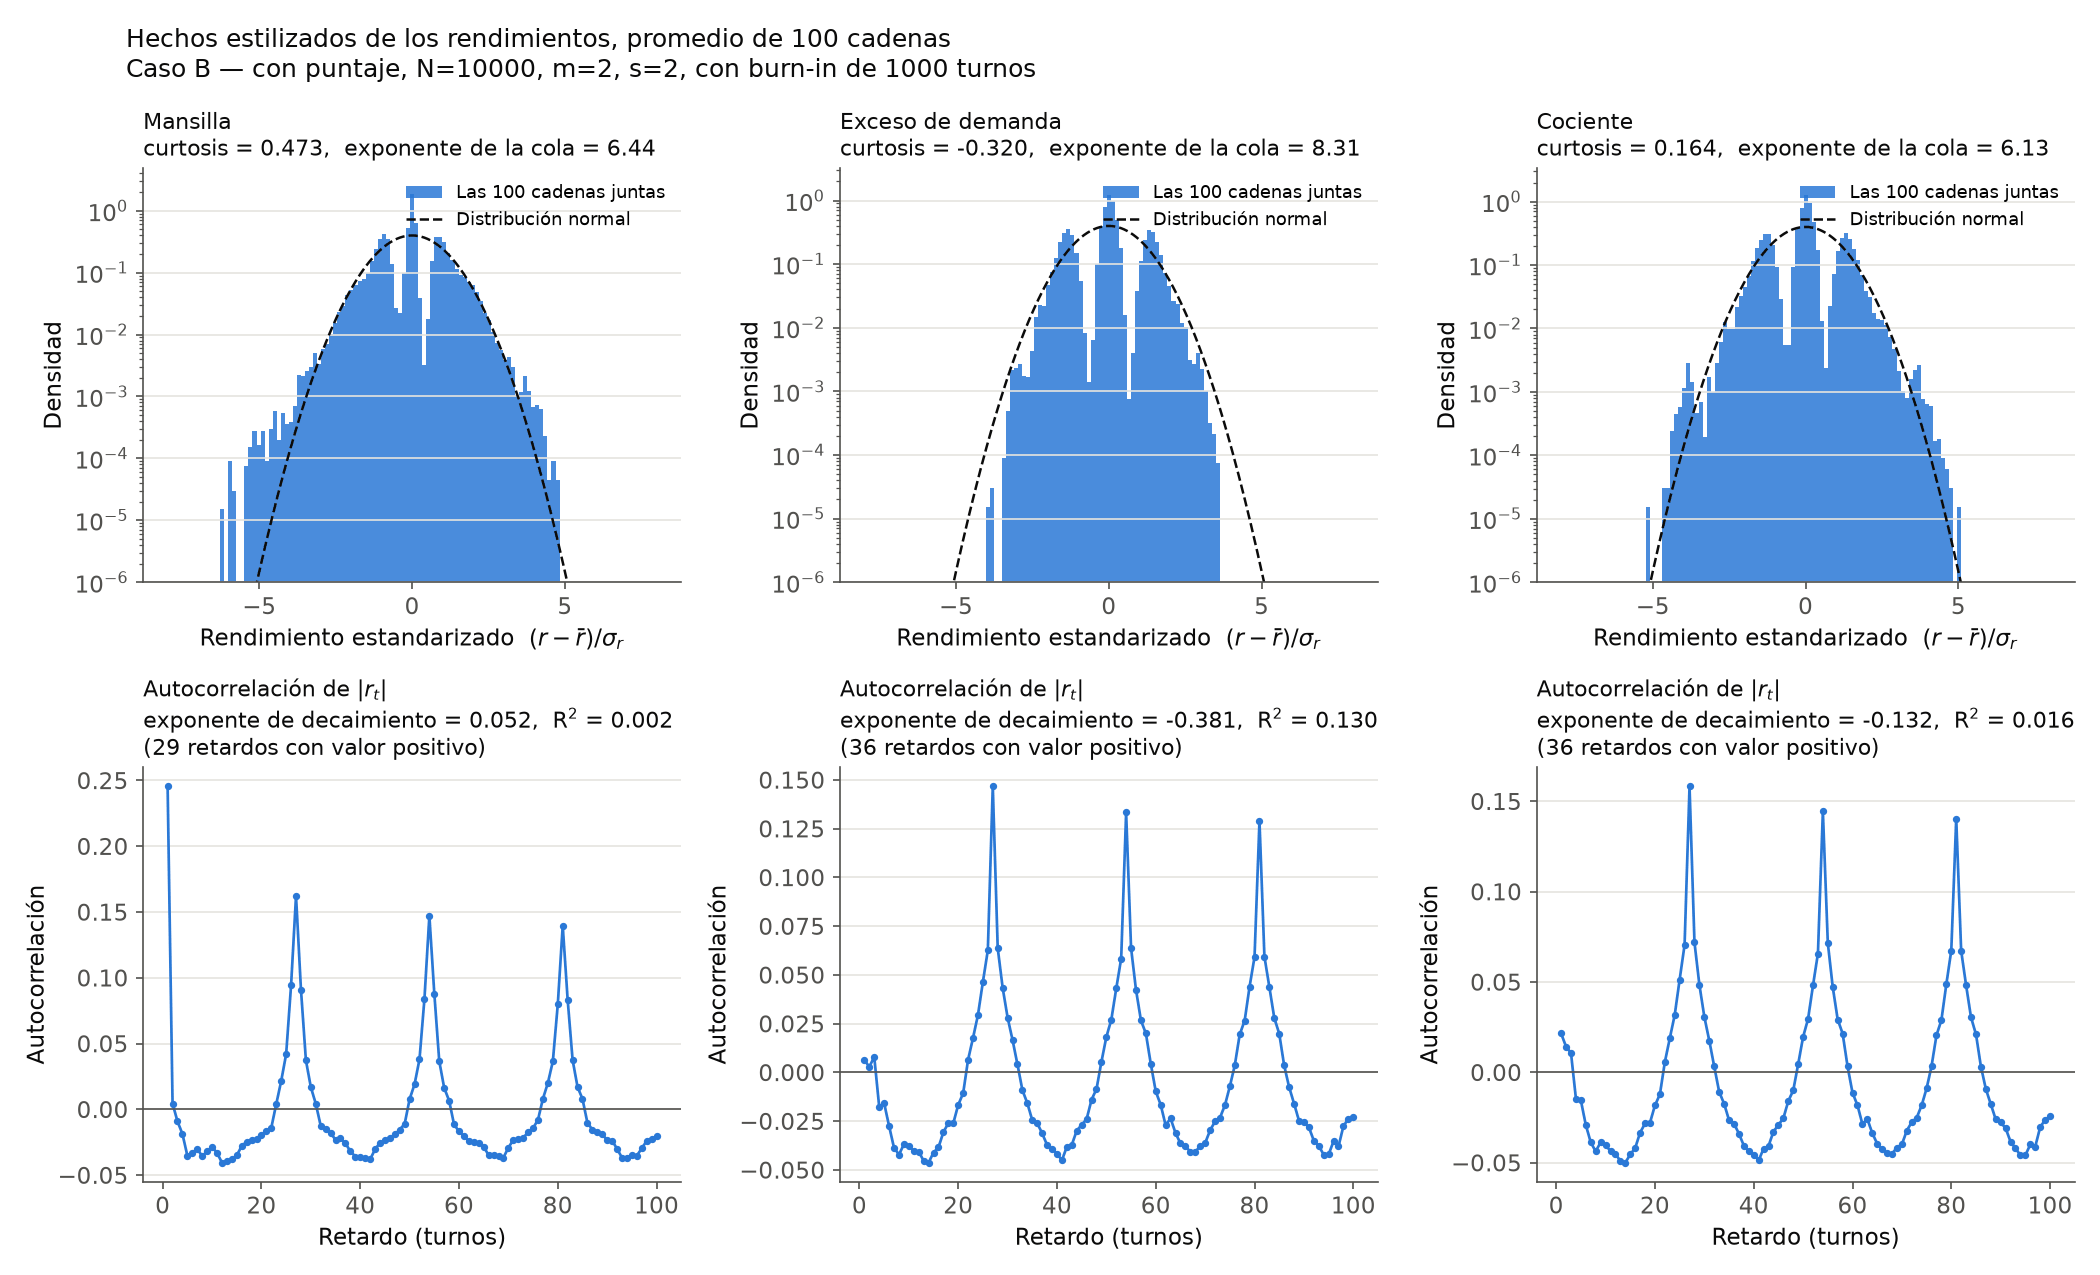
\includegraphics[width=0.85\textwidth]{figuras/Fase9_hechos_estilizados_casoB_N10000_m2_s2_con_puntaje_T6000_regla_nueva_con_burnin1000.png}
\caption{Caso B: hechos estilizados (distribución de los rendimientos y autocorrelación de $|r|$), con burn-in.}
\end{figure}

\begin{figure}[H]
\centering
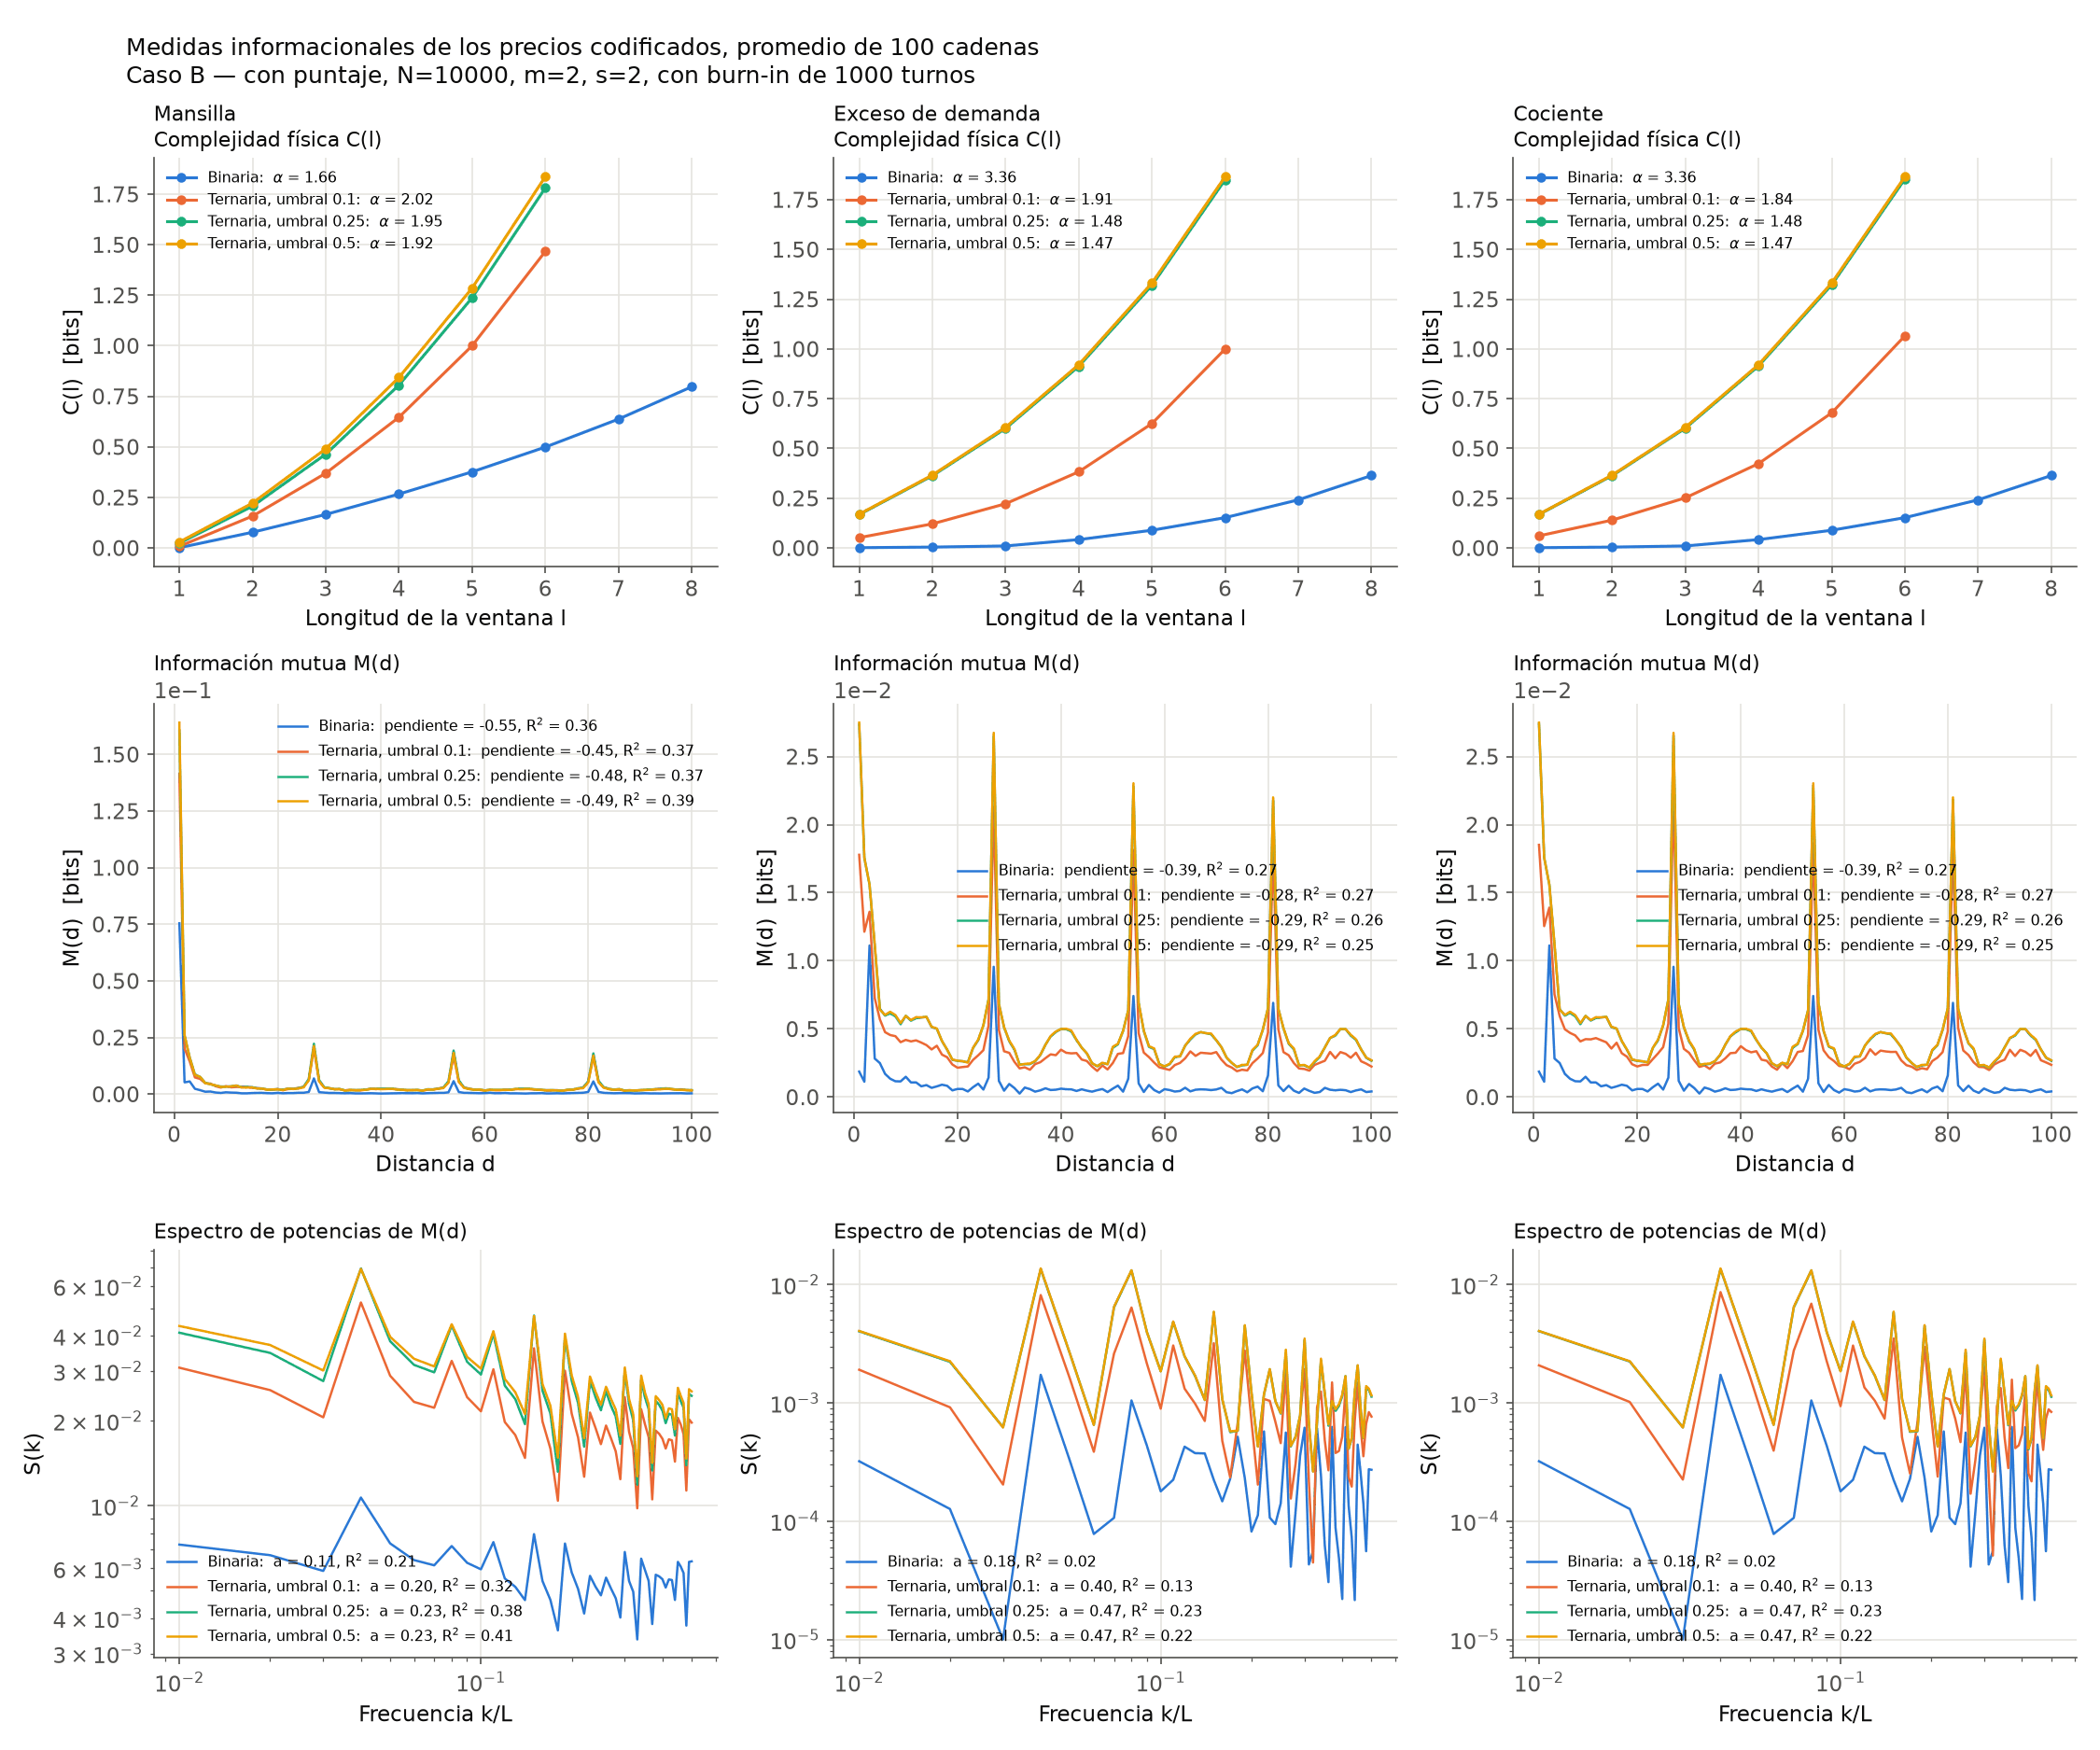
\includegraphics[width=0.85\textwidth]{figuras/Fase9_medidas_informacionales_casoB_N10000_m2_s2_con_puntaje_T6000_regla_nueva_con_burnin1000.png}
\caption{Caso B: medidas informacionales de los precios codificados, con burn-in.}
\end{figure}

\clearpage
\subsection{Caso C: $m=3$, sin puntaje}
\begin{figure}[H]
\centering
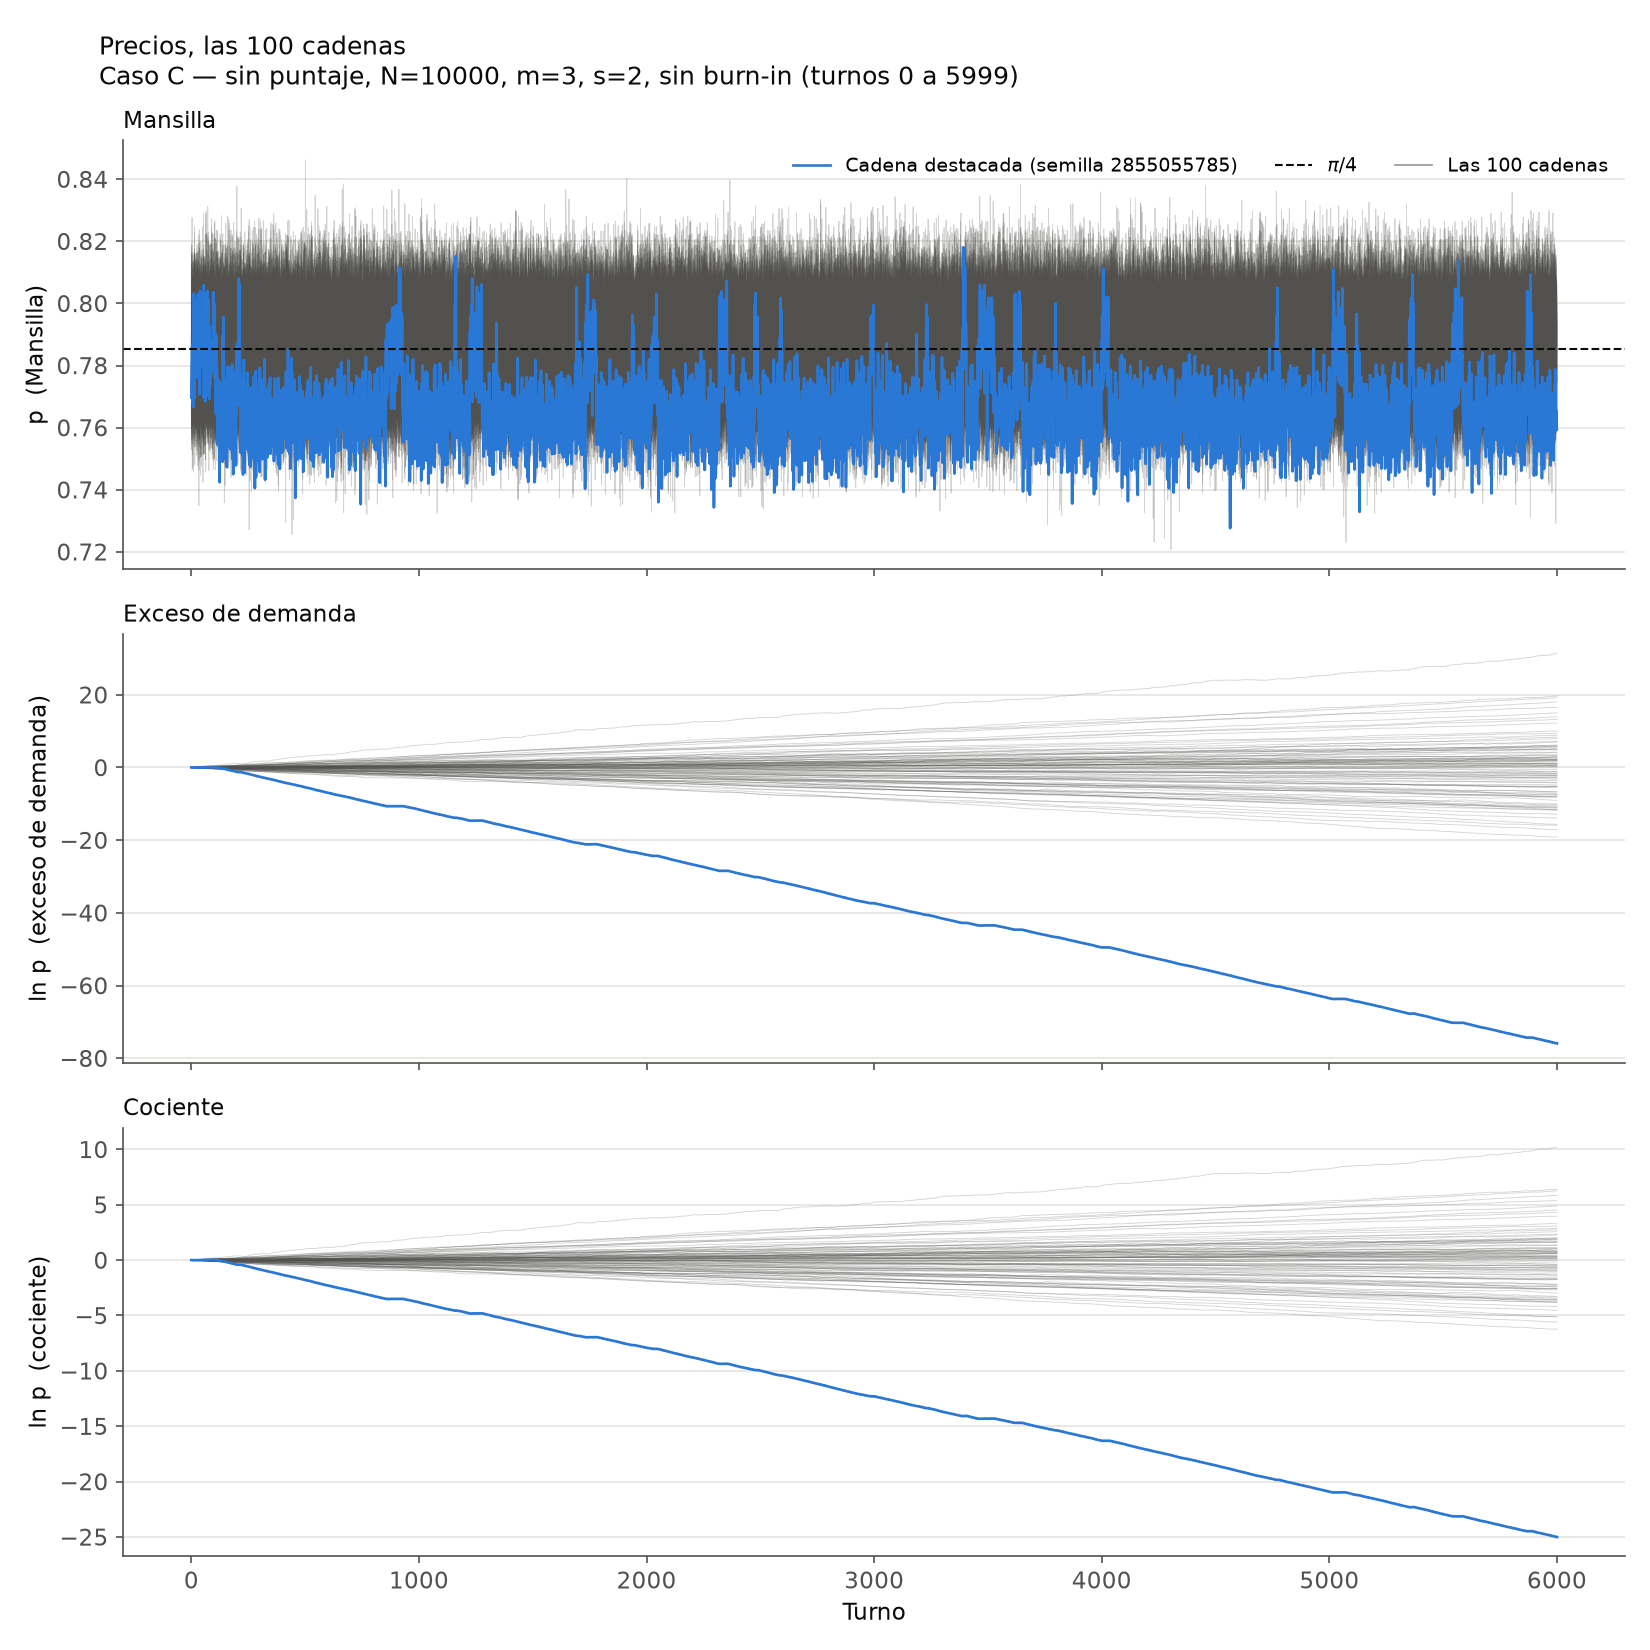
\includegraphics[width=0.49\textwidth]{figuras/Fase9_precios_conjunto_casoC_N10000_m3_s2_sin_puntaje_T6000_regla_nueva_sin_burnin.png}\hfill
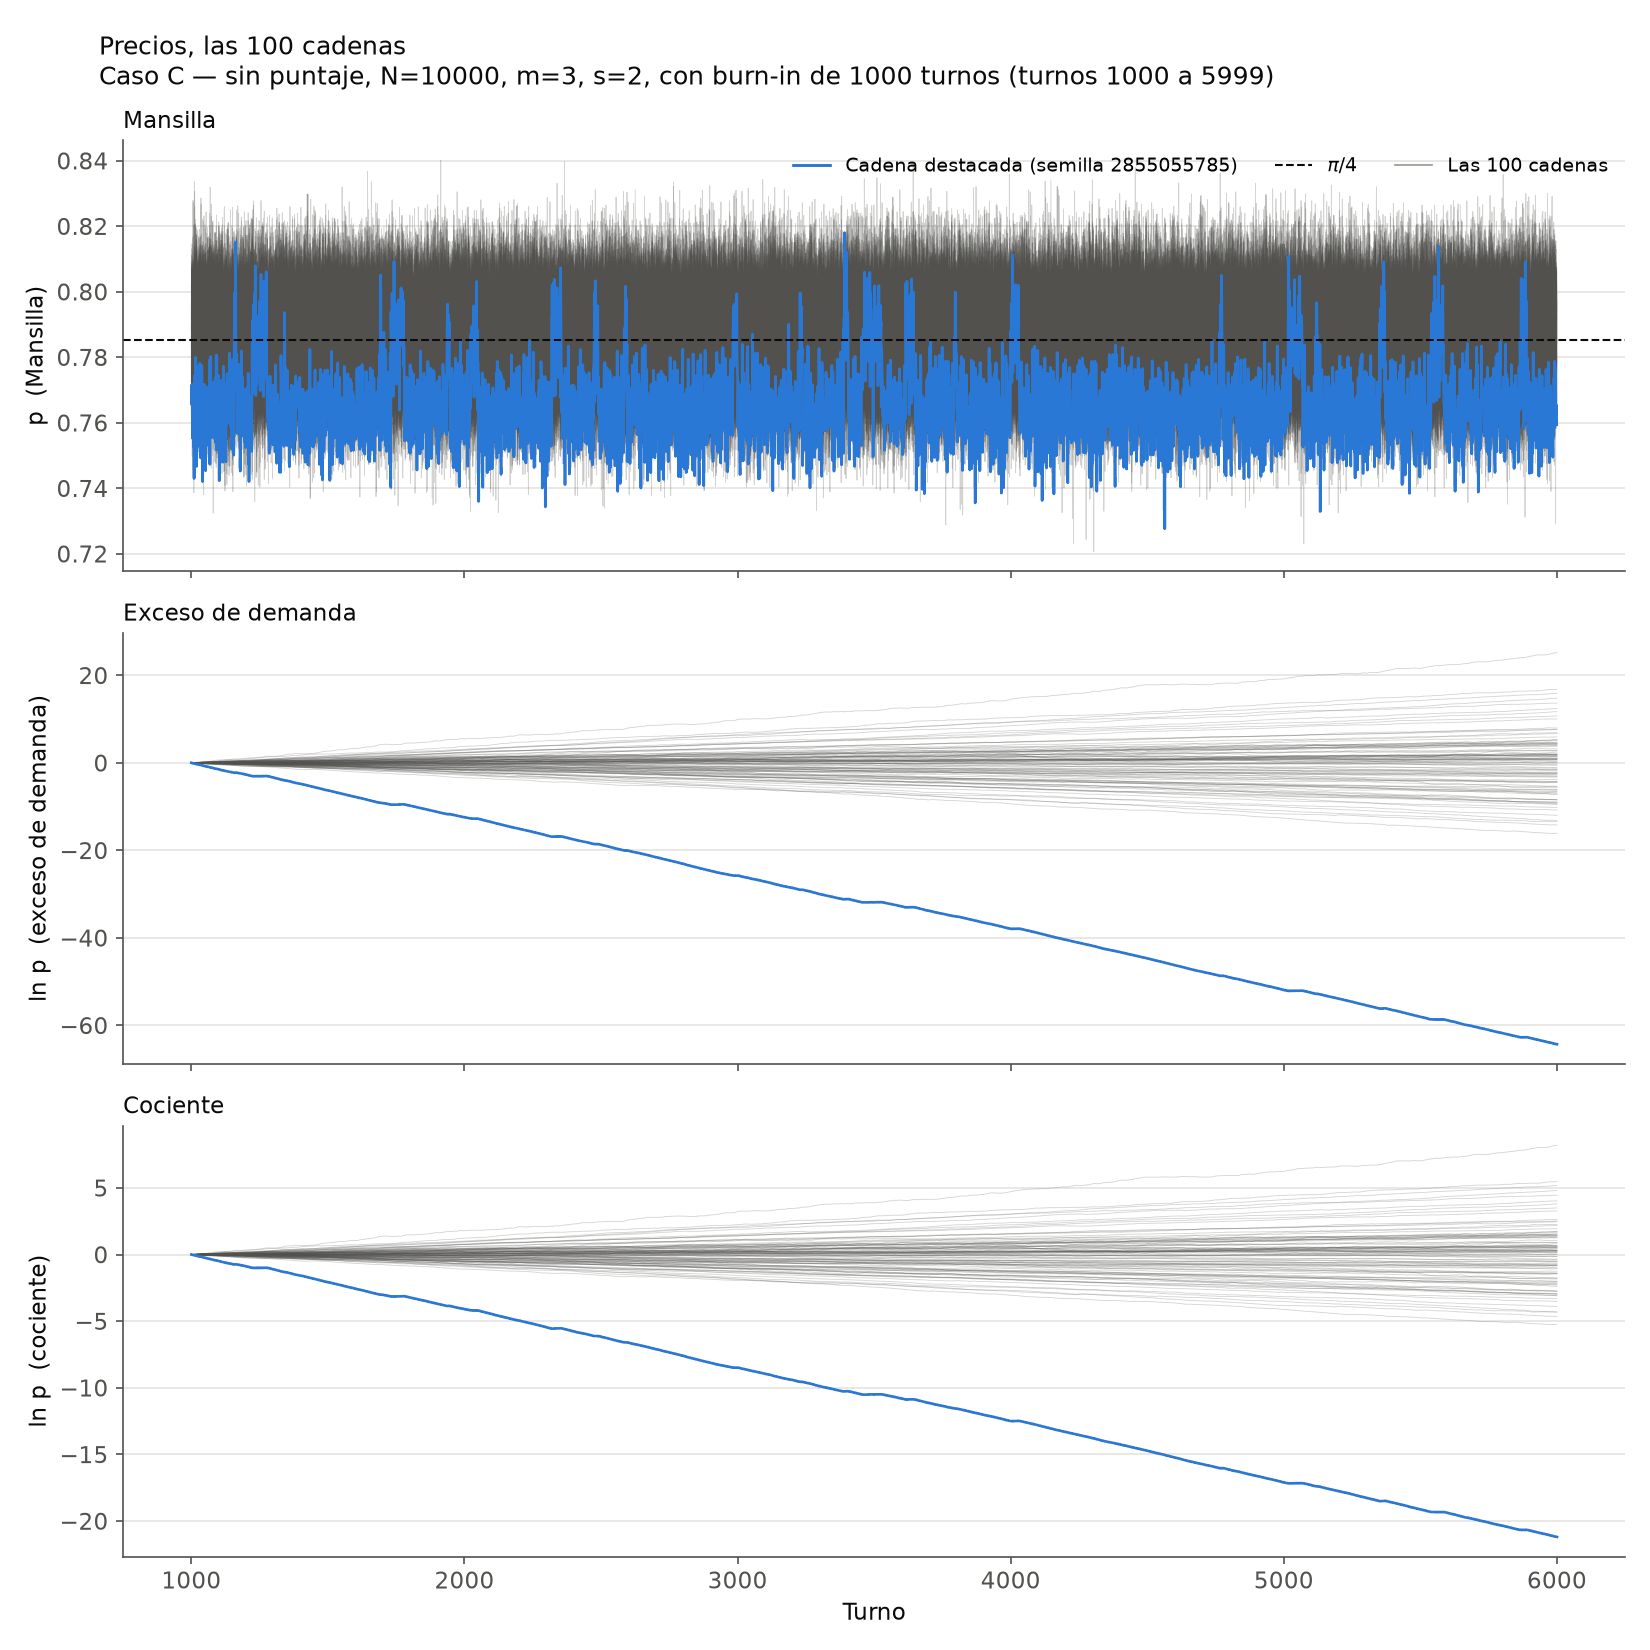
\includegraphics[width=0.49\textwidth]{figuras/Fase9_precios_conjunto_casoC_N10000_m3_s2_sin_puntaje_T6000_regla_nueva_con_burnin1000.png}
\caption{Caso C, $N=10000$: conjunto de precios sin burn-in (izquierda) y con burn-in (derecha).}
\end{figure}

\begin{figure}[H]
\centering
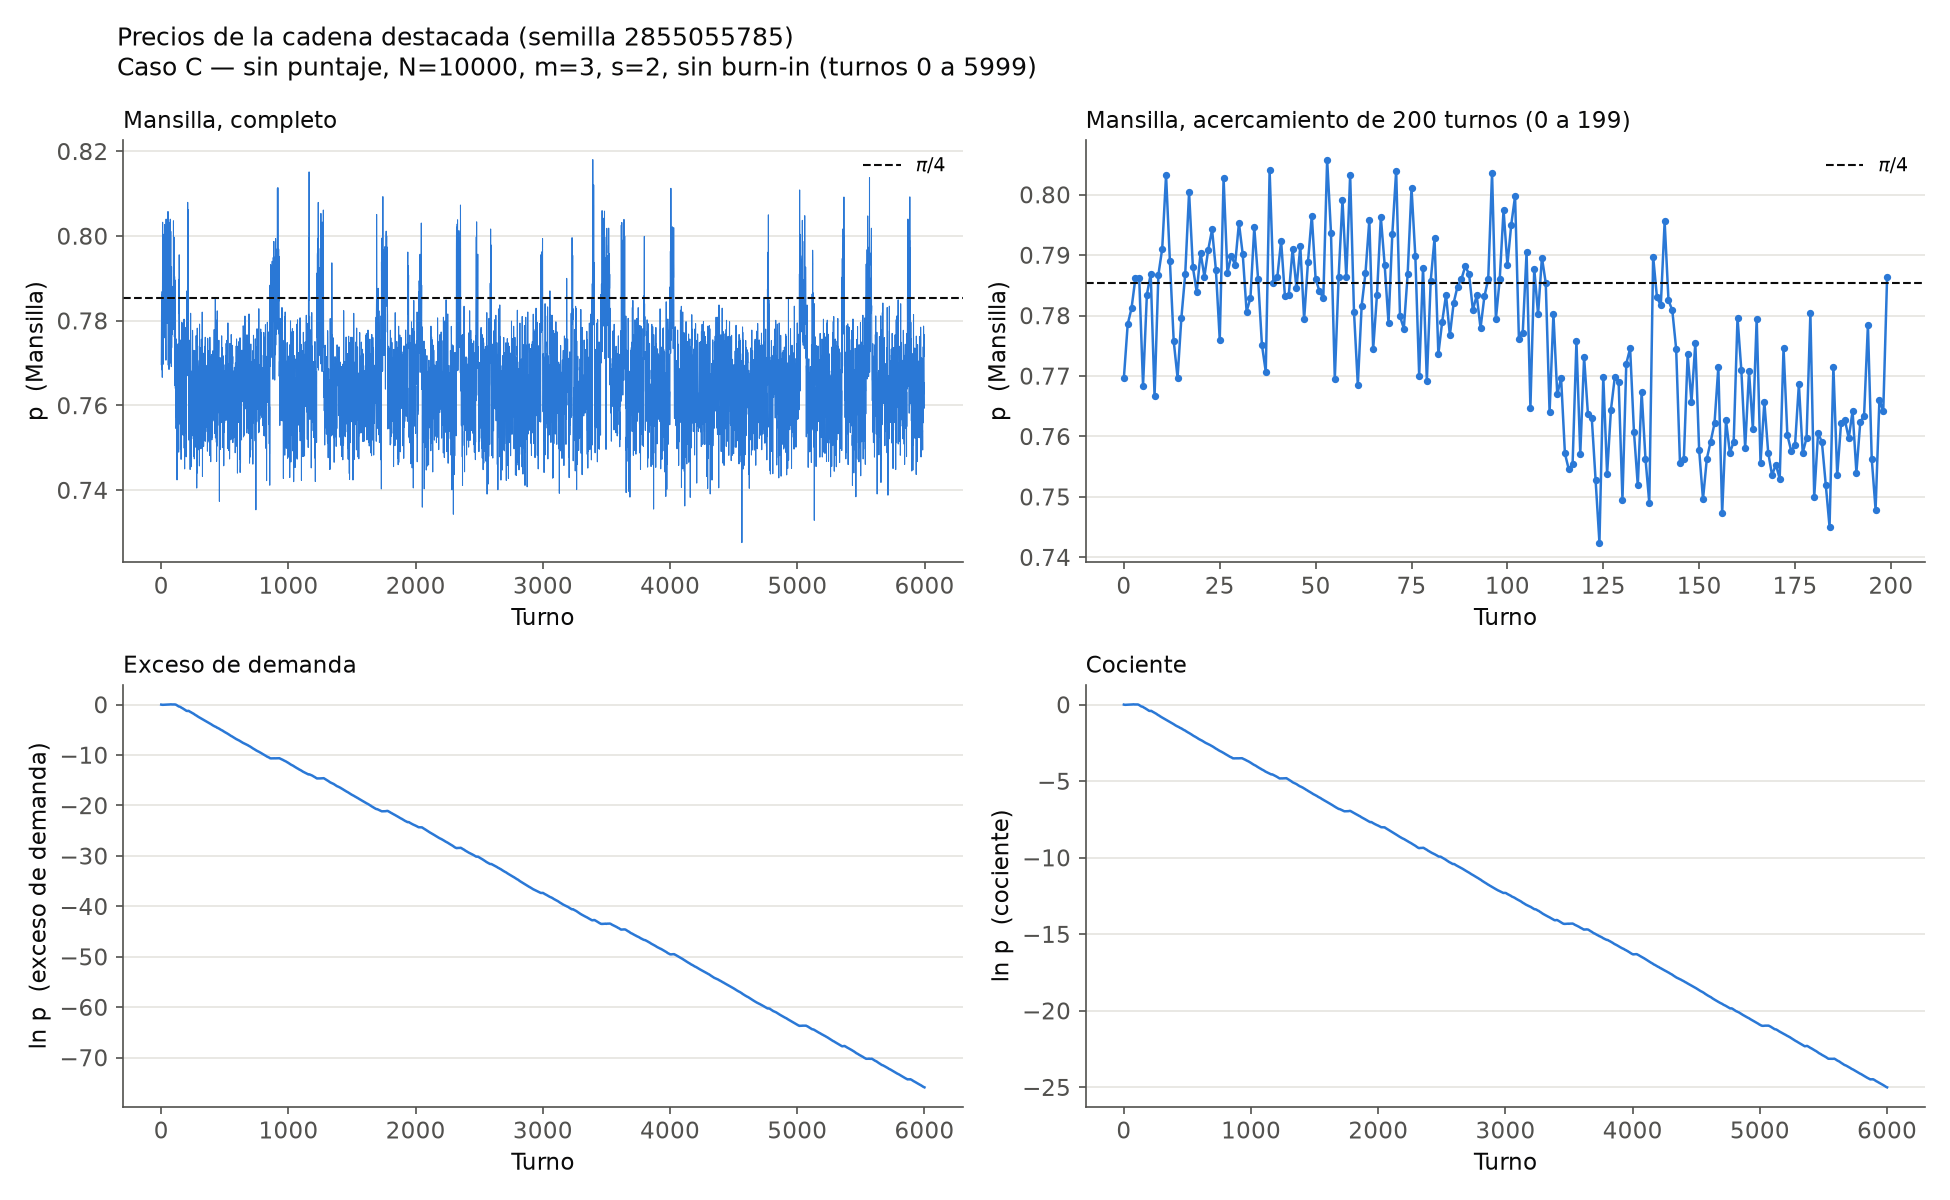
\includegraphics[width=0.49\textwidth]{figuras/Fase9_precios_detalle_casoC_N10000_m3_s2_sin_puntaje_T6000_regla_nueva_sin_burnin.png}\hfill
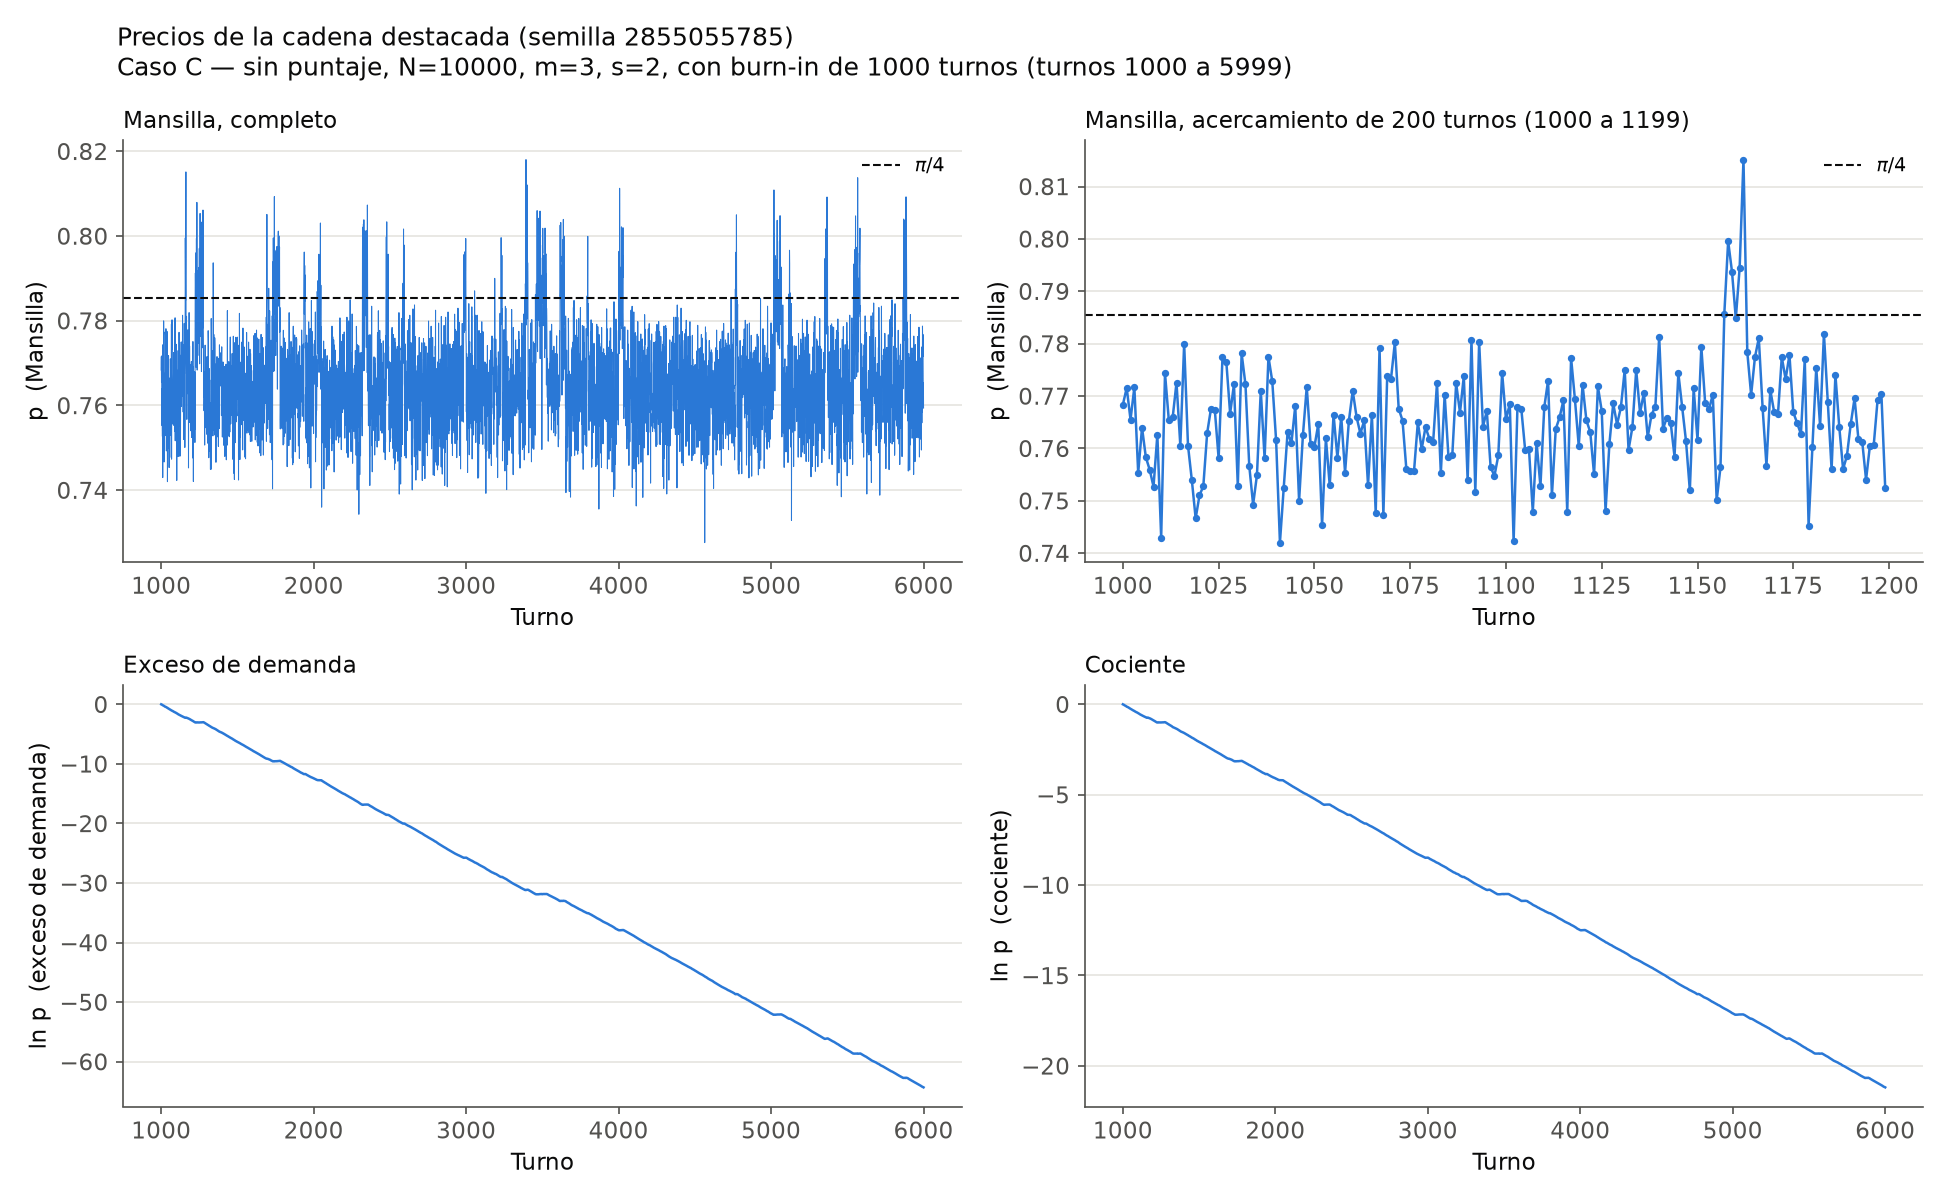
\includegraphics[width=0.49\textwidth]{figuras/Fase9_precios_detalle_casoC_N10000_m3_s2_sin_puntaje_T6000_regla_nueva_con_burnin1000.png}
\caption{Caso C, $N=10000$: detalle de la cadena destacada sin burn-in (izquierda) y con burn-in (derecha).}
\end{figure}

\begin{figure}[H]
\centering
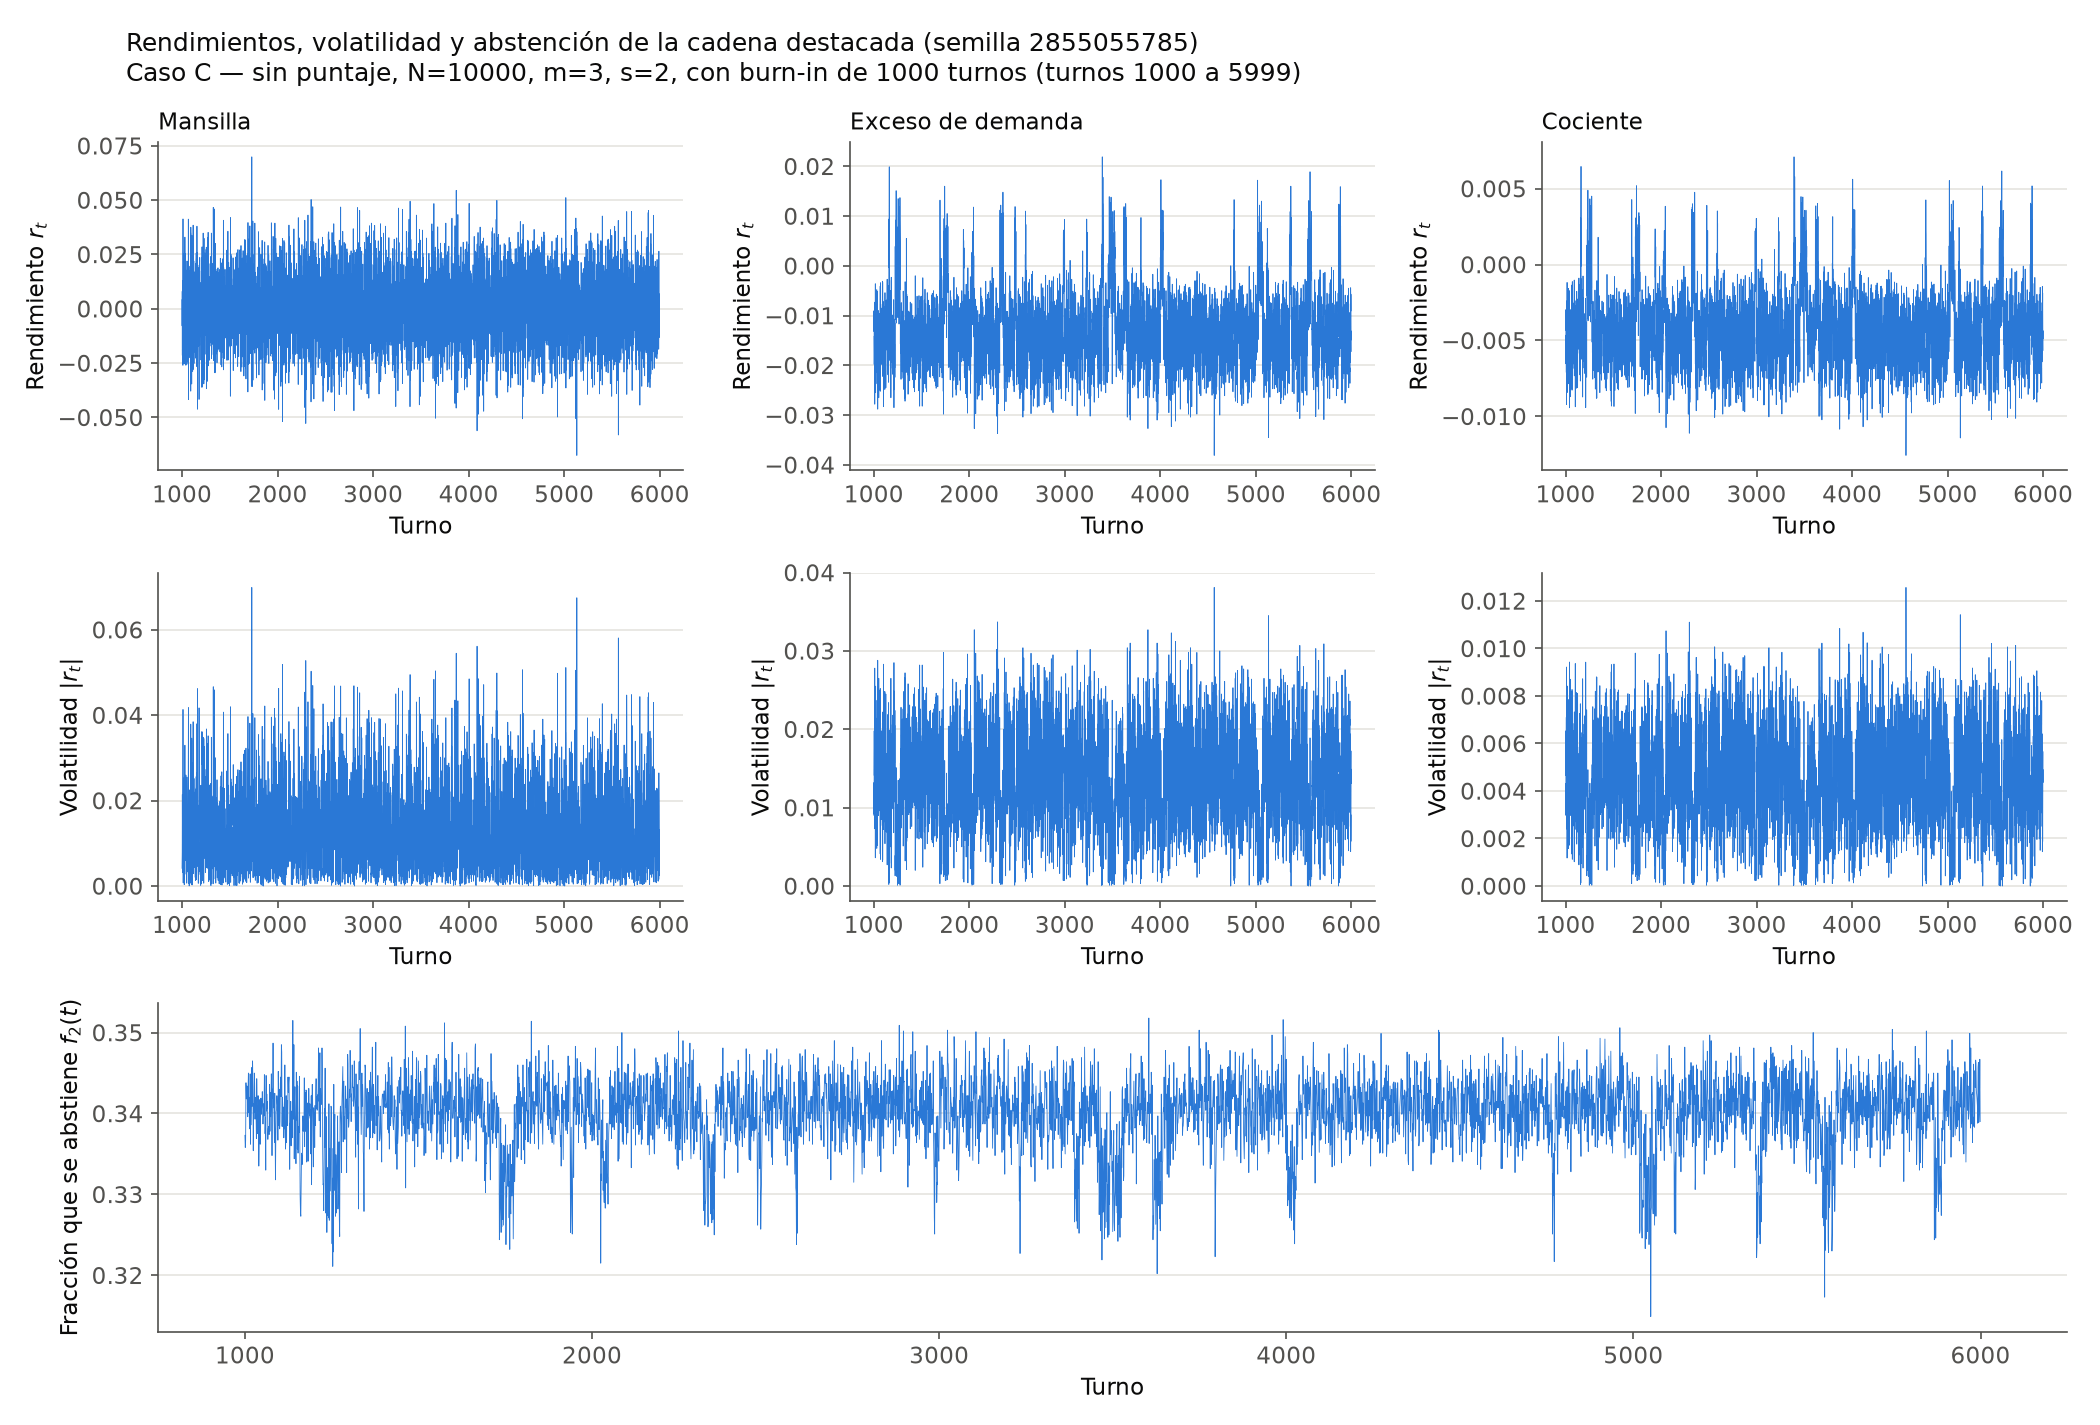
\includegraphics[width=0.85\textwidth]{figuras/Fase9_series_casoC_N10000_m3_s2_sin_puntaje_T6000_regla_nueva_con_burnin1000.png}
\caption{Caso C: rendimientos, volatilidad y fracción que se abstiene de la cadena destacada, con burn-in.}
\end{figure}

\begin{figure}[H]
\centering
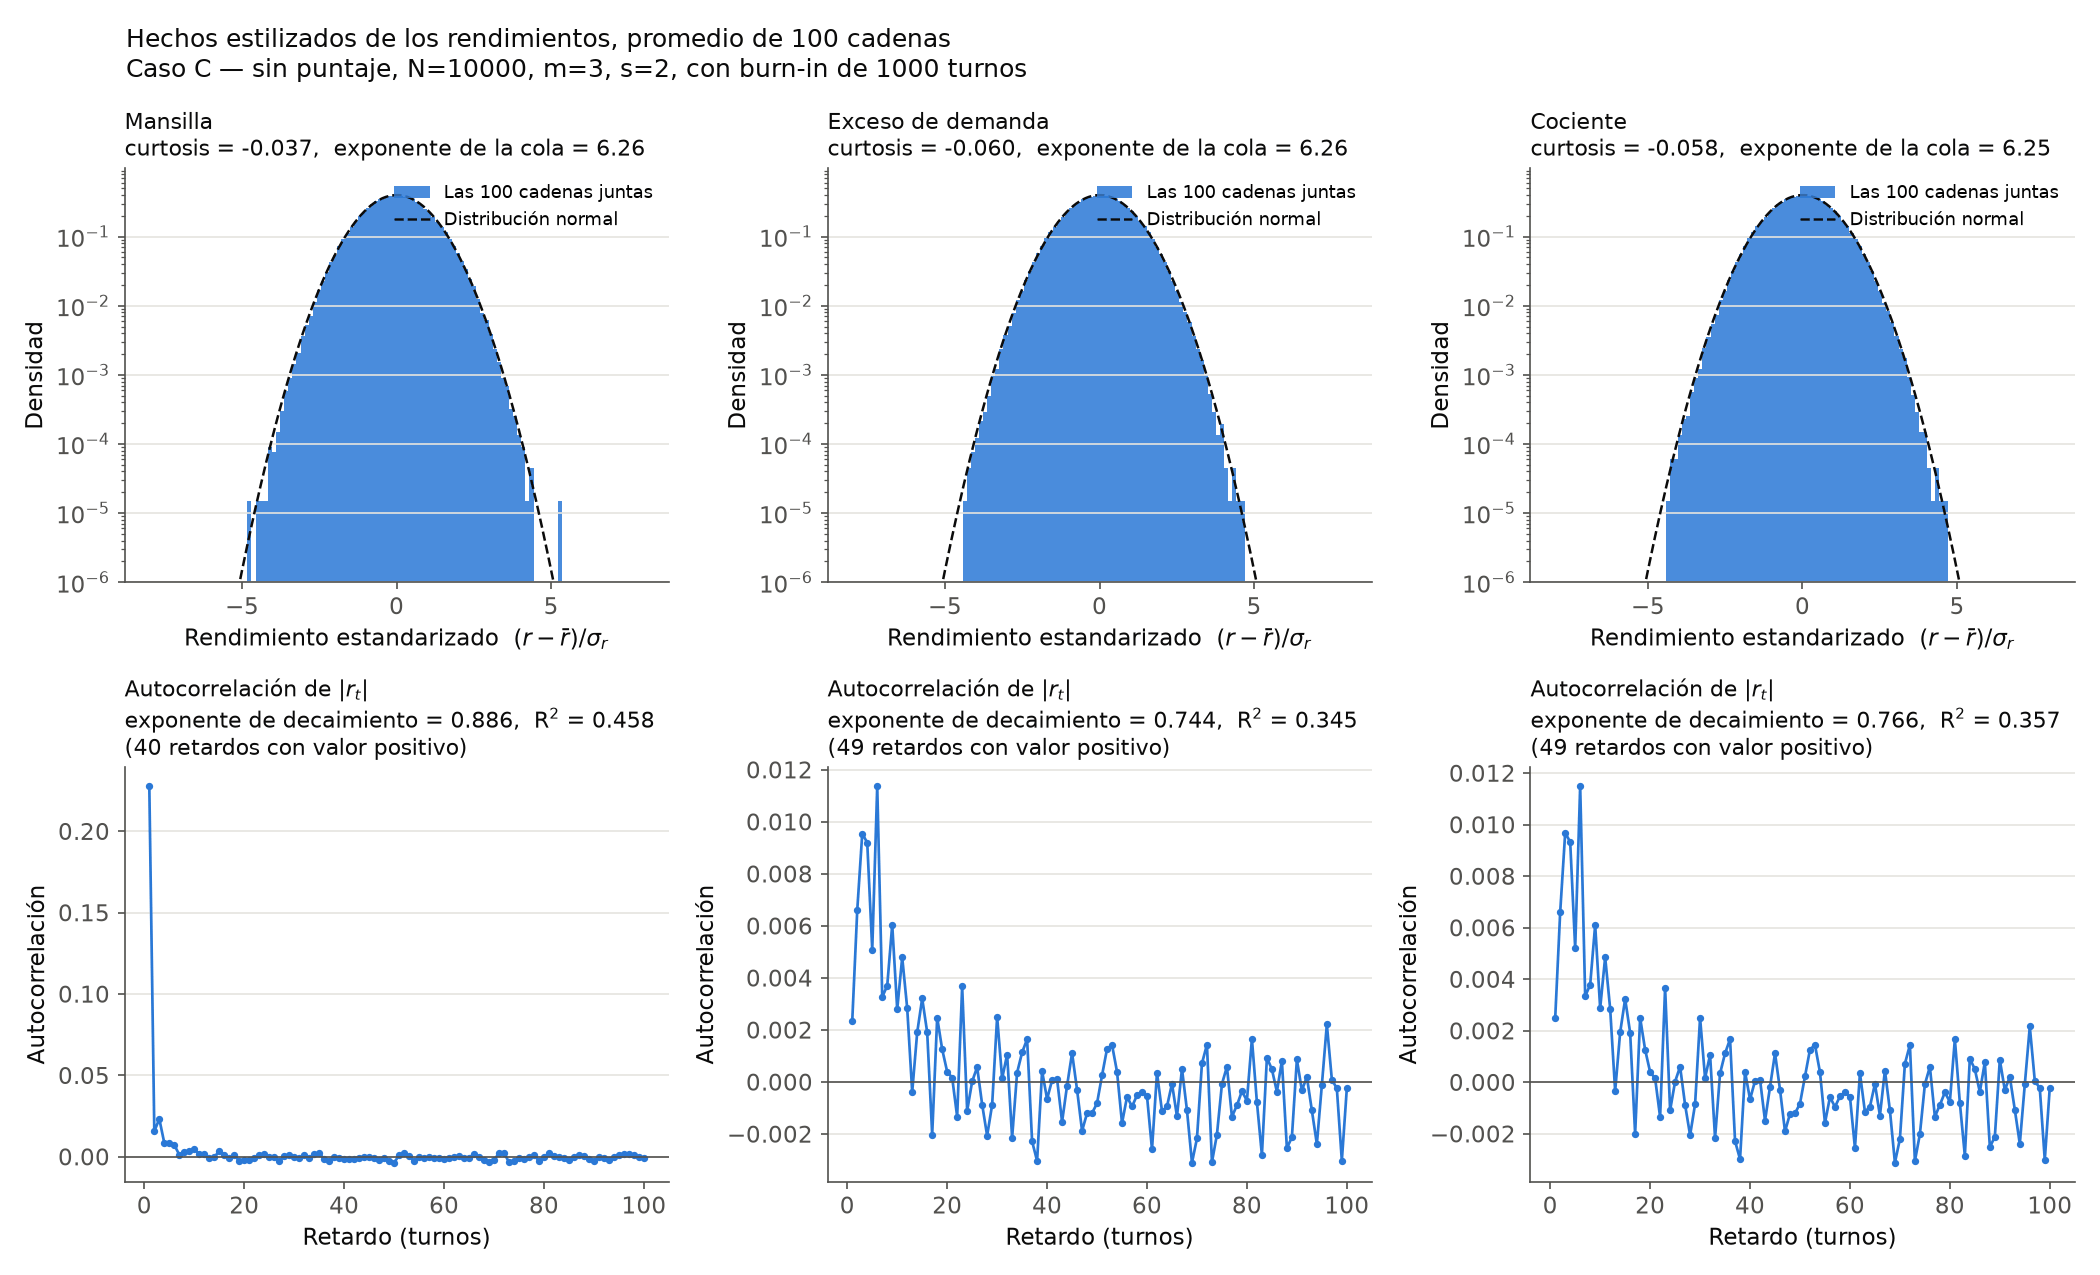
\includegraphics[width=0.85\textwidth]{figuras/Fase9_hechos_estilizados_casoC_N10000_m3_s2_sin_puntaje_T6000_regla_nueva_con_burnin1000.png}
\caption{Caso C: hechos estilizados (distribución de los rendimientos y autocorrelación de $|r|$), con burn-in.}
\end{figure}

\begin{figure}[H]
\centering
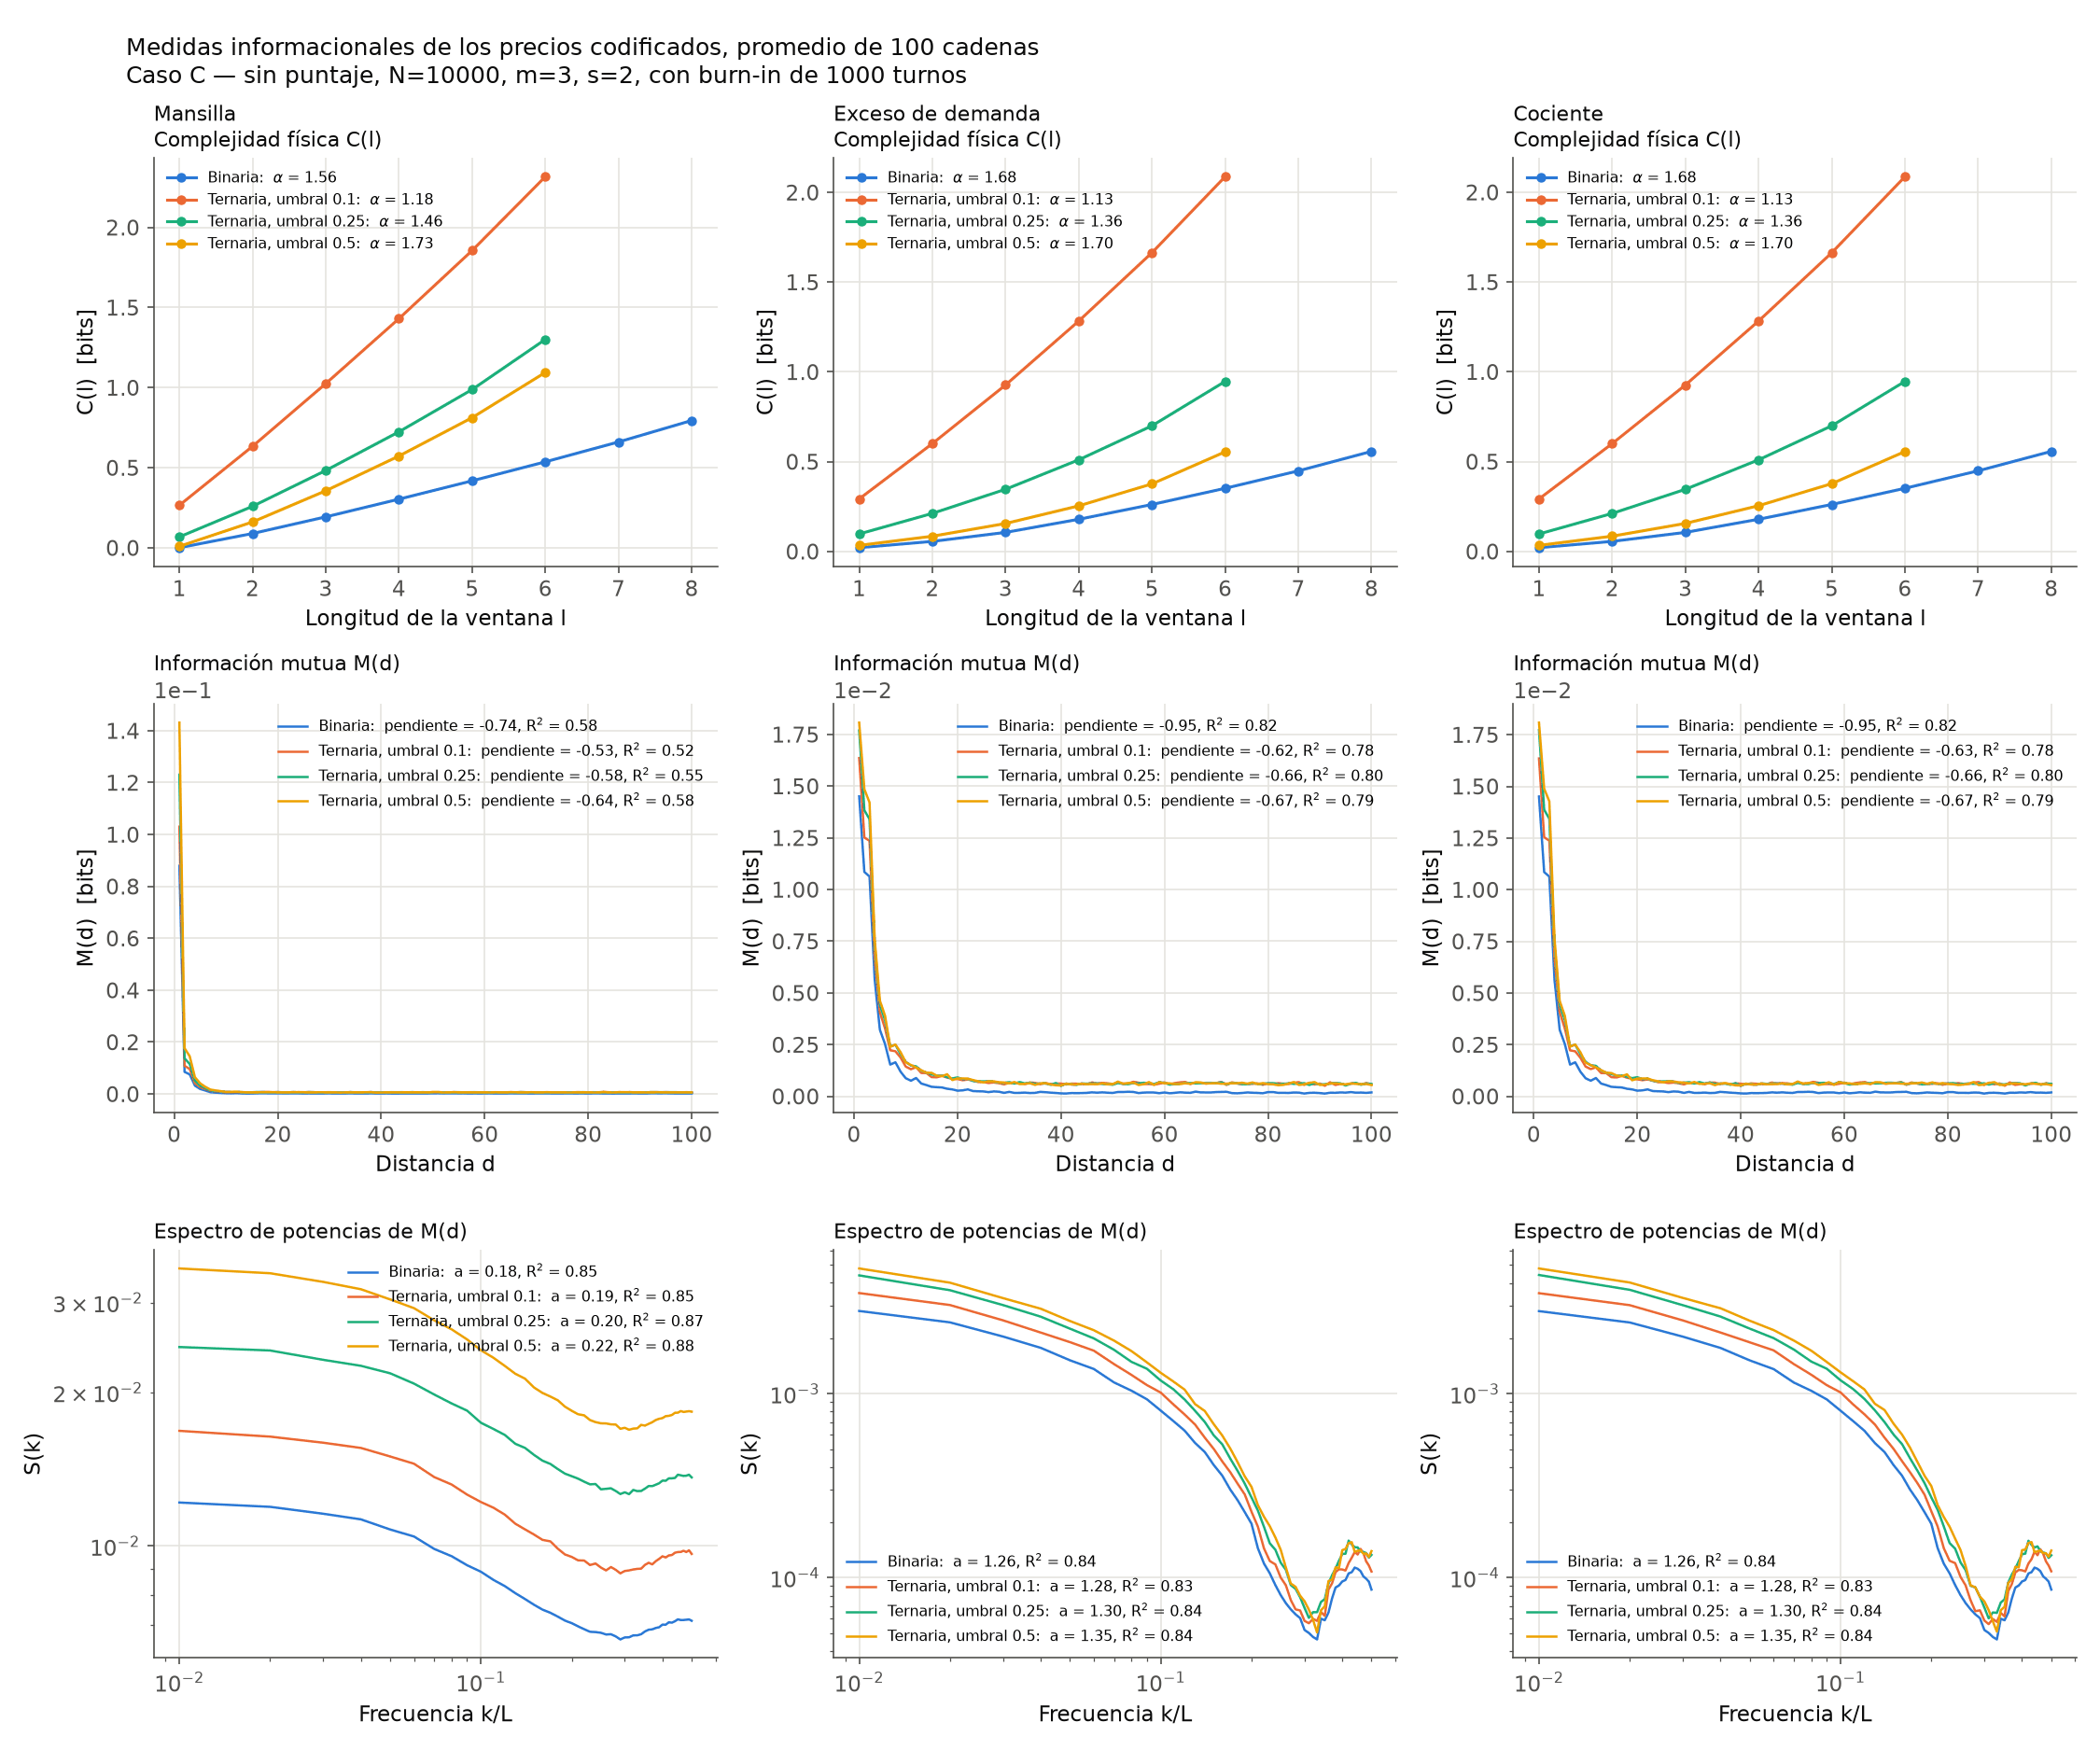
\includegraphics[width=0.85\textwidth]{figuras/Fase9_medidas_informacionales_casoC_N10000_m3_s2_sin_puntaje_T6000_regla_nueva_con_burnin1000.png}
\caption{Caso C: medidas informacionales de los precios codificados, con burn-in.}
\end{figure}

\clearpage
\subsection{Caso D: $m=3$, con puntaje}
\begin{figure}[H]
\centering
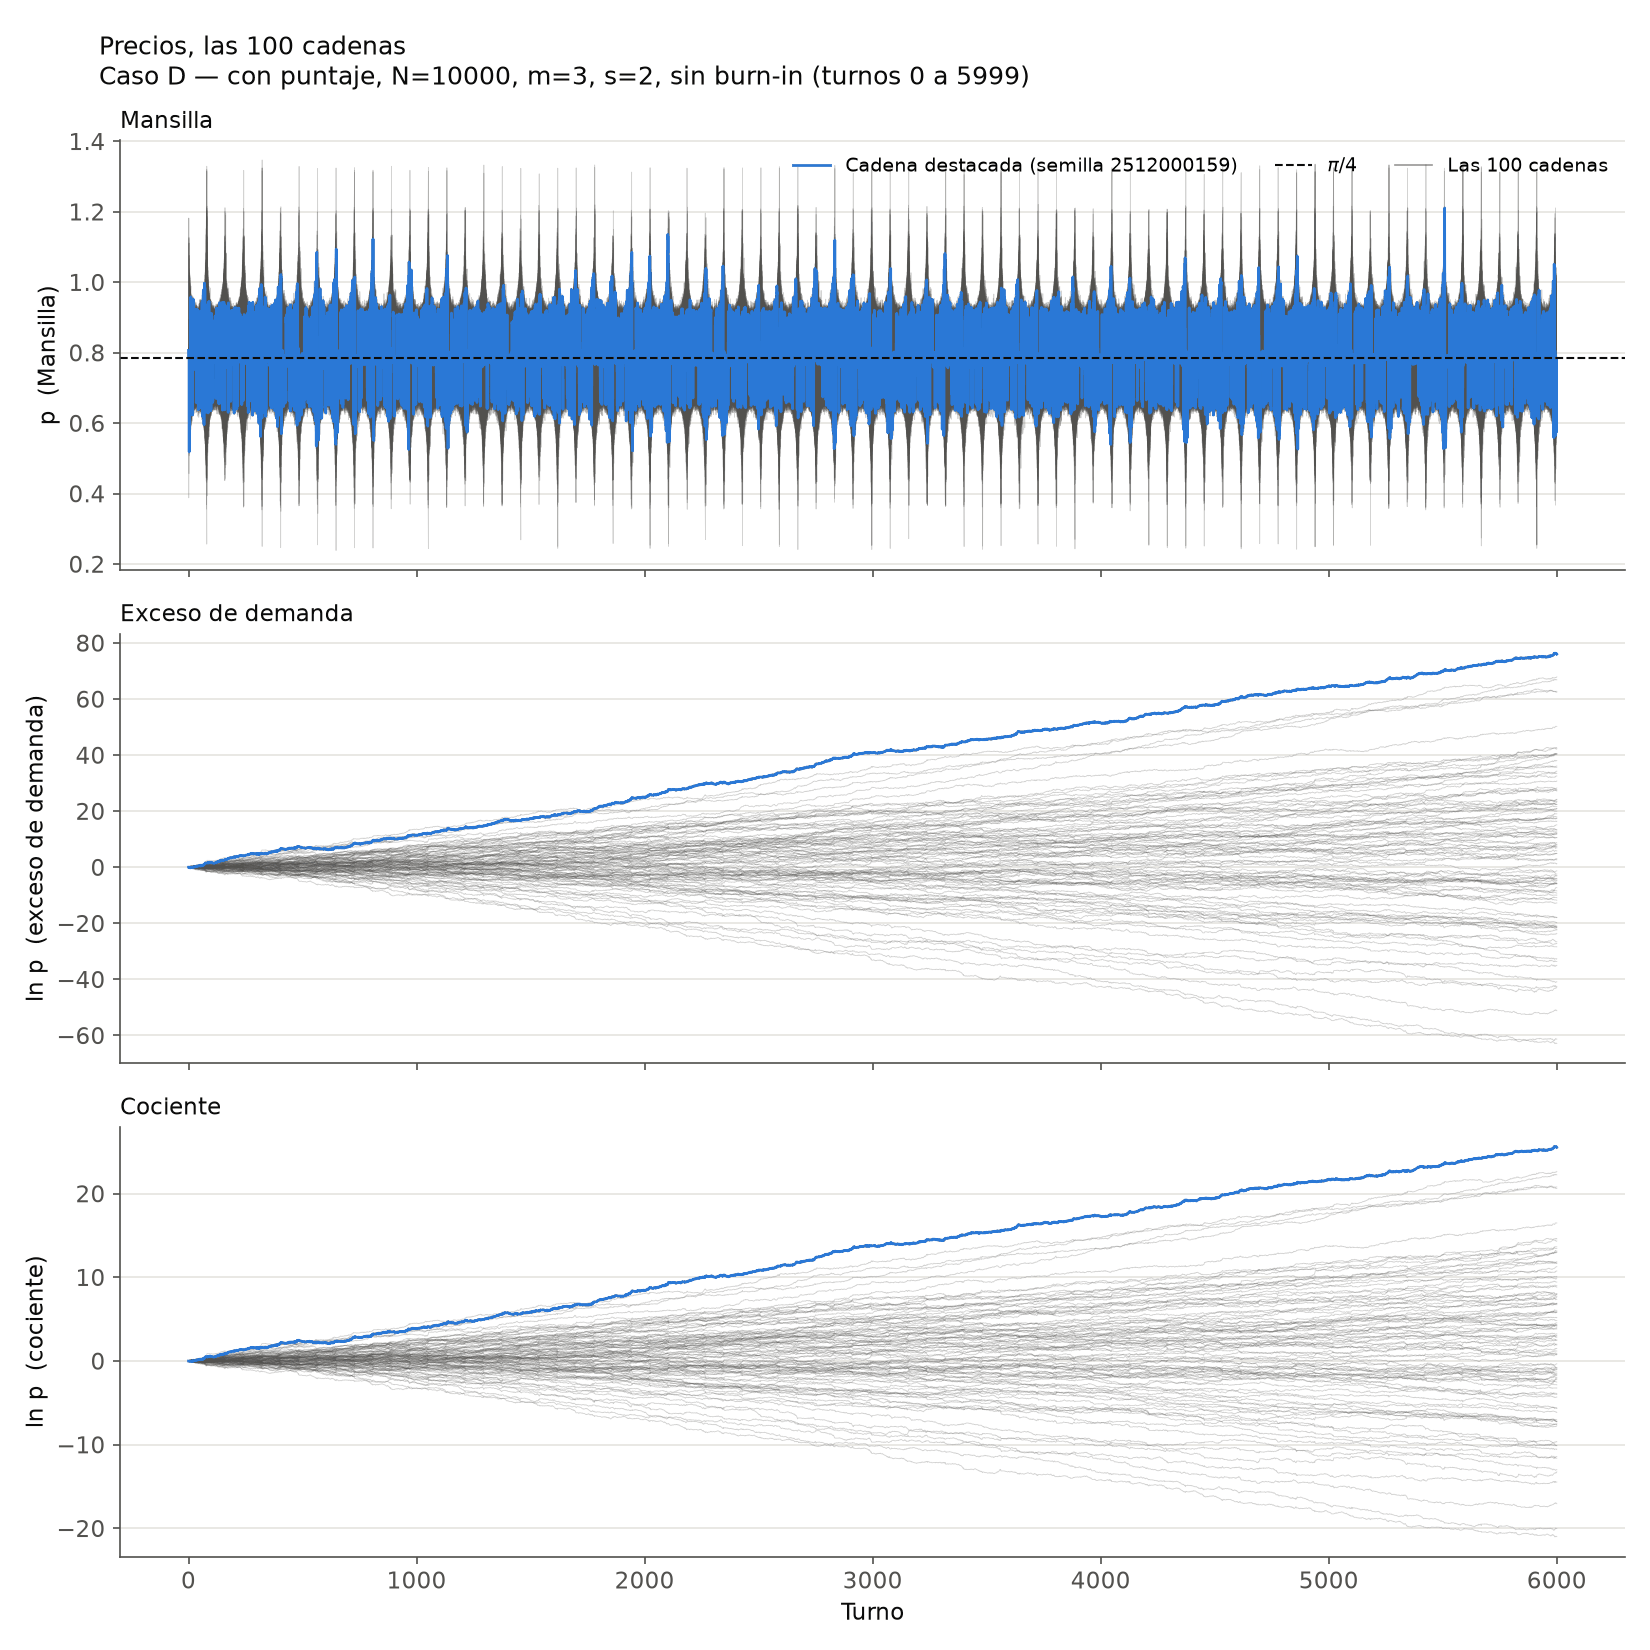
\includegraphics[width=0.49\textwidth]{figuras/Fase9_precios_conjunto_casoD_N10000_m3_s2_con_puntaje_T6000_regla_nueva_sin_burnin.png}\hfill
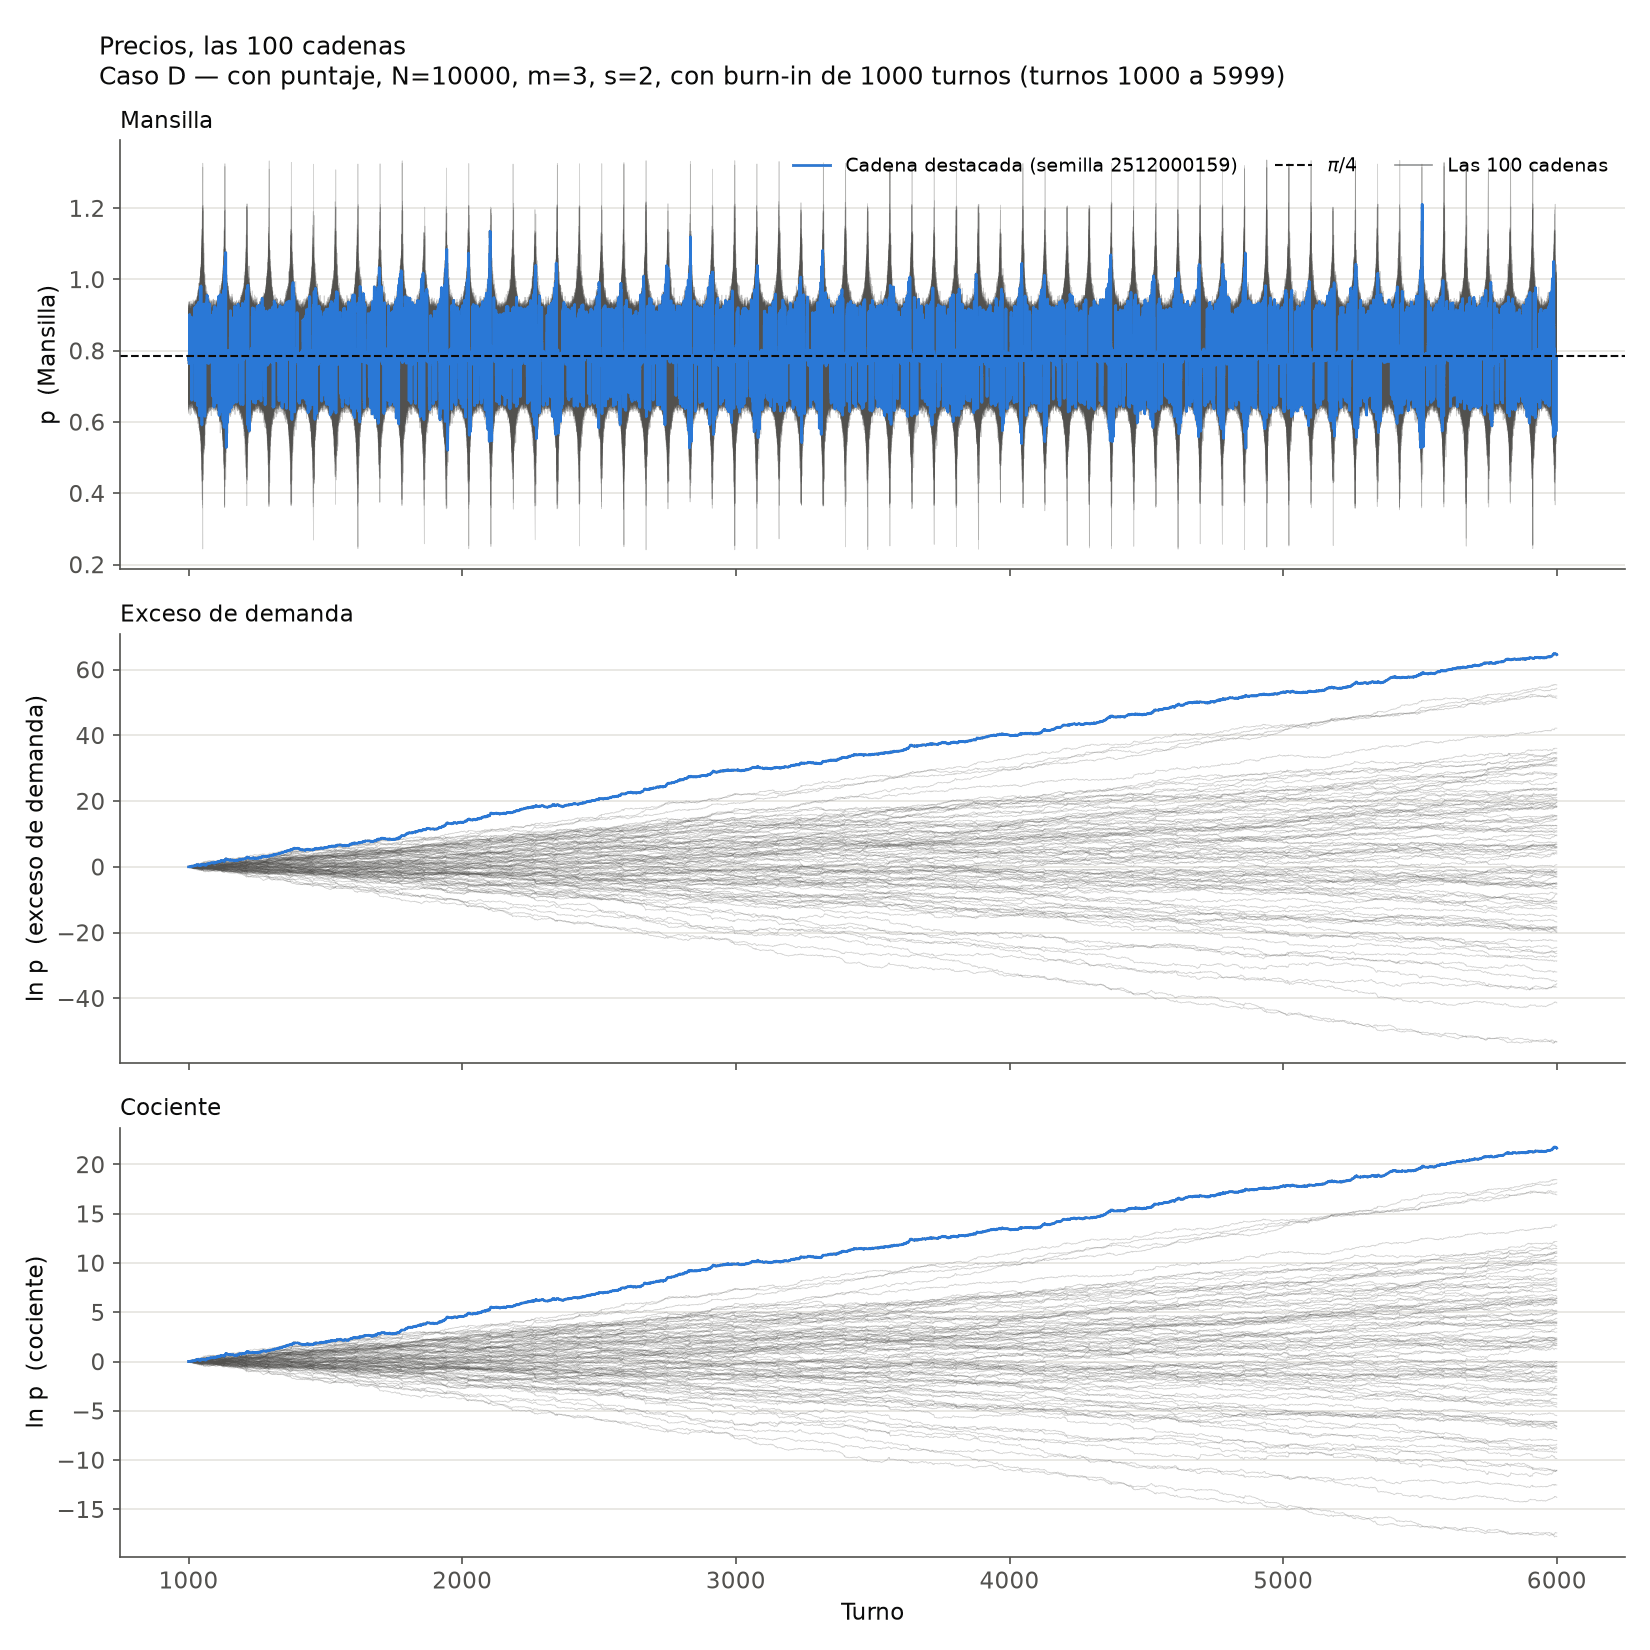
\includegraphics[width=0.49\textwidth]{figuras/Fase9_precios_conjunto_casoD_N10000_m3_s2_con_puntaje_T6000_regla_nueva_con_burnin1000.png}
\caption{Caso D, $N=10000$: conjunto de precios sin burn-in (izquierda) y con burn-in (derecha).}
\end{figure}

\begin{figure}[H]
\centering
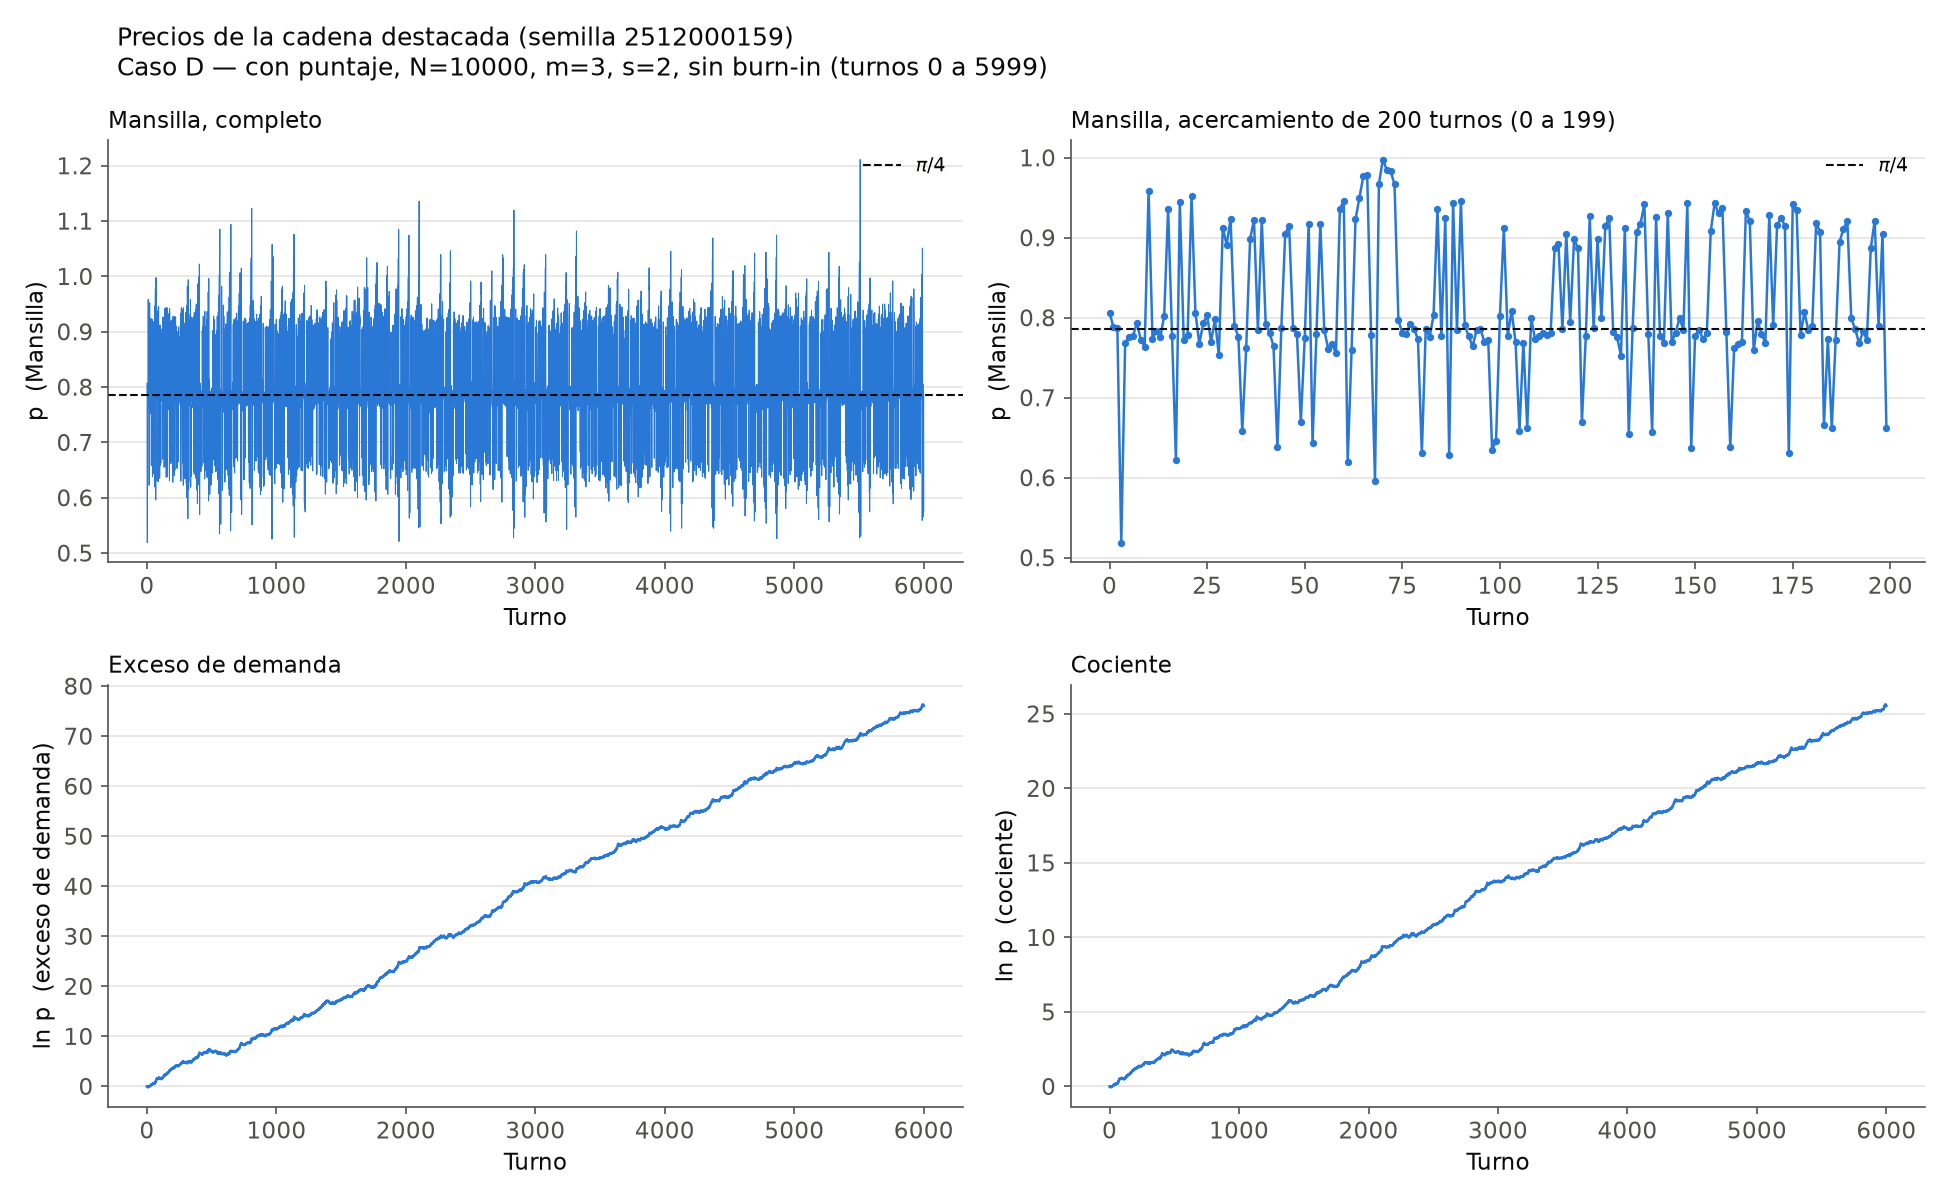
\includegraphics[width=0.49\textwidth]{figuras/Fase9_precios_detalle_casoD_N10000_m3_s2_con_puntaje_T6000_regla_nueva_sin_burnin.png}\hfill
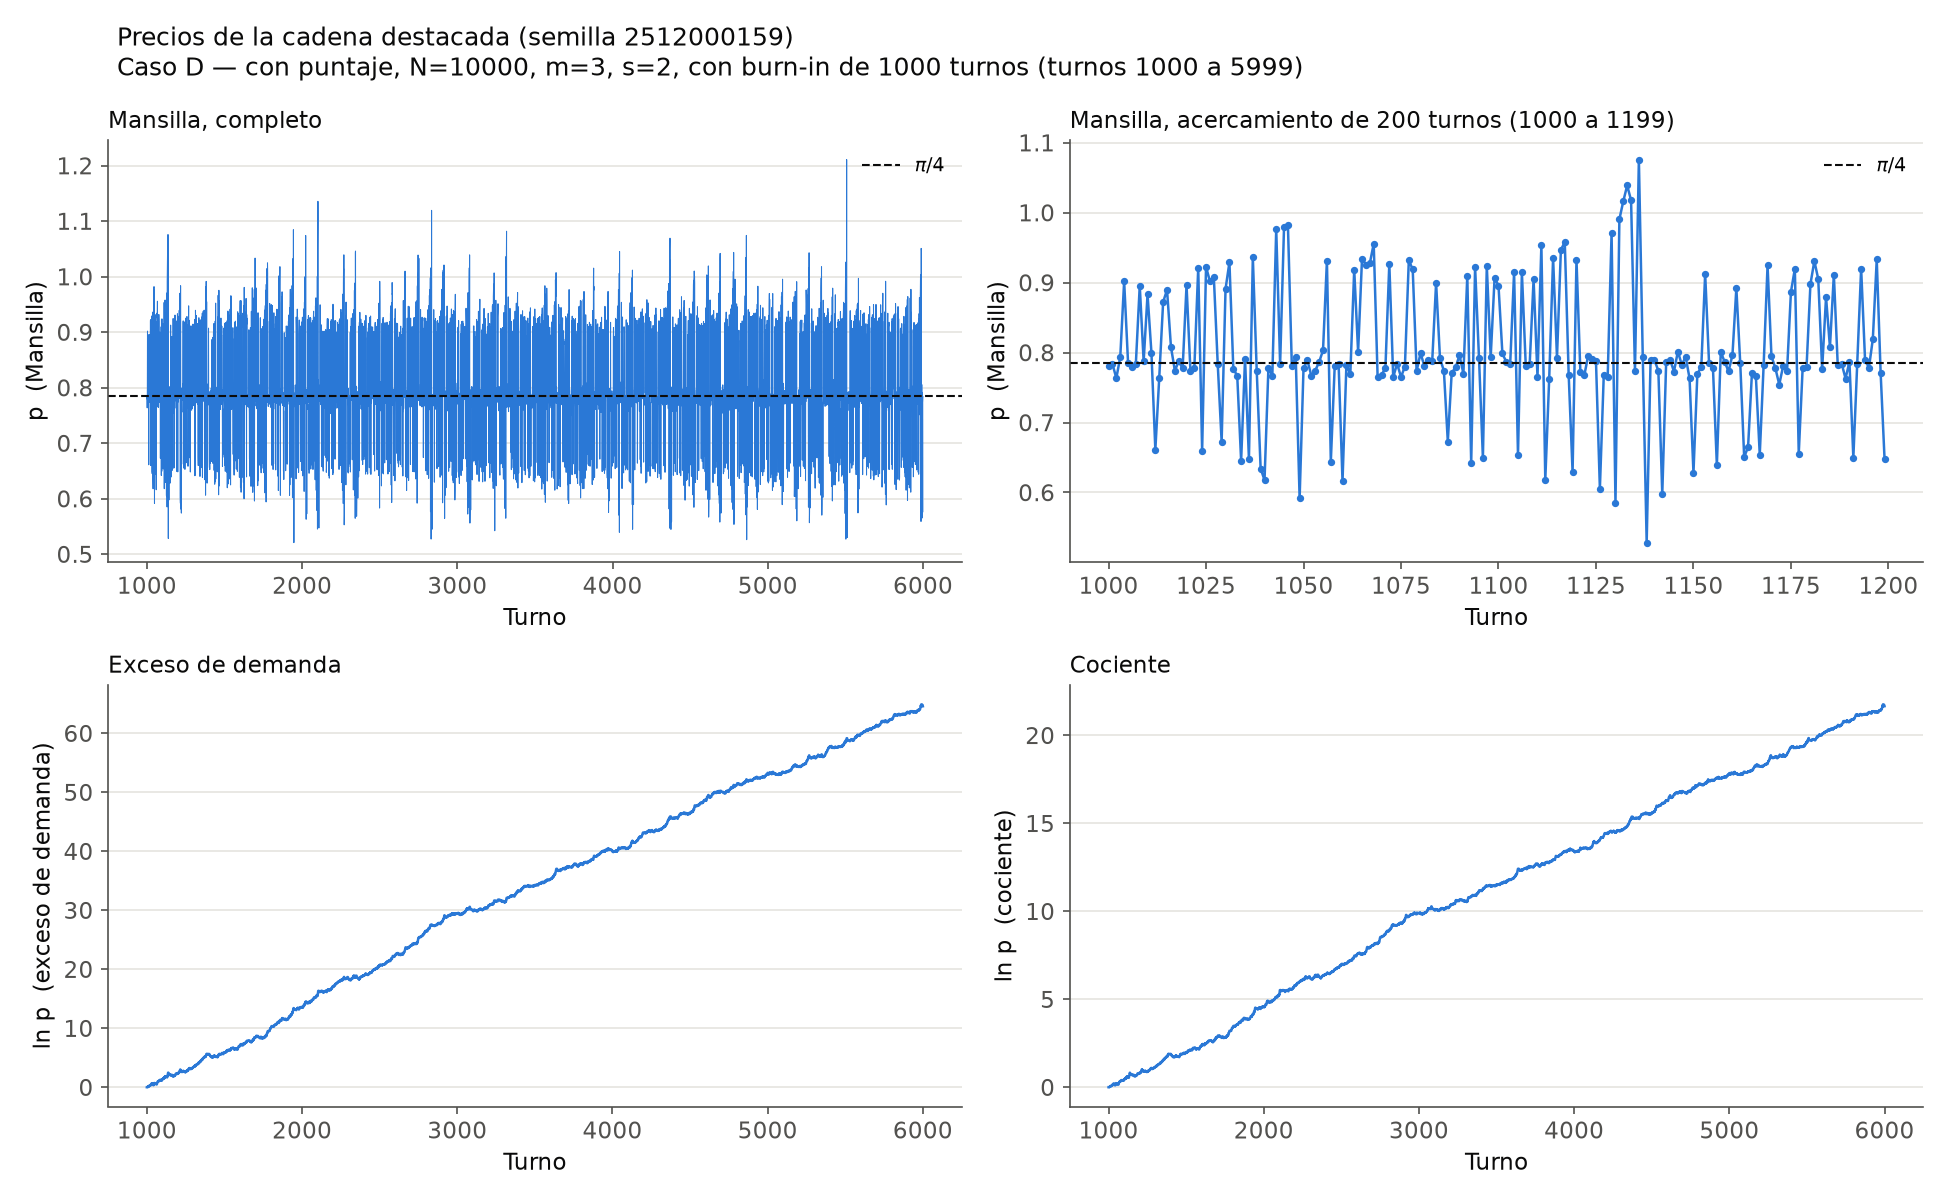
\includegraphics[width=0.49\textwidth]{figuras/Fase9_precios_detalle_casoD_N10000_m3_s2_con_puntaje_T6000_regla_nueva_con_burnin1000.png}
\caption{Caso D, $N=10000$: detalle de la cadena destacada sin burn-in (izquierda) y con burn-in (derecha).}
\end{figure}

\begin{figure}[H]
\centering
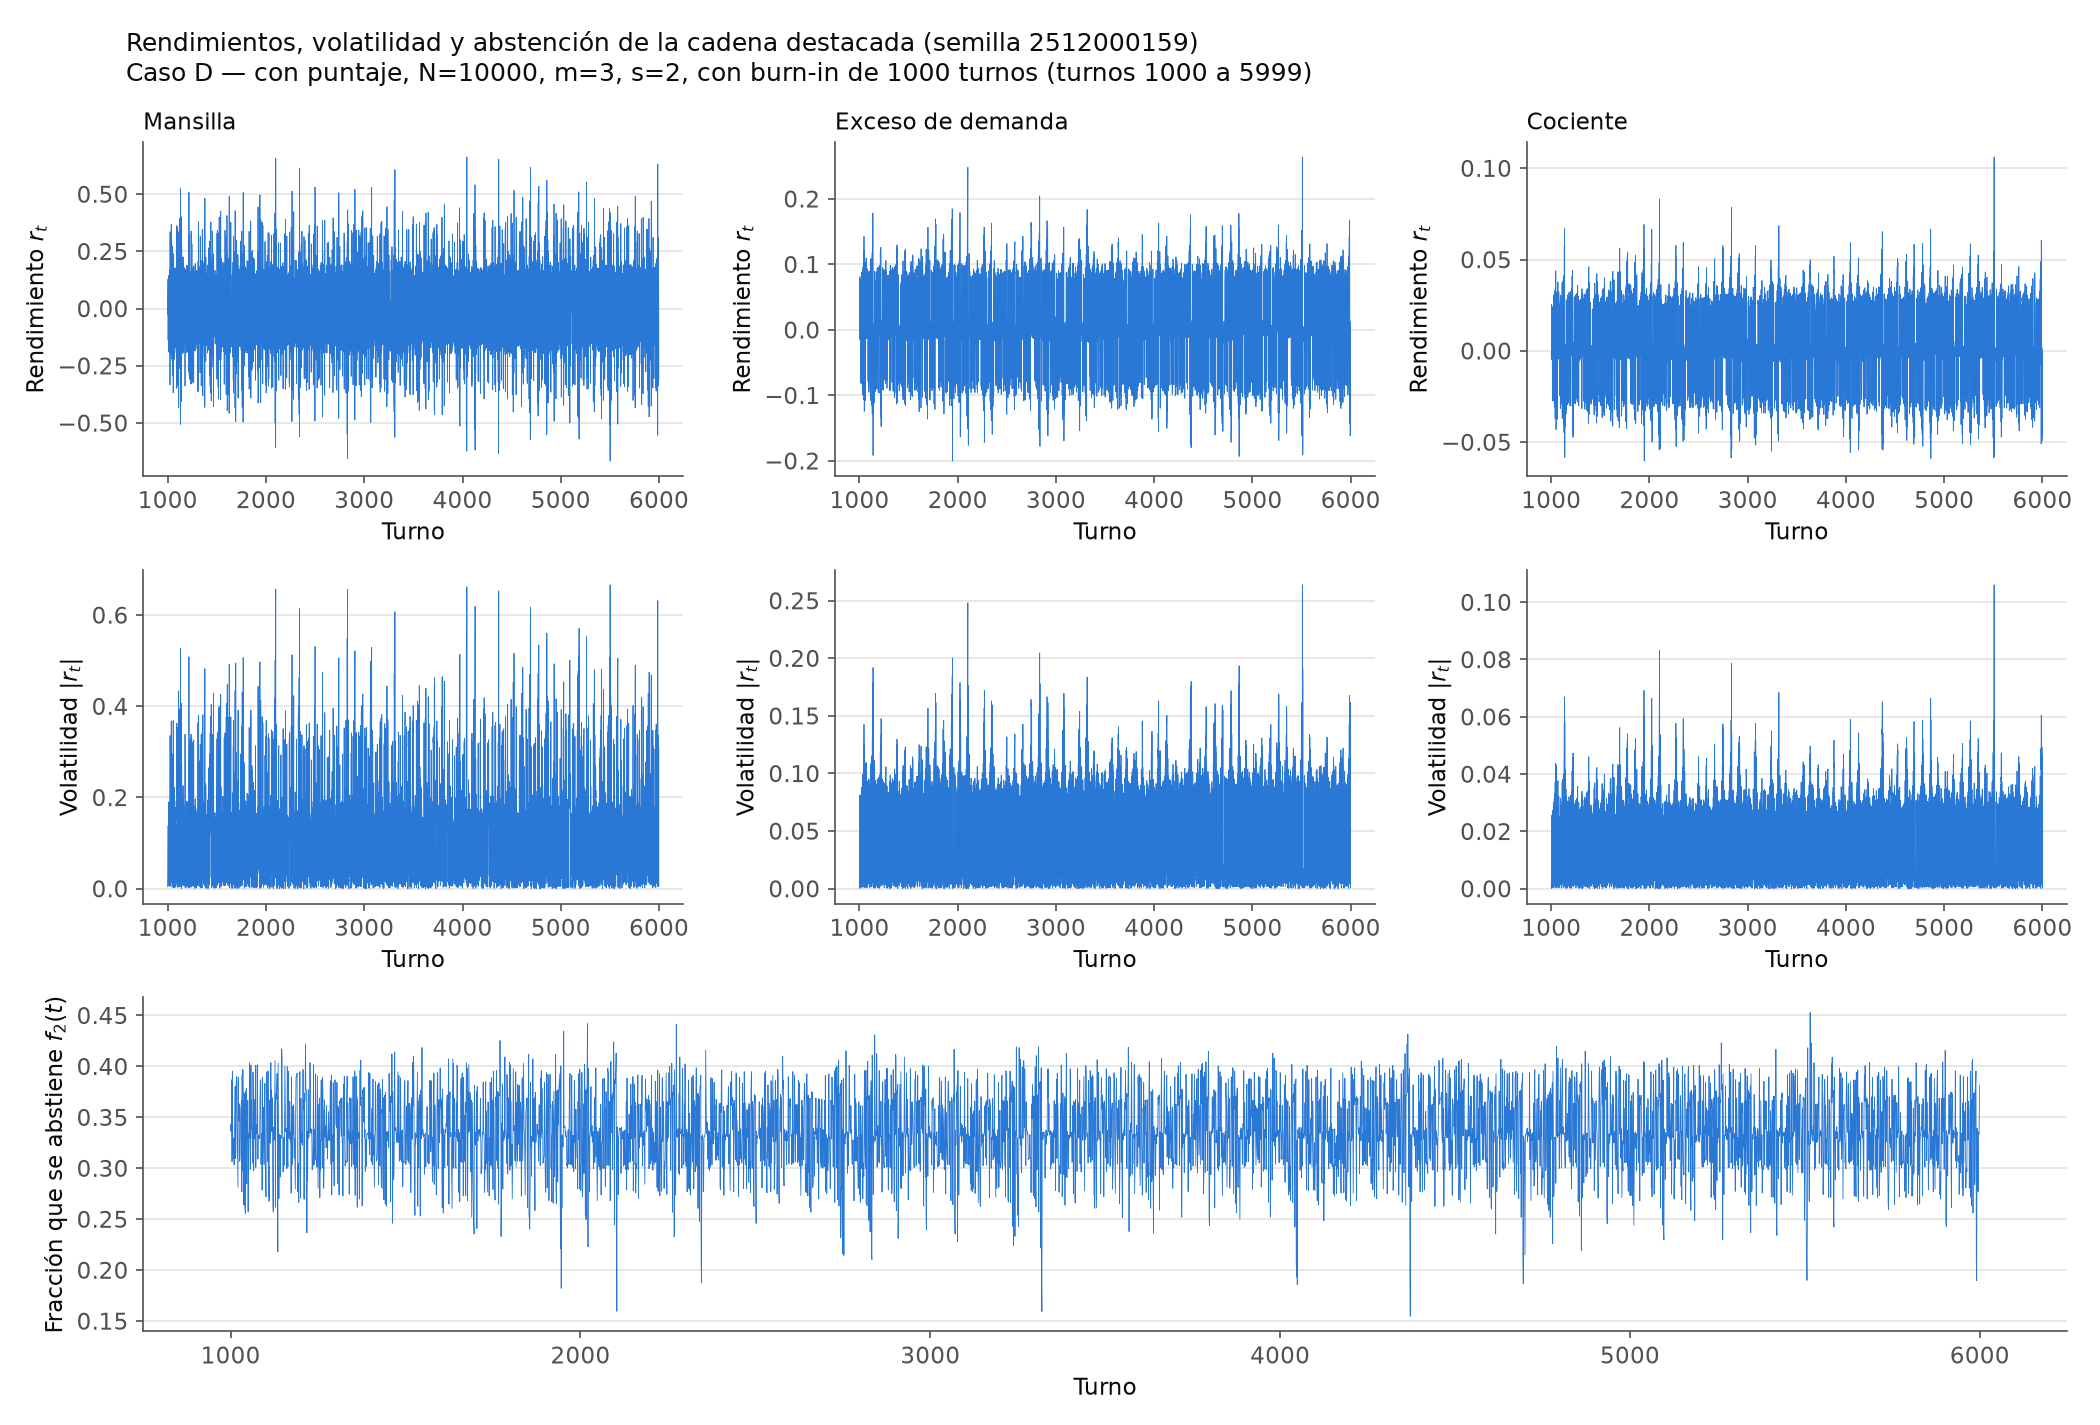
\includegraphics[width=0.85\textwidth]{figuras/Fase9_series_casoD_N10000_m3_s2_con_puntaje_T6000_regla_nueva_con_burnin1000.png}
\caption{Caso D: rendimientos, volatilidad y fracción que se abstiene de la cadena destacada, con burn-in.}
\end{figure}

\begin{figure}[H]
\centering
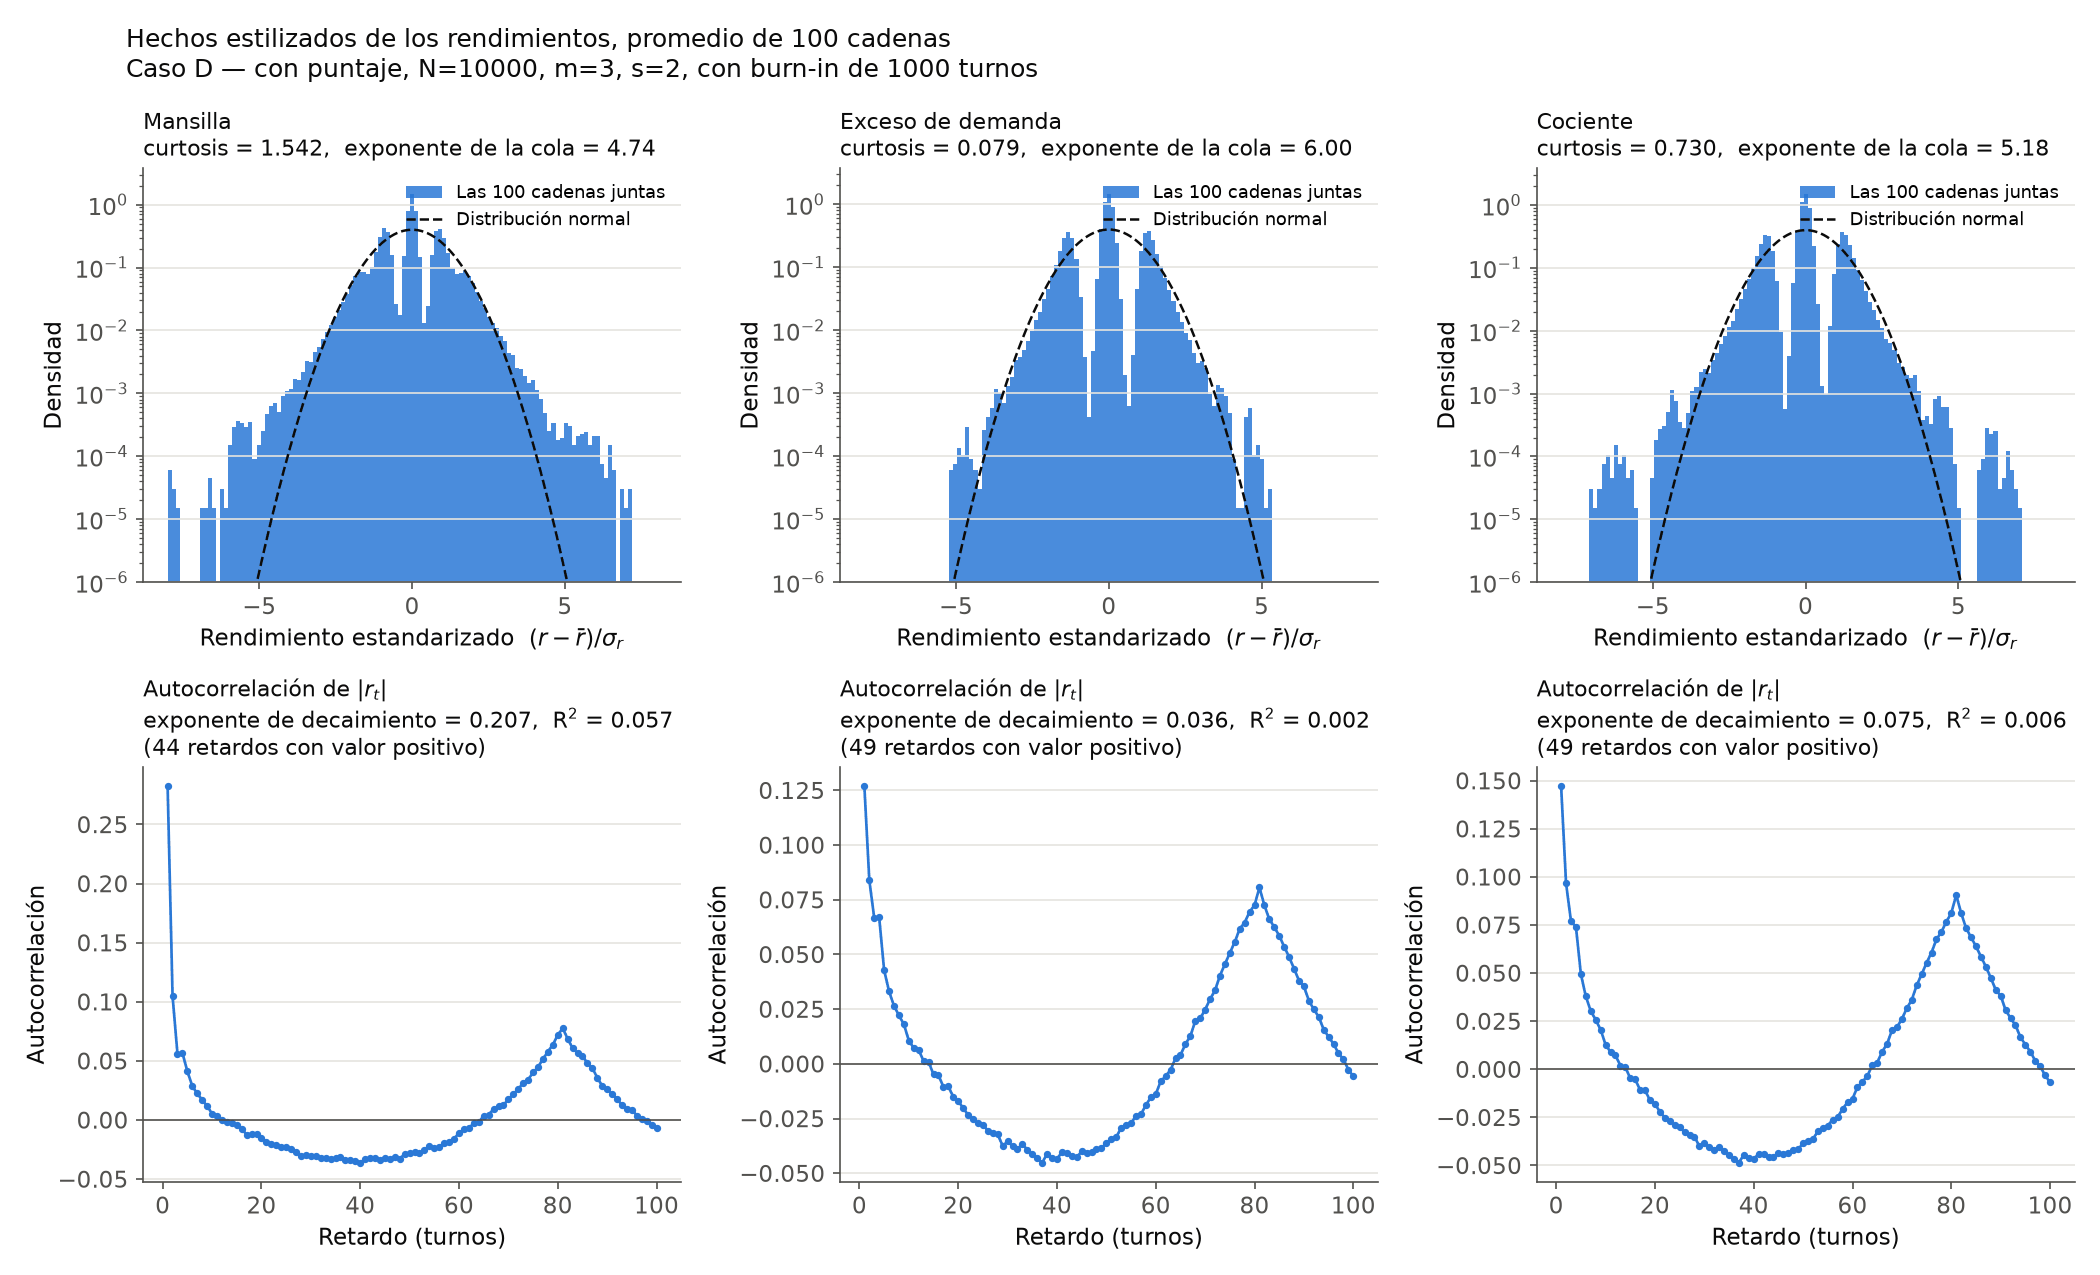
\includegraphics[width=0.85\textwidth]{figuras/Fase9_hechos_estilizados_casoD_N10000_m3_s2_con_puntaje_T6000_regla_nueva_con_burnin1000.png}
\caption{Caso D: hechos estilizados (distribución de los rendimientos y autocorrelación de $|r|$), con burn-in.}
\end{figure}

\begin{figure}[H]
\centering
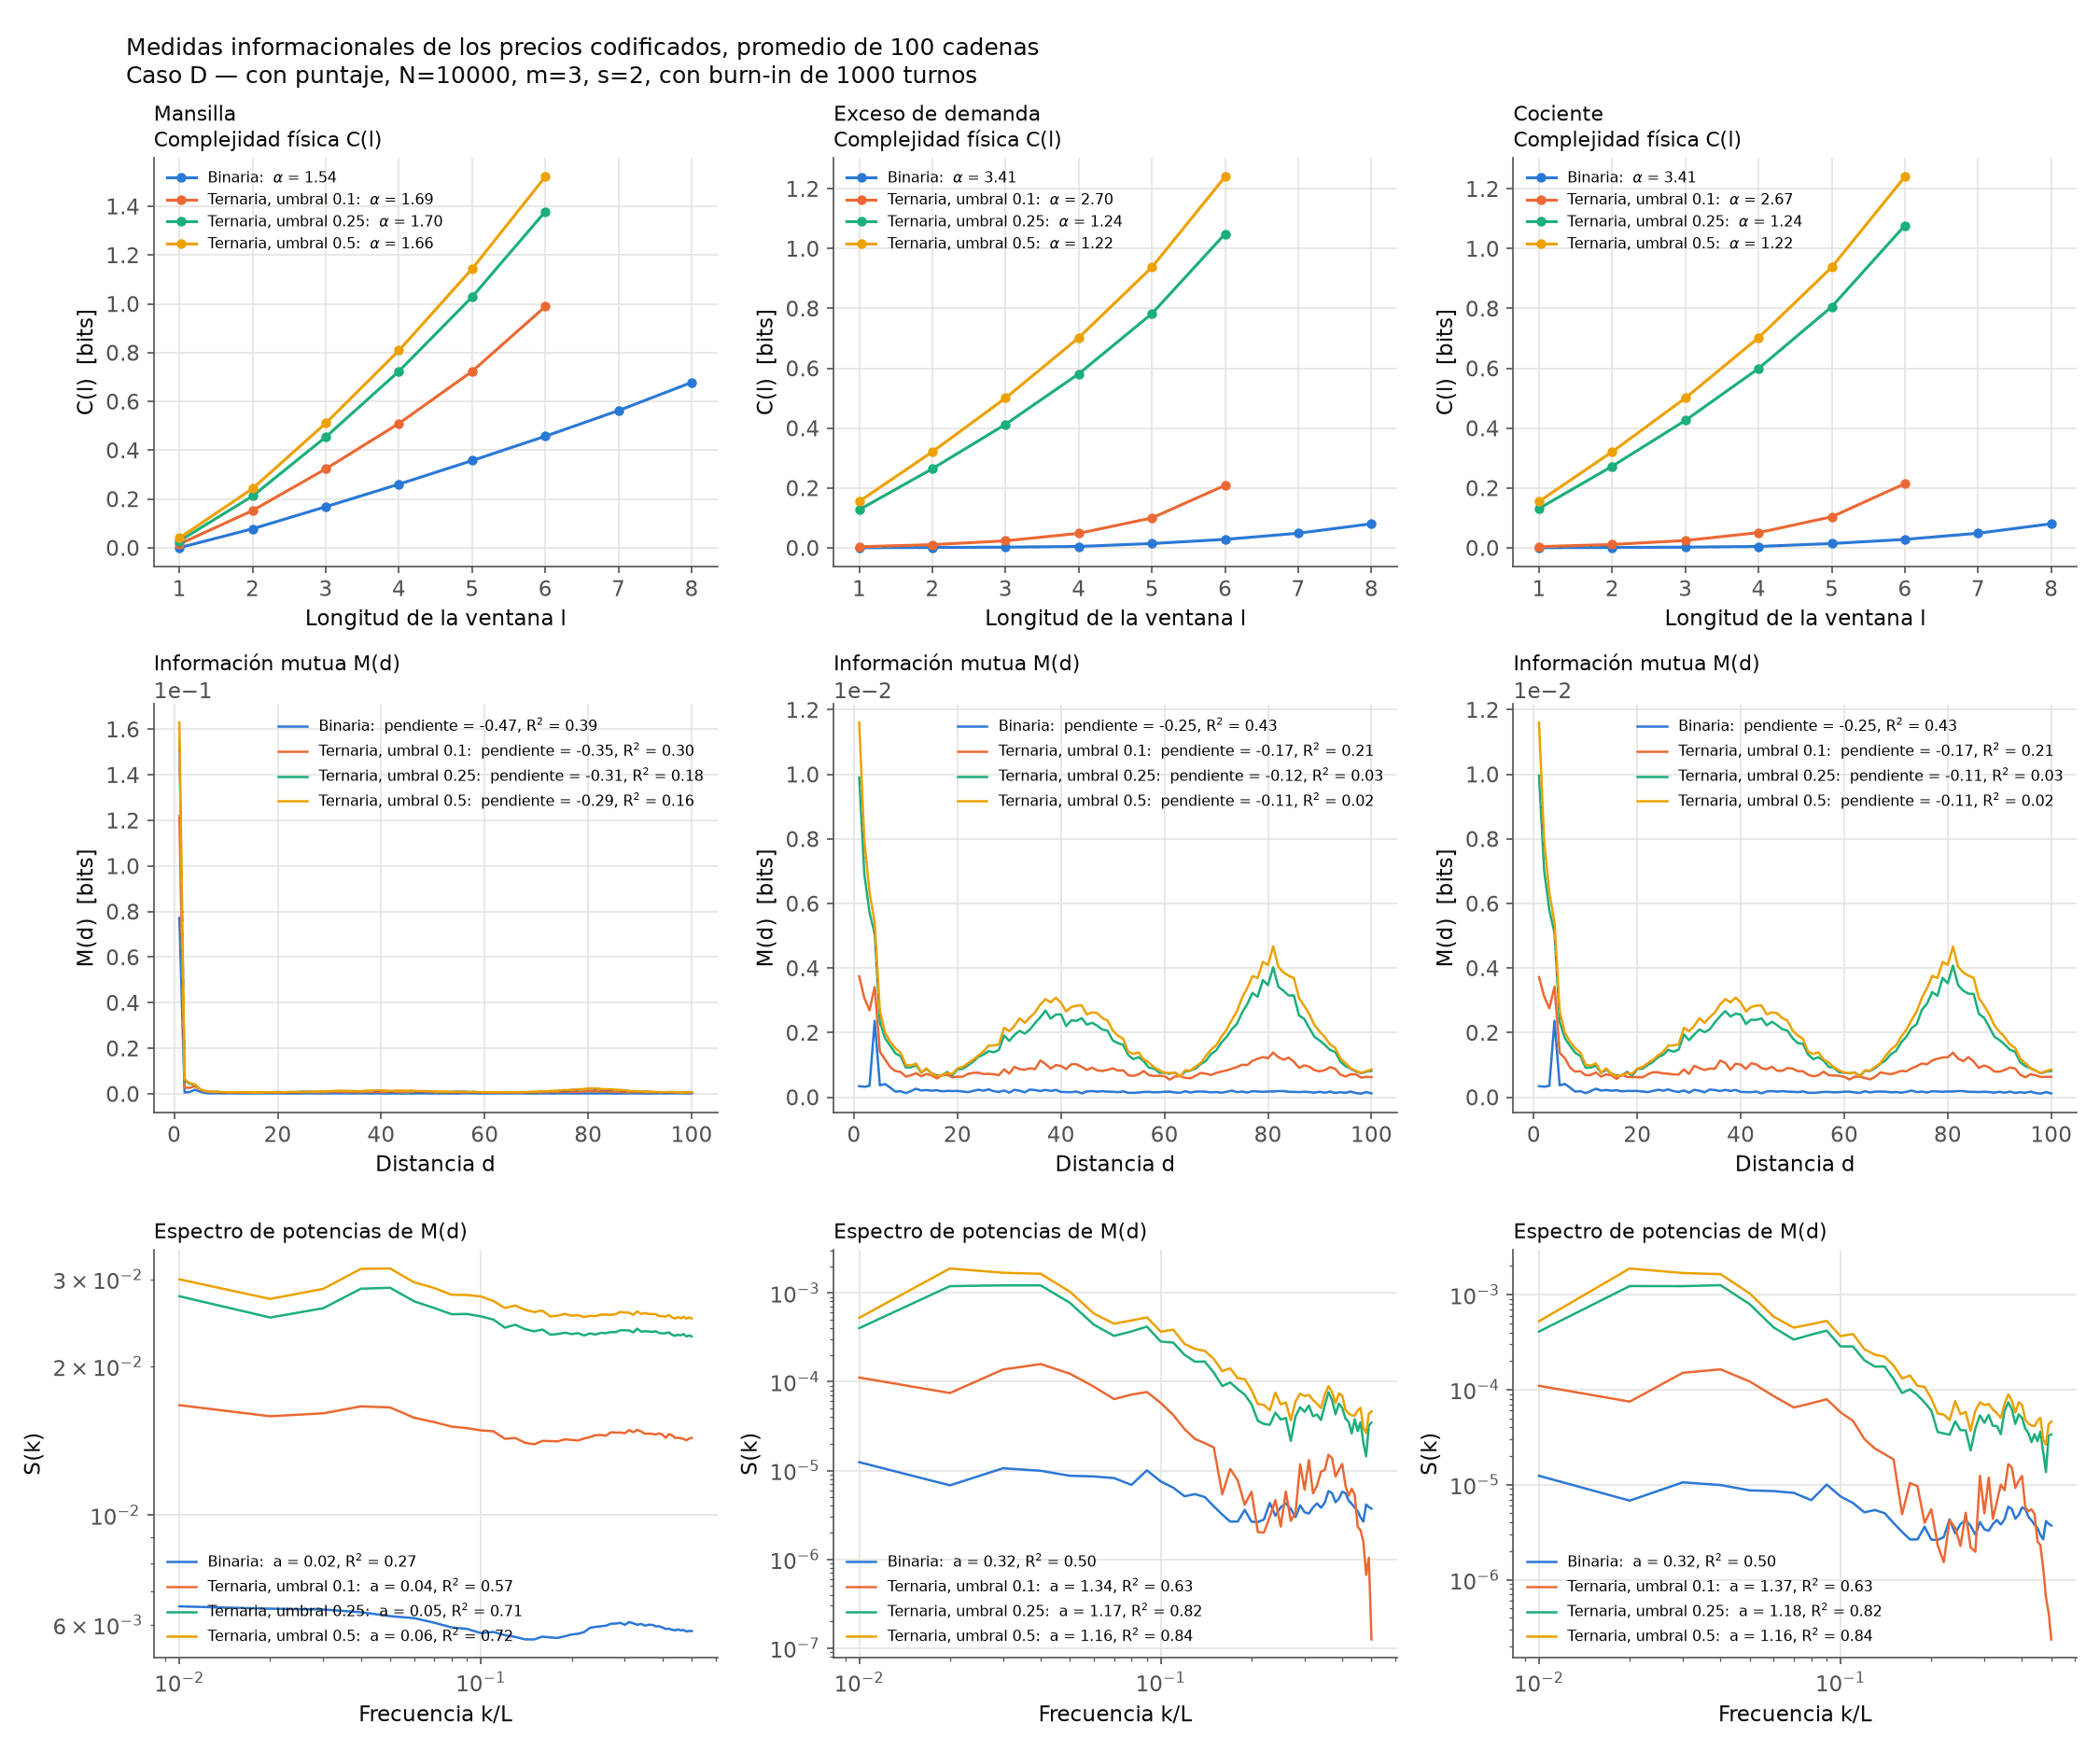
\includegraphics[width=0.85\textwidth]{figuras/Fase9_medidas_informacionales_casoD_N10000_m3_s2_con_puntaje_T6000_regla_nueva_con_burnin1000.png}
\caption{Caso D: medidas informacionales de los precios codificados, con burn-in.}
\end{figure}

\clearpage
\subsection{Caso E: $m=4$, con puntaje}
\begin{figure}[H]
\centering
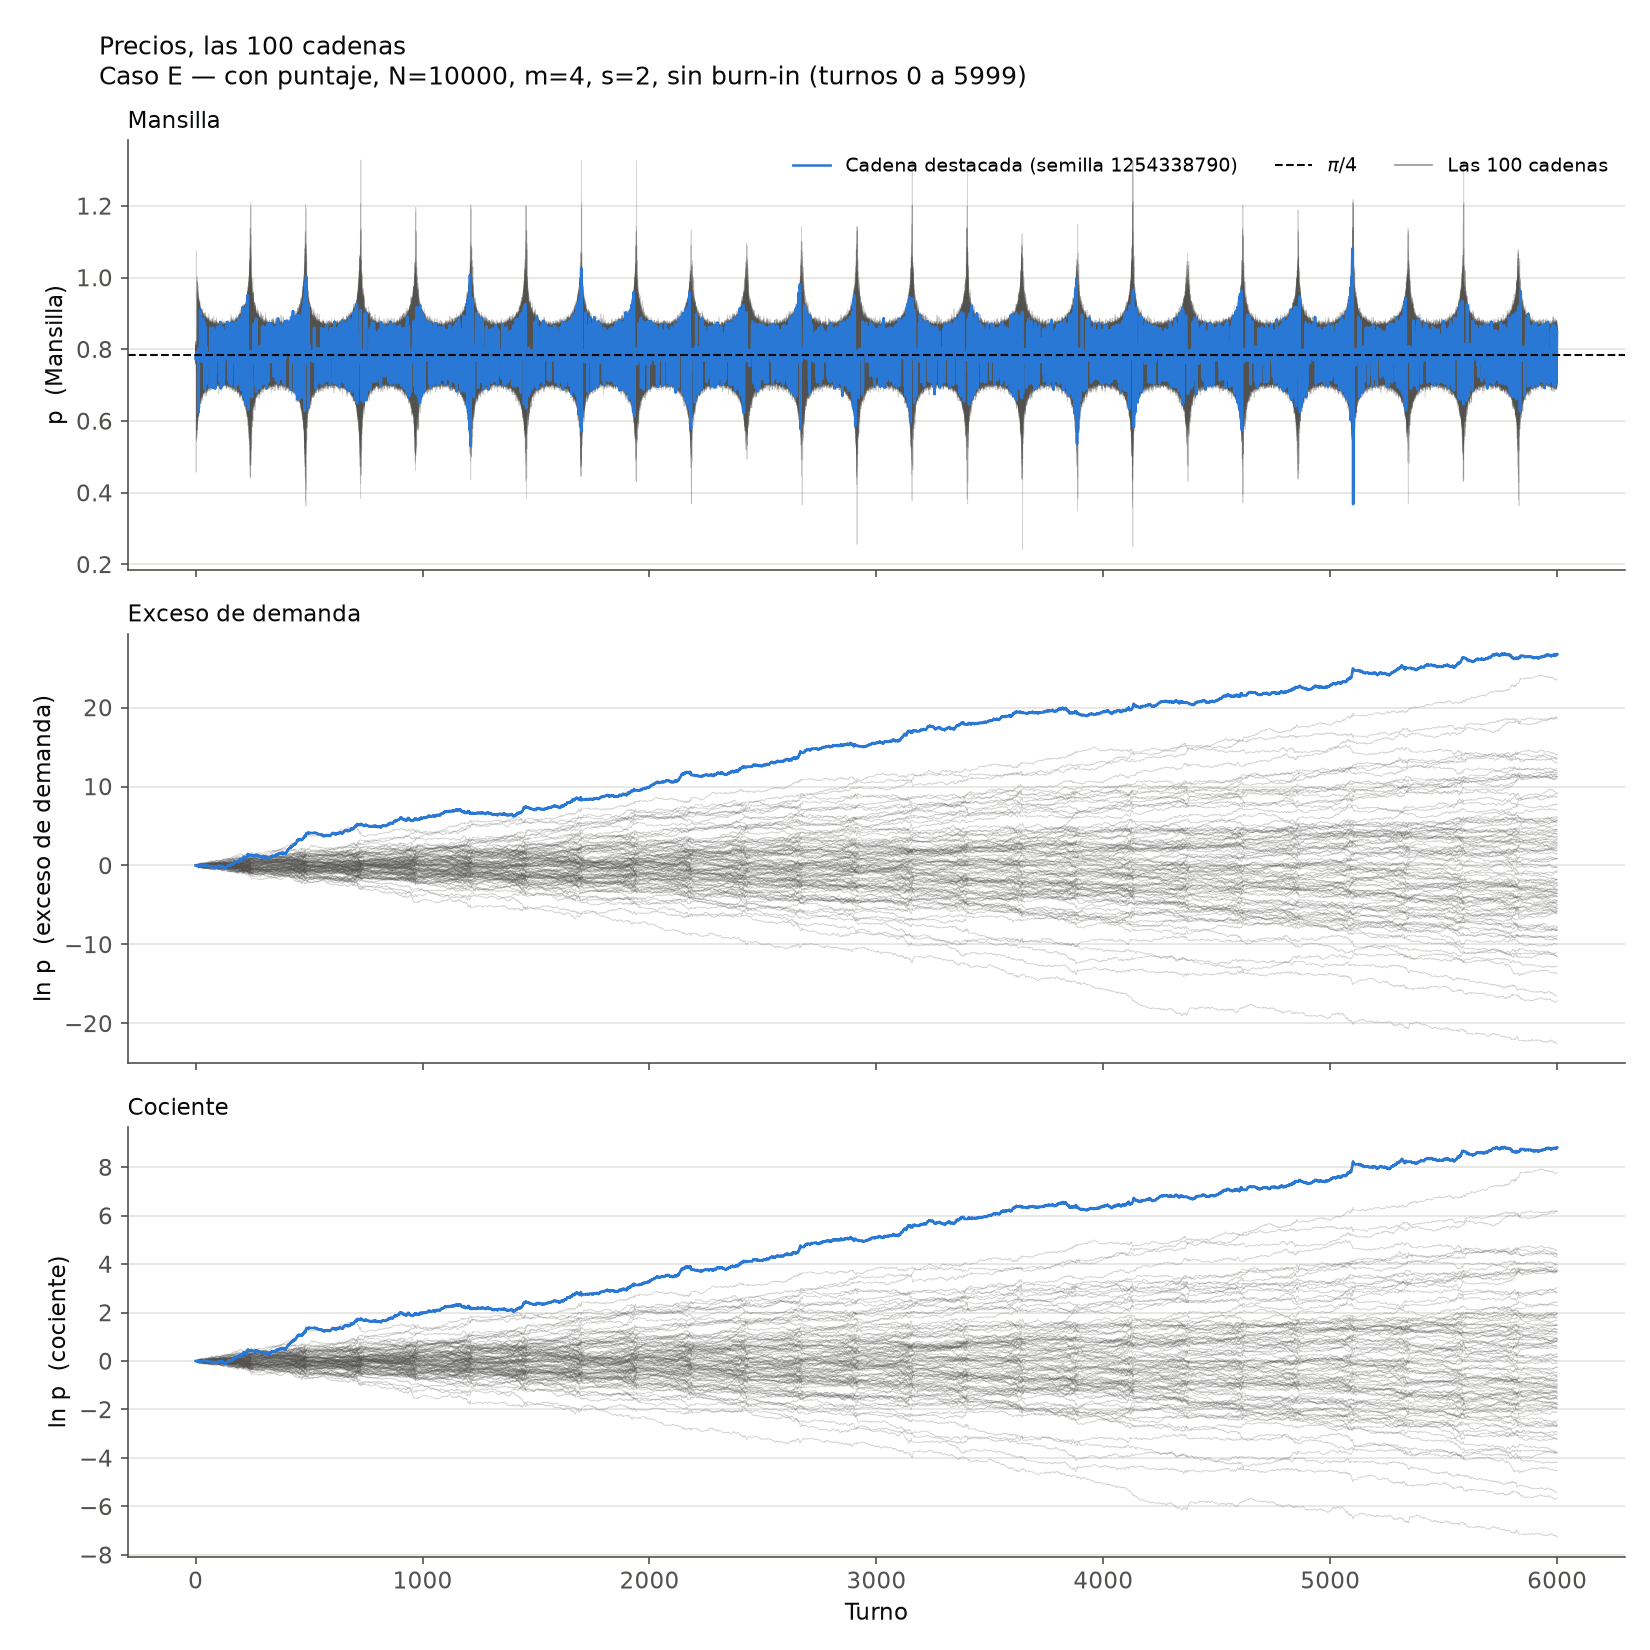
\includegraphics[width=0.49\textwidth]{figuras/Fase9_precios_conjunto_casoE_N10000_m4_s2_con_puntaje_T6000_regla_nueva_sin_burnin.png}\hfill
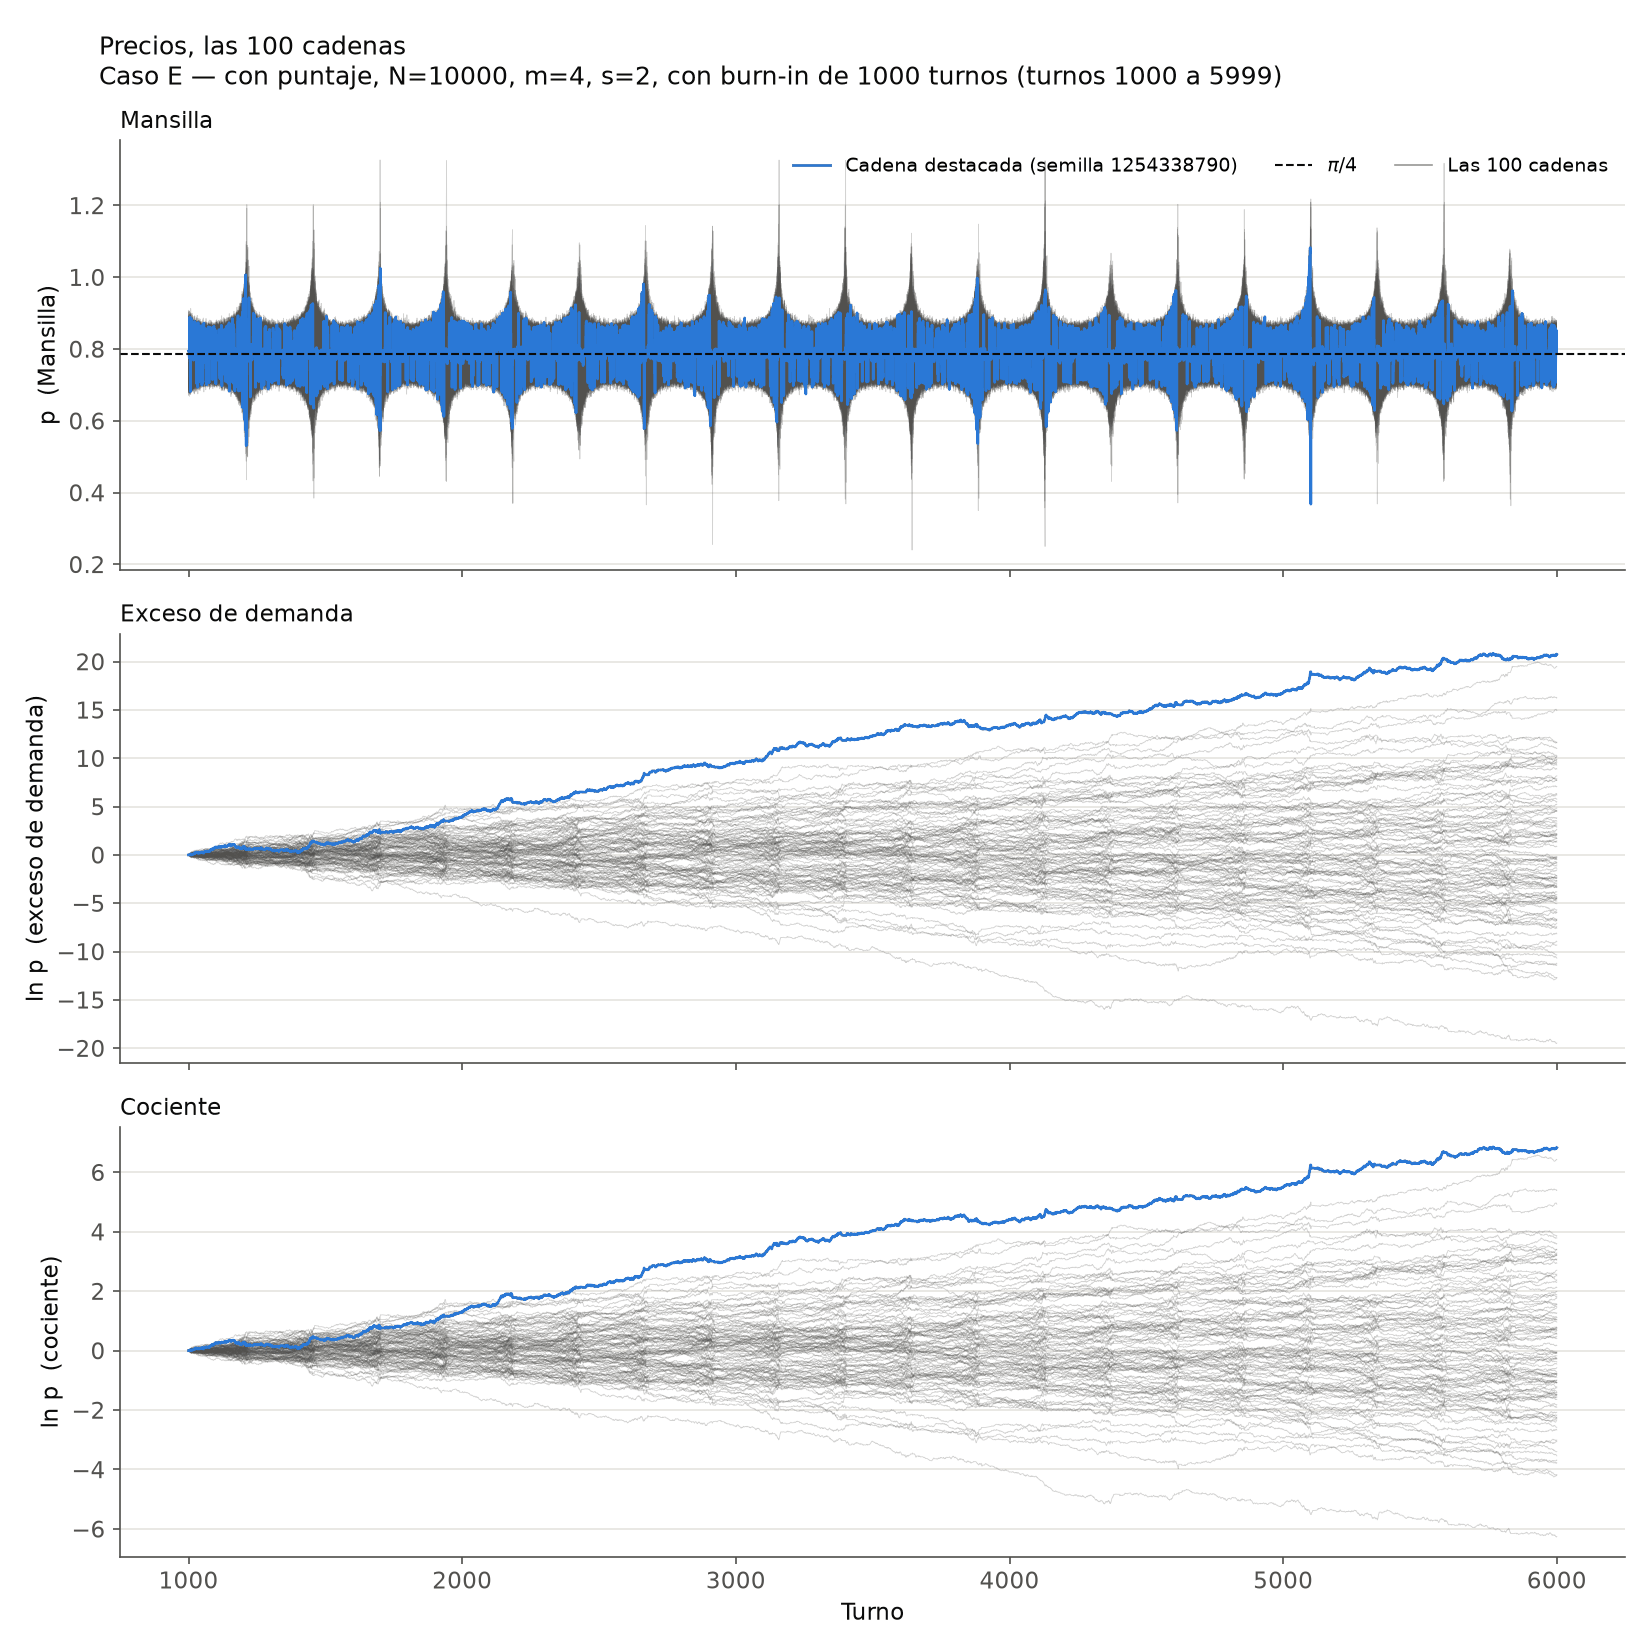
\includegraphics[width=0.49\textwidth]{figuras/Fase9_precios_conjunto_casoE_N10000_m4_s2_con_puntaje_T6000_regla_nueva_con_burnin1000.png}
\caption{Caso E, $N=10000$: conjunto de precios sin burn-in (izquierda) y con burn-in (derecha).}
\end{figure}

\begin{figure}[H]
\centering
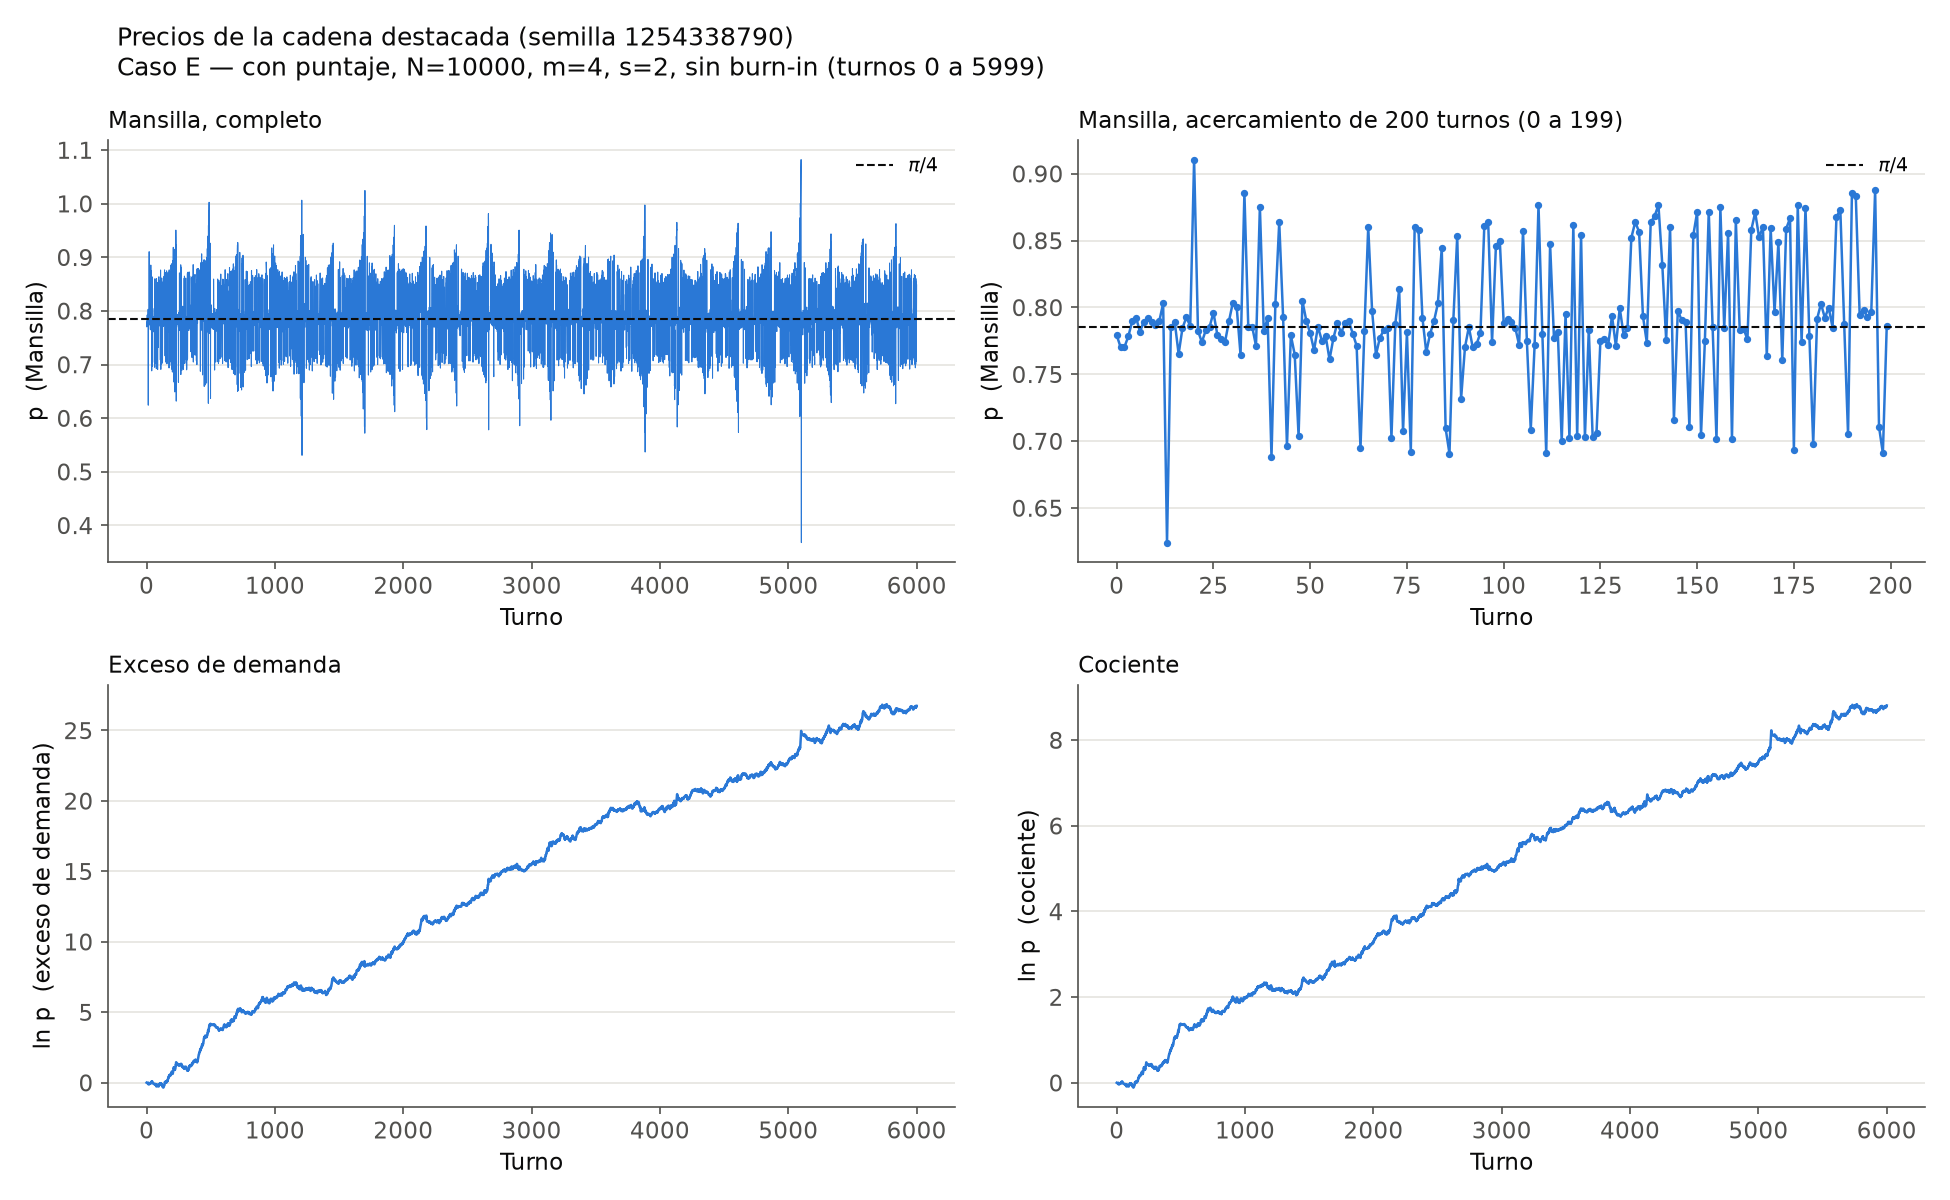
\includegraphics[width=0.49\textwidth]{figuras/Fase9_precios_detalle_casoE_N10000_m4_s2_con_puntaje_T6000_regla_nueva_sin_burnin.png}\hfill
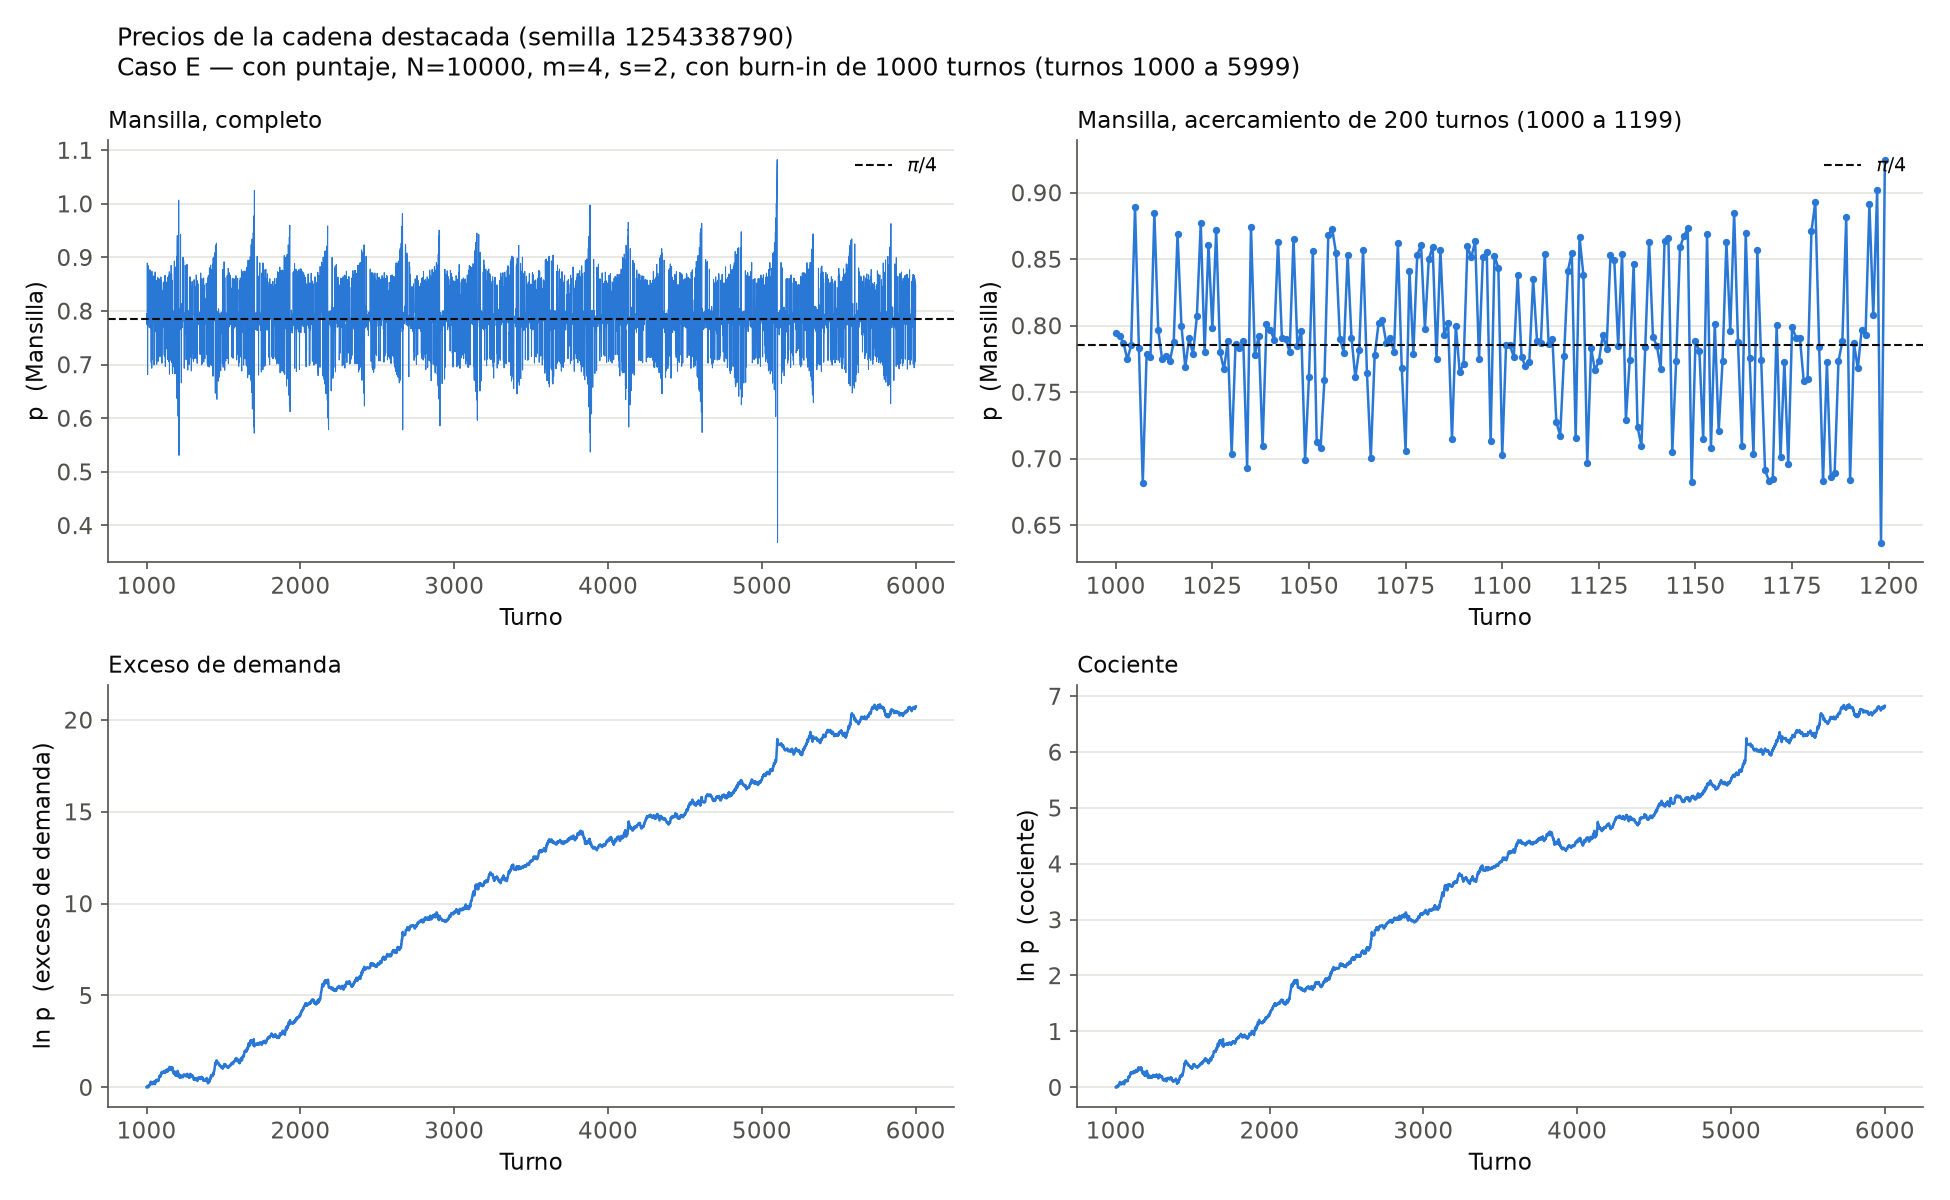
\includegraphics[width=0.49\textwidth]{figuras/Fase9_precios_detalle_casoE_N10000_m4_s2_con_puntaje_T6000_regla_nueva_con_burnin1000.png}
\caption{Caso E, $N=10000$: detalle de la cadena destacada sin burn-in (izquierda) y con burn-in (derecha).}
\end{figure}

\begin{figure}[H]
\centering
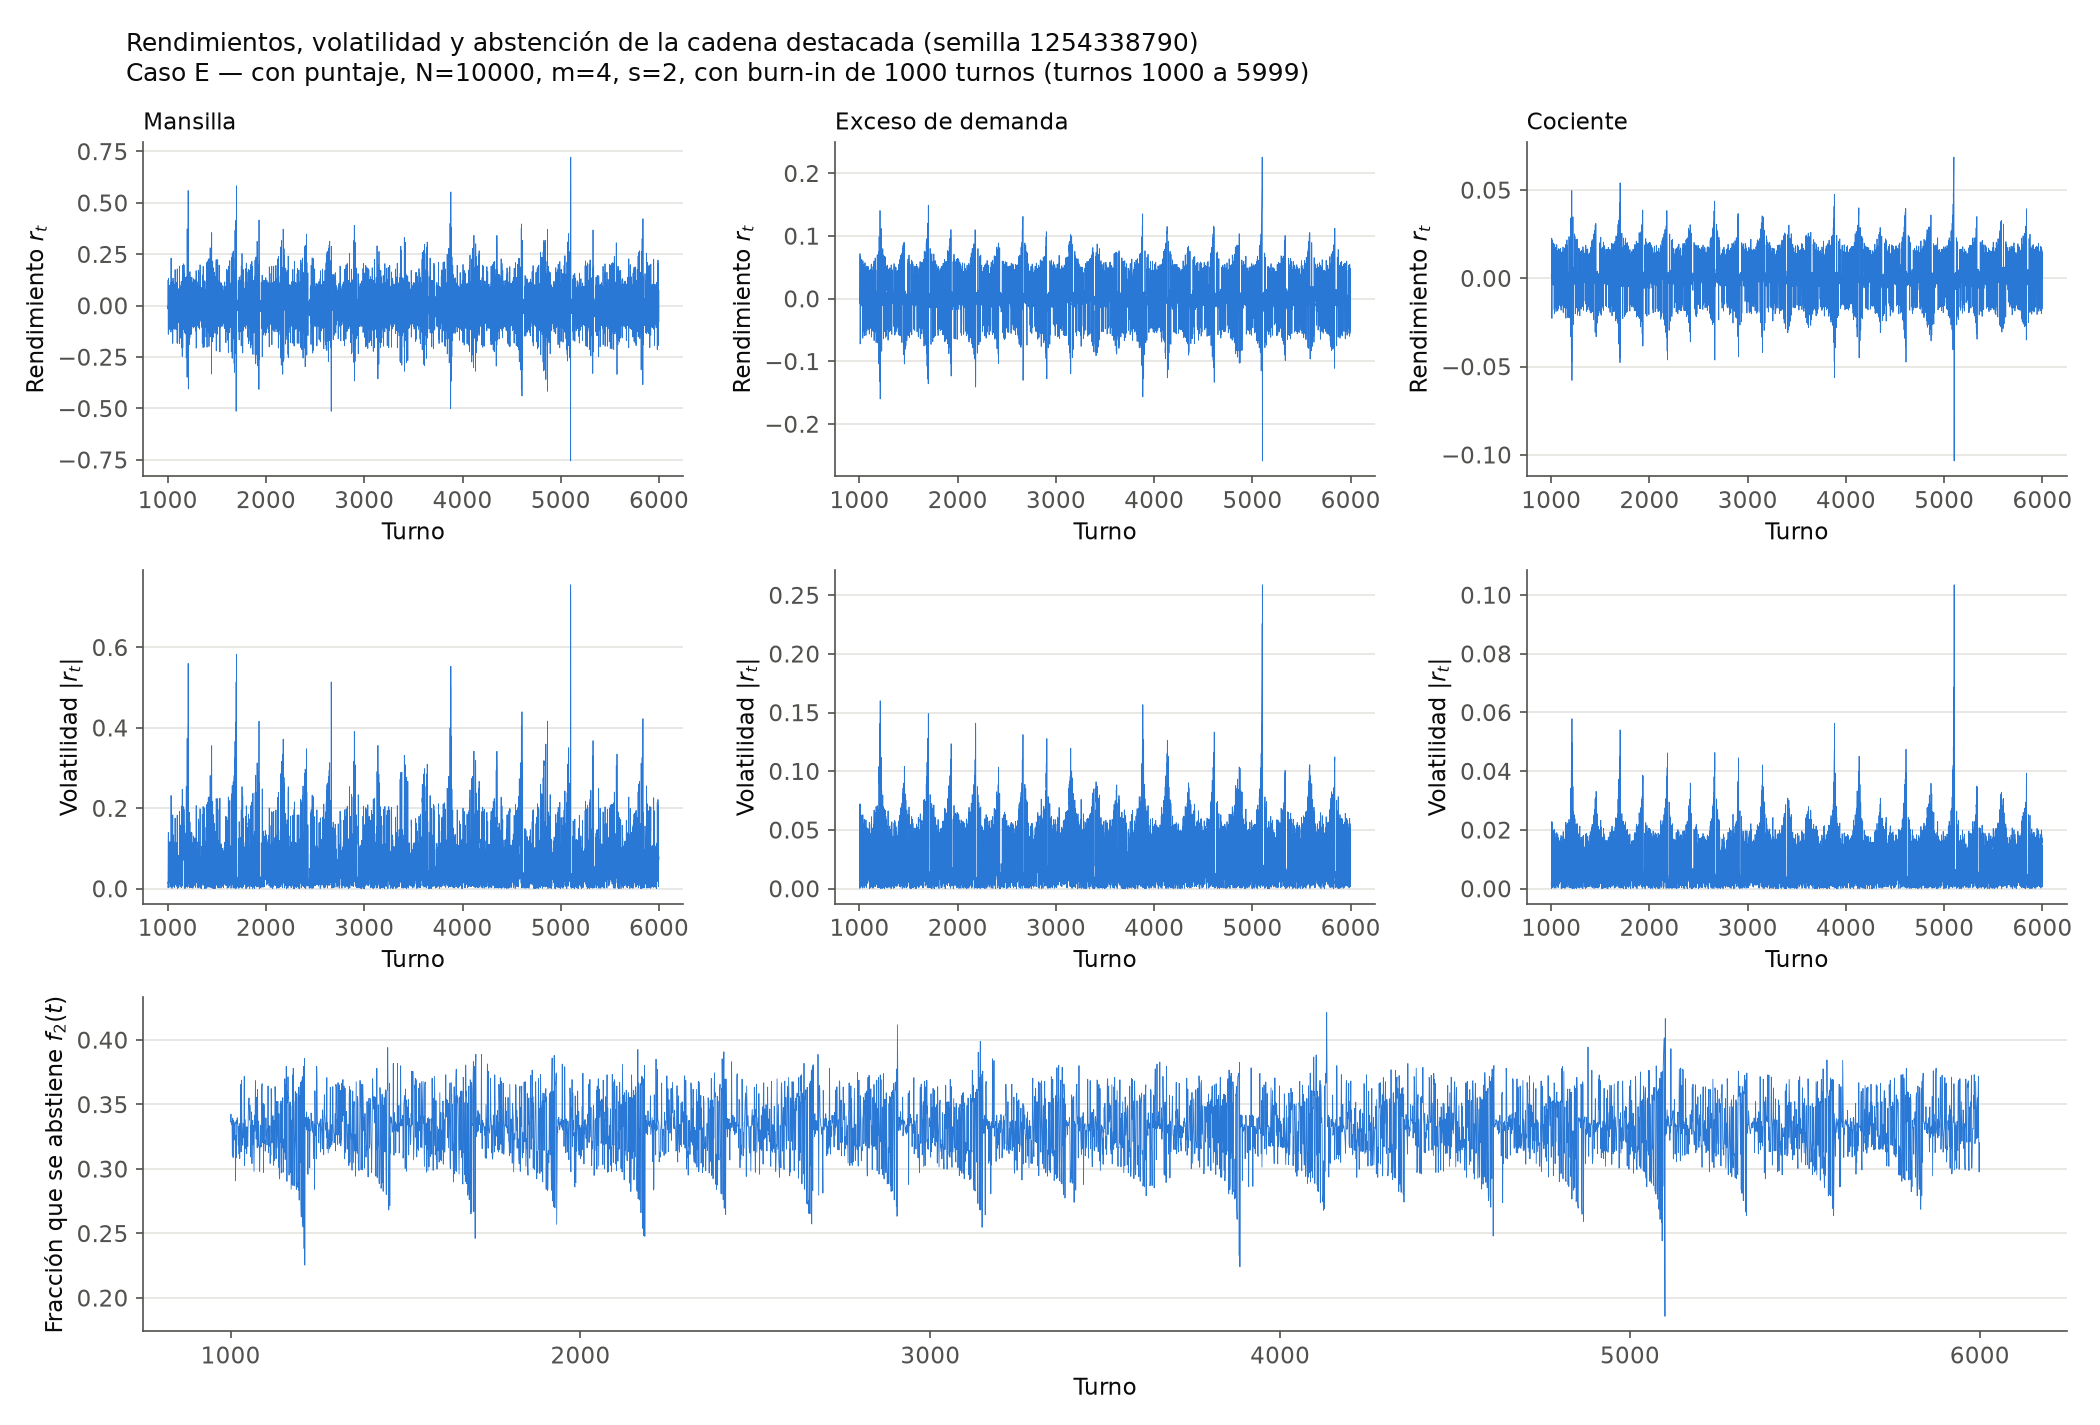
\includegraphics[width=0.85\textwidth]{figuras/Fase9_series_casoE_N10000_m4_s2_con_puntaje_T6000_regla_nueva_con_burnin1000.png}
\caption{Caso E: rendimientos, volatilidad y fracción que se abstiene de la cadena destacada, con burn-in.}
\end{figure}

\begin{figure}[H]
\centering
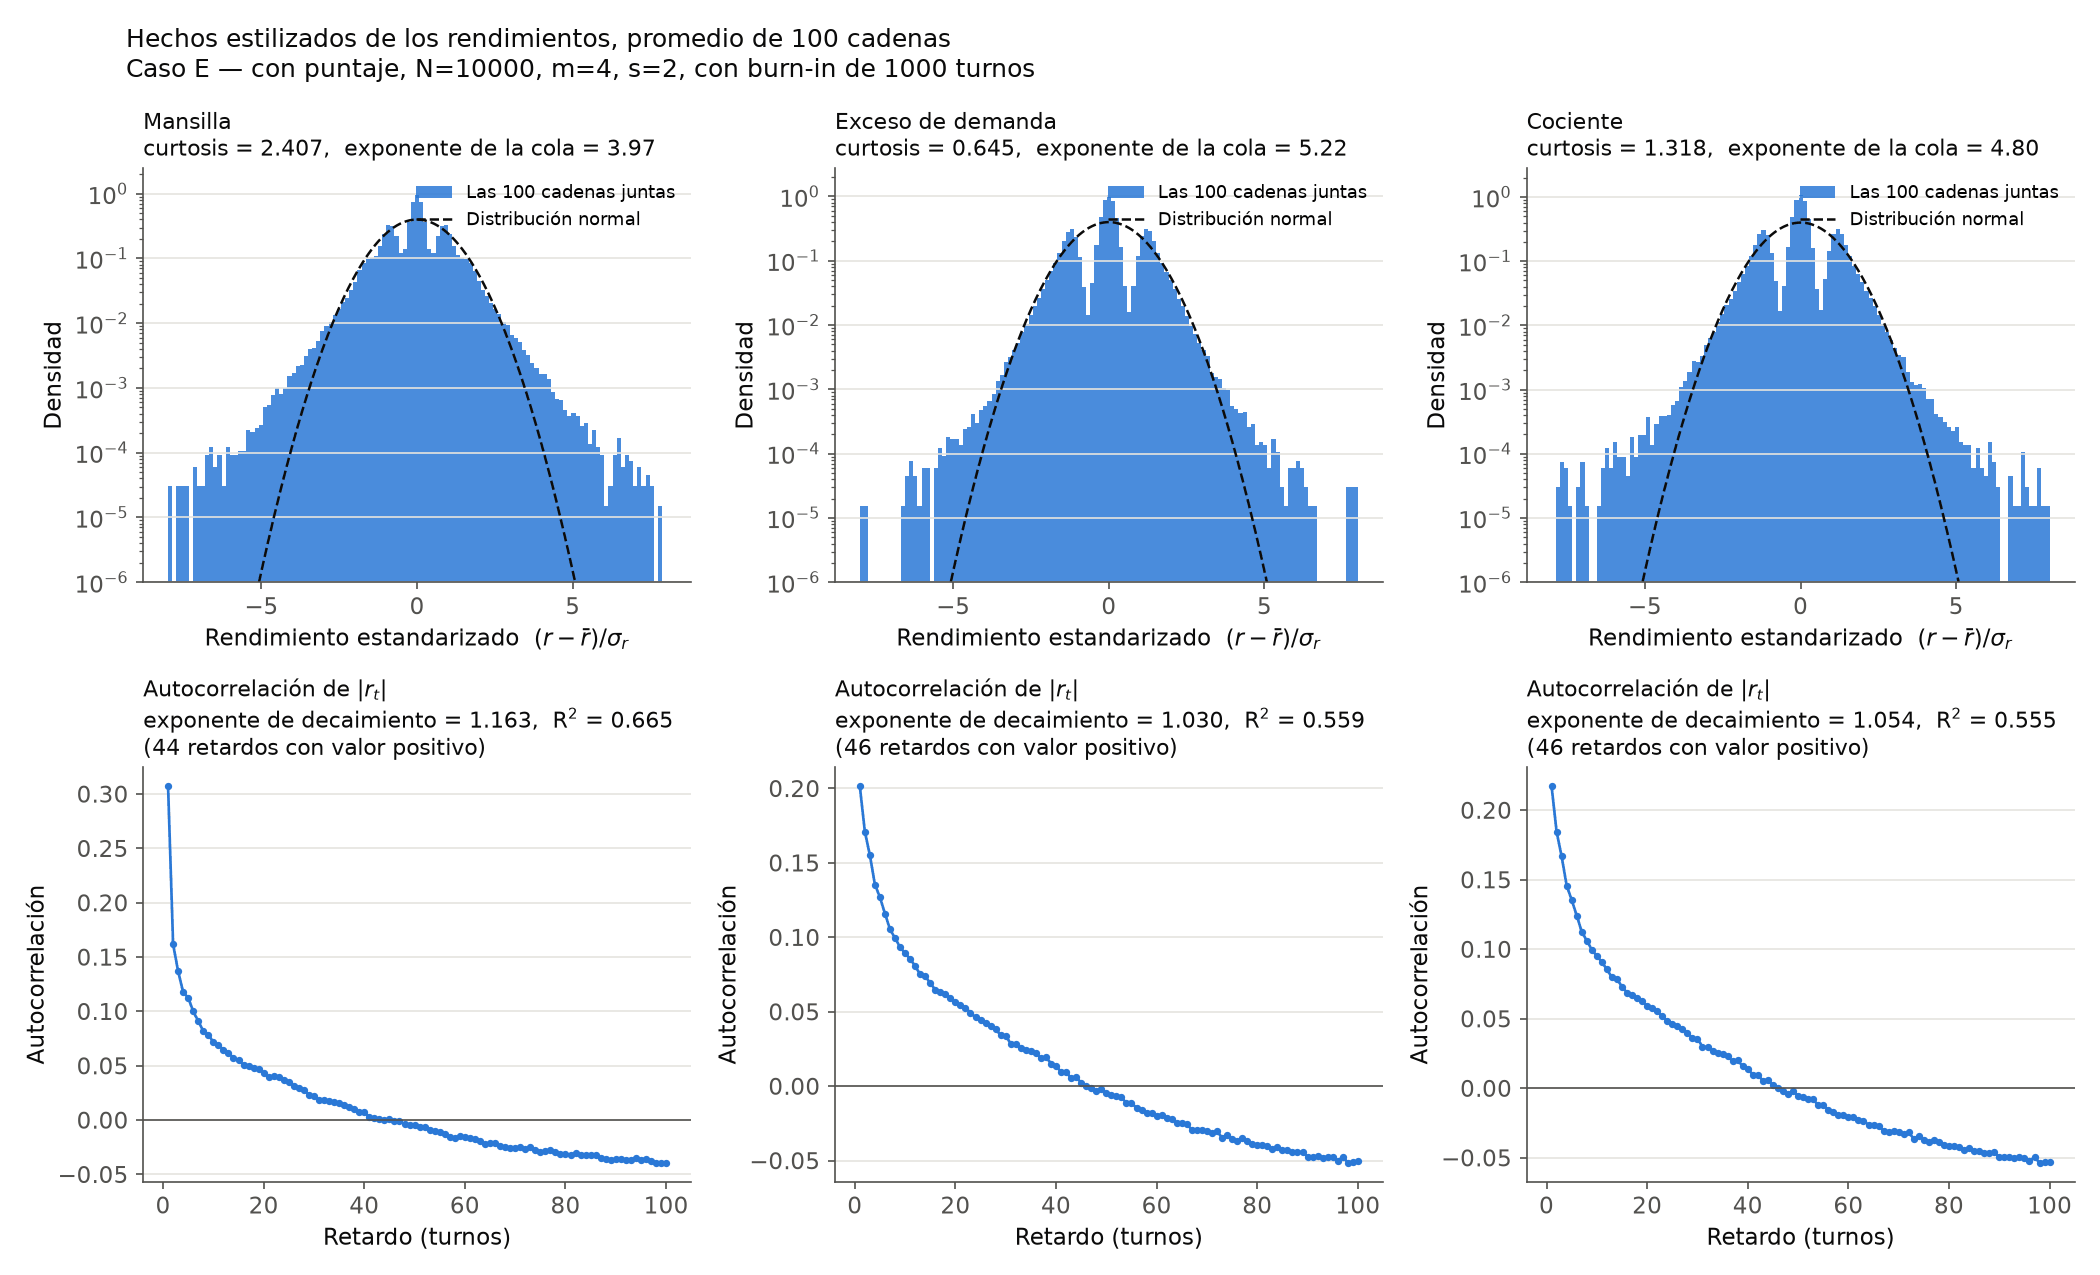
\includegraphics[width=0.85\textwidth]{figuras/Fase9_hechos_estilizados_casoE_N10000_m4_s2_con_puntaje_T6000_regla_nueva_con_burnin1000.png}
\caption{Caso E: hechos estilizados (distribución de los rendimientos y autocorrelación de $|r|$), con burn-in.}
\end{figure}

\begin{figure}[H]
\centering
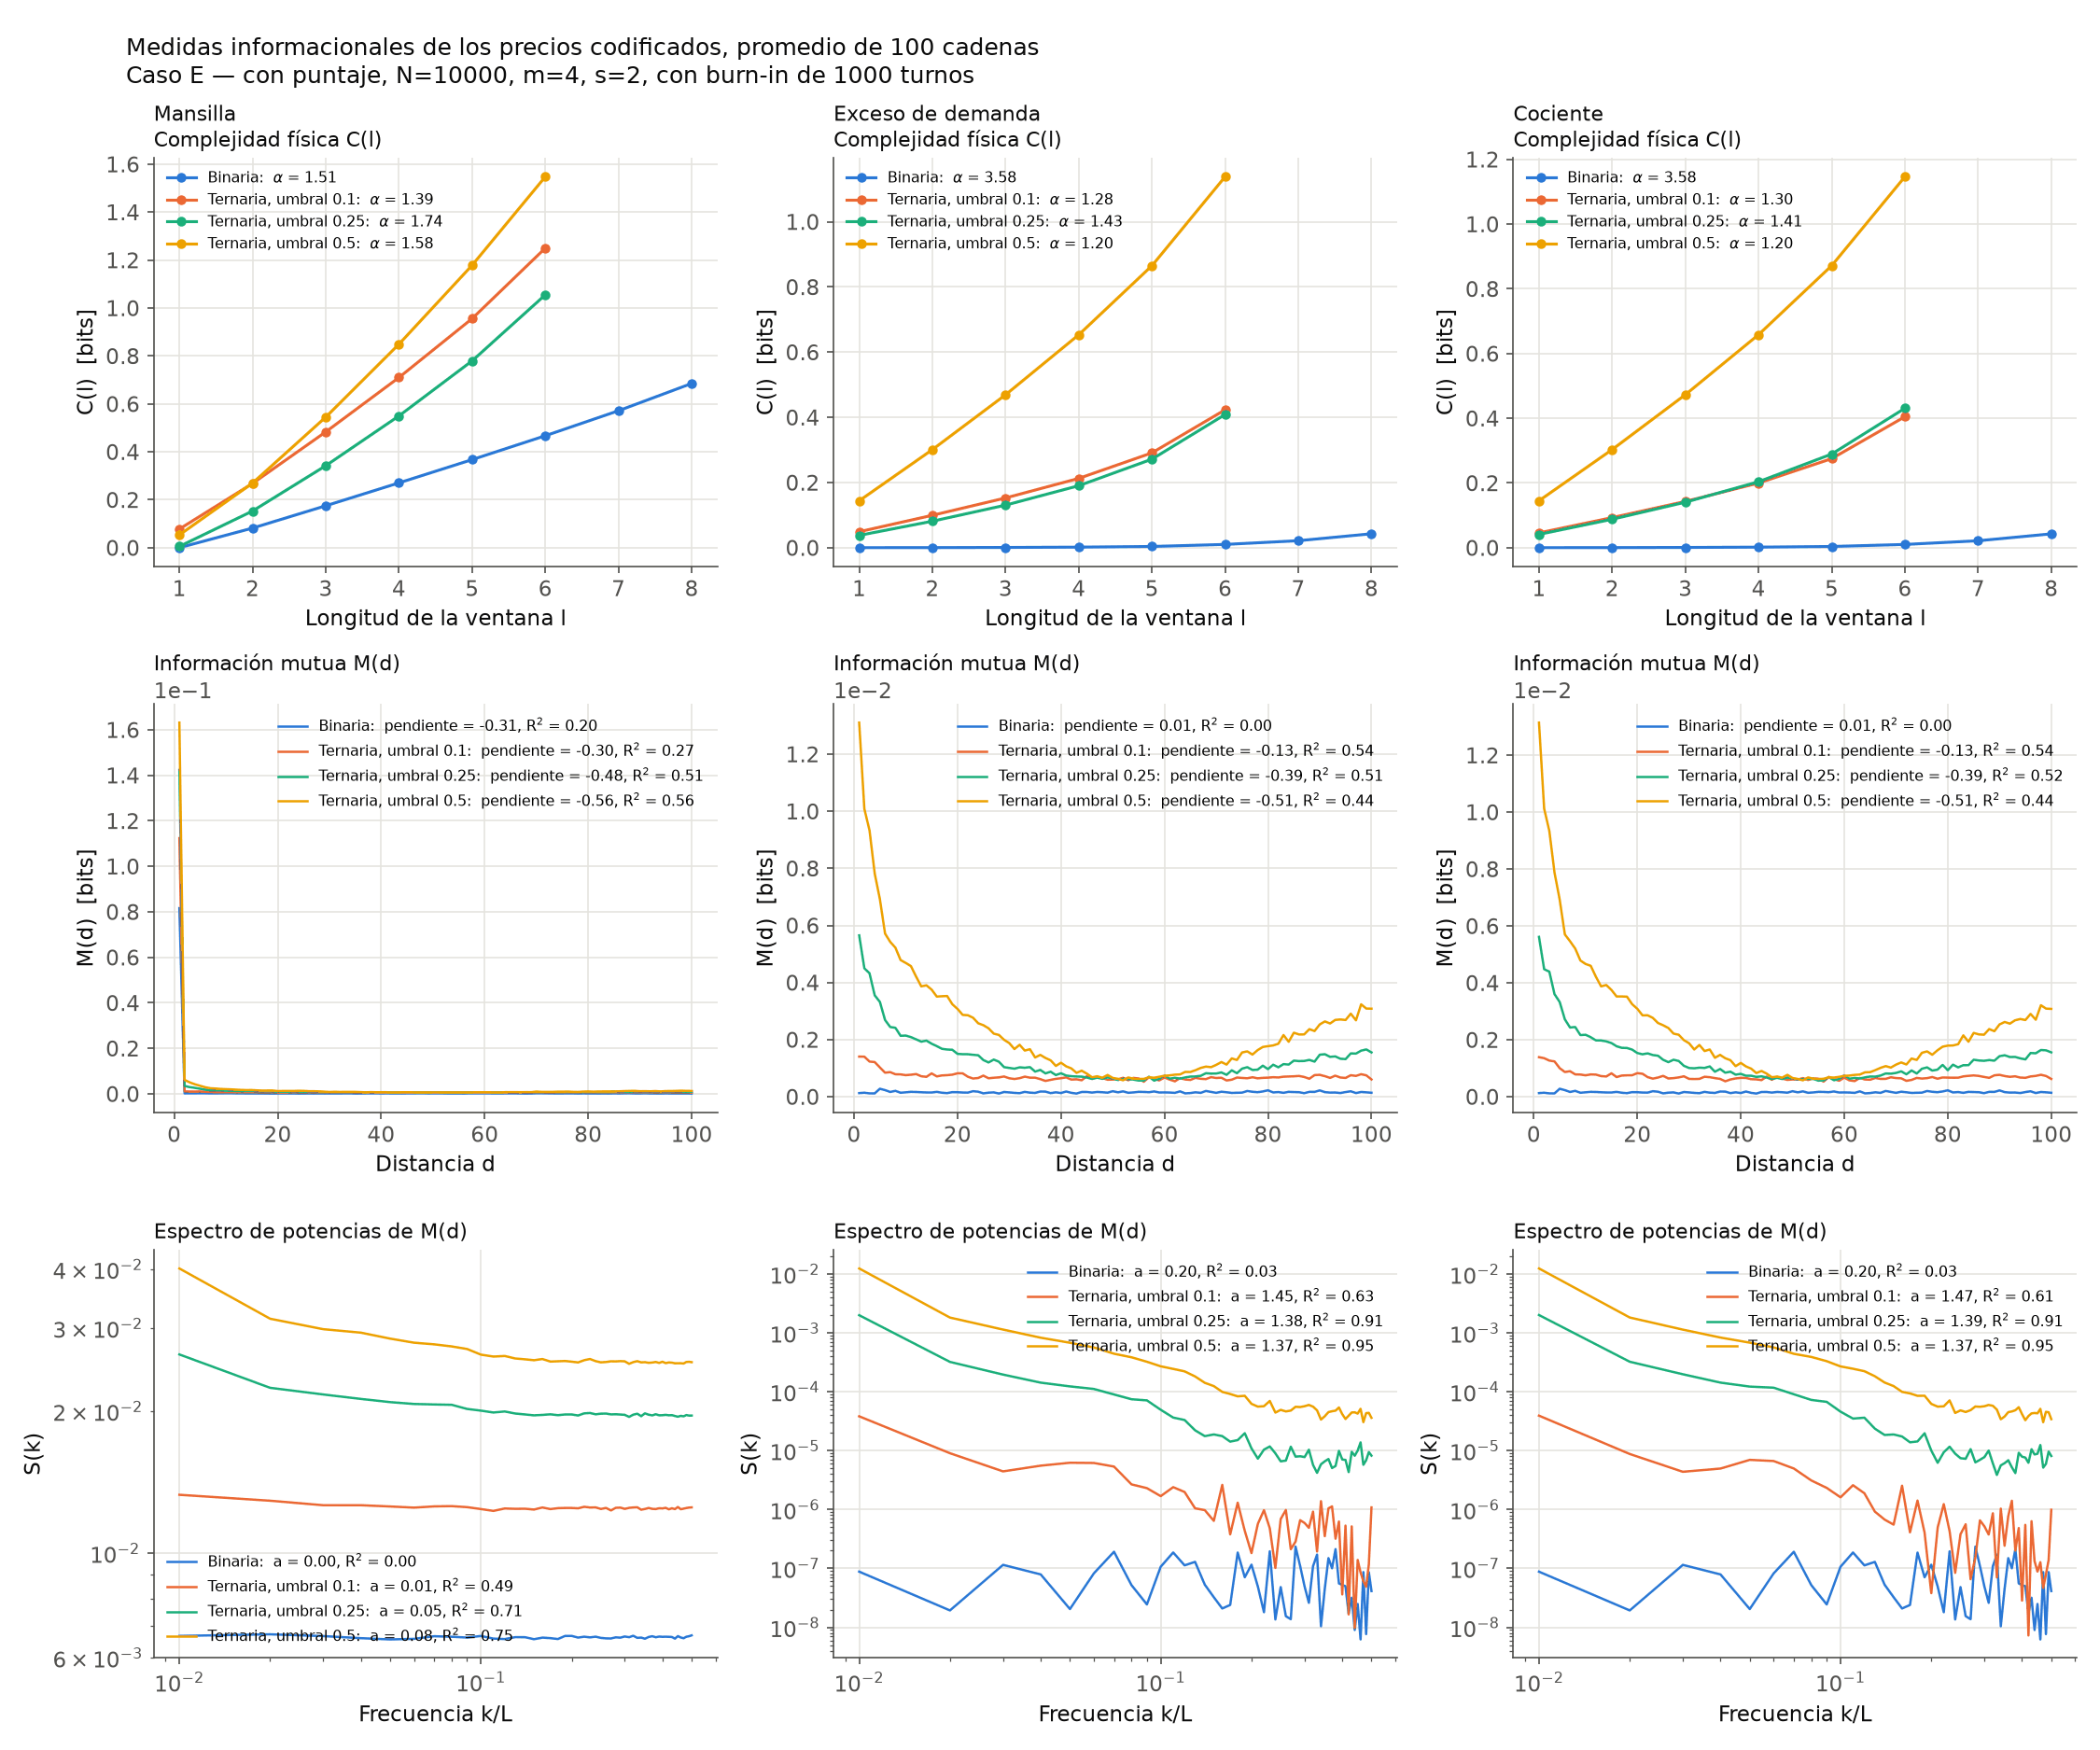
\includegraphics[width=0.85\textwidth]{figuras/Fase9_medidas_informacionales_casoE_N10000_m4_s2_con_puntaje_T6000_regla_nueva_con_burnin1000.png}
\caption{Caso E: medidas informacionales de los precios codificados, con burn-in.}
\end{figure}

\clearpage
\subsection{Caso F: $m=5$, con puntaje}
\begin{figure}[H]
\centering
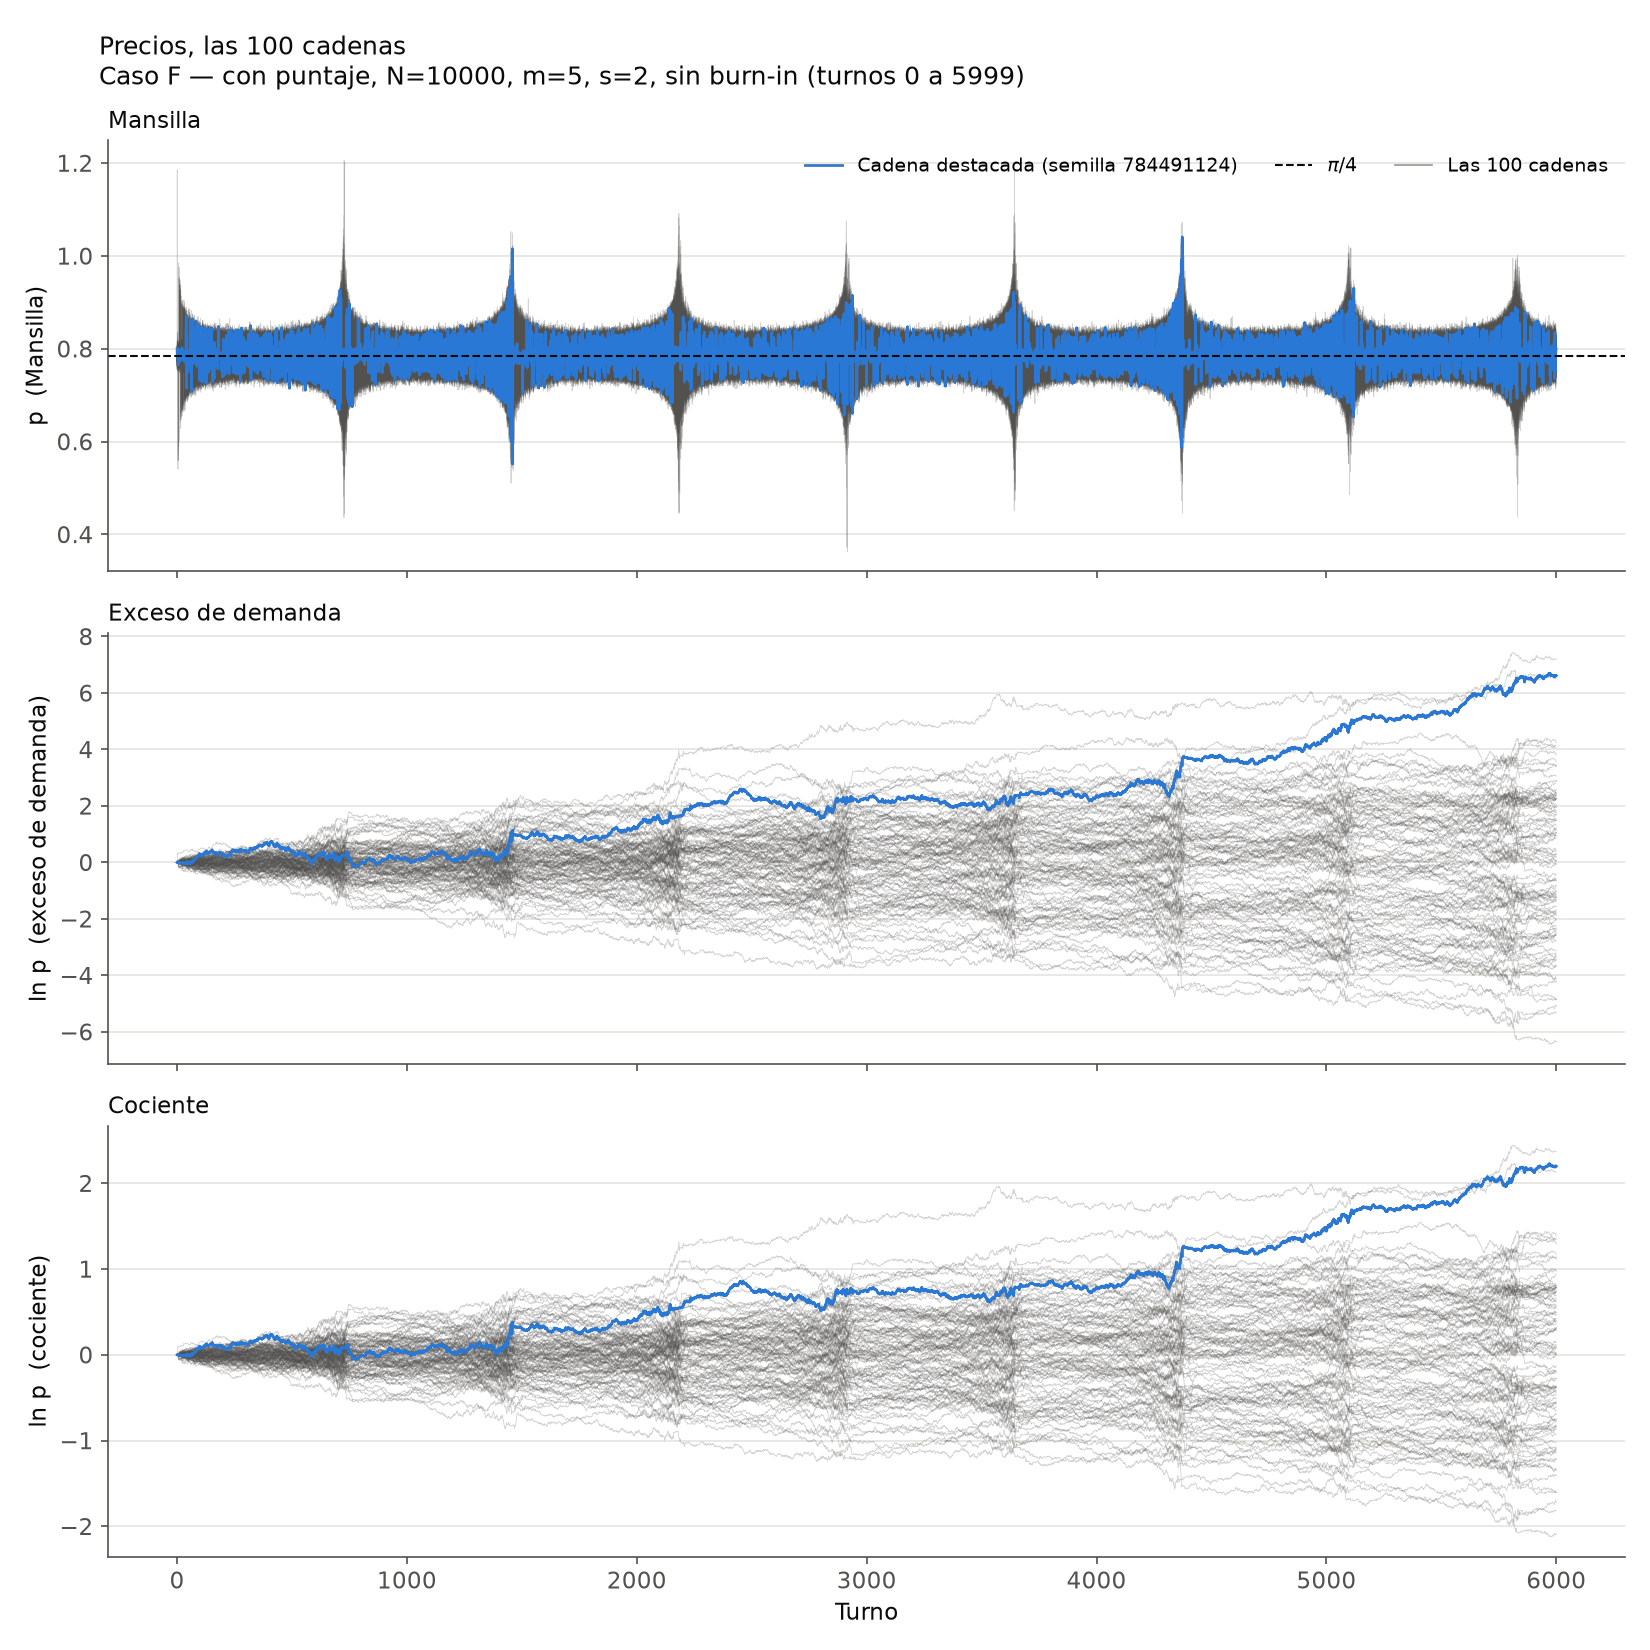
\includegraphics[width=0.49\textwidth]{figuras/Fase9_precios_conjunto_casoF_N10000_m5_s2_con_puntaje_T6000_regla_nueva_sin_burnin.png}\hfill
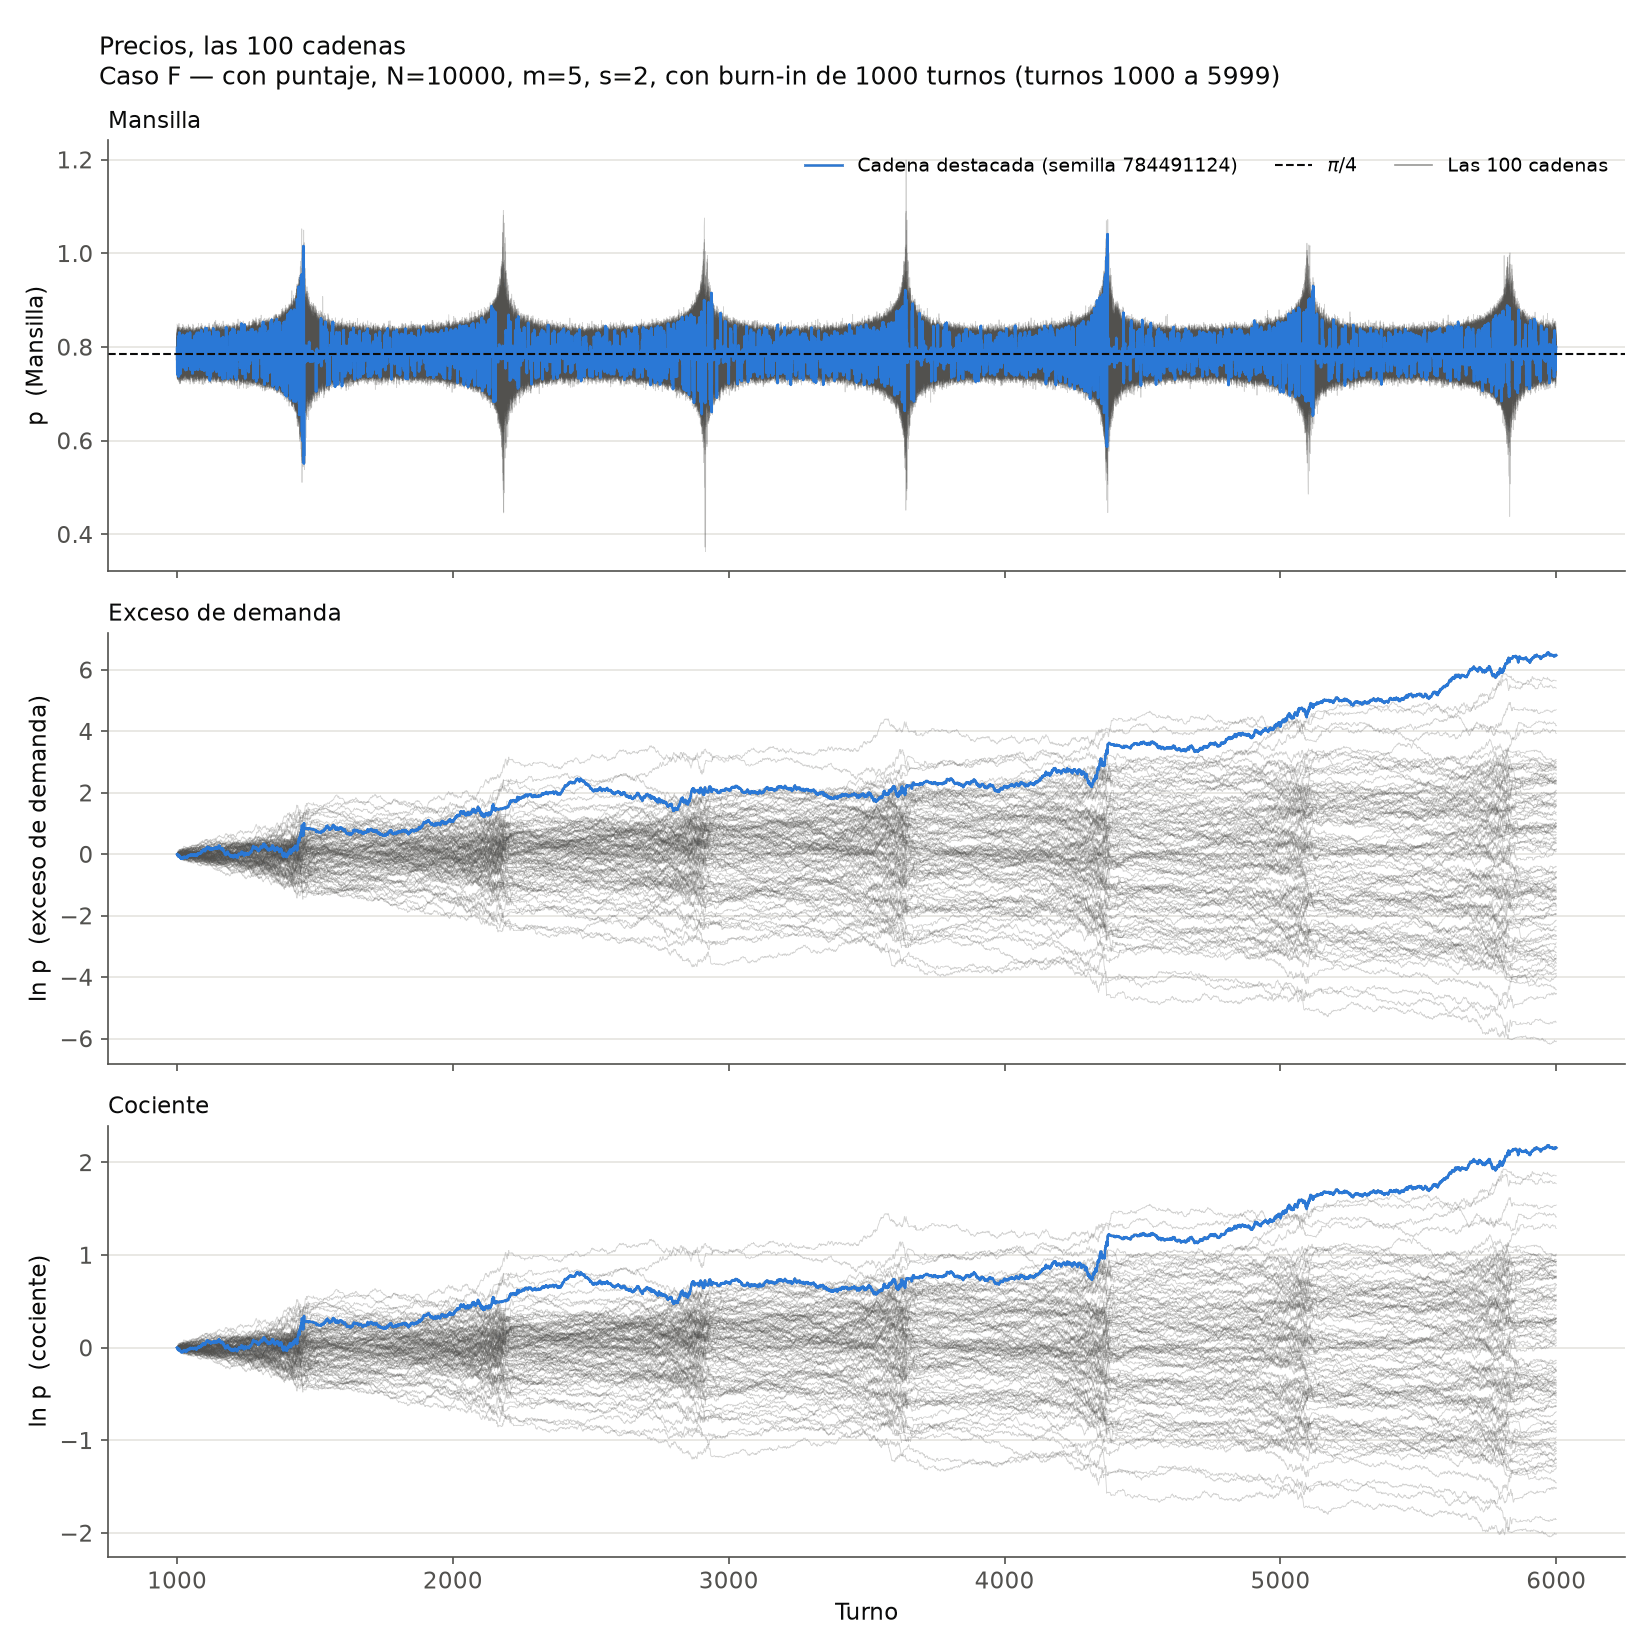
\includegraphics[width=0.49\textwidth]{figuras/Fase9_precios_conjunto_casoF_N10000_m5_s2_con_puntaje_T6000_regla_nueva_con_burnin1000.png}
\caption{Caso F, $N=10000$: conjunto de precios sin burn-in (izquierda) y con burn-in (derecha).}
\end{figure}

\begin{figure}[H]
\centering
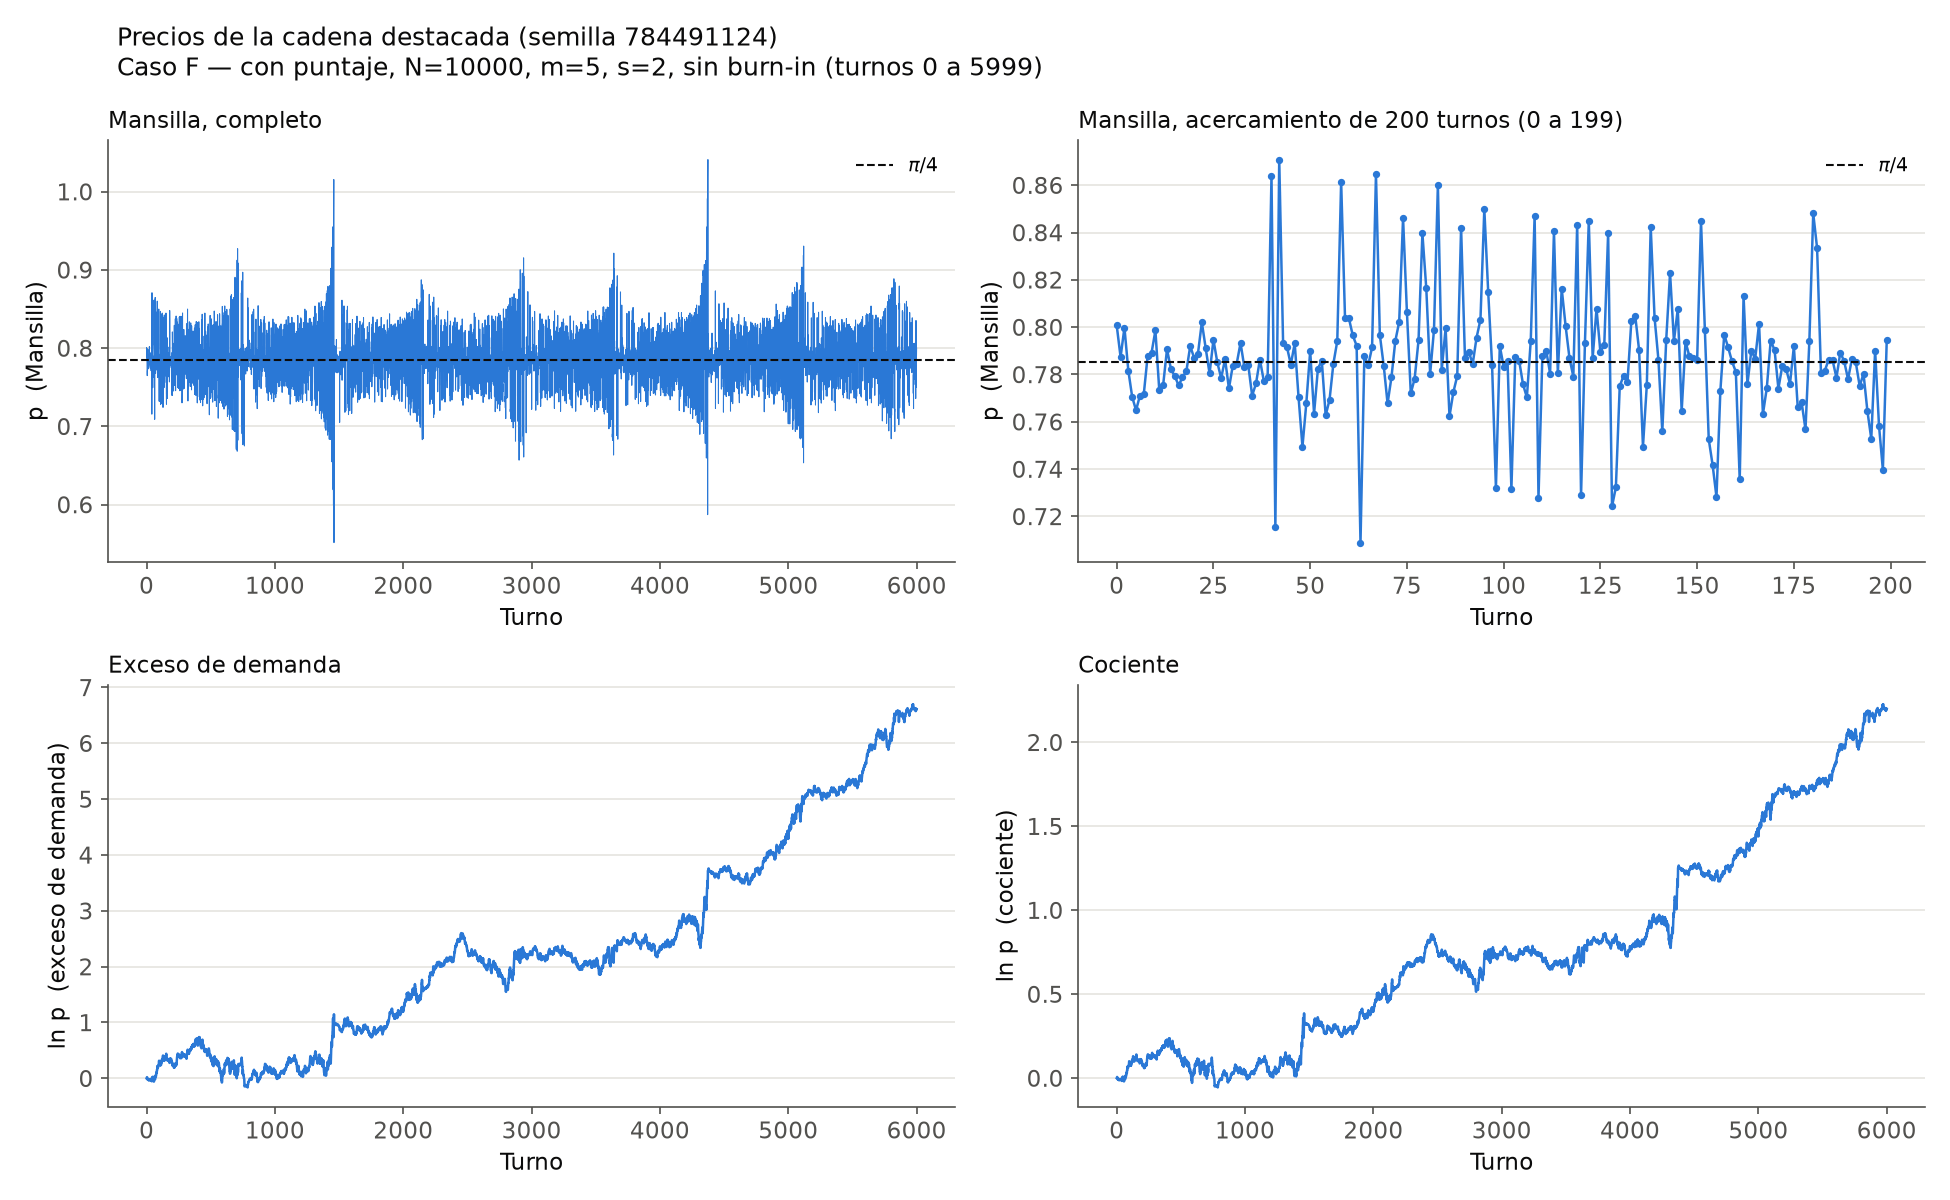
\includegraphics[width=0.49\textwidth]{figuras/Fase9_precios_detalle_casoF_N10000_m5_s2_con_puntaje_T6000_regla_nueva_sin_burnin.png}\hfill
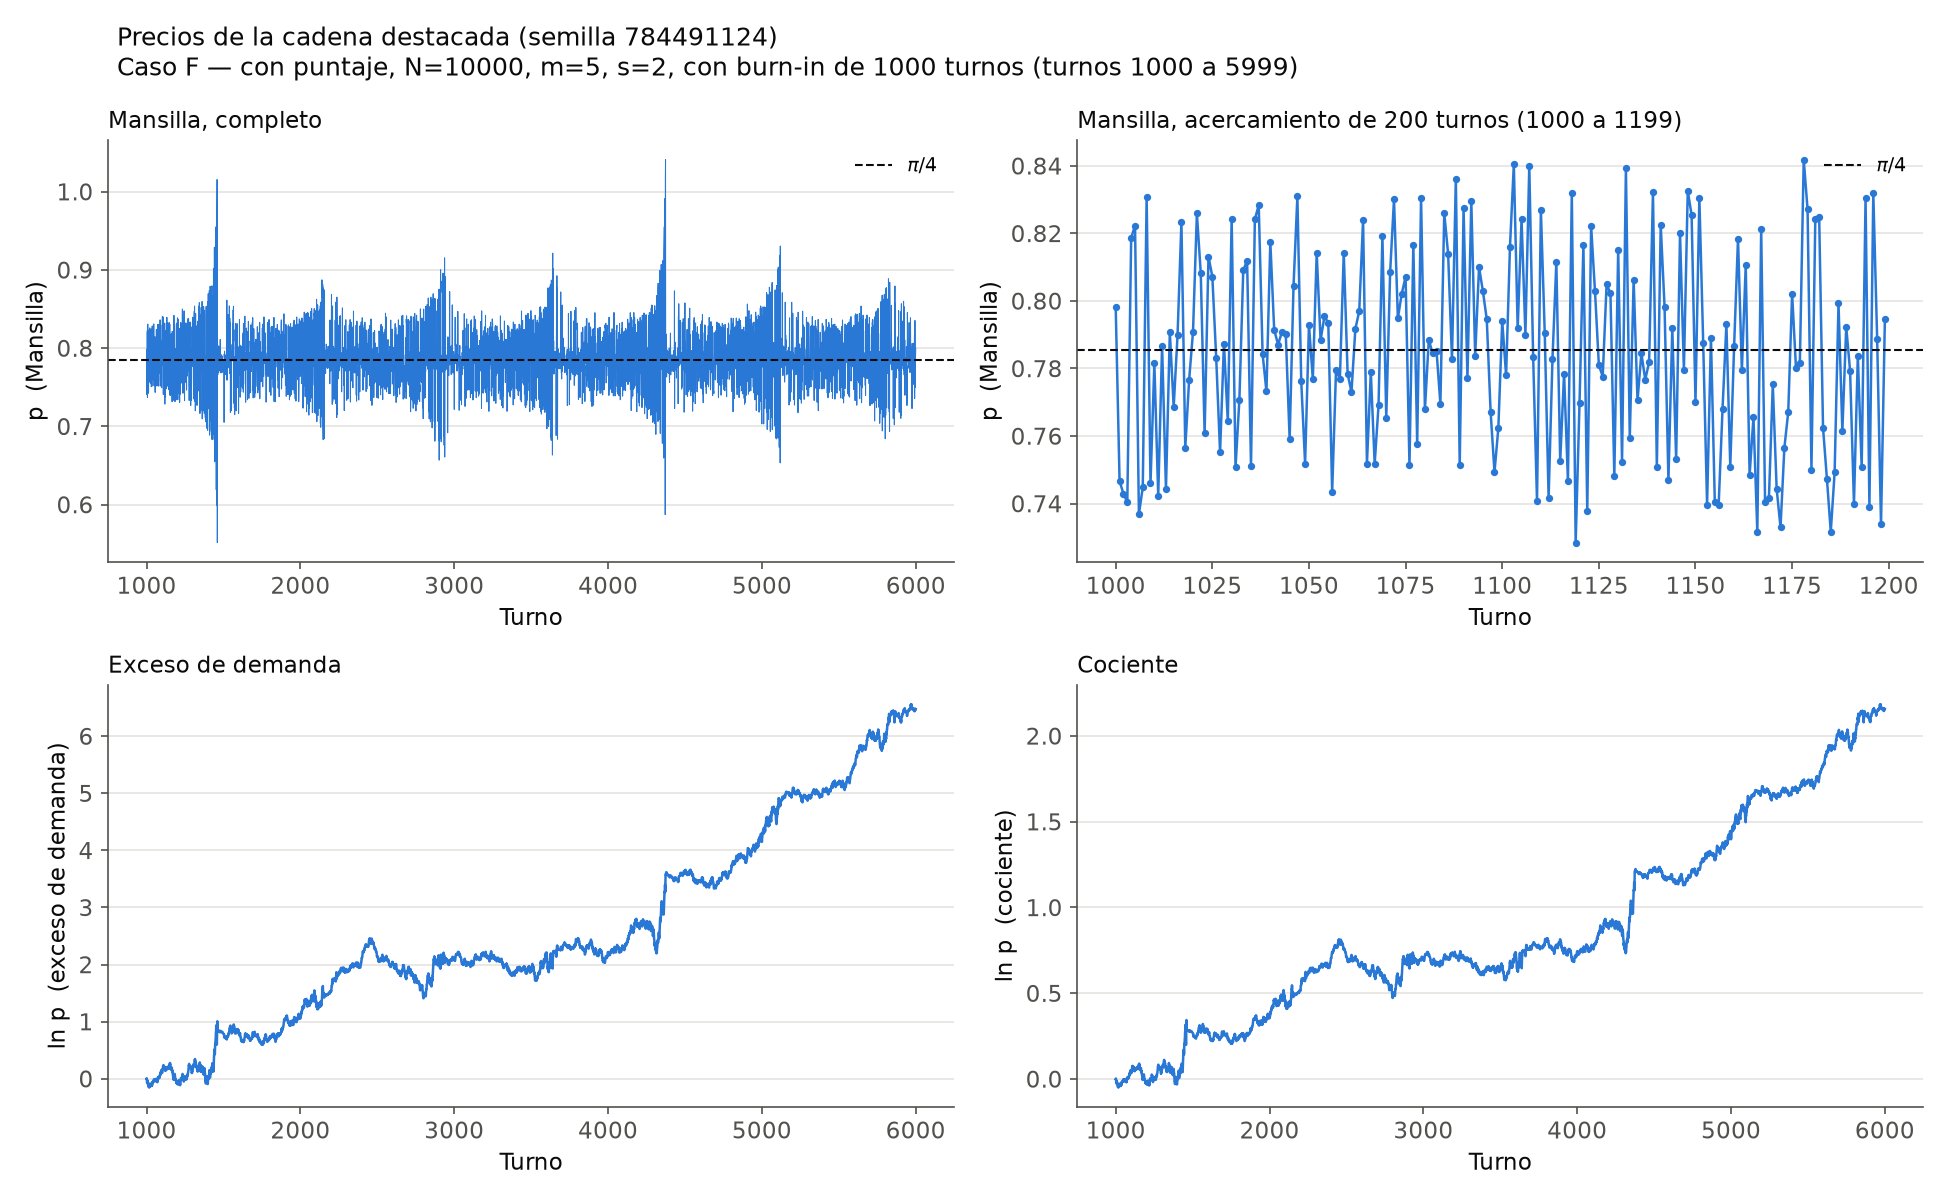
\includegraphics[width=0.49\textwidth]{figuras/Fase9_precios_detalle_casoF_N10000_m5_s2_con_puntaje_T6000_regla_nueva_con_burnin1000.png}
\caption{Caso F, $N=10000$: detalle de la cadena destacada sin burn-in (izquierda) y con burn-in (derecha).}
\end{figure}

\begin{figure}[H]
\centering
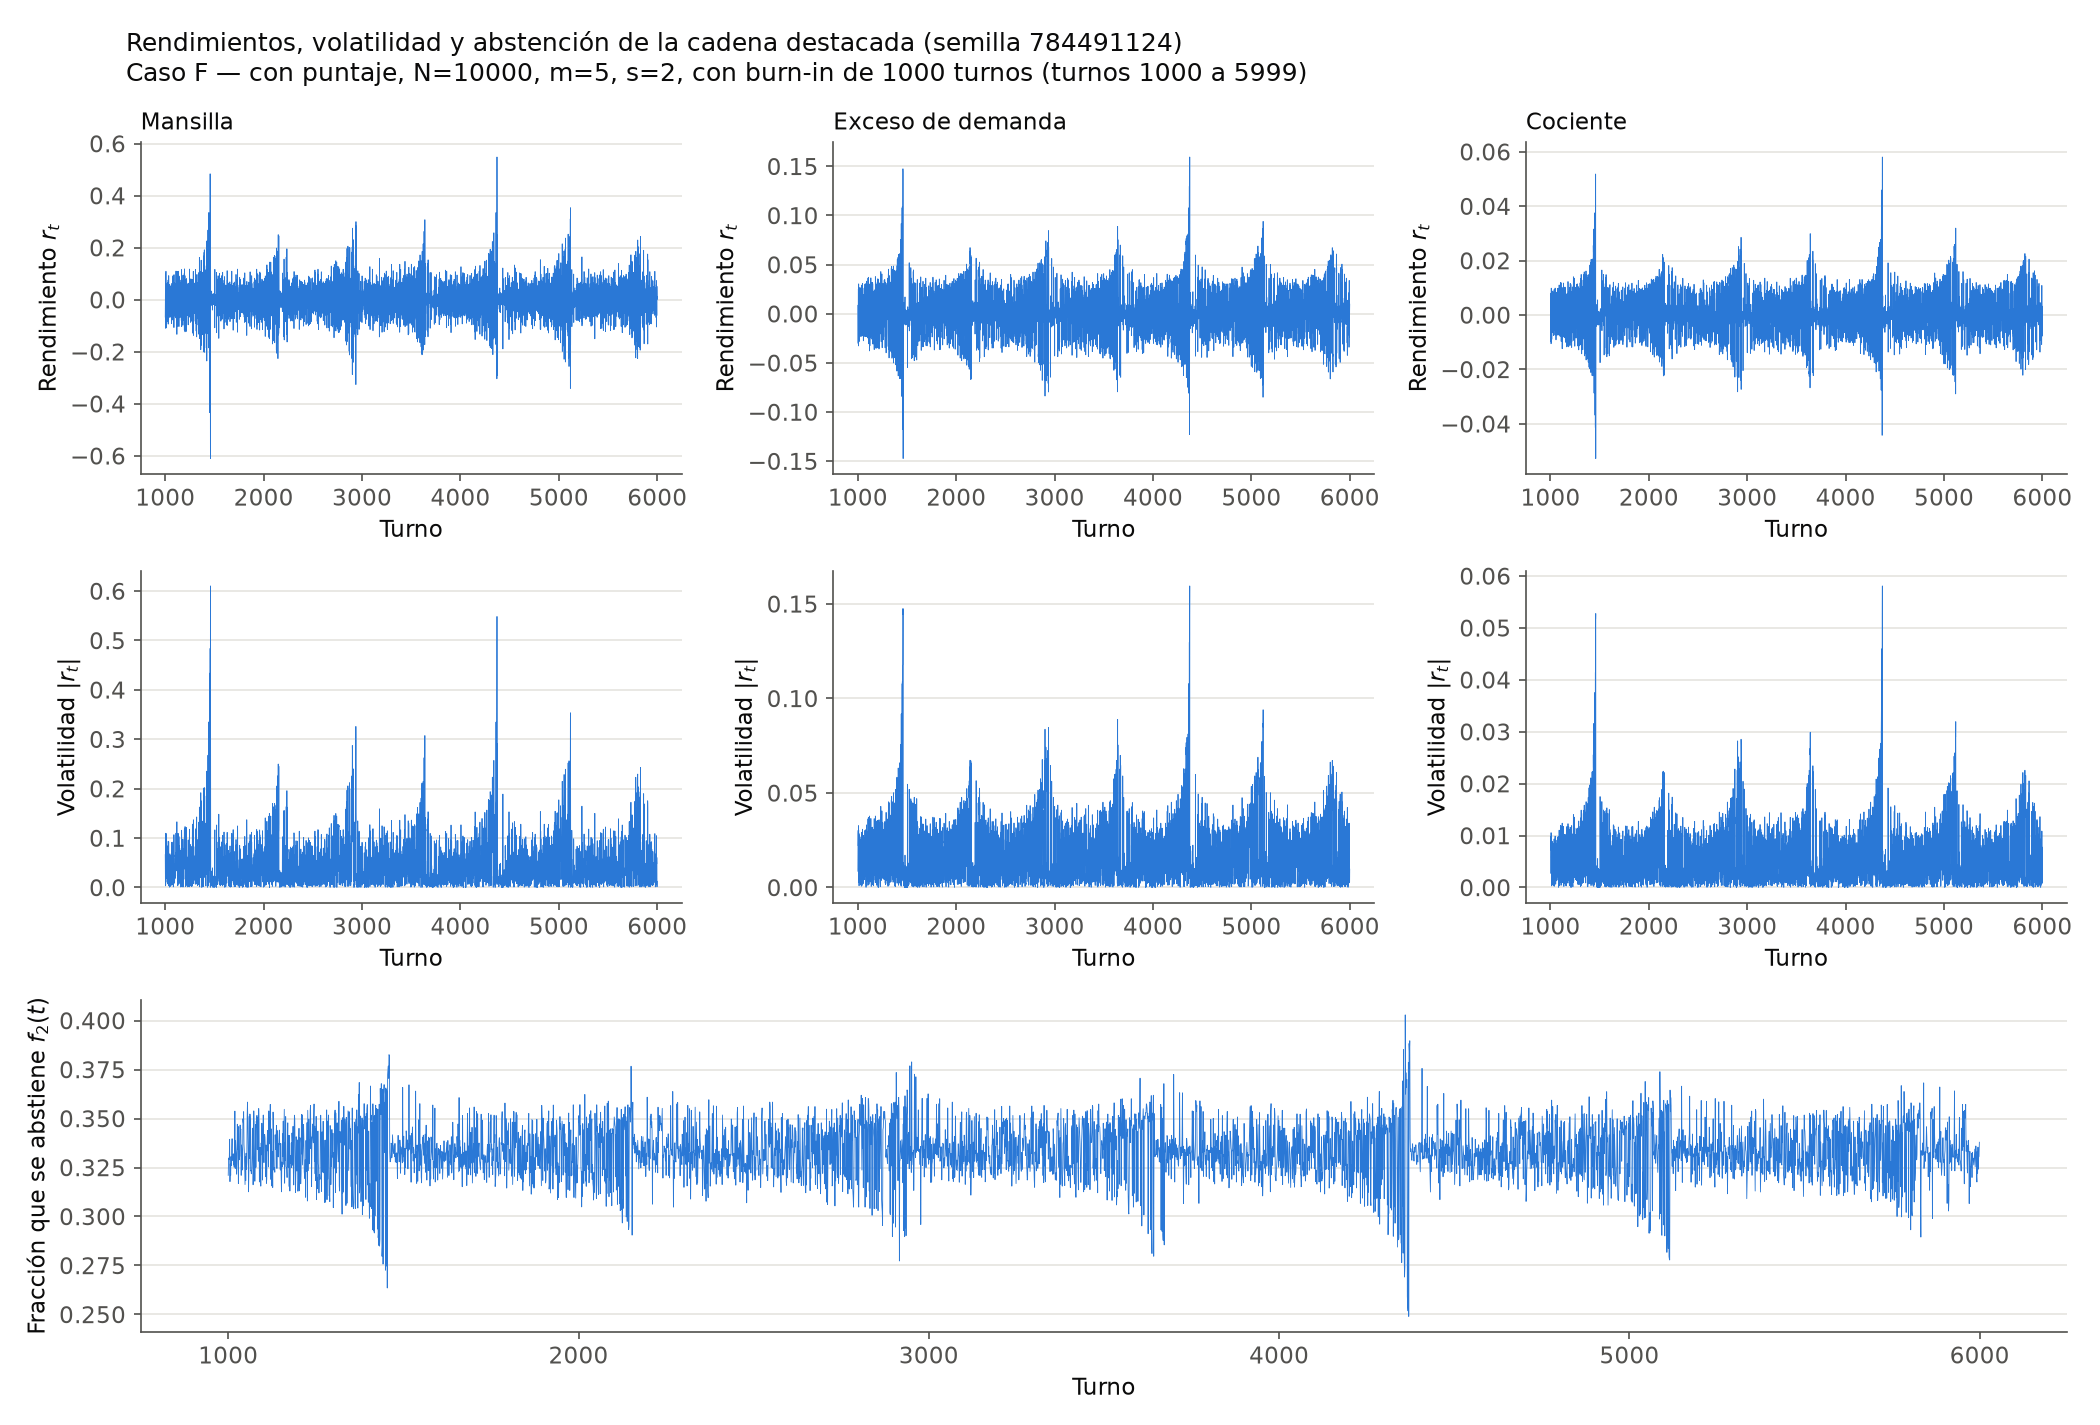
\includegraphics[width=0.85\textwidth]{figuras/Fase9_series_casoF_N10000_m5_s2_con_puntaje_T6000_regla_nueva_con_burnin1000.png}
\caption{Caso F: rendimientos, volatilidad y fracción que se abstiene de la cadena destacada, con burn-in.}
\end{figure}

\begin{figure}[H]
\centering
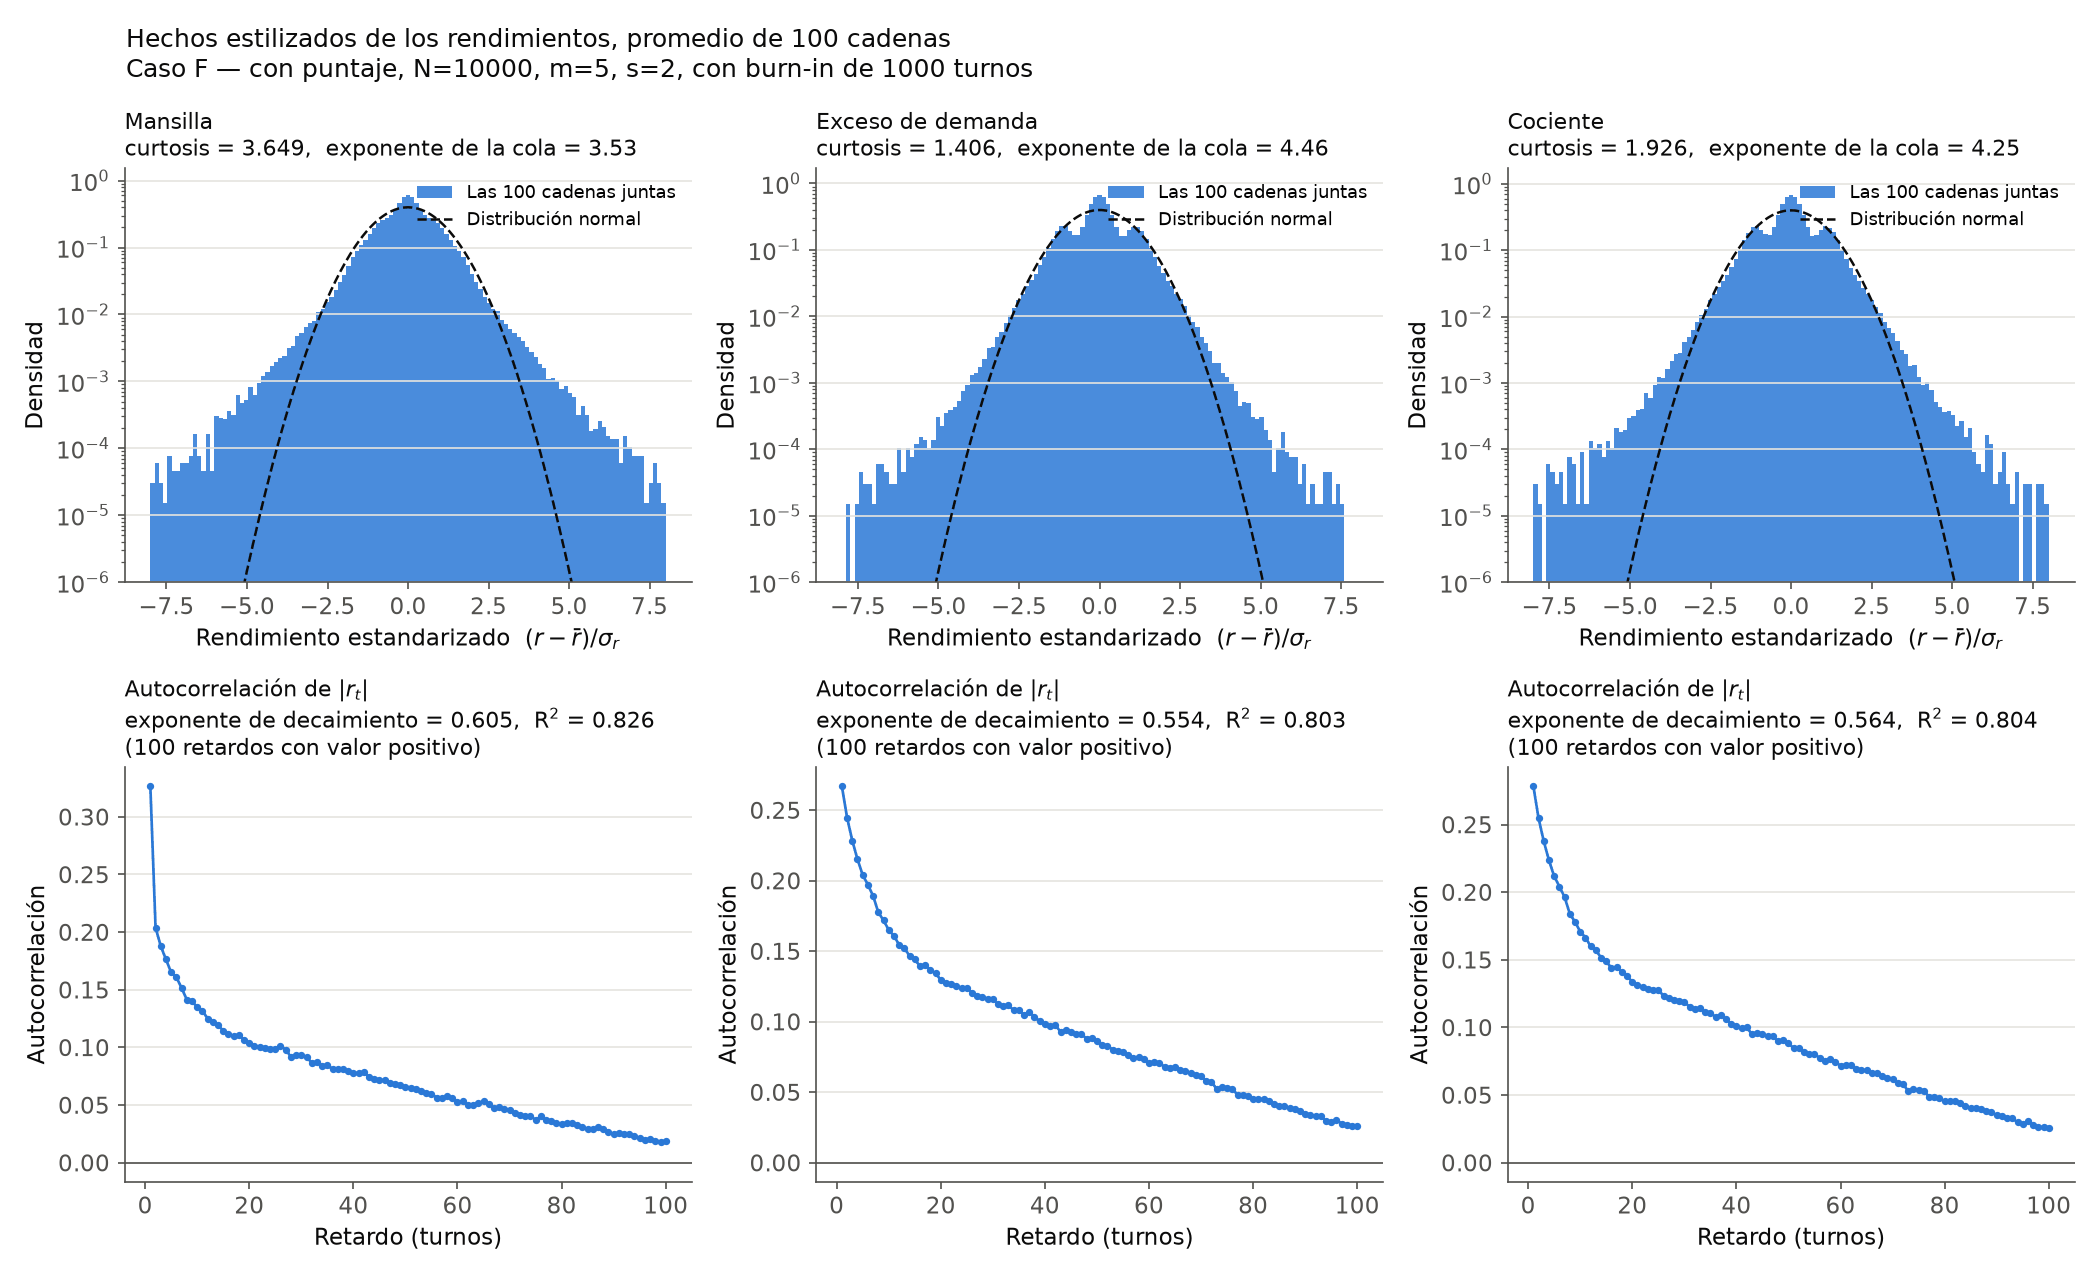
\includegraphics[width=0.85\textwidth]{figuras/Fase9_hechos_estilizados_casoF_N10000_m5_s2_con_puntaje_T6000_regla_nueva_con_burnin1000.png}
\caption{Caso F: hechos estilizados (distribución de los rendimientos y autocorrelación de $|r|$), con burn-in.}
\end{figure}

\begin{figure}[H]
\centering
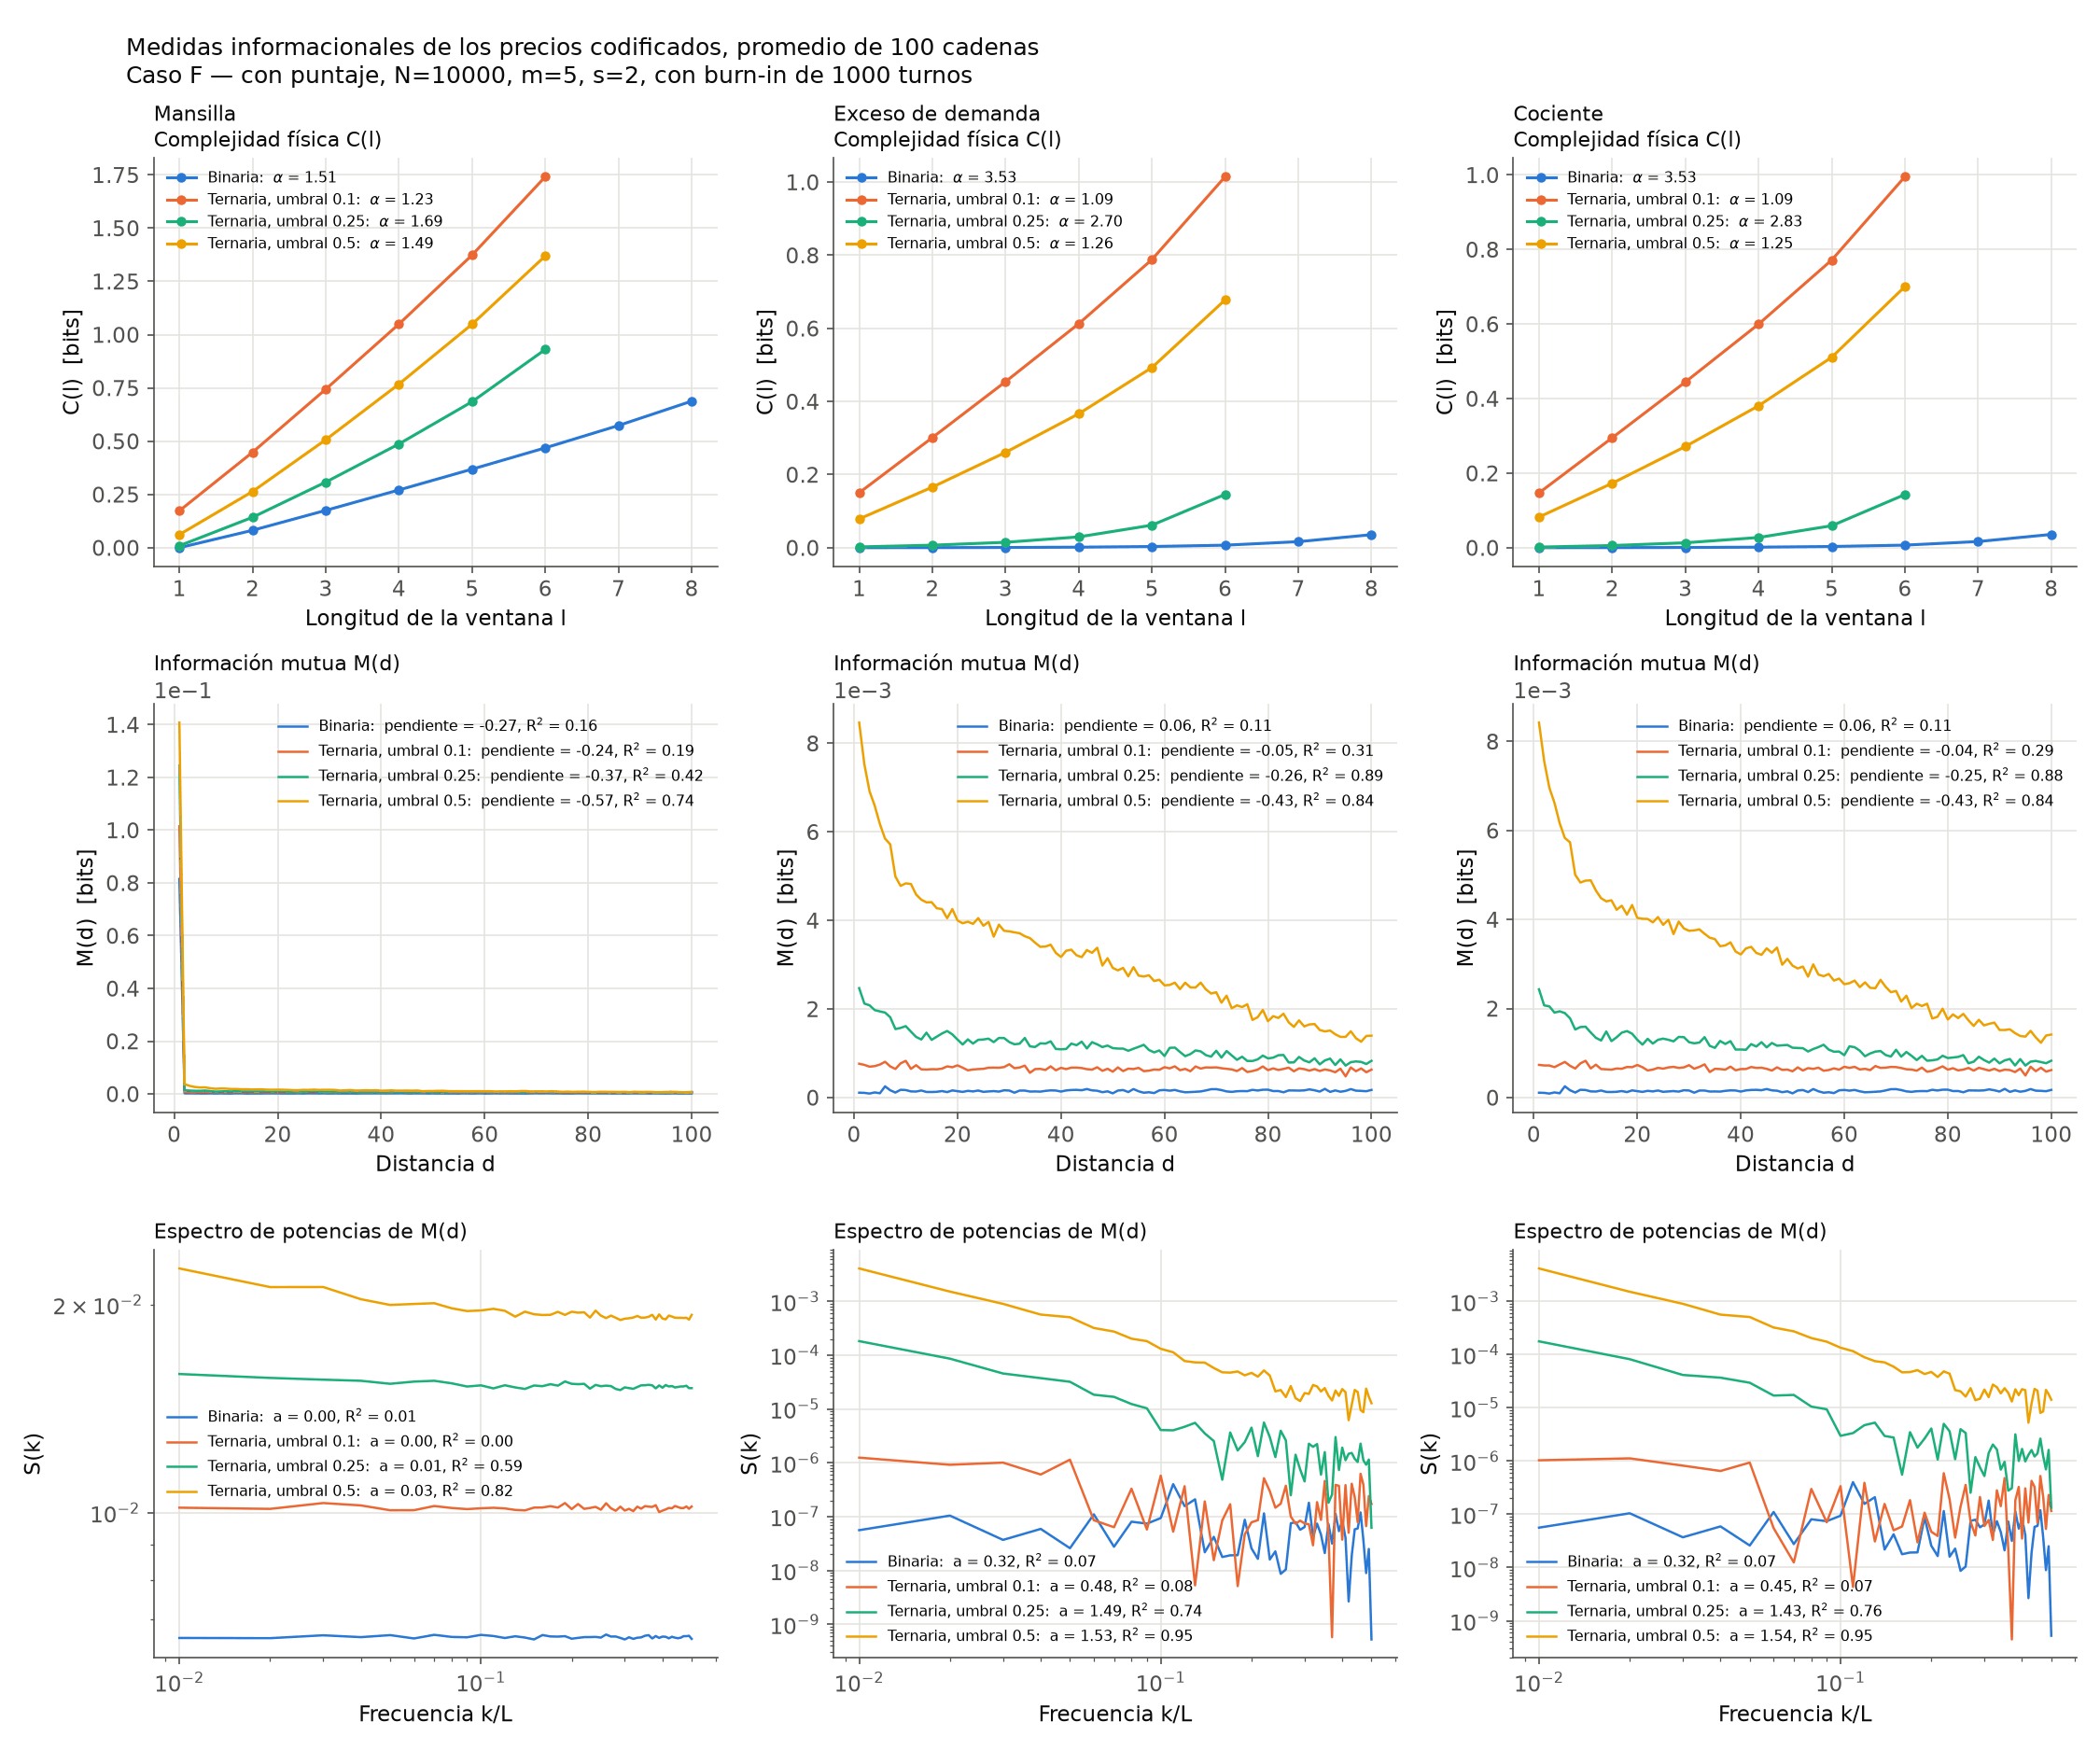
\includegraphics[width=0.85\textwidth]{figuras/Fase9_medidas_informacionales_casoF_N10000_m5_s2_con_puntaje_T6000_regla_nueva_con_burnin1000.png}
\caption{Caso F: medidas informacionales de los precios codificados, con burn-in.}
\end{figure}

\clearpage
\subsection{Caso G: $m=6$, con puntaje}
\begin{figure}[H]
\centering
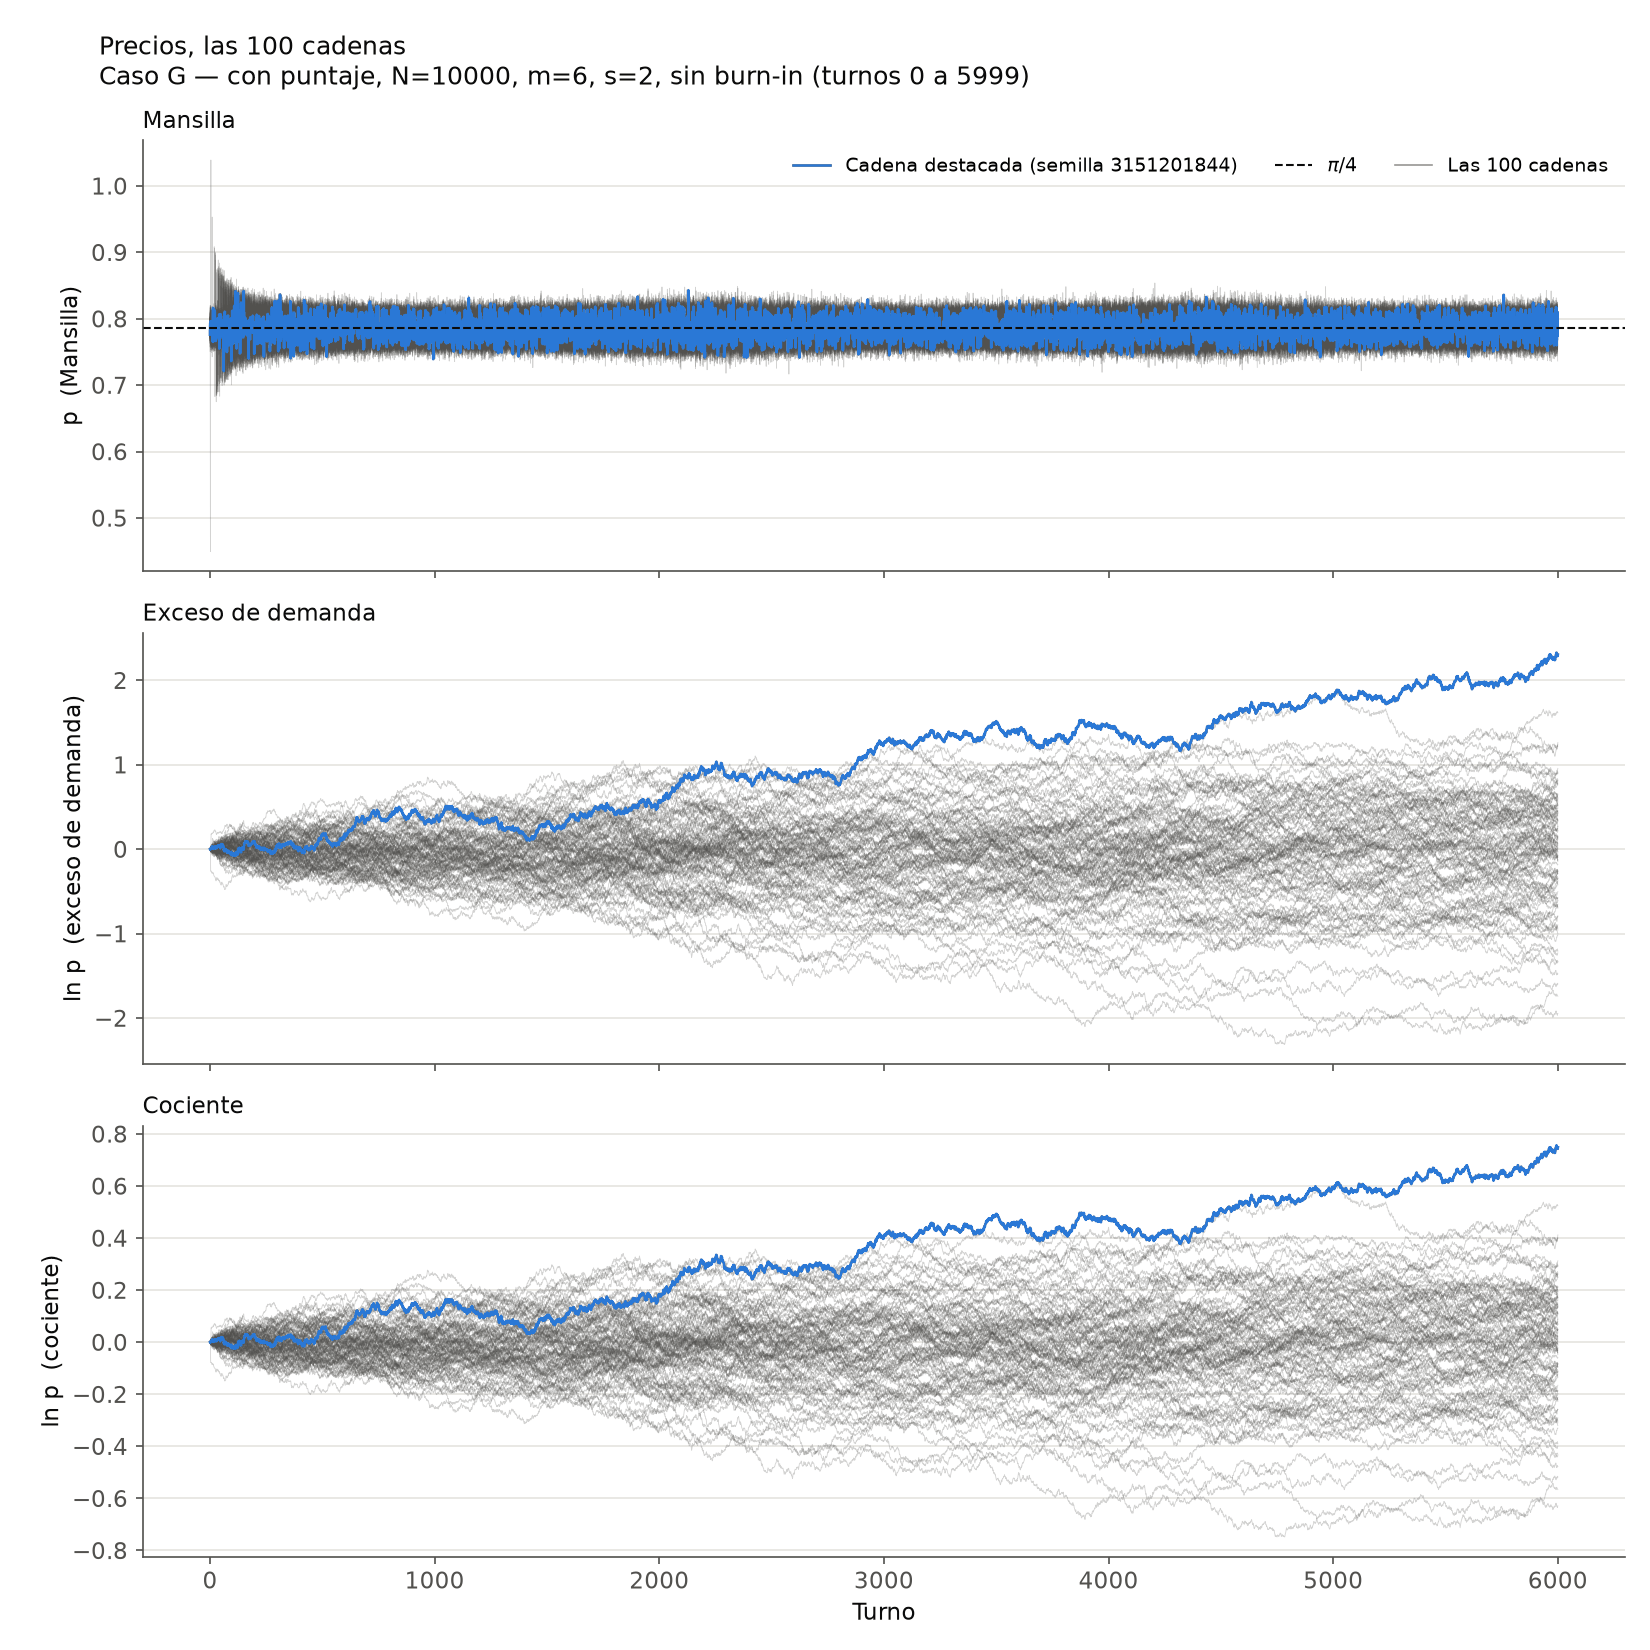
\includegraphics[width=0.49\textwidth]{figuras/Fase9_precios_conjunto_casoG_N10000_m6_s2_con_puntaje_T6000_regla_nueva_sin_burnin.png}\hfill
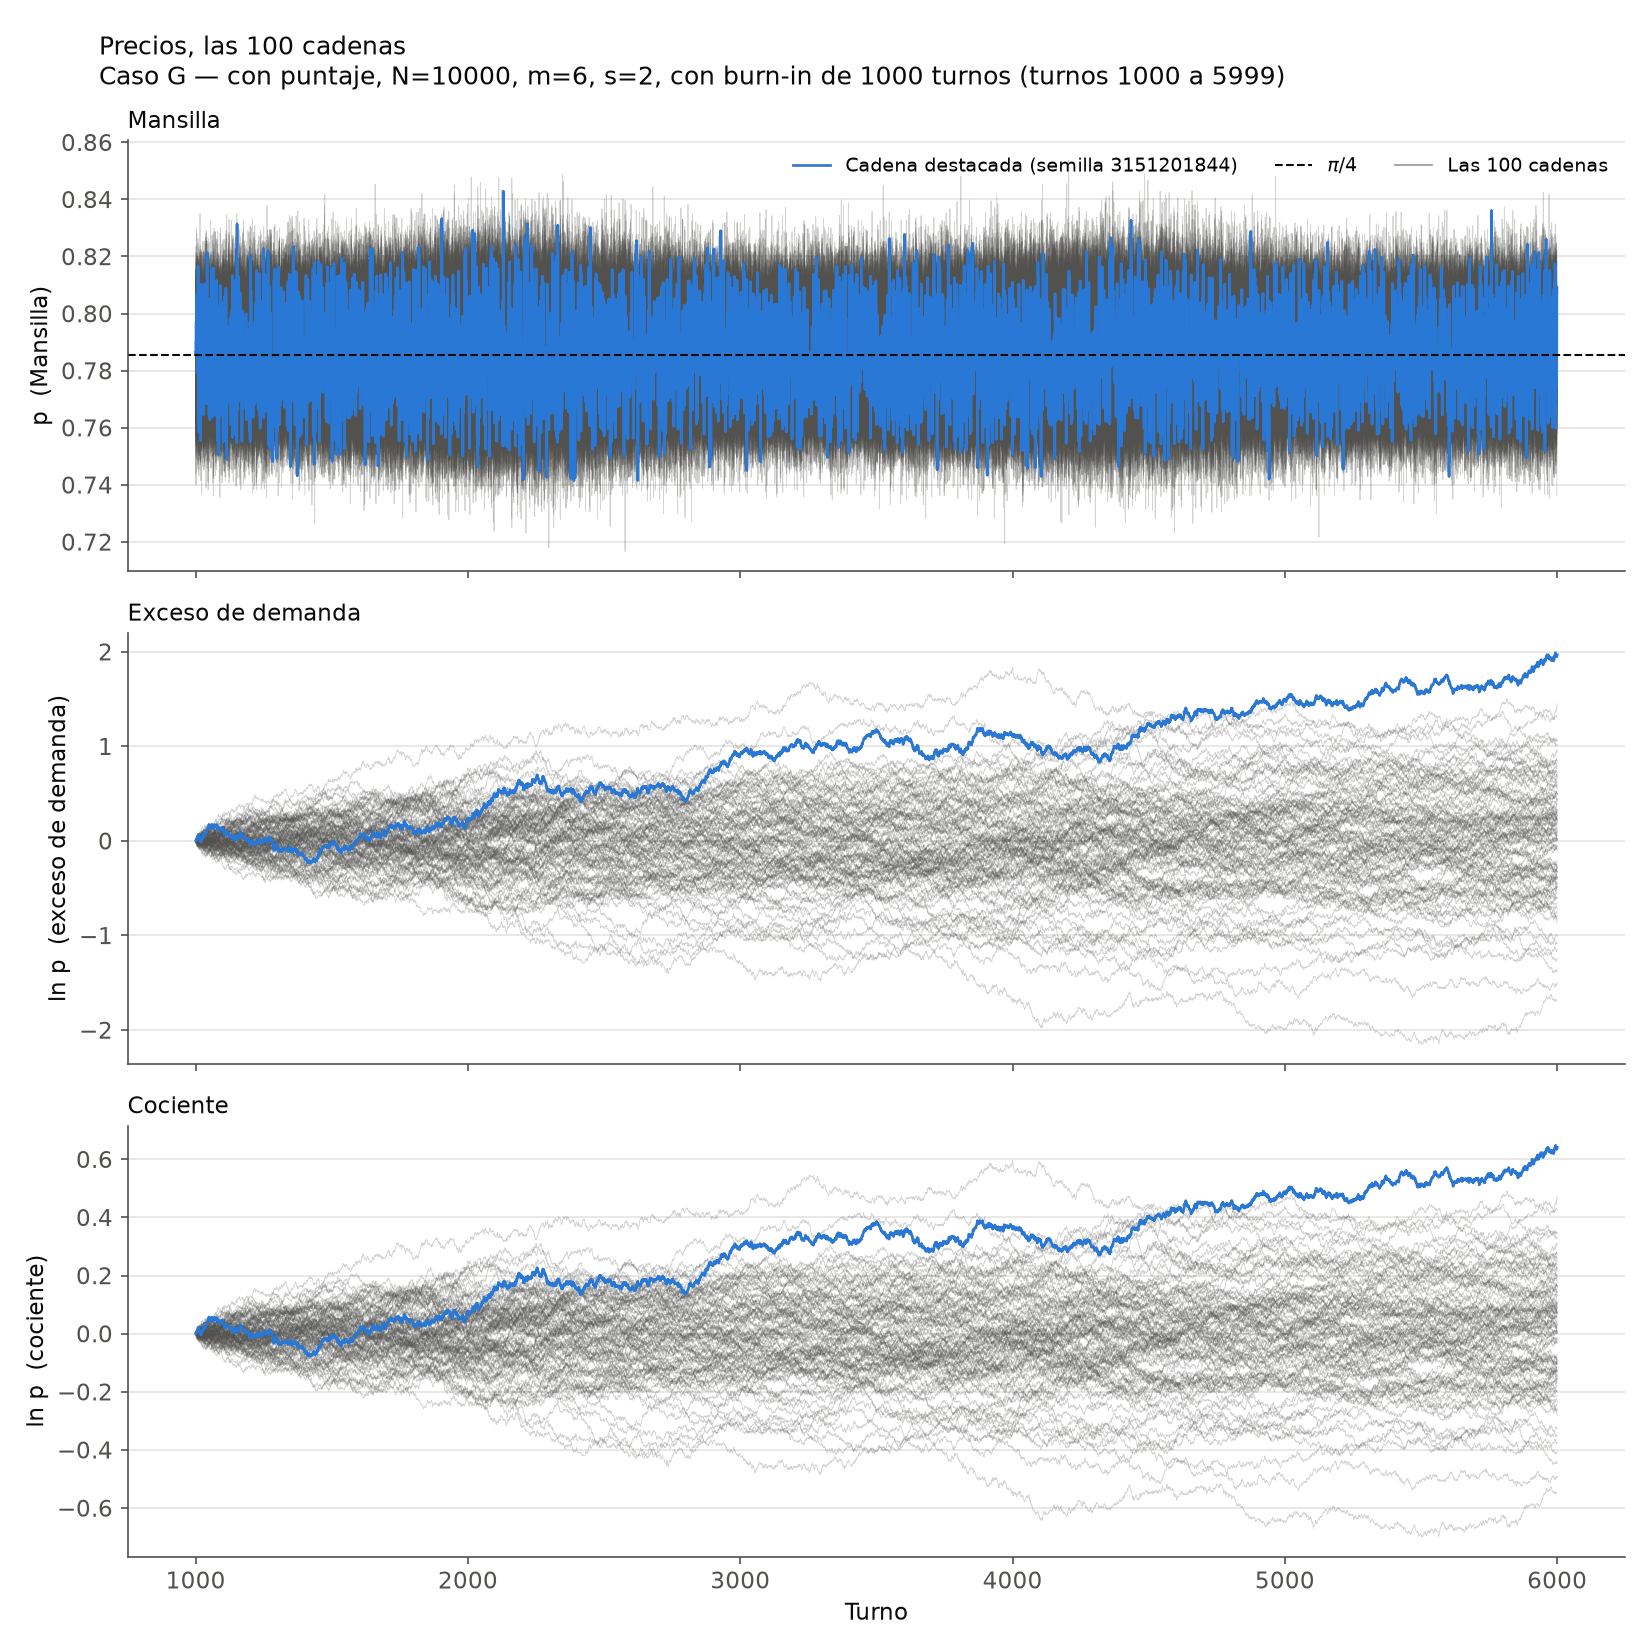
\includegraphics[width=0.49\textwidth]{figuras/Fase9_precios_conjunto_casoG_N10000_m6_s2_con_puntaje_T6000_regla_nueva_con_burnin1000.png}
\caption{Caso G, $N=10000$: conjunto de precios sin burn-in (izquierda) y con burn-in (derecha).}
\end{figure}

\begin{figure}[H]
\centering
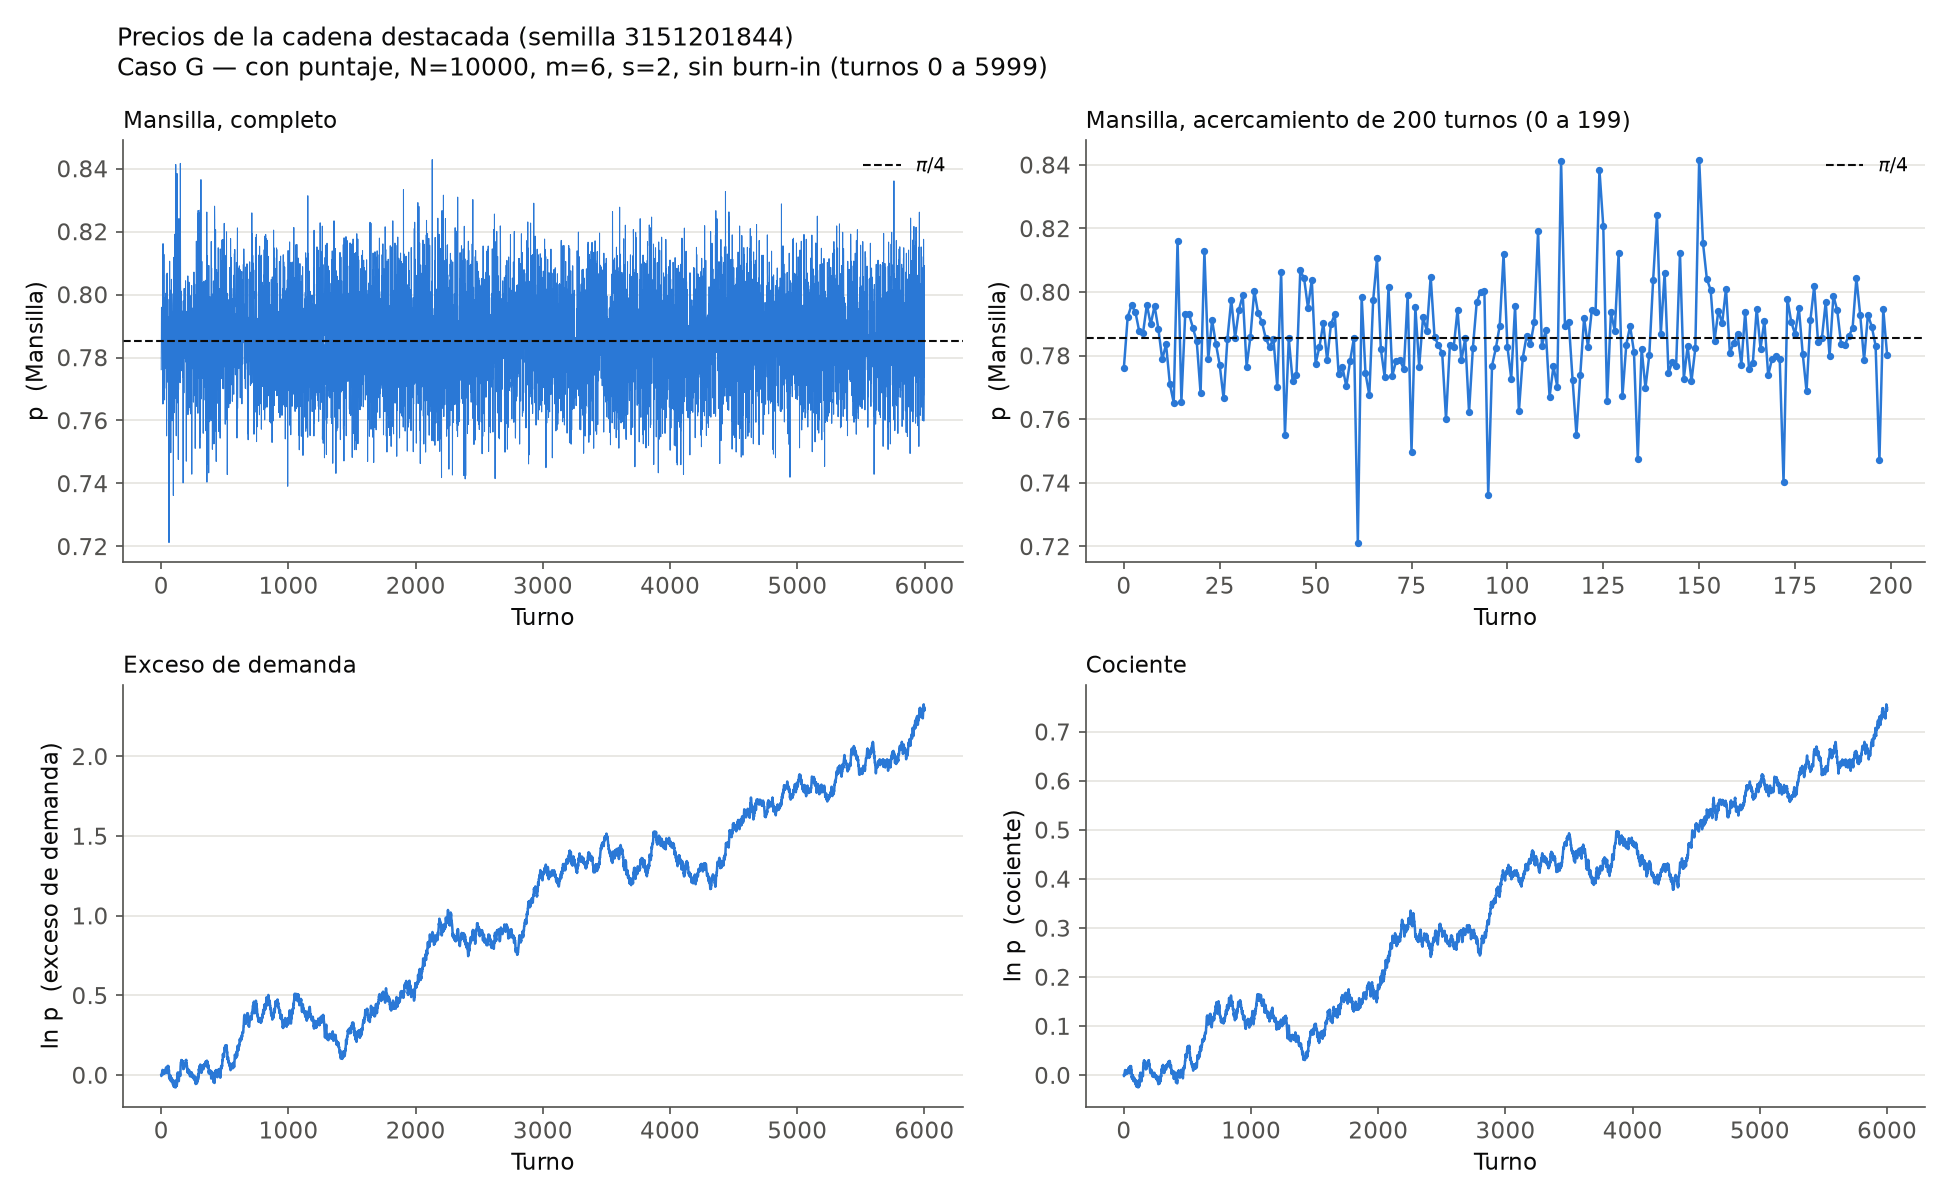
\includegraphics[width=0.49\textwidth]{figuras/Fase9_precios_detalle_casoG_N10000_m6_s2_con_puntaje_T6000_regla_nueva_sin_burnin.png}\hfill
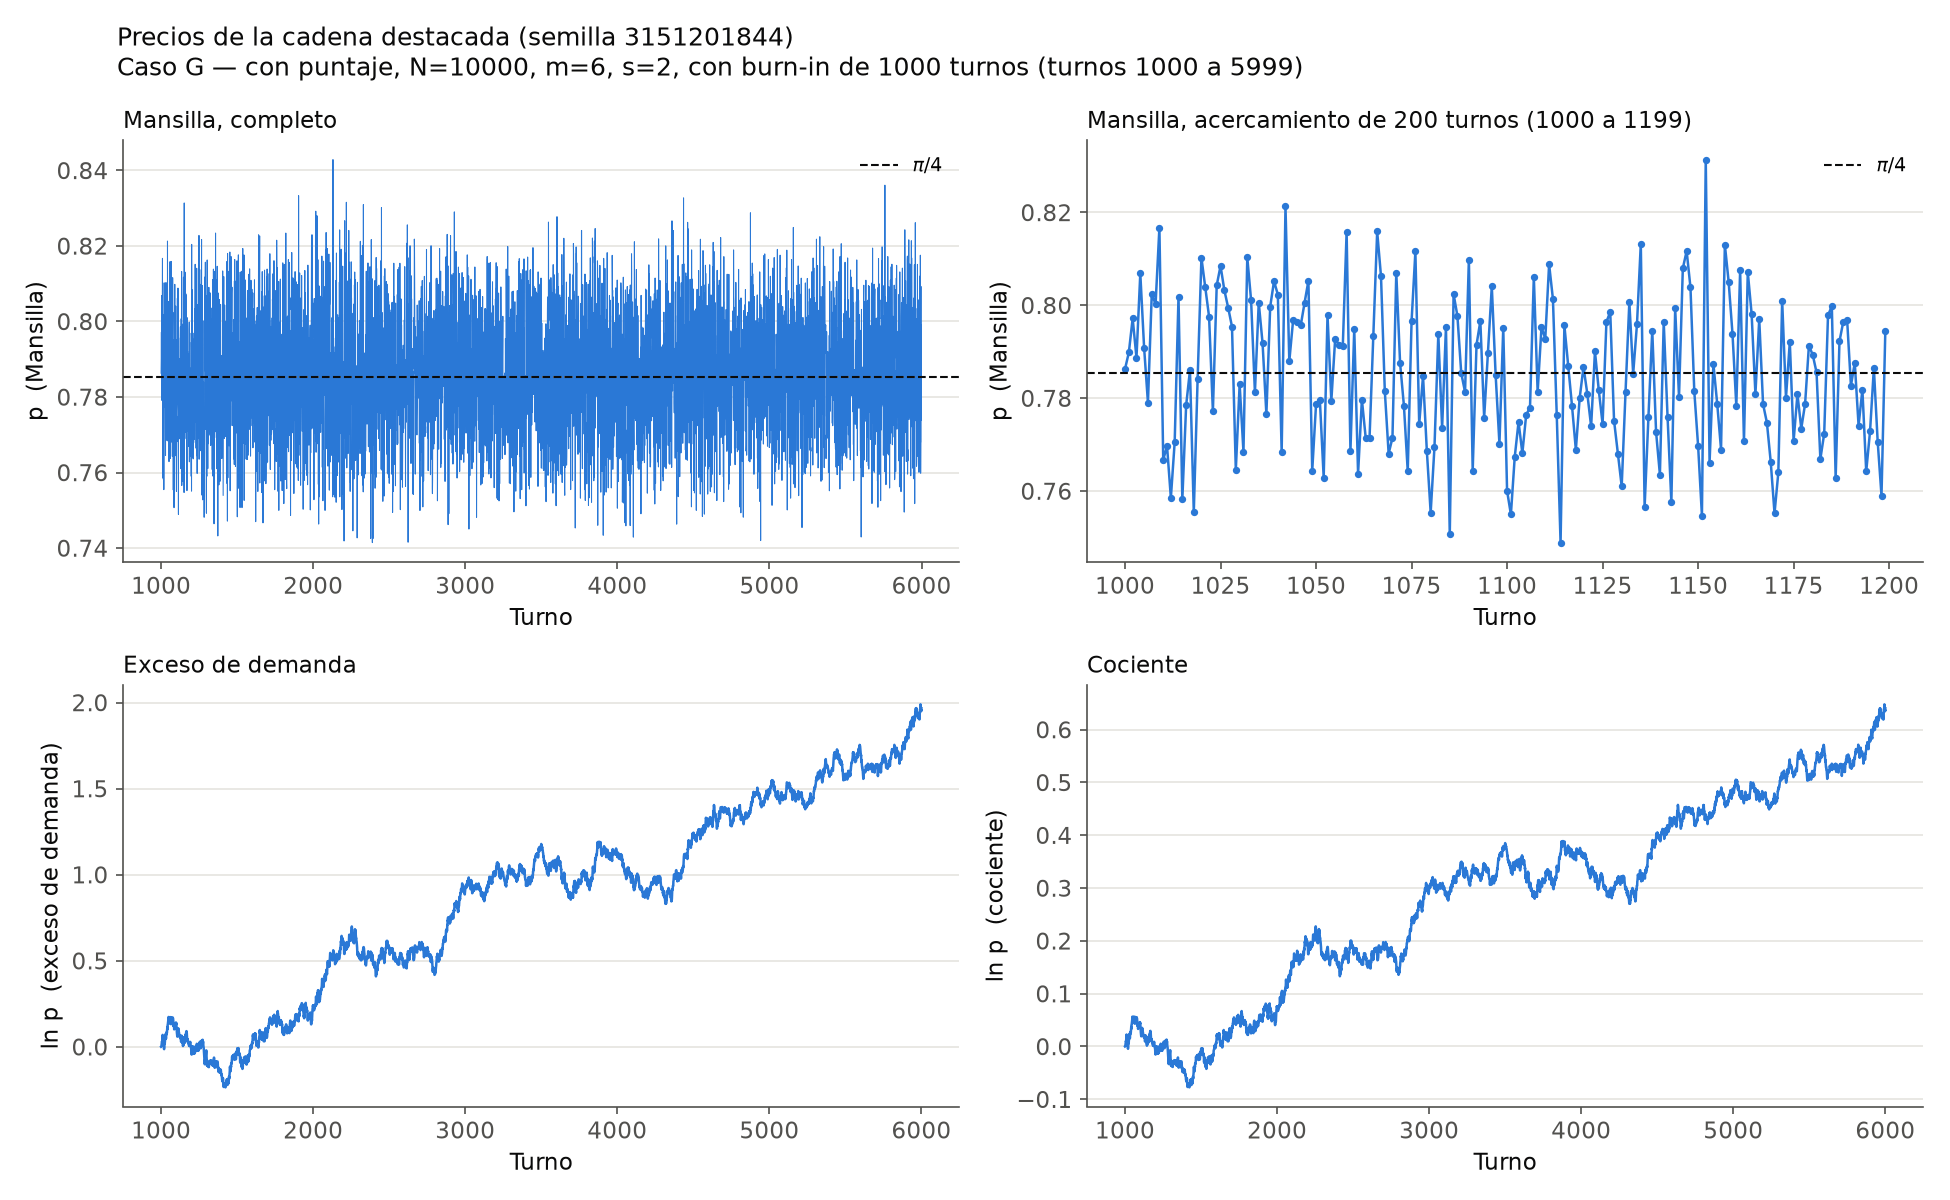
\includegraphics[width=0.49\textwidth]{figuras/Fase9_precios_detalle_casoG_N10000_m6_s2_con_puntaje_T6000_regla_nueva_con_burnin1000.png}
\caption{Caso G, $N=10000$: detalle de la cadena destacada sin burn-in (izquierda) y con burn-in (derecha).}
\end{figure}

\begin{figure}[H]
\centering
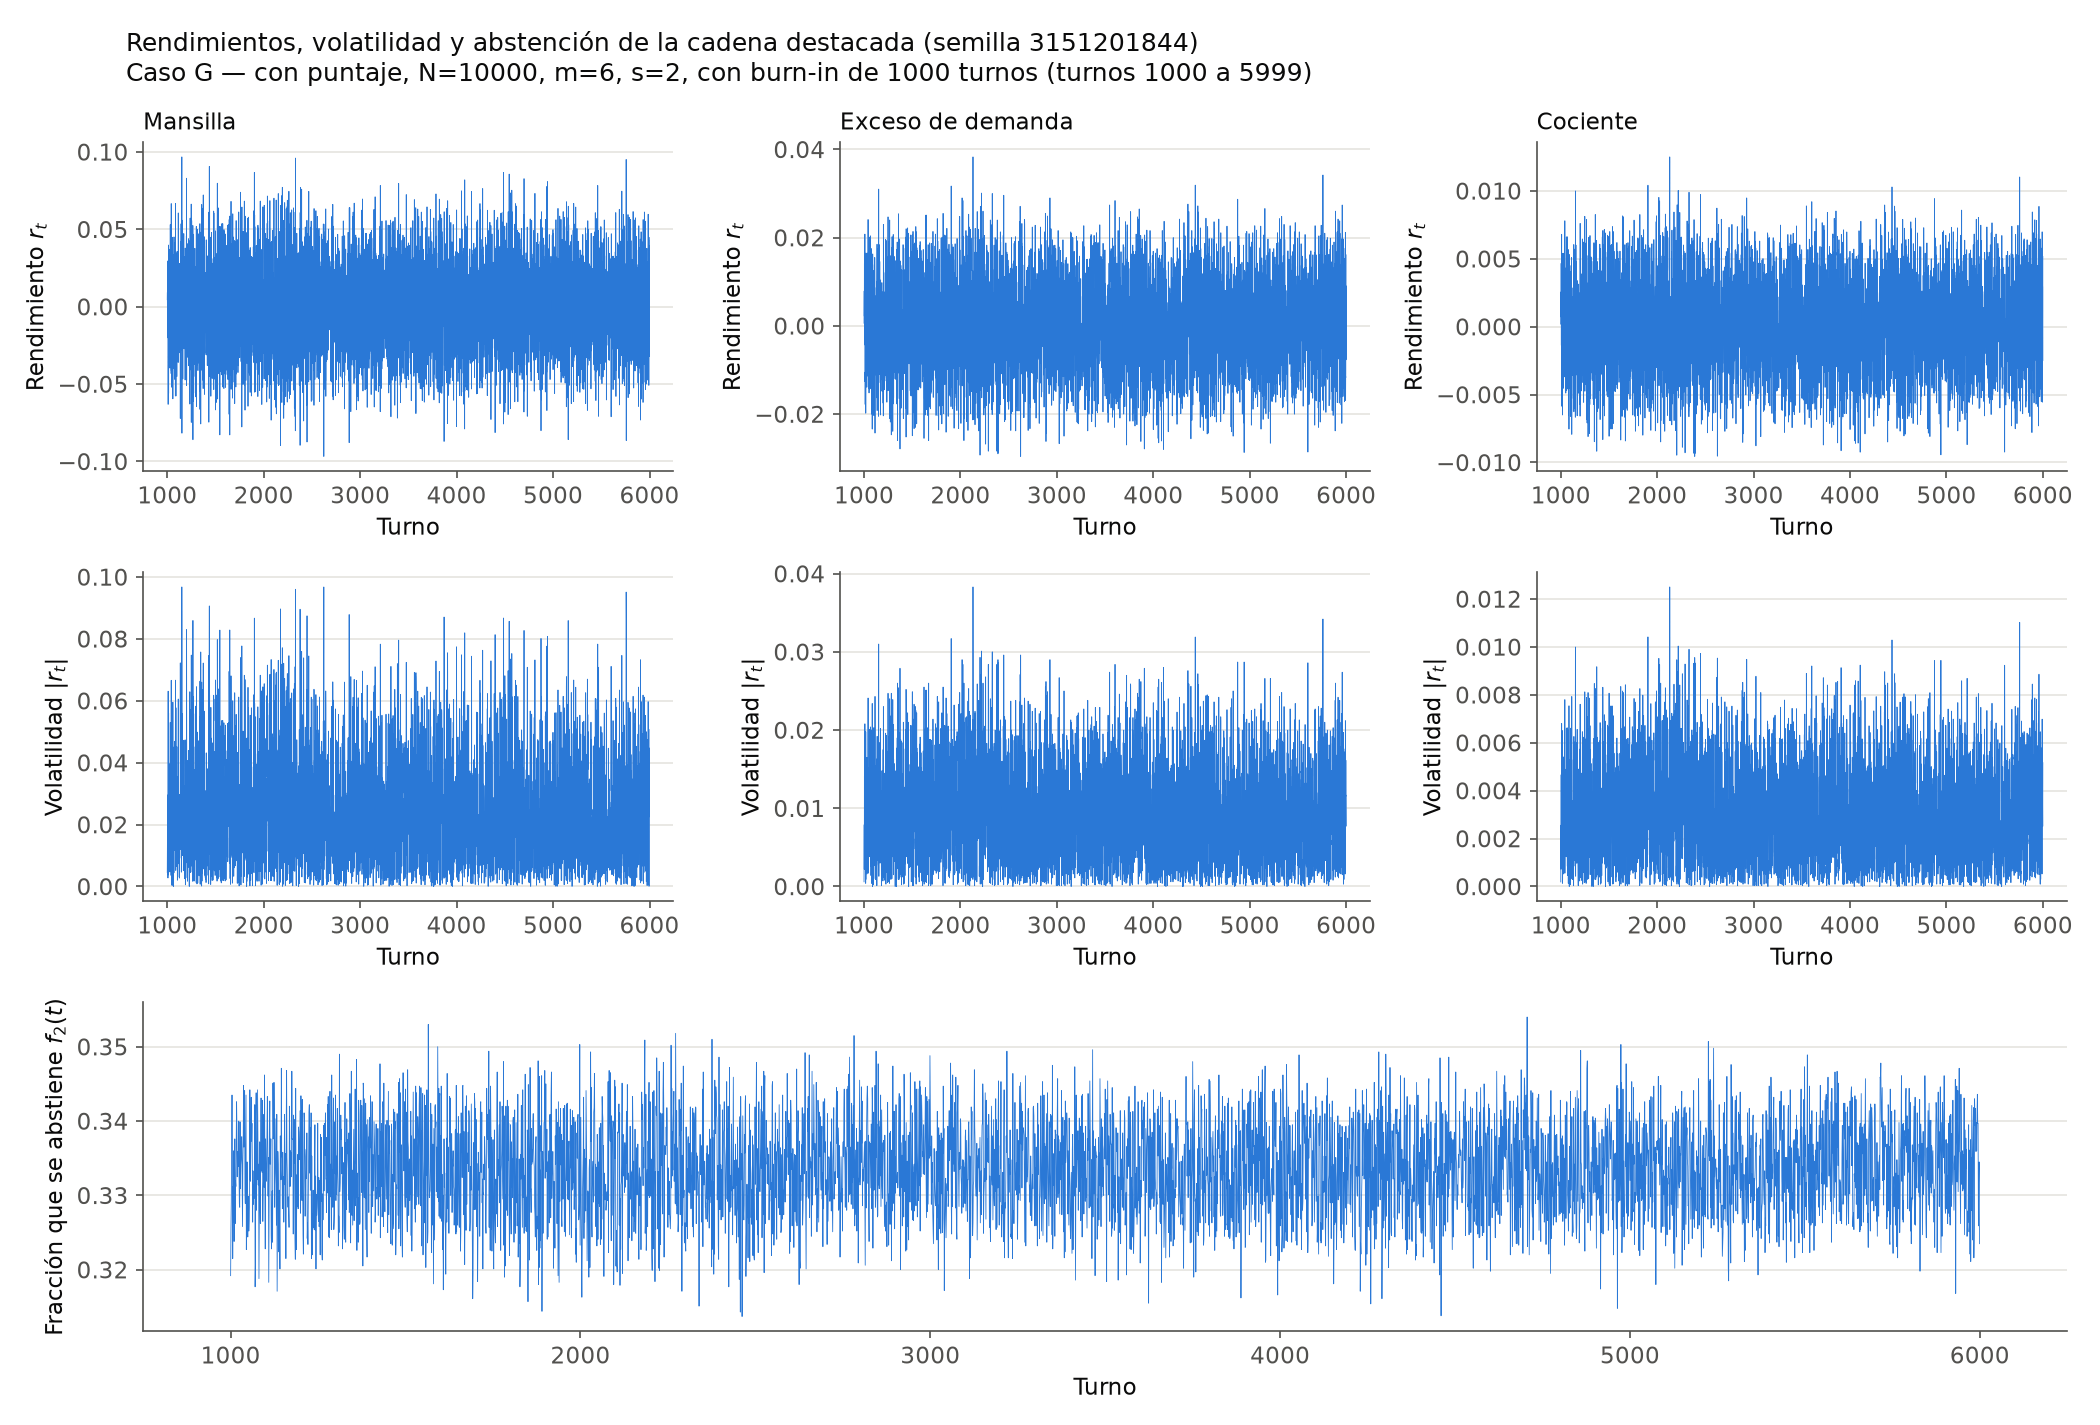
\includegraphics[width=0.85\textwidth]{figuras/Fase9_series_casoG_N10000_m6_s2_con_puntaje_T6000_regla_nueva_con_burnin1000.png}
\caption{Caso G: rendimientos, volatilidad y fracción que se abstiene de la cadena destacada, con burn-in.}
\end{figure}

\begin{figure}[H]
\centering
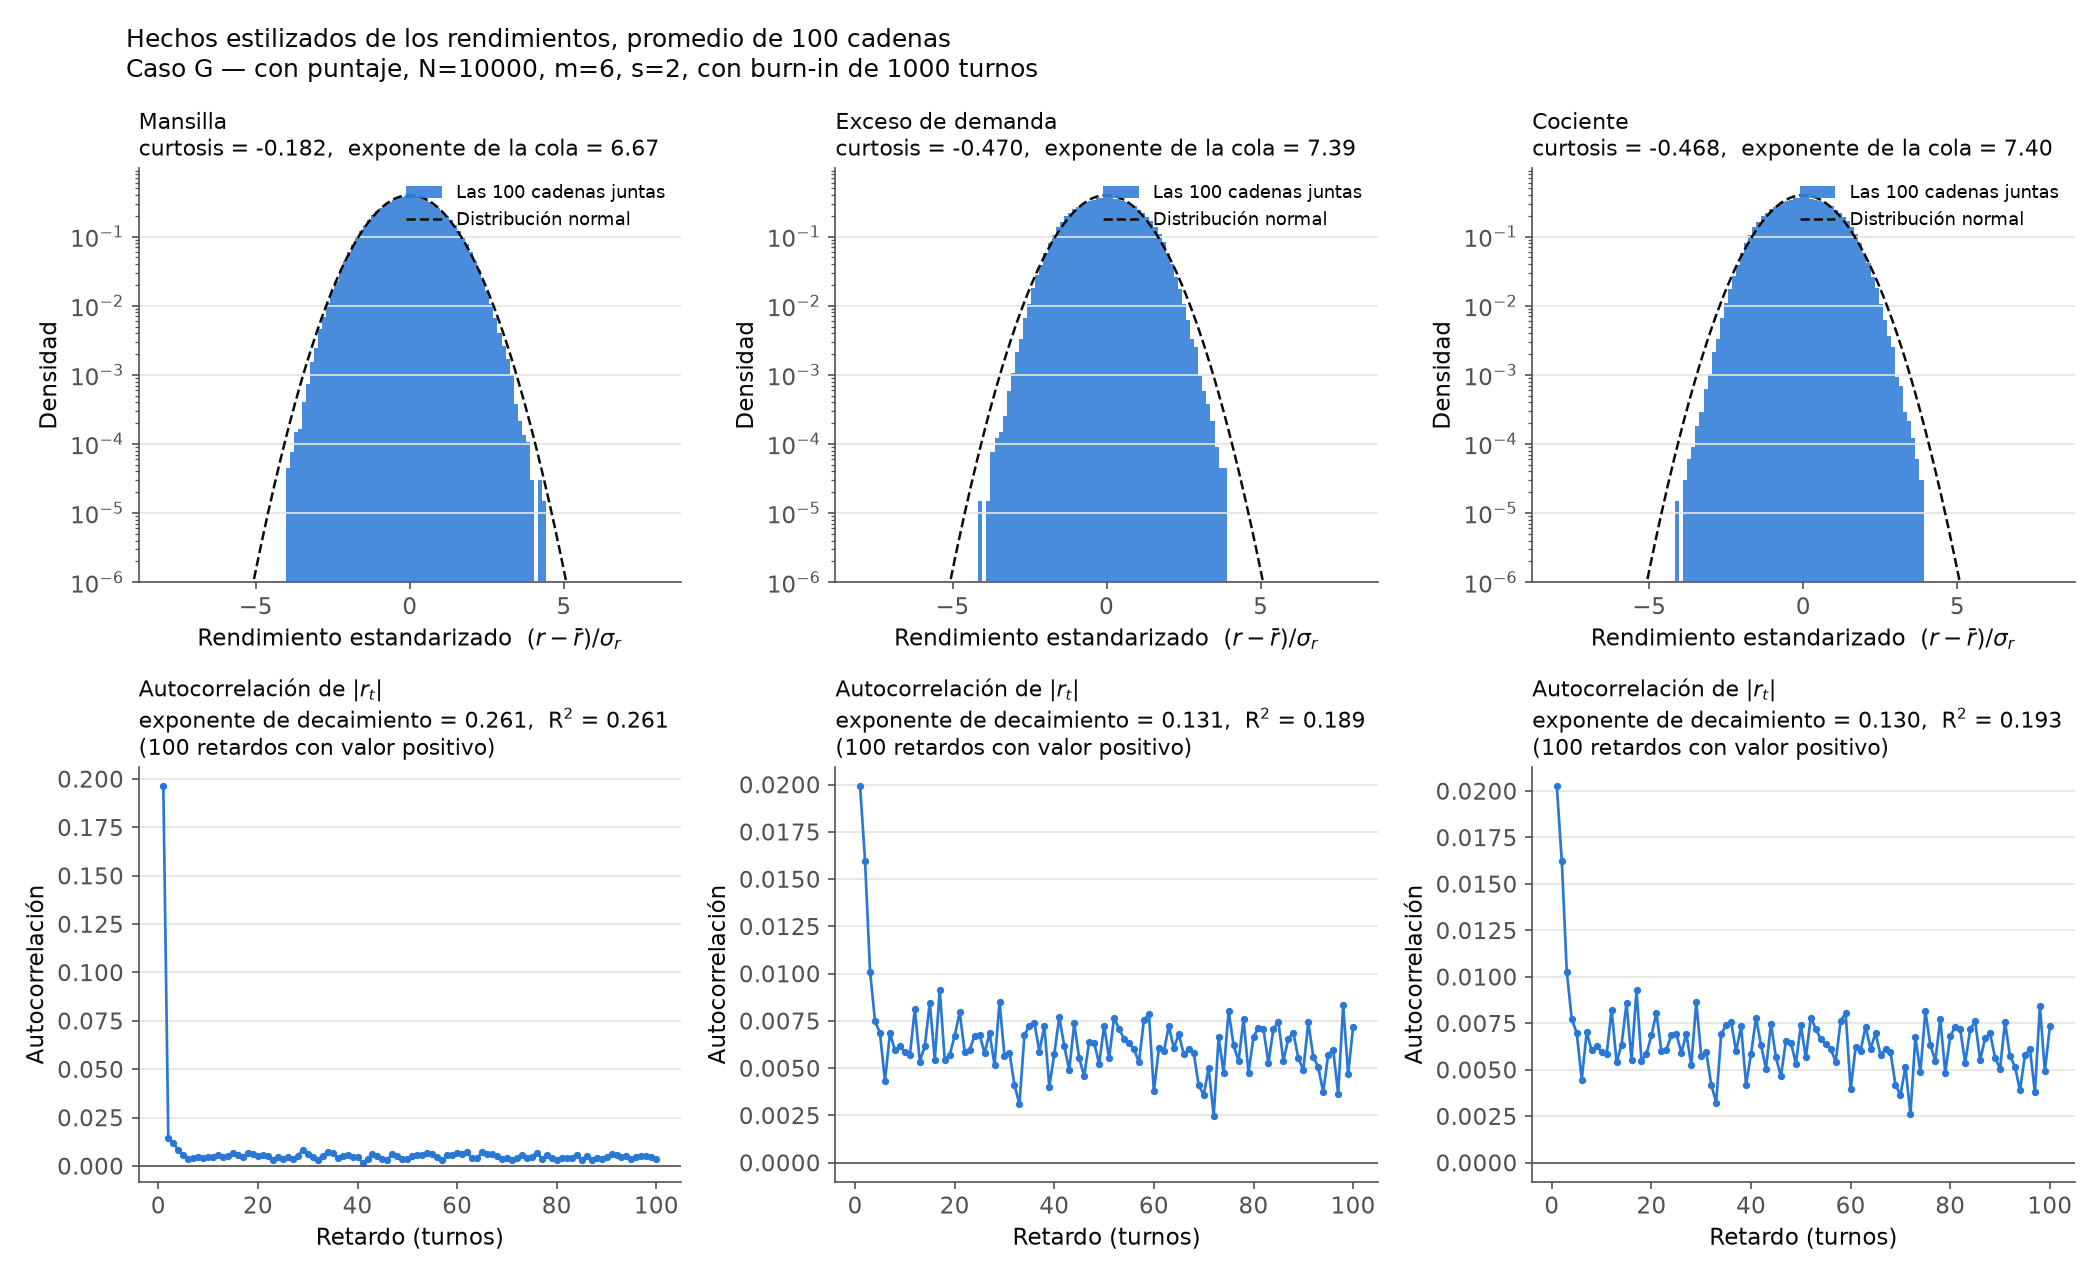
\includegraphics[width=0.85\textwidth]{figuras/Fase9_hechos_estilizados_casoG_N10000_m6_s2_con_puntaje_T6000_regla_nueva_con_burnin1000.png}
\caption{Caso G: hechos estilizados (distribución de los rendimientos y autocorrelación de $|r|$), con burn-in.}
\end{figure}

\begin{figure}[H]
\centering
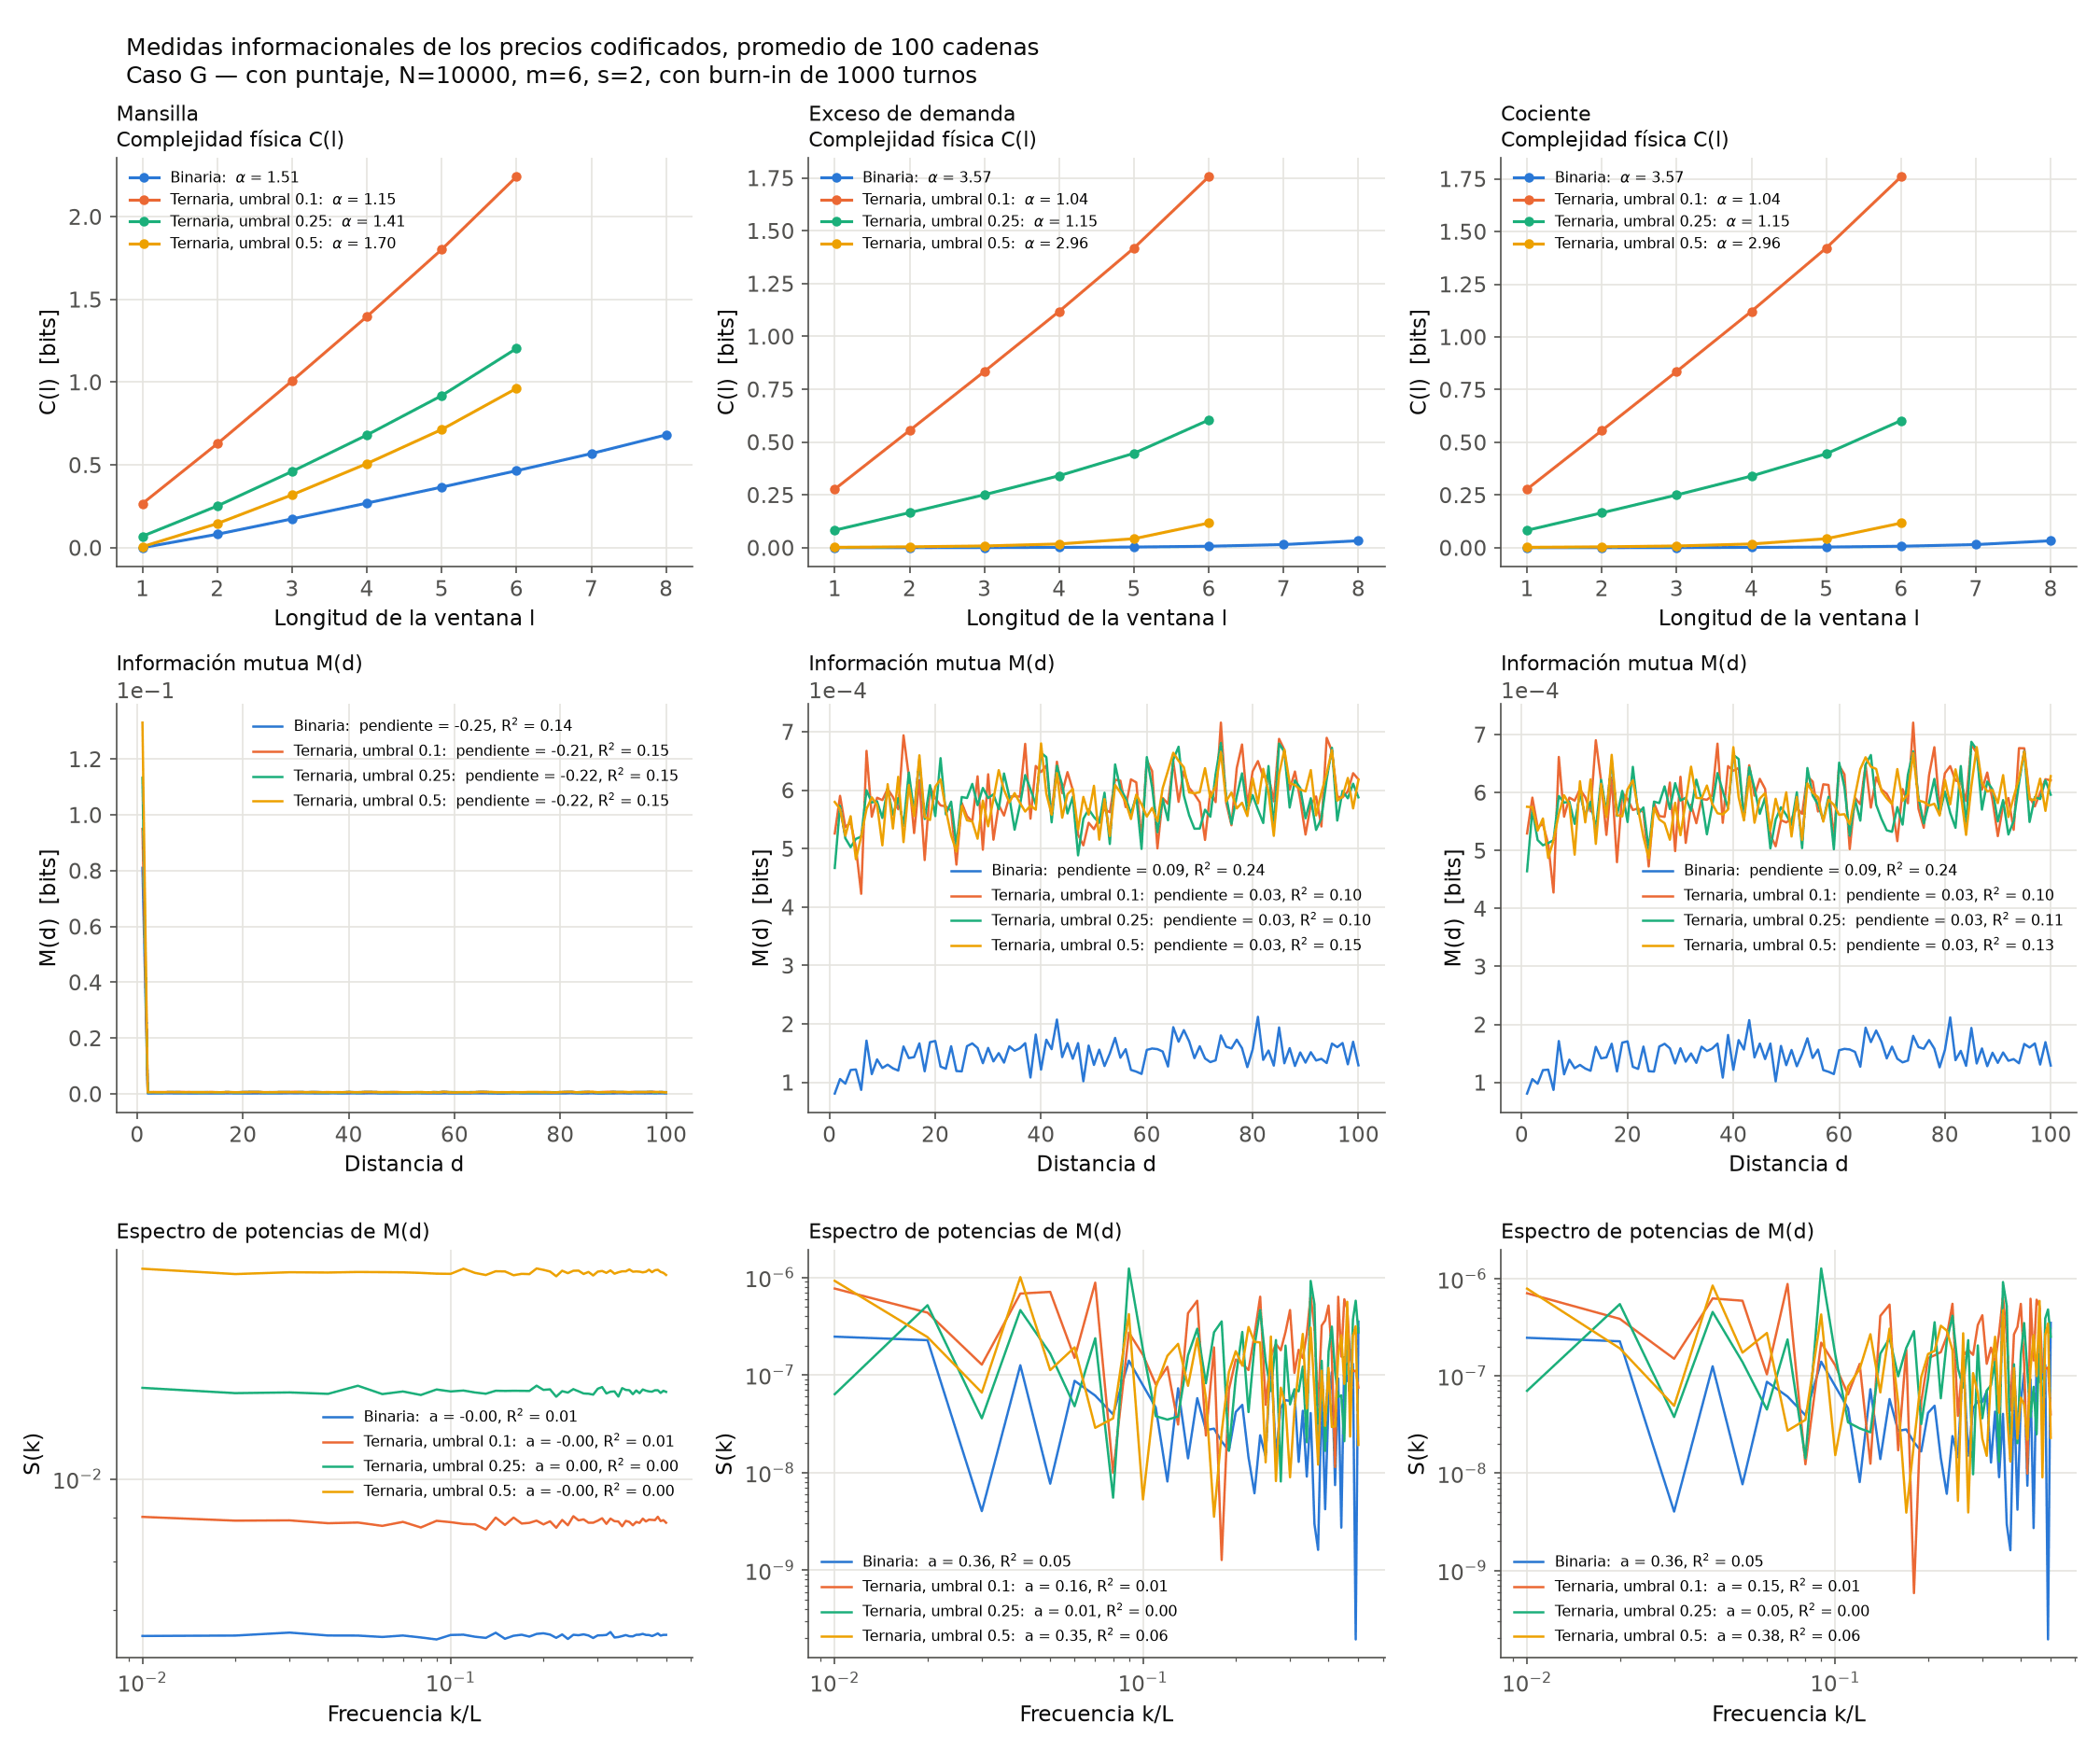
\includegraphics[width=0.85\textwidth]{figuras/Fase9_medidas_informacionales_casoG_N10000_m6_s2_con_puntaje_T6000_regla_nueva_con_burnin1000.png}
\caption{Caso G: medidas informacionales de los precios codificados, con burn-in.}
\end{figure}

\clearpage

\section{Fase 9, $N=10000$: resultados sin burn-in}\label{ap:sinburnin}
\begin{table}[H]
\centering
\footnotesize
\setlength{\tabcolsep}{3.5pt}
\caption{Fase 9, $N=10000$, sin burn-in: hechos estilizados de los rendimientos (mismas columnas que la tabla~\ref{tab:f9hechos}).}\label{tab:f9hechossin}
\begin{adjustbox}{max width=\textwidth}
\begin{tabular}{rrllrrrrrrrrr}
\toprule
Caso & $m$ & Punt. & Precio & $\sigma_r$ & Curtosis & Exp. cola & acf(1) & acf(10) & acf(100) & Exp. acf & $R^2$ acf & Puntos \\
\midrule
A & 2 & sin & Mansilla & $2.08\times10^{-2}$ & $-$0.085 & 6.35 & 0.197 & 0.002 & 0.0023 & 0.903 & 0.443 & 45 \\
A & 2 & sin & Exceso & $7.93\times10^{-3}$ & $-$0.139 & 6.43 & 0.004 & 0.006 & 0.0000 & 0.800 & 0.454 & 70 \\
A & 2 & sin & Cociente & $2.58\times10^{-3}$ & $-$0.138 & 6.43 & 0.004 & 0.006 & 0.0000 & 0.831 & 0.416 & 70 \\
B & 2 & con & Mansilla & 0.297 & 0.461 & 6.47 & 0.245 & $-$0.029 & $-$0.0206 & 0.057 & 0.002 & 29 \\
B & 2 & con & Exceso & 0.106 & $-$0.320 & 8.38 & 0.007 & $-$0.038 & $-$0.0239 & $-$0.369 & 0.121 & 36 \\
B & 2 & con & Cociente & $3.63\times10^{-2}$ & 0.162 & 6.16 & 0.022 & $-$0.041 & $-$0.0253 & $-$0.126 & 0.014 & 36 \\
C & 3 & sin & Mansilla & $2.15\times10^{-2}$ & $-$0.040 & 6.26 & 0.228 & 0.004 & $-$0.0006 & 0.966 & 0.455 & 48 \\
C & 3 & sin & Exceso & $8.06\times10^{-3}$ & $-$0.063 & 6.28 & 0.003 & 0.004 & 0.0001 & 0.756 & 0.482 & 55 \\
C & 3 & sin & Cociente & $2.63\times10^{-3}$ & $-$0.062 & 6.26 & 0.003 & 0.004 & 0.0001 & 0.776 & 0.481 & 55 \\
D & 3 & con & Mansilla & 0.185 & 1.551 & 4.71 & 0.284 & 0.007 & $-$0.0072 & 0.154 & 0.027 & 45 \\
D & 3 & con & Exceso & $6.70\times10^{-2}$ & 0.092 & 5.95 & 0.127 & 0.013 & $-$0.0052 & 0.067 & 0.006 & 49 \\
D & 3 & con & Cociente & $2.25\times10^{-2}$ & 0.745 & 5.15 & 0.147 & 0.015 & $-$0.0062 & 0.105 & 0.013 & 49 \\
E & 4 & con & Mansilla & 0.112 & 2.429 & 3.96 & 0.310 & 0.073 & $-$0.0382 & 1.168 & 0.681 & 45 \\
E & 4 & con & Exceso & $4.06\times10^{-2}$ & 0.687 & 5.15 & 0.203 & 0.091 & $-$0.0497 & 0.951 & 0.669 & 46 \\
E & 4 & con & Cociente & $1.35\times10^{-2}$ & 1.368 & 4.74 & 0.219 & 0.097 & $-$0.0519 & 0.973 & 0.666 & 46 \\
F & 5 & con & Mansilla & $6.67\times10^{-2}$ & 3.862 & 3.51 & 0.332 & 0.138 & 0.0222 & 0.574 & 0.840 & 100 \\
F & 5 & con & Exceso & $2.44\times10^{-2}$ & 1.619 & 4.37 & 0.265 & 0.168 & 0.0302 & 0.524 & 0.816 & 100 \\
F & 5 & con & Cociente & $8.04\times10^{-3}$ & 2.174 & 4.17 & 0.277 & 0.174 & 0.0304 & 0.533 & 0.817 & 100 \\
G & 6 & con & Mansilla & $3.04\times10^{-2}$ & 0.237 & 6.35 & 0.207 & 0.004 & 0.0036 & 0.294 & 0.305 & 100 \\
G & 6 & con & Exceso & $1.13\times10^{-2}$ & 0.321 & 6.75 & 0.018 & 0.005 & 0.0062 & 0.134 & 0.249 & 100 \\
G & 6 & con & Cociente & $3.67\times10^{-3}$ & 0.167 & 6.77 & 0.018 & 0.005 & 0.0065 & 0.133 & 0.257 & 100 \\
\bottomrule
\end{tabular}
\end{adjustbox}
\end{table}


\begin{table}[H]
\centering
\scriptsize
\setlength{\tabcolsep}{3.5pt}
\caption{Fase 9, $N=10000$, sin burn-in: medidas informacionales de la serie binaria (mismas columnas que la tabla~\ref{tab:f9bin}).}\label{tab:f9binsin}
\begin{adjustbox}{max width=\textwidth}
\begin{tabular}{rrllrrrrrrrrrrrr}
\toprule
Caso & $m$ & Punt. & Serie & Frac. 1 & $C(2)$ & $C(8)$ & $\alpha$ & $R^2_C$ & $M(1)$ & $M_{\max}$ & $d_{\max}$ & Pend. $M$ & $R^2_M$ & $a$ & $R^2_S$ \\
\midrule
A & 2 & sin & Mansilla & 0.501 & $9.05\times10^{-2}$ & 0.846 & 1.586 & 0.9921 & $8.79\times10^{-2}$ & $8.79\times10^{-2}$ & 1 & $-$0.830 & 0.613 & 0.321 & 0.932 \\
A & 2 & sin & Acumulados & 0.514 & 0.134 & 1.021 & 1.452 & 0.9973 & $3.49\times10^{-2}$ & $3.49\times10^{-2}$ & 1 & $-$1.125 & 0.897 & 1.344 & 0.815 \\
B & 2 & con & Mansilla & 0.502 & $7.72\times10^{-2}$ & 0.792 & 1.657 & 0.9984 & $7.54\times10^{-2}$ & $7.54\times10^{-2}$ & 1 & $-$0.570 & 0.365 & 0.111 & 0.208 \\
B & 2 & con & Acumulados & 0.501 & $4.24\times10^{-3}$ & 0.357 & 3.346 & 0.9887 & $1.85\times10^{-3}$ & $1.10\times10^{-2}$ & 3 & $-$0.400 & 0.275 & 0.191 & 0.024 \\
C & 3 & sin & Mansilla & 0.498 & $8.89\times10^{-2}$ & 0.789 & 1.552 & 0.9942 & $8.80\times10^{-2}$ & $8.80\times10^{-2}$ & 1 & $-$0.799 & 0.615 & 0.183 & 0.854 \\
C & 3 & sin & Acumulados & 0.495 & $5.49\times10^{-2}$ & 0.552 & 1.680 & 0.9995 & $1.45\times10^{-2}$ & $1.45\times10^{-2}$ & 1 & $-$1.056 & 0.891 & 1.294 & 0.858 \\
D & 3 & con & Mansilla & 0.499 & $7.81\times10^{-2}$ & 0.676 & 1.530 & 0.9941 & $7.78\times10^{-2}$ & $7.78\times10^{-2}$ & 1 & $-$0.509 & 0.408 & 0.020 & 0.276 \\
D & 3 & con & Acumulados & 0.500 & $8.08\times10^{-4}$ & $7.34\times10^{-2}$ & 3.400 & 0.9780 & $3.17\times10^{-4}$ & $2.29\times10^{-3}$ & 4 & $-$0.274 & 0.463 & 0.319 & 0.511 \\
E & 4 & con & Mansilla & 0.500 & $8.13\times10^{-2}$ & 0.677 & 1.502 & 0.9936 & $8.11\times10^{-2}$ & $8.11\times10^{-2}$ & 1 & $-$0.325 & 0.212 & 0.002 & 0.090 \\
E & 4 & con & Acumulados & 0.500 & $2.81\times10^{-4}$ & $3.70\times10^{-2}$ & 3.528 & 0.9707 & $1.25\times10^{-4}$ & $2.57\times10^{-4}$ & 5 & $-$0.004 & 0.001 & 0.319 & 0.070 \\
F & 5 & con & Mansilla & 0.500 & $8.15\times10^{-2}$ & 0.681 & 1.505 & 0.9935 & $8.14\times10^{-2}$ & $8.14\times10^{-2}$ & 1 & $-$0.276 & 0.158 & 0.000 & 0.000 \\
F & 5 & con & Acumulados & 0.499 & $2.19\times10^{-4}$ & $2.99\times10^{-2}$ & 3.502 & 0.9644 & $9.09\times10^{-5}$ & $2.36\times10^{-4}$ & 6 & 0.074 & 0.128 & 0.327 & 0.082 \\
G & 6 & con & Mansilla & 0.500 & $8.11\times10^{-2}$ & 0.676 & 1.503 & 0.9934 & $8.10\times10^{-2}$ & $8.10\times10^{-2}$ & 1 & $-$0.248 & 0.128 & $-$0.001 & 0.055 \\
G & 6 & con & Acumulados & 0.499 & $1.60\times10^{-4}$ & $2.66\times10^{-2}$ & 3.658 & 0.9761 & $7.22\times10^{-5}$ & $1.62\times10^{-4}$ & 81 & 0.104 & 0.321 & 0.320 & 0.062 \\
\bottomrule
\end{tabular}
\end{adjustbox}
\end{table}


\section{Fase 9, $N=10000$: codificación ternaria}\label{ap:ternaria}
\begin{landscape}
Codificación ternaria: 2 si $|r_t|<u\,\sigma_r$; si no, 1 si sube y 0 si baja. $C(l)$ con $l=1,\dots,6$ y ajuste con $l\ge 2$. Solo se muestra la versión con burn-in; la versión sin burn-in está en el CSV de parámetros del apartado 6.7 (filas con \texttt{burn\_in} = 0).

\begin{scriptsize}
\setlength{\tabcolsep}{3pt}
\begin{longtable}{llrrrrrrrrrrrrrrr}
\caption{Fase 9, $N=10000$, con burn-in: medidas informacionales de la serie ternaria para los tres umbrales $u$.}\label{tab:f9ter}\\
\toprule
Caso ($m$, puntaje) & Precio & $u$ & Frac. 0 & Frac. 1 & Frac. 2 & $C(2)$ & $C(6)$ & $\alpha$ & $R^2_C$ & $M(1)$ & $M_{\max}$ & $d_{\max}$ & Pend. $M$ & $R^2_M$ & $a$ & $R^2_S$ \\
\midrule
\endfirsthead
\toprule
Caso ($m$, puntaje) & Precio & $u$ & Frac. 0 & Frac. 1 & Frac. 2 & $C(2)$ & $C(6)$ & $\alpha$ & $R^2_C$ & $M(1)$ & $M_{\max}$ & $d_{\max}$ & Pend. $M$ & $R^2_M$ & $a$ & $R^2_S$ \\
\midrule
\endhead
\bottomrule
\endfoot
A (2, sin) & Mansilla & 0.10 & 0.459 & 0.462 & 0.079 & 0.640 & 2.377 & 1.191 & 0.9999 & 0.104 & 0.104 & 1 & $-$0.548 & 0.501 & 0.335 & 0.931 \\
A (2, sin) & Mansilla & 0.25 & 0.402 & 0.404 & 0.194 & 0.267 & 1.375 & 1.483 & 0.9992 & 0.124 & 0.124 & 1 & $-$0.595 & 0.529 & 0.348 & 0.932 \\
A (2, sin) & Mansilla & 0.50 & 0.311 & 0.312 & 0.377 & 0.163 & 1.152 & 1.769 & 0.9957 & 0.145 & 0.145 & 1 & $-$0.640 & 0.549 & 0.371 & 0.931 \\
A (2, sin) & Exceso & 0.10 & 0.450 & 0.478 & 0.072 & 0.713 & 2.540 & 1.153 & 1.0000 & $3.83\times10^{-2}$ & $3.83\times10^{-2}$ & 1 & $-$0.737 & 0.803 & 1.358 & 0.817 \\
A (2, sin) & Exceso & 0.25 & 0.396 & 0.424 & 0.180 & 0.328 & 1.419 & 1.324 & 0.9998 & $4.22\times10^{-2}$ & $4.22\times10^{-2}$ & 1 & $-$0.792 & 0.856 & 1.340 & 0.827 \\
A (2, sin) & Exceso & 0.50 & 0.312 & 0.337 & 0.351 & 0.172 & 0.932 & 1.522 & 0.9997 & $4.31\times10^{-2}$ & $4.31\times10^{-2}$ & 1 & $-$0.823 & 0.888 & 1.331 & 0.839 \\
A (2, sin) & Cociente & 0.10 & 0.450 & 0.478 & 0.072 & 0.712 & 2.538 & 1.153 & 1.0000 & $3.84\times10^{-2}$ & $3.84\times10^{-2}$ & 1 & $-$0.737 & 0.803 & 1.357 & 0.817 \\
A (2, sin) & Cociente & 0.25 & 0.396 & 0.424 & 0.180 & 0.328 & 1.421 & 1.325 & 0.9998 & $4.22\times10^{-2}$ & $4.22\times10^{-2}$ & 1 & $-$0.794 & 0.857 & 1.342 & 0.827 \\
A (2, sin) & Cociente & 0.50 & 0.312 & 0.337 & 0.351 & 0.173 & 0.934 & 1.524 & 0.9997 & $4.32\times10^{-2}$ & $4.32\times10^{-2}$ & 1 & $-$0.823 & 0.888 & 1.333 & 0.838 \\
B (2, con) & Mansilla & 0.10 & 0.347 & 0.339 & 0.314 & 0.157 & 1.466 & 2.020 & 0.9997 & 0.141 & 0.141 & 1 & $-$0.453 & 0.369 & 0.204 & 0.320 \\
B (2, con) & Mansilla & 0.25 & 0.301 & 0.291 & 0.408 & 0.206 & 1.781 & 1.955 & 0.9999 & 0.160 & 0.160 & 1 & $-$0.475 & 0.374 & 0.233 & 0.379 \\
B (2, con) & Mansilla & 0.50 & 0.292 & 0.289 & 0.419 & 0.222 & 1.836 & 1.918 & 0.9999 & 0.164 & 0.164 & 1 & $-$0.486 & 0.390 & 0.234 & 0.415 \\
B (2, con) & Exceso & 0.10 & 0.284 & 0.275 & 0.441 & 0.121 & 0.999 & 1.909 & 0.9886 & $1.78\times10^{-2}$ & $2.13\times10^{-2}$ & 27 & $-$0.279 & 0.272 & 0.402 & 0.129 \\
B (2, con) & Exceso & 0.25 & 0.230 & 0.217 & 0.554 & 0.362 & 1.850 & 1.476 & 0.9936 & $2.74\times10^{-2}$ & $2.74\times10^{-2}$ & 1 & $-$0.292 & 0.255 & 0.474 & 0.225 \\
B (2, con) & Exceso & 0.50 & 0.229 & 0.216 & 0.555 & 0.366 & 1.865 & 1.474 & 0.9937 & $2.75\times10^{-2}$ & $2.75\times10^{-2}$ & 1 & $-$0.292 & 0.254 & 0.467 & 0.218 \\
B (2, con) & Cociente & 0.10 & 0.278 & 0.269 & 0.453 & 0.140 & 1.065 & 1.835 & 0.9889 & $1.85\times10^{-2}$ & $2.21\times10^{-2}$ & 27 & $-$0.278 & 0.273 & 0.400 & 0.132 \\
B (2, con) & Cociente & 0.25 & 0.229 & 0.217 & 0.554 & 0.363 & 1.854 & 1.475 & 0.9937 & $2.74\times10^{-2}$ & $2.74\times10^{-2}$ & 1 & $-$0.292 & 0.255 & 0.474 & 0.225 \\
B (2, con) & Cociente & 0.50 & 0.229 & 0.216 & 0.555 & 0.366 & 1.865 & 1.474 & 0.9937 & $2.75\times10^{-2}$ & $2.75\times10^{-2}$ & 1 & $-$0.292 & 0.254 & 0.467 & 0.218 \\
C (3, sin) & Mansilla & 0.10 & 0.462 & 0.458 & 0.079 & 0.633 & 2.316 & 1.177 & 1.0000 & 0.103 & 0.103 & 1 & $-$0.533 & 0.523 & 0.190 & 0.847 \\
C (3, sin) & Mansilla & 0.25 & 0.403 & 0.400 & 0.196 & 0.259 & 1.300 & 1.460 & 0.9996 & 0.123 & 0.123 & 1 & $-$0.582 & 0.553 & 0.202 & 0.869 \\
C (3, sin) & Mansilla & 0.50 & 0.310 & 0.308 & 0.382 & 0.161 & 1.094 & 1.732 & 0.9975 & 0.143 & 0.143 & 1 & $-$0.638 & 0.583 & 0.224 & 0.879 \\
C (3, sin) & Exceso & 0.10 & 0.467 & 0.456 & 0.077 & 0.600 & 2.087 & 1.131 & 0.9993 & $1.64\times10^{-2}$ & $1.64\times10^{-2}$ & 1 & $-$0.625 & 0.779 & 1.275 & 0.831 \\
C (3, sin) & Exceso & 0.25 & 0.410 & 0.399 & 0.191 & 0.211 & 0.947 & 1.355 & 0.9969 & $1.77\times10^{-2}$ & $1.77\times10^{-2}$ & 1 & $-$0.660 & 0.798 & 1.302 & 0.841 \\
C (3, sin) & Exceso & 0.50 & 0.320 & 0.309 & 0.372 & $8.43\times10^{-2}$ & 0.554 & 1.701 & 0.9962 & $1.81\times10^{-2}$ & $1.81\times10^{-2}$ & 1 & $-$0.671 & 0.794 & 1.347 & 0.837 \\
C (3, sin) & Cociente & 0.10 & 0.467 & 0.456 & 0.077 & 0.600 & 2.086 & 1.132 & 0.9993 & $1.63\times10^{-2}$ & $1.63\times10^{-2}$ & 1 & $-$0.625 & 0.779 & 1.278 & 0.831 \\
C (3, sin) & Cociente & 0.25 & 0.410 & 0.399 & 0.191 & 0.211 & 0.946 & 1.356 & 0.9969 & $1.77\times10^{-2}$ & $1.77\times10^{-2}$ & 1 & $-$0.661 & 0.799 & 1.304 & 0.841 \\
C (3, sin) & Cociente & 0.50 & 0.319 & 0.309 & 0.372 & $8.45\times10^{-2}$ & 0.556 & 1.702 & 0.9963 & $1.81\times10^{-2}$ & $1.81\times10^{-2}$ & 1 & $-$0.671 & 0.793 & 1.350 & 0.836 \\
D (3, con) & Mansilla & 0.10 & 0.366 & 0.364 & 0.270 & 0.152 & 0.989 & 1.686 & 0.9987 & 0.122 & 0.122 & 1 & $-$0.346 & 0.299 & 0.037 & 0.572 \\
D (3, con) & Mansilla & 0.25 & 0.289 & 0.286 & 0.426 & 0.212 & 1.378 & 1.695 & 0.9982 & 0.156 & 0.156 & 1 & $-$0.305 & 0.183 & 0.054 & 0.710 \\
D (3, con) & Mansilla & 0.50 & 0.278 & 0.277 & 0.444 & 0.243 & 1.521 & 1.664 & 0.9984 & 0.163 & 0.163 & 1 & $-$0.294 & 0.162 & 0.057 & 0.724 \\
D (3, con) & Exceso & 0.10 & 0.334 & 0.336 & 0.330 & $1.03\times10^{-2}$ & 0.209 & 2.695 & 0.9796 & $3.75\times10^{-3}$ & $3.75\times10^{-3}$ & 1 & $-$0.169 & 0.207 & 1.339 & 0.628 \\
D (3, con) & Exceso & 0.25 & 0.228 & 0.239 & 0.534 & 0.264 & 1.049 & 1.241 & 0.9950 & $9.90\times10^{-3}$ & $9.90\times10^{-3}$ & 1 & $-$0.115 & 0.035 & 1.173 & 0.818 \\
D (3, con) & Exceso & 0.50 & 0.216 & 0.229 & 0.555 & 0.321 & 1.240 & 1.218 & 0.9961 & $1.16\times10^{-2}$ & $1.16\times10^{-2}$ & 1 & $-$0.105 & 0.025 & 1.164 & 0.843 \\
D (3, con) & Cociente & 0.10 & 0.329 & 0.332 & 0.339 & $1.09\times10^{-2}$ & 0.214 & 2.670 & 0.9800 & $3.72\times10^{-3}$ & $3.72\times10^{-3}$ & 1 & $-$0.172 & 0.209 & 1.369 & 0.631 \\
D (3, con) & Cociente & 0.25 & 0.226 & 0.237 & 0.537 & 0.272 & 1.078 & 1.237 & 0.9952 & $9.96\times10^{-3}$ & $9.96\times10^{-3}$ & 1 & $-$0.112 & 0.033 & 1.183 & 0.821 \\
D (3, con) & Cociente & 0.50 & 0.216 & 0.229 & 0.555 & 0.321 & 1.240 & 1.218 & 0.9961 & $1.16\times10^{-2}$ & $1.16\times10^{-2}$ & 1 & $-$0.105 & 0.025 & 1.164 & 0.843 \\
E (4, con) & Mansilla & 0.10 & 0.407 & 0.407 & 0.187 & 0.268 & 1.250 & 1.391 & 0.9997 & 0.112 & 0.112 & 1 & $-$0.297 & 0.272 & 0.009 & 0.488 \\
E (4, con) & Mansilla & 0.25 & 0.315 & 0.314 & 0.371 & 0.153 & 1.055 & 1.744 & 0.9972 & 0.142 & 0.142 & 1 & $-$0.478 & 0.509 & 0.047 & 0.714 \\
E (4, con) & Mansilla & 0.50 & 0.269 & 0.267 & 0.464 & 0.270 & 1.548 & 1.585 & 0.9985 & 0.163 & 0.163 & 1 & $-$0.562 & 0.558 & 0.076 & 0.754 \\
E (4, con) & Exceso & 0.10 & 0.392 & 0.392 & 0.216 & $9.94\times10^{-2}$ & 0.423 & 1.282 & 0.9834 & $1.40\times10^{-3}$ & $1.40\times10^{-3}$ & 1 & $-$0.135 & 0.539 & 1.453 & 0.630 \\
E (4, con) & Exceso & 0.25 & 0.278 & 0.280 & 0.442 & $8.13\times10^{-2}$ & 0.409 & 1.434 & 0.9842 & $5.65\times10^{-3}$ & $5.65\times10^{-3}$ & 1 & $-$0.386 & 0.514 & 1.378 & 0.912 \\
E (4, con) & Exceso & 0.50 & 0.224 & 0.226 & 0.550 & 0.301 & 1.138 & 1.198 & 0.9966 & $1.31\times10^{-2}$ & $1.31\times10^{-2}$ & 1 & $-$0.513 & 0.435 & 1.366 & 0.953 \\
E (4, con) & Cociente & 0.10 & 0.390 & 0.390 & 0.220 & $9.30\times10^{-2}$ & 0.405 & 1.301 & 0.9819 & $1.39\times10^{-3}$ & $1.39\times10^{-3}$ & 1 & $-$0.135 & 0.538 & 1.474 & 0.606 \\
E (4, con) & Cociente & 0.25 & 0.276 & 0.278 & 0.447 & $8.79\times10^{-2}$ & 0.431 & 1.413 & 0.9850 & $5.61\times10^{-3}$ & $5.61\times10^{-3}$ & 1 & $-$0.388 & 0.519 & 1.389 & 0.910 \\
E (4, con) & Cociente & 0.50 & 0.223 & 0.226 & 0.551 & 0.303 & 1.146 & 1.197 & 0.9967 & $1.31\times10^{-2}$ & $1.31\times10^{-2}$ & 1 & $-$0.513 & 0.435 & 1.369 & 0.953 \\
F (5, con) & Mansilla & 0.10 & 0.439 & 0.439 & 0.121 & 0.448 & 1.741 & 1.229 & 0.9999 & 0.101 & 0.101 & 1 & $-$0.239 & 0.189 & 0.000 & 0.004 \\
F (5, con) & Mansilla & 0.25 & 0.359 & 0.359 & 0.282 & 0.143 & 0.931 & 1.691 & 0.9979 & 0.124 & 0.124 & 1 & $-$0.374 & 0.423 & 0.009 & 0.586 \\
F (5, con) & Mansilla & 0.50 & 0.263 & 0.263 & 0.474 & 0.264 & 1.369 & 1.492 & 0.9991 & 0.141 & 0.141 & 1 & $-$0.569 & 0.736 & 0.032 & 0.821 \\
F (5, con) & Exceso & 0.10 & 0.433 & 0.432 & 0.134 & 0.301 & 1.015 & 1.091 & 0.9968 & $7.62\times10^{-4}$ & $8.27\times10^{-4}$ & 10 & $-$0.048 & 0.312 & 0.480 & 0.084 \\
F (5, con) & Exceso & 0.25 & 0.345 & 0.344 & 0.310 & $6.91\times10^{-3}$ & 0.146 & 2.697 & 0.9662 & $2.47\times10^{-3}$ & $2.47\times10^{-3}$ & 1 & $-$0.259 & 0.887 & 1.493 & 0.742 \\
F (5, con) & Exceso & 0.50 & 0.254 & 0.253 & 0.493 & 0.166 & 0.678 & 1.259 & 0.9932 & $8.47\times10^{-3}$ & $8.47\times10^{-3}$ & 1 & $-$0.431 & 0.841 & 1.529 & 0.951 \\
F (5, con) & Cociente & 0.10 & 0.432 & 0.431 & 0.136 & 0.295 & 0.995 & 1.093 & 0.9967 & $7.32\times10^{-4}$ & $8.25\times10^{-4}$ & 10 & $-$0.044 & 0.295 & 0.448 & 0.074 \\
F (5, con) & Cociente & 0.25 & 0.343 & 0.343 & 0.314 & $5.85\times10^{-3}$ & 0.143 & 2.831 & 0.9689 & $2.43\times10^{-3}$ & $2.43\times10^{-3}$ & 1 & $-$0.254 & 0.879 & 1.435 & 0.757 \\
F (5, con) & Cociente & 0.50 & 0.252 & 0.251 & 0.497 & 0.173 & 0.700 & 1.251 & 0.9934 & $8.42\times10^{-3}$ & $8.42\times10^{-3}$ & 1 & $-$0.430 & 0.839 & 1.545 & 0.947 \\
G (6, con) & Mansilla & 0.10 & 0.461 & 0.460 & 0.079 & 0.628 & 2.241 & 1.154 & 0.9999 & $9.50\times10^{-2}$ & $9.50\times10^{-2}$ & 1 & $-$0.213 & 0.151 & $-$0.001 & 0.005 \\
G (6, con) & Mansilla & 0.25 & 0.403 & 0.403 & 0.194 & 0.252 & 1.204 & 1.413 & 0.9996 & 0.113 & 0.113 & 1 & $-$0.220 & 0.150 & 0.000 & 0.001 \\
G (6, con) & Mansilla & 0.50 & 0.312 & 0.311 & 0.377 & 0.146 & 0.962 & 1.705 & 0.9973 & 0.133 & 0.133 & 1 & $-$0.223 & 0.147 & 0.000 & 0.002 \\
G (6, con) & Exceso & 0.10 & 0.463 & 0.462 & 0.075 & 0.555 & 1.756 & 1.043 & 0.9993 & $5.26\times10^{-4}$ & $7.16\times10^{-4}$ & 74 & 0.031 & 0.100 & 0.165 & 0.014 \\
G (6, con) & Exceso & 0.25 & 0.409 & 0.409 & 0.182 & 0.166 & 0.604 & 1.153 & 0.9918 & $4.67\times10^{-4}$ & $6.81\times10^{-4}$ & 74 & 0.026 & 0.095 & 0.015 & 0.000 \\
G (6, con) & Exceso & 0.50 & 0.322 & 0.322 & 0.355 & $4.13\times10^{-3}$ & 0.117 & 2.958 & 0.9452 & $5.80\times10^{-4}$ & $6.80\times10^{-4}$ & 40 & 0.030 & 0.154 & 0.346 & 0.056 \\
G (6, con) & Cociente & 0.10 & 0.463 & 0.462 & 0.074 & 0.556 & 1.760 & 1.043 & 0.9993 & $5.29\times10^{-4}$ & $7.20\times10^{-4}$ & 74 & 0.030 & 0.095 & 0.147 & 0.009 \\
G (6, con) & Cociente & 0.25 & 0.409 & 0.409 & 0.182 & 0.165 & 0.603 & 1.153 & 0.9918 & $4.64\times10^{-4}$ & $6.87\times10^{-4}$ & 85 & 0.027 & 0.106 & 0.050 & 0.001 \\
G (6, con) & Cociente & 0.50 & 0.322 & 0.322 & 0.355 & $4.11\times10^{-3}$ & 0.117 & 2.965 & 0.9457 & $5.75\times10^{-4}$ & $6.78\times10^{-4}$ & 86 & 0.028 & 0.133 & 0.376 & 0.060 \\
\end{longtable}
\end{scriptsize}
\end{landscape}


\end{document}
